\documentclass[a4,12pt,openright]{book}
\usepackage[english,portuguese,brazilian,brazil]{babel}
\usepackage[latin1]{inputenc}
\usepackage[T1]{fontenc}
%\usepackage{pxfonts}
%\usepackage{lmodern}
%\usepackage{textcomp}
\usepackage{fancyhdr}
\usepackage{psboxit}
\usepackage{hyphenat}
  \usepackage[stepnumber=1,style=\script,frameround=fttt]{listings}
\usepackage{keystroke}
\usepackage{xy}
%\input xy
\xyoption{all}
\addtolength{\headheight}{3pt}
%% \addtolength{\textwidth}{\marginparwidth}
%% \addtolength{\marginparwidth}{-\marginparwidth}
%% \addtolength{\textwidth}{-4cm}
%% \addtolength{\marginparwidth}{4cm}


\makeatletter
\def\cleardoublepage{\clearpage\if@twoside \ifodd\c@page\else
  \hbox{}
  \vfill
  \begin{center}
    \par\mbox{}
  \end{center}
  \vfill
  \thispagestyle{empty}
  \newpage\fi}
\makeatother


    \pagestyle{fancy}                       % Sets fancy header and footer
    \fancyfoot{}                            % Delete current footer settings
    \renewcommand{\chaptermark}[1]{         % Lower Case Chapter marker style
      \markboth{\chaptername\ \thechapter.\ #1}{}} %
    \renewcommand{\sectionmark}[1]{         % Lower case Section marker style
      \markright{\thesection.\ #1}}         %
    \fancyhead[LE,RO]{\bfseries\thepage}    % Page number (boldface) in left on even
                                            % pages and right on odd pages
    \fancyhead[RE]{\bfseries\leftmark}      % Chapter in the right on even pages
    \fancyhead[LO]{\bfseries\rightmark}     % Section in the left on odd pages
    \renewcommand{\headrulewidth}{0.3pt}    % Width of head rule

\usepackage{float}      
\usepackage{fancyvrb}

%===== C�digos Fonte =====
\newenvironment{codeverbatim}{\VerbatimEnvironment \small
   \begin{Verbatim}[xleftmargin=20mm]}
   {\end{Verbatim}}
%=======
\floatstyle{plain}  % tipos: plain, boxed, ruled
\newfloat{codigo}{tbp}{lop}[section]  % numera os captions com  n�mero de se��o.
\floatname{codigo}{Trecho de C�digo}
% nome para ser usado no sum�rio
\newcommand{\listofcodename}{Lista de Trechos de C�digo}
%=========================

\hyphenation{Ci-�n-cias En-t�o pa-re-�am a-dap-ta-��o di-re-t�-rios
a-pro-vei-tar r�-gi-do GNU  Li-nux di-re-t�-rios di-re-t�-rio sa-la-da
pro-ces-sos Li-nux ne-ces-s�-rios fa-lhas pro-prie-t�-rios}

%\ifpdf
%    \usepackage[pdftex]{graphicx}
    %\usepackage[pdftex, bookmarks=true, colorlinks=false, hyperindex=false]{hyperref}
%\else
    \usepackage[dvips]{graphicx}
%    \usepackage[dvips, bookmarks=true, colorlinks=false, hyperindex=false]{hyperref}
%\fi
\usepackage[alf,abnt-etal-text=emph]{abntcite}
\begin{document}
\title{Uma Introdu��o ao GNU/Linux}
\author{F�bio Emilio Costa}
\date{\today}
\frontmatter
\newcommand{\Meta}{\keystroke{Meta}}
\begin{titlepage}
\par\mbox{}
\vspace{5cm}
\begin{flushright}
	\Huge{\textbf{\emph{Uma Introdu��o ao GNU/Linux}}}\par
	\rule[10pt]{\textwidth}{2.5pt}
	\Large{\textit{F�bio Emilio Costa}}\par
	\vfill
\end{flushright}
\end{titlepage}

\begin{titlepage}
\par\mbox{}
\vfill


\framebox[\textwidth]{
\begin{minipage}[t]{\textwidth}
\begin{center}
\begin{Large}
	\textbf{Esse documento  � licenciado segundo  Creative Commons
          \textsc{Atribui��o-Compartilhamento  pela mesma  licen�a 2.5
            Brasil}}\par
\end{Large}
\end{center}

Voc� pode:

\begin{itemize}
\item copiar, distribuir, exibir e executar a obra
\item criar obras derivadas
\item fazer uso comercial da obra
\end{itemize}

Sob as seguintes condi��es:

\begin{itemize} 	
\item \textbf{Atribui��o.} Voc� deve dar cr�dito ao autor original, da
  forma especificada pelo autor ou licenciante. 
\item \textbf{Compartilhamento  pela mesma Licen�a.}  Se voc� alterar,
  transformar, ou criar outra obra com base nesta, voc� somente poder�
  distribuir a obra resultante sob uma licen�a id�ntica a esta.
\end{itemize}
\begin{itemize}
\item Para cada novo uso  ou distribui��o, voc� deve deixar claro para
  outros os termos da licen�a desta obra.
\item Qualquer  uma destas condi��es podem ser  renunciadas, desde que
  Voc� obtenha permiss�o do autor.
\end{itemize} 	

Qualquer direito de uso leg�timo  (ou ``fair use'') concedido por lei,
ou qualquer outro direito protegido  pela legisla��o local, n�o s�o em
hip�tese alguma afetados pelo disposto acima.
\end{minipage}
}
\vfill
\begin{figure}[h]
	\centering
		\includegraphics*{cc}
\end{figure}
\end{titlepage}


\sloppy
\tableofcontents
				\fussy
\listoftables
\listoffigures
\addcontentsline{toc}{chapter}{\listofcodename}
\listof{codigo}{\listofcodename}  % Lista de C�digos 

\chapter{Introdu��o}

GNU/Linux (ou apenas \emph{Linux})  n�o � mais \emph{apenas} o futuro,
mas  sim  tamb�m �  uma  alternativa  s�ria  e vi�vel  para  ambientes
computacionais   que    precisem   de   alta    \emph{performance}   e
confiabilidade   mas   n�o   possuem   condi��es   para   montar   uma
infraestrutura  baseada em  sistemas como  o Windows  e a  maioria das
variantes  do Unix. Baseado  em \emph{software  livre}, ele  � barato,
confi�vel e  poderoso, al�m de oferecer a  oportunidade de aprendizado
com  o seu  c�digo  fonte.  Por�m,  ele  n�o �  exatamente simples  de
aprender,  uma vez que  s�o muitos  comandos, programas  e utilit�rios
(mais    de    3000    em    uma   distribui��o    GNU/Linux    t�pica
atualmente)\footnote{Abril de 2006}.

Essa  � uma  apostila b�sica  do GNU/Linux,  que foi  produzida  com o
objetivo de servir de refer�ncia para  um curso b�sico no mesmo, e tem
como objetivo ser \emph{apenas} uma  introdu��o ao uso do GNU/Linux. O
objetivo  final dessa  apostila �  oferecer  as condi��es  para que  a
pessoa possa seguir a diante  no GNU/Linux sem problemas. Em resumo, o
objetivo  aqui �  oferecer  o ``caminho  das  pedras'', explicando  os
principais recursos do mesmo de maneira r�pida e sucinta.

Essa  apostila foi desenvolvida  para ser  adotada em  um curso  de 20
horas e  sem ser voltada  a nenhuma distribui��o em  especial, podendo
ser  adotada  aquela  que  o  tutor  (ou mesmo  o  aluno)  achar  mais
adequada. A id�ia  � que o aluno saia com  alguns conceitos e comandos
�teis para ``caminhar por suas pr�prias pernas'', al�m de contar com a
sugest�o  de  recursos �teis  e  comandos  alternativos  para o  aluno
pesquisar.

N�o � minha inten��o aqui  mostrar todas as potencialidades e comandos
do GNU/Linux, at� porque n�o  seria poss�vel fazer isso. Como exemplo,
o   projeto   \emph{Linux   Documentation  Project}\cite{LDP2006}   j�
disponibiliza mais de 20  mil p�ginas em documenta��o sobre GNU/Linux,
boa  parte delas traduzida  para outros  idiomas (Portugu�s  do Brasil
inclu�do) e  ainda assim  � pouco. Existem  na Internet bons  guias de
diversos  tipos,   desde  obras  veteranas  como   o  \emph{The  Linux
  Manual}\cite{CINEIROS2005}   de  Hugo   Cineiros,   existente  desde
Novembro de  1997 e que (apesar  do nome) foi o  primeiro documento de
grande n�vel escrito sobre o GNU/Linux no Brasil, a obras novas como o
``Entendendo  e Dominando o  Linux''\cite{MORIMOTO2005}, de  Carlos E.
Morimoto,  ``criador'' da  distro \emph{Kurumin  Linux}  e refer�ncias
completas  como  o  ``Guia  Foca  GNU/Linux''\cite{FOCALINUX2005},  de
Gleydson  Mazioli   da  Silva,  uma  verdadeira   refer�ncia  sobre  o
GNU/Linux.

\sloppy{Considero  essa  apostila a  minha  ``paga''  ao movimento  do
  Software Livre,  que ofereceu esses sistemas  de alt�ssima qualidade
  como o GNU/Linux, sendo que este modesto documento espero que chegue
  aos p�s das obras citadas anteriormente.}

\section*{Sobre a licen�a}

Essa apostila �  licenciada segundo a Creative Commons,  em sua vers�o
2.5,  com os  atributos  \emph{Atribui��o-Compartilhamento pela  Mesma
  Licen�a}. De maneira mais direta, isso quer dizer que:

\begin{enumerate}
  \item  Voc� pode  usar essa  apostila em  cursos comerciais.  N�o me
    importo  muito  com  isso,  mas  gostaria  de  um  reconhecimento,
    principalmente  pela  indica��o  do  autor  (eu).  Uma  c�pia  dos
    materiais usados ou um ``agradinho'' tamb�m n�o � nada mal. :-P;
  \item Voc�  pode personalizar essa apostila  para suas necessidades,
    al�m  de  poder  gerar  \emph{slides}  e  apresenta��es  especiais
    conforme  suas necessidades.  Por�m, esses  materiais \emph{devem}
    ser divulgados segundo as licen�as Creative Commons. C� entre n�s,
    n�o � nada justo que voc�  pegue meu material, crie em cima e saia
    dizendo que � seu, n�? :-P
\end{enumerate}

Se   voc�   precisar   de   contato  para   maiores   esclarecimentos,
agradecimentos,  coment�rios,  reclama��es e  sugest�es,  me envie  um
\emph{email} para \texttt{fabiocosta0305\@gmail.com}.

\section*{Agradecimentos}

\fussy{Queria agradecer a:}

\begin{itemize}
\item  Ao  meu amigo  Leonardo  Prado (DNA),  o  primeiro  a ver  essa
  apostila;
\item  Aos amigos  do  Servi�o Municipal  de  Vigil�ncia Sanit�ria  da
  Prefeitura de Ouro Fino/MG (VISA), pela compreens�o;
\item Aos  professores Eduardo Augusto Cosa,  Takaite Takehara, Thiago
  Zucarelli e Tarc�sio Nunes, pelo est�mulo;
\item �  professora Dalva Gonzales Santiago, coordenadora  do Curso de
  Desenvolvimento de Software da ASMEC, pelo espa�o aberto;
\item  A Linus  Torvalds,  Richard Stallman  e  outros, pelo  software
  livre, que est� cada dia melhor;
\item   Ao    Gleydson   Mazioli   da   Silva,    pelo   ``Guia   Foca
GNU/Linux''\cite{FOCALINUX2005}, que serviu de refer�ncia e inspira��o
a essa apostila;
\item Ao Donald Knuth, pelo \TeX{} e ao Leslie Lamport, pelo \LaTeX{},
  poderosos sistemas de tipografia aonde essa apostila foi produzida;
\item  A Jean-Michel Jarre,  Enya, Pato  Fu, Loreena  McKennitt, Silly
  Wizard, Kitaro,  Kraftwerk, Ceolbeg, Wolfstone,  Legi�o Urbana, John
  Willians, Manu Chao,  Mano Negra, Hot Pants e  outros, pelas m�sicas
  que acompanharam o desenvolvimento desse material;
\item Aos meus pais, pela paci�ncia e for�a nos momentos dif�ceis;
\item A Deus, pela vida que Ele me deu e d� todos os dias;
\end{itemize}

\chapter*{Sobre o autor}

F�bio Emilio  Costa � Tecn�logo  em Desenvolvimento de  Software pelas
Faculdades ASMEC de  Ouro Fino/MG e T�cnico de  Processamento de Dados
pela Escola Agrot�cnica Federal de Inconfidentes (EAFI). Desenvolvedor
nas linguagens C/C++, PHP, Python,  Ruby, Delphi, Visual Basic, Java e
Clipper,  atualmente  trabalha como  Analista  de  Software B�sico  no
Servi�o Federal de  Processamento de Dados (SERPRO), em  S�o Paulo. J�
atuou  como consultor  em Desenvolvimento  de Software,  Programador e
Palestrante  em GNU/Linux,  tendo conhecido  o primeiro  em  1998.  J�
trabalhou com as distribui��es Conectiva/Mandriva, Slackware, Kurumin,
Ubuntu e SuSE. Tem 28 anos.

\vfill

\begin{center}
\Huge{Produzido em \LaTeX}
\end{center}


\mainmatter

\chapter{Um pouco de Hist�ria}

Parece  bobagem, mas muitas  vezes, precisamos  entender o  come�o das
coisas  para  entendermo-as  e  apreciarmo-as.  Esse  cap�tulo  n�o  �
obrigat�rio,  e  nem  vai  o   tornar  mais  ou  menos  conhecedor  do
GNU/Linux. Por�m, vai lhe dar uma retrospectiva do que � que aconteceu
at� agora,  e portanto  ir� lhe oferecer  um entendimento sobre  o que
voc� ver� e qual � o seu valor.

Bem, chega de delongas. Vamos ao  que interessa. Vamos a uma viagem na
hist�ria... Na hist�ria do Software Livre.

\section{O que � GNU/Linux?}

O que  a maioria  das pessoas entendem  como \emph{Linux} �  o sistema
operacional  GNU/Linux.   Na  verdade,  o   GNU/Linux  �  a   soma  do
\emph{kernel}\footnote{\emph{Kernel}   �    o   cora��o   do   sistema
  operacional. Gerencia  e controla o  acesso a sistemas  de arquivos,
  mem�ria,  processos  em  execu��o  e  o acesso  aos  dispositivos  e
  perif�ricos,  entre  outras  atribui��es.  Um erro  no  kernel  pode
  representar falha grave no  sistema operacional. Muitas vezes, erros
  diretos  no boot  do sistema  s�o  causados por  falhas no  kernel.}
\emph{Linux} com  as ferramentas  do projeto GNU  e v�rios  pacotes de
outras  fontes,  agrupadas  de  forma  a  criar  um  poderoso  sistema
operacional livre.  Em geral, para facilitar as  coisas, muitos chamam
essa combina��o apenas de \emph{Linux}. De qualquer modo, a n�o ser em
caso  contr�rio, n�o importa  o termo  que usarmos,  estaremos falando
sempre do sistema operacional GNU/Linux.

O  GNU/Linux  j�  �  muito  usado  em  v�rios  ambientes  e  empresas,
principalmente pela sua portabilidade:  pelo c�digo livre, o GNU/Linux
j�  foi  portado  do  x86  (PCs)  para,  entre  outras,  as  seguintes
plataformas:

\begin{itemize}

\item Compaq Alpha AXP;

\item Sun SPARC e UltraSPARC; 

\item Motorola 68000, PowerPC e PowerPC64 (Amiga e Macintosh);

\item Intel ARM;

\item Hitachi SuperH;

\item IBM S/390 (\emph{mainframes});

\item MIPS;

\item HP PA-RISC;

\item Intel IA-64 (Itanium);

\item DEC VAX;

\item AMD x86-64 (Athlon64);

\end{itemize}

Vamos ent�o  desvendar as partes  do que forma o  GNU/Linux, come�ando
pela mais antiga: o projeto GNU.

\section{O projeto GNU}

O  projeto  GNU  tem  como  objetivo  \emph{``desenvolver  um  sistema
  operacional  completo, compat�vel  com  o UNIX,  que fosse  software
  livre:     o     sistema     GNU.      (GNU    �     um     acr�nimo
  recursivo\footnote{\emph{Recurs�o}  �  uma  t�cnica  de  programa��o
    aonde uma rotina  chama a si mesma em  seq��ncia. Alguns problemas
    matem�ticos famosos  que podem ser resolvidos  atrav�s da recurs�o
    s�o a  S�rie de Fibonacci (aonde  um n�mero $fx$ �  o resultado da
    soma  dos  dois   n�mero  anteriores  ($f(x)=f(x-1)+f(x-2)$,  onde
    $f(1)=1$  e $f(2)=1$) e  o c�lculo  de um  fatorial ($n!  = (n-1)!
    \times  n$).}  para  `GNU  N�o   �  UNIX'  e  �  pronunciado  como
  'guh-noo.')''}\cite{GNU2006}.   Esse  projeto  envolve  milhares  de
programadores de  todo o mundo, sendo  que ele j�  substituiu todos os
principais componentes do Unix por vers�es livres.

Esse  projeto  se  iniciou  em  1984  com  um  homem  de  certa  forma
vision�rio,  Richard Matthew Stallman,  e vem  continuando at�  hoje a
aperfei�oar as  suas ferramentas, que atualmente  s�o consideradas, em
muitos casos, o padr�o \emph{de facto} do mundo Unix.

\subsection{Richard Stallman}

Richard Stallman, o  fundador do projeto GNU, come�ou  sua carreira de
desenvolvedor de software desenvolvendo sistemas para o Laborat�rio de
Intelig�ncia Artificial (\emph{AI Lab}) do MIT --- \emph{Massachussets
  Institute    of    Technology}    (Intituto   de    Tecnologia    de
Massachussets). Nesse ambiente, na  �poca frut�fero para a tecnologia,
Stallman desenvolveu-se  em meio  a uma comunidade  de \emph{hackers},
segundo   o   sentido  original   da   palavra,   definido  por   Eric
S. Raymond\cite{JARGON2006}\footnote{Nessa defini��o, um \emph{hacker}
  � uma  pessoa dotada de grande  talento e desejo de  aprender em uma
  �rea qualquer  do conhecimento humano. Embora  esse seja normalmente
  relacionado  � inform�tica,  isso n�o  � obrigat�rio.  N�o confundir
  aqui  com invasores  de sistemas.}.  Nessa comunidade,  a  troca dos
c�digos-fontes (isso  �, as ``receitas  de bolo'' capazes de  gerar um
programa  \emph{bin�rio}  que  poder�  ser usado  no  computador)  era
saud�vel e  at� vital, pois na  �poca a troca de  software bin�rio n�o
era  f�cil,   por  causa  da  grande  quantidade   de  plataformas  de
\emph{hardware}   incompat�veis  entre  si.   Ent�o,  n�o   existia  a
necessidade do conceito  de \emph{software livre}, uma vez  que todo o
software era livre.

Stallman  j�  vinha  percebendo  a   um  certo  tempo  que  a  cultura
\emph{hacker} estava morrendo,  e isso era ruim. Mas  a coisa foi pior
ainda quando, uma certa vez,  o \emph{AI Lab} recebeu uma rec�m criada
impressora \emph{laser}  da Xerox. Isso  era normal, pois  muitos bons
c�digos  eram  recebidos  em  troca  pelas  grandes  corpora��es,  que
deixavam  os  fontes  dos  \emph{drivers} dos  perif�ricos  doados  �s
grandes  institui��es. E  Stallman  vivia feliz,  at�  que certa  vez,
depois de  esperar por horas  um trabalho que tinha  mandado imprimir,
foi ver o que havia acontecido.  Ele veio a descobrir que a impressora
estava obstru�da  com papel. Stallman ficou chateado,  pensando que de
certa  forma  ele  podia  ter  perdido menos  tempo  se  a  impressora
alertasse o fato de estar  obstru�da. E ele procurou ent�o, como viria
a   ser  definido   no   futuro  por   Raymond,   ``co�ar  a   pr�pria
sarna''\cite{ESR2006}.

O problema foi que a  Xerox mandou apenas \emph{drivers} bin�rios para
a impressora. Stallman pensou em  solicitar o fonte para a Xerox, pois
pensou,  como  era  costume na  �poca,  que  a  Xerox n�o  perderia  a
oportunidade   de   ter   um   programador  de   ponta   desenvolvendo
\emph{drivers} para ela, sem custo nenhum\ldots

\ldots mas a Xerox negou.

O  pior  para Stallman  foi  quando  ele pediu  ajuda  a  um amigo  da
Carnegie-Mellon  University  (CMU)  o  acesso ao  c�digo,  pois  havia
descoberto que  este amigo tinha o  c�digo da impressora.  Ele pediu o
c�digo para o corrigir \ldots

\ldots  e   seu  amigo   o  negou,  alegando   um  Acordo   de  Sigilo
(\emph{Non-Disclosure Agreement} -- NDA).

Isso chocou terrivelmente Stallman, que  meio que viu no evento o tiro
de miseric�rdia  contra a comunidade \emph{hacker}  original. Como ele
viria a dizer em sua biografia \emph{Free as in Freedom}: \emph{``Esse
foi  meu primeiro encontro  com Acordos  de Sigilo,  e me  ensinou que
sempre temos v�timas  neles.  No caso, eu fui a v�tima.   [Eu e todo o
laborat�rio] fomos v�timas''}\cite{WILLIANS2002}.

Stallman gosta de retratar que esse foi o momento de decis�o por parte
dele.  Como  Stallman  descreveu   v�rias  vezes,  ele  tinha  algumas
op��es.  A primeira seria  desenvolver software  propriet�rio, sabendo
que poderia  ganhar dinheiro, mas  iria dividir as pessoas.  A segunda
seria abandonar  o desenvolvimento  de \emph{software}, mas  ele sabia
que isso, embora o deixasse ``com a consci�ncia tranq�ila'', seria uma
perda de tempo e de talento.

Mas ainda havia uma alternativa.

Ele  era  um  programador de  ponta,  da  elite,  um dos  melhores  do
mundo. Ele  poderia aplicar seus talentos para  construir software que
n�o estivesse nem nunca ficaria travado por Acordos de Sigilo. 

Ent�o ele come�ou a escrever software livre.

\subsubsection{O conceito de Software Livre}

� importante salientar aqui o que vem a ser Software Livre.

A id�ia  por tr�s do  software livre �  que o software deve  ser livre
\emph{para  o usu�rio final}  acima de  tudo.  De  nada adianta  que o
software  seja livre para  o desenvolvedor  se um  desenvolvedor puder
pegar  o c�digo,  fazer  altera��es  (muitas ou  poucas  ou at�  mesmo
nenhuma),    e    ``fechar''   o    c�digo    por    meio   de    NDAs
(``\emph{Non-Disclosure Agreements}''  -- Acordos de  Sigilo) ou EULAs
(``\emph{End-User  License  Agreements}''  --  Acordos de  Licen�a  do
Usu�rio Final).

Perceba que isso n�o impede que o software seja vendido. Como Stallman
diz em  seu artigo para o  livro \emph{Open Sources :  Voices from the
Open Source Revolution}\cite{STALLMAN-OPS1999}:

\begin{quotation}

  \emph{Como o \emph{livre} no caso  se relaciona a liberdade, e n�o a
  pre�o, n�o  existe nenhuma contradi��o em vender  c�pias de software
  livre. De fato, a liberdade  de vender c�pias do software � crucial,
  pois � importante que existam  cole��es de software livre que possam
  ser vendidas em CD-ROM, e sua venda � uma fonte importante de fundos
  para o desenvolvimento do  software livre. Portanto, um programa que
  n�o  permita a  sua  inclus�o em  tais  cole��es n�o  � um  software
  livre.}

\end{quotation}

No come�o  do projeto GNU,  o pr�prio Stallman se  sustentava vendendo
software  livre, j�  que  ele tinha  pedido  demiss�o do  MIT por  n�o
concordar com as licen�as n�o-livres do mesmo: ele vendia uma fita DAT
com  o pacote GNU  por US\$  150,00. Atualmente  o pre�o  pode parecer
absurdo, mas numa �poca em que as telecomunica��es eram prec�rias, com
certeza isso  parecia um bom  neg�cio. Claro que essas  pessoas podiam
fazer o que quiser com essa fita, inclusive copi�-las: isso � parte do
software livre.

Ent�o, na pr�tica, pode-se vender  software livre. O erro de concep��o
de  muitas   pessoas  foi   provocado  pela  ambig�idade   da  palavra
\emph{free}  em \emph{free  software},  o termo  original do  software
livre. Em  ingl�s, Stallman costuma  dizer que \emph{free  software} �
\emph{``free  as  in  speech,  not  as in  beer''}.  Em  uma  tradu��o
grosseira, mas  que ajuda a  entender o objetivo de  Stallman, podemos
dizer  que  software  livre  �  \emph{``livre  como  em  liberdade  de
express�o, n�o como em cerveja liberada.''}

Bem, ent�o, o que posso fazer com um software livre? 

Todo  software livre obedece  um crit�rio  conhecido como  ``as quatro
liberdades''. Esse crit�rio  define quais s�o as coisas  que voc� pode
fazer  com um  software livre.   Se um  software obedece  essas quatro
liberdades,  ent�o ele  pode ser  considerado livre.  Essas liberdades
s�o:

\begin{enumerate}

\item A liberdade de usar o programa para qualquer fim que voc� deseje
  ou precise;

\item A  liberdade de modificar o  programa de forma que  ele atenda a
  suas necessidades;

\item A  liberdade de redistribuir c�pias do  programa, modificadas ou
  n�o, gratuitamente ou por um pre�o;

\item A liberdade de redistribuir  as altera��es feitas, de modo que a
  comunidade possa aproveitar suas altera��es, e vice-versa;

\end{enumerate}

Perceba  que  no   caso  do  segundo  e  do   quarto  item,  existe  a
obrigatoriedade do  c�digo fonte estar  dispon�vel sem nenhum  tipo de
ofusca��o ou  impedimento. Por  isso que em  geral o software  livre �
associado ao fato  de ter-se o c�digo fonte  dispon�vel. 

\subsection{O projeto inicia}

Inicialmente,  Stallman  come�ou  a   desenvolver  o  seu  projeto  de
\emph{software livre} (foi nele que surgiu esse conceito e a express�o foi cunhada pelo pr�prio Stallman) sozinho, mas
percebeu que  n�o chegaria muito longe se  permanecesse sozinho. Oras,
ele  acreditava que  a comunidade  \emph{hacker} estava  morrendo, mas
sabia que ela n�o morreria sem luta. Portanto, ele decidiu ent�o fazer
uma  esp�cie   de  ``chamado  �s  armas''  da   comunidade:  no  caso,
utilizando-se  da Usenet\footnote{Usenet  (do  ingl�s \emph{Unix  User
    Network}) � um meio  de comunica��o onde usu�rios postam mensagens
  de texto (chamadas  de ``artigos'') em f�runs que  s�o agrupados por
  assunto (chamados de \emph{newsgroups}).  Ao contr�rio das mensagens
  de e-mail,  que s�o transmitidas quase que  diretamente do remetente
  para  o  destinat�rio,  os   artigos  postados  nos  newsgroups  s�o
  retransmitidos   atrav�s   de  uma   extensa   rede  de   servidores
  interligados.\cite{WIKIPEDIA-USENET2006}},   Stallman   mandou   uma
mensagem em  27 de Setembro de  1983 para o grupo  de discuss�es sobre
Unix (\texttt{net.unix-wizards}), para mostrar seus objetivos:

\begin{quotation}
\emph{``Iniciando  nesta a��o  de gra�as  eu vou  escrever  um sistema
  completo compat�vel com o Unix  chamado GNU (\emph{Gnu N�o � Unix}),
  e  fornec�-lo  gratuitamente   para  todos  que  possam  utiliz�-lo.
  Contribui��es  de  tempo,  dinheiro,  programas  e  equipamento  s�o
  bastante necess�rias.}

\emph{Para come�ar,  GNU ser� um \emph{kernel} e  todos os utilit�rios
  necess�rios para  se escrever e  executar programas em C:  editor de
  textos,     \emph{shell}\footnote{Interpretador     de    comandos},
  compilador,  linkeditor, montador e  algumas outras  coisas.  Depois
  disso n�s  adicionaremos um formatador  de textos, YACC, um  jogo do
  Imp�rio  (\emph{Empire}),  uma planilha  eletr�nica,  e centenas  de
  outras coisas.  N�s esperamos,  eventualmente, fornecer tudo de �til
  que normalmente  vem com um  sistema Unix, al�m de  quaisquer outras
  coisas �teis, incluindo documenta��o on-line e impressa.}

\emph{GNU ser� capaz de rodar programas do Unix, mas n�o ser� id�ntico
  ao   Unix.  N�s   faremos  todos   os  aperfei�oamentos   que  forem
  convenientes,  baseados  em  nossa  exper�ncia com  outros  sistemas
  operacionais.  Em  particular, n�s planejamos ter  nomes de arquivos
  longos,  n�meros de  vers�o de  arquivos, um  sistema de  arquivos �
  prova  de falhas,  talvez auto-preenchimento  de nomes  de arquivos,
  suporte a v�deo independente de terminal, e eventualmente um sistema
  de  janelas baseado no  Lisp, de  modo que  v�rios programas  Lisp e
  programas Unix  comuns possam compartilhar uma tela.  Tanto C quanto
  Lisp  ser�o  disponibilizados  como  linguagens  de  programa��o  de
  sistemas.   N�s  teremos  software  de  rede  baseado  no  protocolo
  \texttt{chaosnet}  do MIT,  bastante superior  ao UUCP.   N�s tamb�m
  teremos algo compat�vel com o UUCP.''}\cite{STALLMAN1983}
\end{quotation}

Com esse ``chamado  �s armas'', Stallman estava convocando  a ajuda da
comunidade. Essa ajuda n�o  precisava ser necessariamente com c�digos:
\emph{``Eu estou  pedindo aos fabricantes de  computadores por doa��es
  de m�quinas e dinheiro.  Eu  estou pedindo �s pessoas por doa��es de
  programas   e  trabalho.   (...)  Programadores   individuais  podem
  contribuir escrevendo  uma duplicata compat�vel  de algum utilit�rio
  do Unix e doando para mim.''}\cite{STALLMAN1983}

\sloppy{Para  que n�o  ficasse  aquela  id�ia de  que  Stallman queria  apenas
aproveitar-se  de  m�o-de-obra  barata,  ele  criou  uma  licen�a  que
incorpora os  princ�pios do software  livre e que sofreu  muito poucas
revis�es  nos �ltimos  tempos,  a GPL  (\emph{General Public  License}
-- Licen�a P�blica  Geral), que viria a tornar-se  popular em projetos
de software livre. Essa licen�a garante que:}

\begin{enumerate}

\item \fussy{O c�digo criado pela pessoa n�o poder� ser fechado;}

\item O c�digo  adicionado de/para o software se  tornar� livre, sendo
  esse aspecto conhecido como o aspecto ``viral'' da GPL;

\end{enumerate}

Para contornar o  aspecto ``viral'' da GPL, viria a  ser criada a LGPL
(\emph{Lesser  General  Public   License}  --  Licen�a  P�blica  Menos
Geral), que  permite que bibliotecas  livres sejam usadas  em software
propriet�rio,    sem   ``contaminar''    o    software   propriet�rio,
\emph{enquanto n�o forem feitas altera��es \textbf{na biblioteca}.}

O projeto GNU foi substituindo,  um a um, os componentes propriet�rios
do  Unix, melhorando-os  a ponto  de acabarem  se tornando  os padr�es
\emph{de  facto} do  mercado. Muitas  instala��es de  Unix,  assim que
implementadas,  tinham  suas  ferramentas  propriet�rias  substitu�das
pelas  ferramentas  GNU,  como  o  \texttt{bash}  (\emph{Bourne  Again
  Shell}), \texttt{emacs} (\emph{Editing Macros}  ---- Editor de Texto) e
o  GNU  \texttt{make}  (Ferramenta  para automa��o  de  compila��o  de
sistemas),  tornando-as muito  populares, ao  ponto de  serem portadas
para outras plataformas fora do mundo Unix.

Mas ainda assim, Stallman n�o tinha alcan�ado seu objetivo. Ele estava
trabalhando em  um \emph{kernel} derivado  de um projeto  acad�mico do
CMU, o MACH, chamado HURD.  Esse \emph{kernel} viria a ser considerado
est�vel apenas  em 2005. Nesse  meio tempo, apareceu uma  outra figura
que  conseguiria criar,  de certa  forma, para  o GNU  o que  eles n�o
tinham, o \emph{kernel}.

\section{Linus Torvalds e o Kernel Linux}

Em  1991, Linus  Benedict Torvalds  era  apenas mais  um graduando  em
Ci�ncias   da   Computa��o    na   Universidade   de   Helsinque,   na
Finl�ndia. Nessa  �poca ele tinha  um problema: ele queria  fazer seus
trabalhos  acad�micos  em  um  ambiente  Unix, mas  os  servidores  da
faculdade   viviam  com  a   agenda  cheia.   Ent�o,  ele   pensou  na
possibilidade de  recorrer a  um Unix para  o rec�m-lan�ado PC  386. O
grande problema � que \emph{nenhum} Unix  para os PC 386, como o Xenix
ou o Minix, eram satisfat�rios. Al�m  disso, em casos como o do Xenix,
o \emph{software} era propriet�rio e \emph{excessivamente} caro, sendo
que Linus n�o tinha dinheiro para comprar esse software.

Linus  sabia  que  existia  o  Minix,  criado  pelo  professor  Andrew
Tanenbaum,  um  renomado especialista  em  sistemas  Unix  e redes  da
Universidade Vrije,  na Holanda. Era  a melhor op��o gratuita  que ele
conhecia, mas n�o era livre  na �poca: embora tivesse o c�digo aberto,
seu uso era restrito �s atividades acad�micas. Por�m, na pr�tica o que
Linus mais  queria era um  bom SO para  seu rec�m comprado PC  386. As
op��es da  �poca eram  o DOS+Windows e  o OS/2, ambos  propriet�rios e
caros   e,   no  caso   do   DOS+Windows,   muito   fraco  para   suas
necessidades. Com  o Minix  � m�o e  um certo talento  de programa��o,
Linus decidiu desenvolver ele pr�prio um SO.

Linus  n�o   era  est�pido  e  conhecia  as   ferramentas  do  projeto
GNU. Armado com elas e com o c�digo fonte do Minix, come�ou a escrever
seu pr�prio \emph{kernel}. Originalmente  iria chamar-se Freax (Free +
Unix\footnote{quase todos os sistemas Unix e baseados em Unix t�m seus
  nomes  terminados em  $X$  de modo  a  indicar sua  heran�a do  Unix
  original}.  Mas Freax lembrava  \emph{Freak}(maluco, em  ingl�s). Um
amigo  sugeriu ent�o  que ele  chamasse seu  projeto de  Linux (Linus'
Unix). E o nome acabaria pegando.

Rapidamente,   Linus   percebeu   que   n�o   chegaria   muito   longe
sozinho. Ent�o, da mesma forma que Stallman, Linus acabou recorrendo a
um ``chamado �s armas''. Nesse caso, dirigido � comunidade de usu�rios
de Minix na Usenet (\texttt{comp.os.minix}):

\begin{quotation}
  \emph{``Voc� sente  falta dos dias  do Minix/1.1 quando  homens eram
    homens  e escreviam  seus pr�prios  \emph{drivers}? Voc�  est� sem
    nenhum  projeto  legal  e  est�  ansioso para  mexer  num  sistema
    operacional  que  voc�  possa   modificar  para  atender  �s  suas
    necessidades?  Voc� est�  achando  chato quando  tudo funciona  no
    minix? N�o ter mais de ficar mais a noite inteira tentando arrumar um programa
    legal? Ent�o esta mensagem pode ser para voc�.}

\emph{Como eu  disse h� um m�s  (?)  atr�s, eu  estou trabalhando numa
  vers�o gr�tis de um similar  para o Minix, para computadores AT-386.
  Ela finalmente atingiu o est�gio  onde j� � us�vel (apesar de talvez
  n�o ser, dependendo  do que voc� quer), e eu estou  a fim de colocar
  (\emph{online})  o c�digo  fonte  para uma  distribui��o melhor.   �
  apenas  a  vers�o  0.02  (com   mais  um  patch)  mas  eu  j�  rodei
  \texttt{bash}/\texttt{gcc}/\texttt{gnu-make}/\texttt{gnu-sed}/
  \texttt{compress} dentro dela.}

\emph{(\ldots)}

\emph{O  sistema precisa  de  um  monitor EGA/VGA  e  um disco  r�gido
  compat�vel (IDE  serve).  Se voc�  ainda est� interessado,  pegue no
  FTP o readme/relnotes e/ou me mande um e-mail para saber mais.}

\emph{(\ldots)}

\emph{Eu tamb�m  estou interessado em algu�m que  tenha escrito alguns
  dos utilit�rios/ bibliotecas  para o Minix.  Se o  seu trabalho pode
  ser distribu�do publicamente  (registrado ou mesmo dom�nio p�blico),
  eu  gostaria de  ouvir coment�rios  de voc�s,  e para  que  eu possa
  adicion�-los ao sistema.}(Retirado de \cite{ALECRIM2003})

\end{quotation}

Como pode ver,  da mesma forma que no caso de  Stallman, Linus pediu a
ajuda da comunidade, e ela veio:  em pouco tempo, o Linux tornou-se um
\emph{kernel}  muito poderoso  e r�pido,  superando as  expectativas e
os receios da  comunidade na quest�o do seu  desenvovimento (o Linux �
um \emph{kernel}  monol�tico, aonde todo  o sistema fica no  espa�o do
\emph{kernel},   diferentemente   do    HURD,   que   �   baseado   em
\emph{microkernel}, aonde a maior parte dos recursos fica no espa�o do
usu�rio, o que tornaria o Linux, ao menos na teoria, inferior ao HURD\footnote{Alguns dizem que a estrat�gia de Kernel Monol�tico do Linux � uma das garantias do seu sucesso, pois a maioria dos sistemas baseados em \emph{microkernel} acabaram tendo, cedo ou tarde, problemas de estabilidade decorrentes de sua metodologia de colocar sistemas do Kernel no espa�o do usu�rio (basta travar uma aplica��o no espa�o do usu�rio que existe alguma chance dela ``acertar'' partes do \emph{microkernel} no espa�o do usu�rio e comprometer totalmente a estabilidade)}),  tornando-se assim  um projeto  considerado  \emph{sexy}, ou
seja, realmente interessante, para a comunidade.

Com o tempo, o GNU/Linux cresce rapidamente:

\begin{itemize}

\item  1993 --- Patrick  Volkerding cria  a distribui��o  Slackware, a
  partir  dos pacotes  de instala��o  SLS, criados  em 1992  por Peter
  McDonald;

\item 1994 --- Linux 1.0: j�  � capaz de rodar o X-Windows (sistema de
  interface gr�fica  do Unix) e  a maioria dos  servidores importantes
  para  Internet (Apache,  BIND, Sendmail,  \ldots). Nesse  mesmo ano,
  surge a Red  Hat, a mais importante distribui��o  GNU/Linux de todos
  os tempos;

\item 1996 --- Linux 2.0: o  Linux conta com uma comunidade de mais de
  2 milh�es de usu�rios;

\item 1998  --- Surge a Mandrake  e a Conectiva,  distribui��es que no
  futuro viriam a se fundir e gerar o Mandriva Linux. Nesse ano tamb�m
  �  cunhada a express�o  ``C�digo Aberto''  (\emph{``Open Source''}),
  para meio que ``focar'' o movimento software livre nos detalhes
  t�cnicos.

\item 2000 --- A  China desenvolve sua pr�pria distribui��o GNU/Linux,
  a Red Flag, confiando na disponibilidade de c�digo do Software
  Livre;

\item  2001 --- Linux  2.4: foco  cada vez  maior na  confiabilidade e
  escalabilidade  do sistema.  Entre as  novidades est�  o  sistema de
  \emph{firewall} \texttt{IPTables};

\item 2002 --- Marcelo Tosatti passa a ser o mantenedor chefe da s�rie
  2.4,   substituindo  Alan  Cox   como  o   ``n�mero  2''   de  Linus
  Torvalds. Ele deixaria o ``cargo''  apenas em 2003, com o surgimento
  da s�rie 2.6 do Linux, responsabilidade de Andrew Morton;

\item  2005 ---  GNU/Linux completa  15 anos  de exist�ncia  sendo uma
  alternativa vi�vel ao software propriet�rio;

\end{itemize}

\section{As distribui��es}

Uma das coisas que ajudaram � popularizar o GNU/Linux foi o surgimento
das  \emph{distribui��es Linux}.  Uma distribui��o  �  basicamente uma
vers�o  empacotada  do GNU/Linux,  com  instaladores  que facilitam  o
processo para  a maioria  das pessoas, al�m  de suporte t�cnico  e uma
grande   quantidade  de  programas   e  documenta��o   agregada.  Cada
distribui��o  tamb�m possui  um  enfoque, que  poder�amos dividir  em:
t�cnico,  usu�rio  final   e  \emph{power  user}  (desenvolvedores  de
sistemas e usu�rios avan�ados).

Embora    a   grande    quantidade   de    distribui��es    (mais   de
300!\cite{LWN2006}) pare�am tornar  o GNU/Linux uma grande ``salada'',
na realidade  isso contribui para  sua popularidade, uma vez  que cada
distribui��o �  voltada para um p�blico diferente  e para necessidades
diversificadas, o  que quer  dizer � que,  em geral, sempre  haver� um
GNU/Linux com a cara do  usu�rio, conforme seu n�vel de conhecimento e
familiaridade com o GNU/Linux e suas necessidades. 

Al�m disso,  em geral n�o  existem grandes diferen�as  de distribui��o
(ou \emph{distro}  para resumir): por volta  de 75 a 95\%  de tudo que
voc�  aprende em uma  distro funcionar�  em outra.  O mesmo  vale para
programas: �  \emph{extremamente} raro  o caso de  programas GNU/Linux
que sejam espec�ficos para uma determinada distro.

Vejamos ent�o algumas das principais distros atualmente:

\section{Algumas distribui��es}

\subsection{Debian GNU/Linux}
\begin{itemize}
\item \textbf{Perfil:} T�cnico
\end{itemize}
Atualmente  �  a  maior  distro  mantida  por  volunt�rios,  tem  como
principal  caracter�stica a  seguran�a e  o fato  de procurar  ser uma
distro  100\%   software  livre  (ela   possui  um  CD   com  software
propriet�rio, mas  n�o instala  nenhum de maneira  autom�tica). Tamb�m
tornou-se conhecida pela grande quantidade de software disponibilizado
com ela (a vers�o mais  atual, Debian 3.1r0 ``Sarge'', completa, exige
14  CDs ou 2  DVDs para  conter todos  os seus  pacotes) e  pelas suas
ferramentas  de   instala��o,  como   o  \texttt{dpkg}  e   o  sistema
\texttt{apt}.

\subsection{Red Hat}
\begin{itemize}
\item \textbf{Perfil:} Usu�rio Final
\end{itemize}
A maior  distro comercial de todos  os tempos, a  Red Hat recentemente
deixou de divulgar CDs de  instala��o via Internet de seu sistema RHEL
(\emph{Red Hat Enterprise Linux}),  mas compensou a comunidade atrav�s
do  projeto \emph{Fedora},  que funciona  como uma  vers�o  pessoal do
RHEL. Sua popularidade deve-se  principalmente ao seu poderoso sistema
de  empacotamento,   o  RPM   (\emph{Red  Hat  Package   Manager}  ---
Gerenciador  de  Pacotes  da  Red  Hat). �  considerada  a  distro  de
refer�ncia  de  9 entre  10  distribui��es.  Utiliza  como sistema  de
atualiza��o remota o \texttt{smart}, que atua em conjunto com o RPM.

\subsection{Mandriva}
\begin{itemize}
\item \textbf{Perfil:} \emph{Power user}
\end{itemize}
\sloppy{A  fus�o entre as  distribui��es Mandrake  (Francesa), Lycoris
  (Norte-americana) e Conectiva (Brasileira),  a Mandriva � uma distro
  voltada ao  usu�rio corporativo e ao  usu�rio \emph{``Power User''}.
  � baseada em RPM, como a  Red Hat (j� que todas as distros originais
  eram  basadas no  RPM),  e  possui uma  grande  versatilidade que  �
  interessante ao usu�rio corporativo.}

\subsection{Slackware}
\begin{itemize}
\item \textbf{Perfil:} t�cnico
\end{itemize}
\fussy{A primeira grande distro de todos os tempos, Slackware �, assim
  como  Debian, uma  distro  baseada em  uma  comunidade. O  Slackware
  possui  um   sistema  de  pacotes  pr�prio  (o   \texttt{tgz})  e  �
  considerada   complexa,  pela  falta   de  ferramentas   visuais  de
  configura��o.  Por�m,  seus usu�rios afirmam  que, uma vez  que voc�
  aprenda a mexer no Slackware, voc� consegue mexer com qualquer outra
  distro Linux e com quase todos os ambiente Unix que voc� precisar. �
  conhecida por ser enxuta,  extremamente r�pida e muito segura, sendo
  uma  �tima   op��o  para  servidores.  Possui   alguns  sistemas  de
  atualiza��o  via Internet,  como o  \texttt{slapt-get} (um  porte do
  \texttt{apt} do Debian para o Slackware) e o \texttt{slapget}.}

\subsection{Knoppix}
\begin{itemize}
\item \textbf{Perfil:} Usu�rio Final
\end{itemize}
A Knoppix  foi criada na Alemanha  como uma ``prova  de conceito'', de
que era poss�vel criar uma distro GNU/Linux capaz de rodar a partir de
um  CD,  baseada  em  Debian,  originando  o  conceito  de  \emph{Live
  CD}. Atualmente,  em sua vers�o 5.0, ela  roda a partir de  um DVD e
inclui quase tudo que pode-se desejar de um GNU/Linux. Tornou-se ponto
de  partida  para uma  grande  quantidade  de distros,  principalmente
distros com  fun��es espec�ficas, como a FIRE  (usada para Inform�tica
Forense,  ou seja,  an�lise de  discos que  sofreram invas�o  ou foram
corrompidos, acidental ou propositalmente, e precisam ser investigados
juridicamente) ou a SystemRescueCD  (usada para recupera��o de dados e
manuten��o de sistemas).

\subsection{Kurumin}
\begin{itemize}
\item \textbf{Perfil:} Usu�rio Final
\end{itemize}
Criada    pelo   brasileiro    Carlos   Morimoto    como   uma
  ``remasteriza��o''  (adapta��o)  do  Knoppix,  o  Kurumin  tornou-se
  rapidamente   uma   das   distros   mais  importantes   no   Brasil,
  principalmente pela sua versatilidade  e facilidade de instala��o (o
  Kurumin  � instalado  como  LiveCD, e  pega  todas as  configura��es
  feitas   durante  o   uso  como   LiveCD).  Gerou   algumas  distros
  alternativas, como Kalango e Kokar.

\subsection{Ubuntu}
\begin{itemize}
\item \textbf{Perfil:} Usu�rio Final
\end{itemize}
\fussy{Criada pela Canonical Inc.,  uma empresa sul-africana, a Ubuntu
  �  uma  distro de  extrema  simplicidade,  originalmente baseada  em
  Debian  e Knoppix  (sua vers�o  mais atual,  por�m,  desviou-se para
  seguir seu pr�prio caminho). Vem  em duas vers�es: uma como LiveCD e
  uma  de   instala��o  no  disco   r�gido.   A  id�ia  do   Ubuntu  �
  \emph{``Linux for Human Beings''}  (Linux para as pessoas comuns), e
  �  muit�ssimo simples,  adotando o  melhor da  Debian e  criando uma
  distribui��o que uma pessoa comum pode usar sem problemas.  Parte de
  sua   filosofia   vem   de   seu   nome:  como   descrito   na   sua
  \emph{homepage}\cite{UBUNTU2006} \emph{ubuntu}  � uma palavra antiga
  africana  que quer  dizer  \emph{``Humanidade para  os outros''}  ou
  \emph{``Sou o que sou pois todos somos assim.''}.}

\subsection{SuSE}
\begin{itemize}
\item \textbf{Perfil:} \emph{Power User}
\end{itemize}
Recentimente adquirida pela Novell, a SuSE � uma distro conhecida pelo
seu car�ter  corporativo, incluindo a� facilidades  para instala��o em
massa, configura��o  em massa, rotinas de  atualiza��o centralizadas e
suporte t�cnico de alto calibre. Baseada em RPM, a SuSE seguiu o mesmo
caminho  que a Red  Hat, ``fechando''  sua distribui��o  corporativa e
criando  um  projeto  paralelo,  o OpenSuSE.  Utiliza  o  \texttt{yum}
(\emph{Yellow Dog  Updater, Modified}  --- Atualizador do  Yellow Dog,
Modificado), pego do Yellow Dog Linux, uma distro para Macintosh.

\subsection{Arch Linux}
\begin{itemize}
\item \textbf{Perfil:} T�cnico
\end{itemize}
Tamb�m  baseada em  uma comunidade,  a Arch  � uma  distro  baseada no
conceito  de  simplicidade  e  tradi��o. Utiliza  um  sistema  chamado
\texttt{pacman} para instalar  seus pacotes e n�o �  das mais simples,
embora  tenha  uma comunidade  cativa  quase  t�o  grande e  empolgada
quanto as de suas ``primas'' Debian e Slackware.

\subsection{Gentoo Linux}
\begin{itemize}
\item \textbf{Perfil:} T�cnico
\end{itemize}
Gentoo  parte  de  um   princ�pio  completamente  diferente  quanto  a
instala��o  de  uma  distribui��o:   ao  inv�s  de  instalar  bin�rios
pr�-compilados,   ele  instala   algumas  ferramentas   b�sicas,  como
compiladores,      \emph{kernel},     ferramentas      GNU     b�sicas
(\texttt{binutils}) e o seu gerenciador de pacotes, o \texttt{emerge},
e  depois baixa  da  Internet  o c�digo-fonte  dos  programas a  serem
instalados   e  os   compila   especificamente  para   a  m�quina   em
quest�o.  Como   dito,  utiliza   o  \texttt{emerge},  que   baixa  os
c�digos-fonte  da  Internet  e  os  compila.  Tamb�m  aceita  bin�rios
pr�-compilados atrav�s do RPM.

\chapter{Iniciando com o GNU/Linux}
\label{cap:iniciando}

Agora  que j�  temos uma  boa compreens�o  do que  veio antes  de n�s,
podemos seguir a diante.

A id�ia desse cap�tulo � que veremos comandos b�sicos que nos permitam
usar  o sistema  GNU/Linux  de maneira  r�pida,  para podermos  passar
adiante. Na realidade, n�o � o objetivo nosso aqui tornar o usu�rio um
mestre em GNU/Linux, pois n�o seria poss�vel em um curso de Introdu��o
lidar com todos os comandos  e utilit�rios do GNU/Linux, al�m de haver
farta documenta��o do GNU/Linux dispon�vel na Internet. 

De qualquer  modo, nosso  objetivo � oferecer  a voc� o  suficiente em
comandos   para  que   voc�   consiga  seguir   adiante  sem   maiores
problemas. 

Ent�o, seja bem vindo ao GNU/Linux. Voc� vai gostar, pode crer :D

\section{Entrando no sistema}

Ao inicializar  o computador, o GNU/Linux  apresenta algumas mensagens
sobre informa��es do sistema, assim como o resultado a alguns comandos
especiais  iniciais: coisas  como checagens  de sistemas  de arquivos,
\emph{``levantar''}   (inicializar)   servidores  e   \emph{firewall},
realizar configura��es de rede \ldots Neste momento, basta saber que o
GNU/Linux  realiza  uma s�rie  de  configura��es  b�sicas  para que  o
sistema esteja pronto para rodar.

Uma vez que  tais configura��es e checagens tenham  sido executadas, o
sistema ir� o entregar um \emph{login}. Vamos primeiro entender porque
ele faz isso, depois vamos  ver como passar pelo \emph{login} e entrar
normalmente no sistema.

\subsection{Filosofia do sistema}
\label{sec:filosofiaLinux}

O  GNU/Linux � um  Unix-\emph{Like}, ou  seja, um  sistema operacional
\emph{similar} ao  Unix, embora  n�o seja um  Unix. Como  todo sistema
similar ao  Unix, o  GNU/Linux � multi-usu�rio  e multi-tarefa,  o que
quer dizer que  v�rios usu�rios podem estar usando  o mesmo sistema ao
mesmo  tempo,  e  realizando  v�rias  opera��es ao  mesmo  tempo.   Um
determinado  usu�rio  pode estar  ouvindo  MP3  e  editando um  texto,
enquanto outro  pode estar compilando um programa  e baixando arquivos
da Internet,  e um terceiro estar editando  planilhas, lendo mensagens
recebidas  dentro   da  Internet  e  navegando  via   Web  para  obter
informa��es necess�rias ao seu documento.

Para que um  usu�rio n�o interfira no ambiente  do outro, garantir que
usu�rios inexperientes n�o causem  danos acidentais ao sistema, e para
garantir  que  todos os  usos  do  sistema  possam ser  controlados  e
auditados, o  Unix adota um sistema de  \emph{usu�rios}. Sistemas Unix
n�o podem ser acessados sem uma \emph{conta de usu�rio}. Cada conta de
usu�rio � protegida por uma \emph{senha}. Algumas contas para usu�rios
ocasionais podem ser criadas (por exemplo, � comum em instala��es Unix
a  exist�ncia de  uma  conta \texttt{guest}  -- \emph{convidado})  com
senhas  publicamente conhecidas,  mas o  normal �  que a  senha  de um
usu�rio seja conhecida \emph{apenas} por ele.

A  cada usu�rio  o  sistema estabelece  alguns \emph{privil�gios},  ou
seja, o  que ele pode  ou n�o realizar  dentro do sistema.  O ambiente
Unix  possui  um  esquema  de  privil�gios muito  simples,  mas  muito
poderoso  quando  bem utilizado.  Esse  sistema  permite que  usu�rios
convencionais n�o  tenham acessos a ferramentas  de administra��o, mas
possam tranq�ilamente trabalhar em um ambiente seguro e confi�vel. Boa
parte da seguran�a  do Unix v�m desse sistema,  desenvolvido a mais de
40 anos e que continua sendo usado em muitas corpora��es.

Em     geral,    existem     usu�rios    mais     privilegiados,    os
\emph{administradores}, que podem manipular arquivos de configura��o e
ajustar par�metros do sistema.  Mas mesmos estes possuem opera��es que
n�o podem  ser realizadas. Para  essas situa��es, existe uma  conta de
usu�rio especial, a conta \texttt{root}.

\subsubsection{O usu�rio \texttt{root}}
\label{sec:rootUser}

O     \texttt{root}     �    tamb�m     chamado     de    conta     de
\emph{super-usu�rio}. Esse  usu�rio � o  primeiro e mais  importante a
ser criado  em uma instala��o Unix  em geral (e  Linux em particular),
pois  ele tem  acesso pleno  a \emph{todos}  os programas,  recursos e
arquivos do sistema.

O \texttt{root} �  a mais poderosa conta, pois  ele pode reparticionar
discos  e parti��es,  formatar discos,  configurar arquivos  de acesso
b�sico ao  sistema, realizar procedimentos de  instala��o de programas
de baixo n�vel, entre outras fun��es.

\subsubsection{Cuidados com o \texttt{root}}

O \texttt{root} deve ser usado  \emph{o m�nimo poss�vel}, pois uma das
caracter�sticas mais poderosas (e portanto perigosas) do \texttt{root}
� que ele \emph{ignora  \textbf{totalmente} a prote��o oferecida pelos
privil�gios  do  Unix}. Portanto,  comandos  aleat�rios lan�ados  como
\texttt{root}  possuem  uma grande  chance  de  causar problemas.   Na
pr�tica,   o   ideal  seria   \emph{nunca,   \textbf{jamais}}  use   o
\texttt{root}   como  conta   cotidiana,   mesmo  que   voc�  seja   o
administrador do sistema.  Crie uma  conta comum para uso cotidiano, e
deixe o \texttt{root} para situa��es importantes. Veremos mais adiante
como  alternar   para  super-usu�rio  enquanto   logado  como  usu�rio
normal. No caso, pe�a para uma pessoa criar uma conta de usu�rio comum
ou logue-se como  \texttt{root} de qualquer modo.  Se  fizer o �ltimo,
tome \emph{muito},  \textsc{muito} cuidado  mesmo com os  comandos que
for realizar. E lembre-se: \emph{voc� foi avisado!!}

\subsection{\emph{Login}}
\label{sec:login}

Agora voltemos  ao GNU/Linux: atualmente, a  maioria dos \emph{logins}
s�o feitos  por meio  de ferramentas como  o GDM  (\emph{GNOME Desktop
  Manager}).  Mas vamos  trabalhar  na  Linha de  Comando,  de modo  a
mostrar os principais comandos do  GNU/Linux. Al�m disso, pode ser que
o  seu  ambiente,  principalmente   se  for  um  servidor  ou  efetuar
um \emph{login} remoto, voc� receber� uma mensagem como a abaixo:

\begin{codigo}[h]
\begin{Verbatim}[frame=single]
Mandriva Linux release 2006.0 (Official) for i586
Kernel 2.6.12-12mdk on a i686/tty1
hufflepuff login:
\end{Verbatim}
\caption{Exemplo de mensagem de \emph{Login}}
\end{codigo}

\sloppy{A primeira linha indica qual o ambiente em uso.  No caso, � um
GNU/Linux,   distribui��o   Mandriva   Linux,  vers�o   2006.0,   para
computadores PC (i586).}

\fussy{A segunda �  uma informa��o espec�fica do sistema.   No caso, o
sistema  possui  um  \emph{kernel}  Linux vers�o  2.6.12,  com  vers�o
interna `12mdk' e est� rodando em  um sistema i686 (AMD Semprom) e que
esse � o 1$^{\circ}$ Terminal do sistema. }

A terceira  linha � o prompt  do \emph{login}. No  caso, ele apresenta
primeiro o nome da m�quina (no caso, \texttt{hufflepuff}) e em seguida
a mensagem \texttt{login:}, indicando  que ele est� pronto para receber
o seu nome de usu�rio. Digite-o.  Logo  em seguida  voc� receber�  uma
mensagem pedindo a sua senha:

% inserir aqui o exemplo de pass
\begin{codigo}[h]
\begin{Verbatim}[frame=single,commandchars=+||]
Password: +hfill
\end{Verbatim}
\caption{\emph{Prompt} do \emph{password}}
\end{codigo}

Digite  sua senha.   Diferentemente do  nome de  usu�rio, a  sua senha
\emph{n�o} ser�  ecoada (ou  seja, mostrada na  tela). Essa �  uma das
maneiras  do  GNU/Linux (e  dos  Unixes  em  geral) garantir  uma  boa
seguran�a quanto ao acesso ao sistema: alguns especialistas consideram
que o eco  de asteriscos (muito comum  em sites da Web) n�o  � uma boa
id�ia, pois d� a um invasor em potencial, principalmente um que esteja
vendo  o usu�rio se  logar, uma  id�ia do  tamanho de  sua senha  e do
esfor�o que ele ter� para a quebrar.

Se voc� digitar erroneamente sua  senha, voc� receber� uma mensagem de
erro como a seguinte:

% inserir aqui a mensagem de erro
\begin{codigo}[h]
\begin{Verbatim}[frame=single,commandchars=+\[\]]
Login incorrect +hfill
\end{Verbatim}
\end{codigo}

\textbf{Aten��o:}  apesar  de ser  uma  boa  id�ia  digitar sua  senha
rapidamente,  \emph{tome   cuidado}:  a  maioria   dos  sistemas  Unix
(GNU/Linux   inclu�do)  possui   um  limite   de   quantas  tentativas
(normalmente 3) um  usu�rio pode fazer de se  logar com senhas erradas
antes da conta ser bloqueada  por algum tempo (ou at� um administrador
ou o  \texttt{root} a  reativar). Isso foi  feito para impedir  (ou ao
menos dificultar)  ataques de for�a bruta\footnote{Um  ataque de for�a
  bruta � um  ataque ao sistema aonde o  invasor, atrav�s de programas
  ou \emph{scripts}, tenta logar em um sistema selecionando um nome de
  usu�rio aleat�rio (ou n�o) e tentando todas as combina��es de senhas
  poss�veis, at� que o invasor adentre o sistema e/ou bloqueie a conta
  de usu�rio}.

Se    voc�   fez    tudo    corretamente,   voc�    ir�   receber    o
\emph{prompt}\footnote{\emph{Prompt} � uma  esp�cie de indicador que o
  sistema  est� pronto para  receber novos  comandos} do  sistema. Ele
ser� similar ao seguinte.

% inserir o prompt do bash
\begin{codigo}[h]
\begin{Verbatim}[frame=single, commandchars=+||]
Last login: Wed Apr 12 00:06:43 on tty1
[fecosta@hufflepuff ~]$
\end{Verbatim}
%$
\caption{\emph{Prompt} do \emph{shell}}
\label{code:shellprompt}
\end{codigo}

O \emph{prompt}  do \emph{shell}  poder� variar bastante,  conforme as
configura��es do sistema em quest�o.

Voc� acaba de entrar o Linux, passando para o \emph{shell}.

\section{O \emph{Shell}}

O \emph{shell},  ou Interpretador de Comandos, �  o programa principal
que  o usu�rio ir�  manipular. Ele  recebe os  comandos do  operador e
executa as  fun��es que  o operador estipulou,  retornando informa��es
desejadas ou mensagens de erro sobre comandos mau sucedidos. 

Na  pr�tica, o  \emph{shell} atua  como  um tradutor  dos comandos  do
usu�rio para  opera��es internas do sistema. Em  geral, o \emph{shell}
oferece  uma  linguagem  de \emph{scripts}\footnote{programas  simples
interpretados, que automatizam fun��es do sistema} para a automa��o de
tarefas  do sistema.  Essa  linguagem pode  ser  simples ou  poderosa,
dependendo apenas dos desenvolvedores do \emph{shell}

Existem muitos \emph{shells} diferentes  para o GNU/Linux. O principal
� o \texttt{bash}, ou \emph{Bourne Again Shell}, desenvolvido a partir
do  \emph{Bourne  Shell} (\texttt{sh})  original.   Al�m dele,  outros
\emph{shells}  de  import�ncia s�o  o  \texttt{tcsh}, um  \emph{shell}
baseado no \emph{C Shell} (\texttt{csh}) original e o \texttt{ksh}, ou
\emph{Korn Shell},  um shell aparentado  ao \texttt{sh} original  e ao
\texttt{bash}. 

\section{Obtendo ajuda de comandos}

Parece uma bobagem,  mas antes de seguirmos adiante,  veremos um pouco
sobre como  obter ajuda  dentro do GNU/Linux  para seus  comandos. Mas
essa op��o  tem seu motivo: quase  todos os comandos  e utilit�rios do
GNU/Linux possuem ajuda atrav�s dos  sistemas de ajuda do GNU/Linux, o
\texttt{man} e o  \texttt{info}, al�m de boa parte  das bibliotecas do
sistema e  arquivos de configura��o. Saber  usar convenientemente essa
ajuda � uma ``m�o na roda'' quando  se est� com d�vidas ou n�o se sabe
usar um  determinado comando ou utilit�rio. Desse  modo, saber us�-las
corretamente  �   quase  t�o  importante  quanto   saber  usar  outros
comandos. Vamos a elas ent�o.

\subsection{\texttt{man}}

A principal ferramenta de ajuda  do mundo Unix, incluindo o GNU/Linux,
o \texttt{man} (redu��o de \emph{manual})  exibe na tela uma p�gina de
informa��es   sobre  o   programa   conhecida  no   mundo  Unix   como
\emph{manpage}.  Para  acessar  a  \emph{manpage}  de  um  determinado
comando, voc�  utiliza o comando \texttt{man  <comando>}. Por exemplo,
se voc�  quiser chamar a  \emph{manpage} do\emph{shell} \texttt{bash},
digite: 

\begin{codigo}[h]
\begin{Verbatim}[frame=single]
[fecosta@hufflepuff ~]$ man bash
\end{Verbatim}
%$
\caption{Exemplo do comando \texttt{man}}
\end{codigo}

Que ele retornar� uma janela  com as informa��es sobre o comando, como
a    apresentada    no    C�digo   \ref{code:manpage},    na    P�gina
\pageref{code:manpage}.

\begin{codigo}[htb]
\scriptsize
\begin{Verbatim}[frame=single]

BASH(1)                                                                BASH(1)

NAME
       bash - GNU Bourne-Again SHell

SYNOPSIS
       bash [options] [file]

COPYRIGHT
       Bash is Copyright (C) 1989-2004 by the Free Software Foundation, Inc.

DESCRIPTION
       Bash  is  an  sh-compatible  command language interpreter that executes
       commands read from the standard input or from a file.  Bash also incor-
       porates useful features from the Korn and C shells (ksh and csh).

+ldots

SEE ALSO
       Bash Reference Manual, Brian Fox and Chet Ramey
       The Gnu Readline Library, Brian Fox and Chet Ramey
       The Gnu History Library, Brian Fox and Chet Ramey
       Portable  Operating  System  Interface (POSIX) Part 2: Shell and Utili-
       ties, IEEE
       sh(1), ksh(1), csh(1)
       emacs(1), vi(1)
       readline(3)

+ldots

       Array variables may not (yet) be exported.

GNU Bash-3.0                     2004 June 26                          BASH(1)

\end{Verbatim}
\caption{Resultado de \texttt{man bash}}
\label{code:manpage}
\end{codigo}

Uma  coisa  importante a  se  notar no  exemplo  do  Trecho de  C�digo
\ref{code:manpage}  �  na  se��o  \emph{See also},  aonde  ele  mostra
algumas outras  \emph{manpages} que o usu�rio  pode consultar. Perceba
que o formato apresentado � \texttt{emacs(1)}. Isso � importante, pois
todos as  \emph{manpages} s�o  divididas em grupos,  ou \emph{se��es},
aonde  cada   se��o  �  sobre  um  determinado   assunto.  Isso  ajuda
principalmente em  casos aonde  um comando ou  utilit�rio tem  o mesmo
nome,   por  exemplo,   de  uma   chamada  de   sistema  (\emph{system
call}\footnote{\emph{system   call}   �    uma   rotina   interna   do
\emph{kernel}  que o  usu�rio  s�  pode acessar  atrav�s  de $(a)$  um
utilit�rio, como  um \emph{shell}  ou; $(b)$ programa��o  direta}), de
modo que voc� pode usar esse n�mero que v�m ap�s o comando (chamado de
n�mero de  se��o) para  acessar a informa��o  desejada. No  caso, voc�
utilizar� o  comando \texttt{man  <se��o> <comando>}. Por  exemplo, se
voc�  quiser acessar a  \emph{manpage} do  \texttt{ksh(1)} (\emph{Korn
Shell}),   digite   o   comando   indicado   no   Trecho   de   C�digo
\ref{code:sectionmanpage}, na p�gina \pageref{code:sectionmanpage}.

\begin{codigo}[htb]
\begin{Verbatim}[frame=single]
[fecosta@hufflepuff ~]$ man 1 ksh
\end{Verbatim}
%$
\caption{Exemplo do comando \texttt{man} com n�mero de se��o}
\label{code:sectionmanpage}
\end{codigo}

No  caso, as  se��es  padronizadas pelo  POSIX\footnote{\emph{Portable
Operating  System Interface},  uma Interface  padronizada  adotada por
todos   os    sistemas   Unix}   s�o   como    mostradas   na   Tabela
\ref{table:mansections}, na p�gina \pageref{table:mansections}.

\begin{table}
\begin{center}
\begin{tabular}{|c|l|}
\hline
{\centering \textbf{\textsc{Se��o}}} & {\centering \textbf{\textsc{Documenta��es}}}\\
\hline\hline
0 & Todas as Se��es \\
1 & Comandos \\
2 & Chamadas do Sistema \\
3 & Fun��es de Bibliotecas C \\
4 & Arquivos de Configura��o ou Especiais \\
5 & Formatos e Convers�es de arquivo \\
6 & Jogos (apenas Linux) \\
7 & Conven��es e Pacotes de Macro \\
8 & Pacotes de Gerenciamento \\
9 & Rotinas do Kernel \\
\hline
\end{tabular}
\caption{Se��es de \emph{manpages}}
\label{table:mansections}
\end{center}
\end{table}

\subsubsection{Navegando pela \emph{manpage}}

O  \texttt{man}  utiliza o  editor  \texttt{vi}  como visualizador  de
arquivos ao  exibir as \emph{manpages}. No caso,  vamos ensinar apenas
alguns truques b�sicos.

Use   as   setas   direcionais   do   teclado   para   mover-se   pelo
sistema. Pode-se  usar tamb�m as  teclas \keystroke{H}, \keystroke{J},
\keystroke{K}    e   \keystroke{L}    para    navegar   pelo    texto,
respectivamente,  para a  esquerda, para  baixo,  para cima  e para  a
direita. Para  sair da \emph{manpage},  aperte \Esc, e em  seguida use
\texttt{:q}.

Se quiser procurar alguma  informa��o dentro da \emph{manpage}, aperte
\Esc e em seguida digite / e o texto a ser localizado.

Isso � o  b�sico do b�sico, mas deve  dar informa��es suficientes para
que voc� possa consultar as \emph{manpages} sempre que precisar.

\subsection{\texttt{info}}

Algumas aplica��es, por�m, n�o possuem \emph{manpages}, ou possuem uma
documenta��o  t�o  complexa  que  seria  imposs�vel  usar  apenas  uma
\emph{manpage}  para realizar  toda  a documenta��o  do sistema.  Para
isso,  o  projeto  GNU  criou  um  novo  sistema  de  documenta��o,  o
Texinfo. Seu navegador � o \texttt{info}.

Para navegar em uma p�gina \texttt{info} de um programa, basta digitar
\texttt{info <comando>}. Em alguns casos, o comando estar� inclu�do em
um pacote de documenta��o.  Nesse caso, utilize o comando \texttt{info
<pacote> <comando>}.  Um exemplo  disso � o comando \texttt{cat}, para
mostrar  e concatenar  (ajuntar)  arquivos, que  faz  parte do  pacote
\texttt{coreutils}.   Portanto, para chamar  a ajuda  do \texttt{cat},
digite o comando do Trecho de C�digo \ref{code:infoexample}, na P�gina
\pageref{code:infoexample}.  Voc�  receber� uma  janela  similar �  do
Trecho     de      C�digo     \ref{code:inforesult},     na     P�gina
\pageref{code:inforesult}. 

Voc�  tamb�m pode  pesquisar  por um  determinado  assunto dentro  das
\emph{infopages} usando  o caomando \texttt{info --apropos=<assunto>}.
Por exemplo, para  pesquisar-se nas \emph{infopages} por \texttt{cat},
digite  o comando do  Trecho de  C�digo \ref{code:infoaproposexample},
P�gina \pageref{code:infoaproposexample}.

\begin{codigo}[htp]
\begin{Verbatim}[frame=single]
[fecosta@hufflepuff ~]$ info coreutils cat
\end{Verbatim}
%$
\caption{Exemplo do comando \texttt{info}}
\label{code:infoexample}
\end{codigo}

\begin{codigo}[htp]
\scriptsize
\begin{Verbatim}[frame=single]
File: coreutils.info,  Node: cat invocation,  Next: tac invocation,  Up: Output\
 of entire files

3.1 `cat': Concatenate and write files
======================================

`cat' copies each FILE (`-' means standard input), or standard input if
none are given, to standard output.  Synopsis:

     cat [OPTION] [FILE]...

   The program accepts the following options.  Also see *Note Common
options::.

`-A'
`--show-all'
     Equivalent to `-vET'.

`-B'
`--binary'
     On MS-DOS and MS-Windows only, read and write the files in binary
     mode.  By default, `cat' on MS-DOS/MS-Windows uses binary mode
--zz-Info: (coreutils.info.bz2)cat invocation, 84 lines --Top-------------------
Welcome to Info version 4.8. Type ? for help, m for menu item.                          
\end{Verbatim}
\caption{Resultado do comando \texttt{info coreutils cat}}
\label{code:inforesult}
\end{codigo}

\begin{codigo}[htp]
\begin{Verbatim}[frame=single]
[fecosta@hufflepuff ~]$ info --apropos=cat
\end{Verbatim}
%$
\caption{Exemplo do comando \texttt{info --apropos}}
\label{code:infoaproposexample}
\end{codigo}

\subsection{Navegando na \emph{infopage}}

O  GNU \texttt{info}  � baseado  em  um \emph{subset}  de comandos  do
editor  de  texto  GNU   \texttt{emacs},  portanto  seus  comandos  de
navega��o   s�o   diferentes   dos   do   \texttt{man},   baseado   no
\texttt{vi}. Se  desejar, pode for�ar  a navega��o no  \texttt{info} a
ser igual a do \texttt{man} com o uso da op��o \texttt{--vi-keys}. 

O deslocamento dentro de uma p�gina \texttt{info} � feito com as setas
direcionais   do   teclado,   ou   com   as   combina��es   de   tecla
\Ctrl+\keystroke{n},\Ctrl+\keystroke{p},     \Ctrl+\keystroke{b}     e
\Ctrl+\keystroke{f},  para  ir-se para  a  baixo,  para  cima, para  a
direita e para a esquerda,  respectivamente. Pode-se usar anda \Home e
\End  para  ir  ao  in�cio  e  para  o fim  de  uma  linha,  ou  ent�o
\Ctrl+\keystroke{a}  e  \Ctrl+\keystroke{e}.    Para  ir  palavra  por
palavra,   use  \Alt+\keystroke{f}   e  \Alt+\keystroke{b}\footnote{na
verdade,    os    atalhos    s�o   \keystroke{Meta}+\keystroke{f}    e
\keystroke{Meta}+\keystroke{b}, mas na  maioria dos sistemas GNU/Linux
essa tecla  especial, que existe em  algumas \emph{workstations} Unix,
foi mapeada para a tecla \Alt.}.   Use \Spacebar para rolar o texto da
ajuda  uma  janela  para  baixo   e  \Del  para  voltar  o  texto  uma
janela. Essas  fun��es podem ser feitas  tamb�m com as  teclas \PgUp e
\PgDown   respectivamente.   Para   sair   do  \texttt{info},   digite
\Ctrl+\keystroke{x} e depois \Ctrl+\keystroke{c}.

Todas as \emph{infopages}  s�o divididas em \emph{n�s}. Principalmente
na  ajuda de  programas grandes,  como o  \texttt{emacs}  � importante
atentar  para esse  detalhe, na  medida  em que  voc� poder�  precisar
navegar   de  n�   em   n�,  utilize   as   teclas  \keystroke{n}   ou
\keystroke{p}. Use  \keystroke{t} para ir ao  n� raiz do  n� atual (ou
seja,  para a lista  de t�picos  da se��o  atual) e  keystroke{d} para
voltar para a lista  de \emph{infopages} dispon�vel. Use \keystroke{<}
para ir ao  primeiro n� do pacote selecionado  e \keystroke{>} para ir
ao �ltimo  n�. Se  quiser saltar diretamente  para um  determinado n�,
digite \keystroke{g}  e digite o nome  do n� em  quest�o.  Para saltar
diretamente a  um determinado  n�, digite o  n�mero do n�.\Tab  leva a
navega��o entre as refer�ncias a  n�s dentro do n� atual. Pressionando
\Enter, voc� vai at� o n� que est� sendo referenciado no momento.

Para pesquisar alguma informa��o dentro do n� atual, use \keystroke{s}
ou \keystroke{S}, se desejar que a pesquisa seja \emph{case-sensitive}
(diferencie  mai�sculas de  min�sculas). Para  continuar  procurando o
mesmo item,  utilize \Ctrl+\keystroke{n}, ou  \Ctrl+\keystroke{N} para
ir para itens anteriores. 

Voc� tamb�m pode  usar a linha que fica abaixo da  janela que mostra o
n�  para inserir  o  comandos  manualmente. Para  ir  at� ela,  digite
\Alt+\keystroke{x} (\keystroke{Meta}+\keystroke{x}).  Digite o comando
desejado   e    pressione   \Enter.   Um   exemplo    de   comando   �
\texttt{print-node}, que  imprime o conte�do do n�  atual. Caso queira
abortar   um  comando   ou  opera��o   que  esteja   nessa   linha  (o
\emph{minibuffer}), digite \Ctrl+\keystroke{G}. 

Esse � o b�sico de \texttt{info} que voc� precisa saber para pesquisar
informa��es  sobre  comandos  do  GNU/Linux.  Para  mais  informa��es,
recomendamos  que consulte  o manual  do info,  digitando \texttt{info
  info}, ou ent�o indo at� \cite{INFO2006}.

\section{Alguns comandos b�sicos}

Essa se��o tem como objetivo  apresentar uma s�rie de comandos b�sicos
para a manipula��o,  acesso e visualiza��o de arquivos  no sistema. No
caso, utilizaremos como refer�ncia o \emph{shell} padr�o do GNU/Linux,
o \texttt{bash}. No caso de outros \emph{shells}, o melhor a ser feito
� consultar suas \emph{manpages} ou p�ginas \texttt{info}.

\begin{quotation}

\sloppy{\textbf{Aten��o:} No GNU/Linux,  comandos, nomes de arquivos e
op��es  s�o  \emph{case-sensitive}, ou  seja,  fazem diferencia��o  de
mai�sculas  e  min�sculas.   Portanto,  \texttt{man}  �  diferente  de
\texttt{Man} e de \texttt{MAN}, por exemplo.}

\end{quotation}

\subsection{Listando arquivos: \texttt{ls}}

\fussy{De  in�cio, voc�  sempre  precisar� saber  aonde seus  arquivos
est�o. Os Unix em geral, incluindo aqui o GNU/Linux, incluem o comando
\texttt{ls},  que lista  o conte�do  de um  diret�rio para  o usu�rio,
exibindo na tela os arquivos dispon�veis dentro do diret�rio.}

\begin{quotation}
\textbf{Aten��o:} No GNU/Linux, todos  os diret�rios s�o separados por
\texttt{/},   e   o  diret�rio   mais   importante   �  o   \texttt{/}
(\emph{raiz}).   Portanto,  utilize   a  \texttt{/}  para  separar  um
diret�rio do  outro, e n�o a \texttt{$\backslash$},  como seria normal
de imaginar-se\footnote{baseando-se na experi�ncia de uso no Windows}.
\end{quotation}

O comando b�sico � simplesmente  \texttt{ls}, que ir� lhe retornar uma
lista contendo  os arquivos  que est�o dentro  do diret�rio  atual, de
maneira similar  � mostrada no Trecho  de C�digo \ref{code:lsexample},
na   P�gina  \pageref{code:lsexample}.   Voc�  tamb�m   pode  utilizar
\texttt{ls <diret�rio>} para visualizar  os arquivos contidos em outro
diret�rio.   Mas o  \texttt{ls} possui  uma s�rie  de  op��es bastante
�teis quando precisamos de mais informa��es.

\begin{codigo}[htp]
\footnotesize
\begin{Verbatim}[frame=single]
[fecosta@hufflepuff ~]$ ls
aif-mount/      #.emacs#         InstallShield/          QLOG
comanche3-0b4/  Fotos/           KDE/                    street2.sta
Desktop/        GNUstep/         mac-3.99-u4-b4/         tmp/
Documentos/     GUI.cs           mac-3.99-u4-b4.tar.gz*  V�deo/
Download/       HelloWorld.cs    M�sica/                 vpd.properties
drakx/          HelloWorld.exe*  nohup.out               x.log
\end{Verbatim}
%$
\caption{Exemplo do comando \texttt{ls}}
\label{code:lsexample}
\end{codigo}


\begin{quotation}
\textbf{Aten��o:} Todos os comandos do  GNU/Linux, e no Unix em geral,
permitem  que   op��es  sejam  combinadas.  Por   exemplo,  o  comando
\texttt{foo}   pode   ter  as   op��es   \texttt{-x},  \texttt{-y}   e
\texttt{-z}.  Nesse   caso,  caso  se  voc�  quiser   usar  as  op��es
\texttt{-x}  e \texttt{-y}  voc� pode  usar tanto  \texttt{foo  -x -y}
quanto \texttt{foo -xy}.
\end{quotation}
        
A primeira  op��o seria  a \texttt{-R}(\emph{recursive}), que  lista o
conte�do  do diret�rio  apontado  e de  \emph{todos} os  subdiret�rios
abaixo dele. Isso ajuda quando voc� precisa saber, por exemplo, se uma
p�gina Web j� est� com todos os arquivos dentro dele.

\sloppy{Outra op��o �til � a op��o \texttt{-a}(\emph{all files}, todos
os arquivos),  que mostra os arquivos  \emph{ocultos} (tamb�m chamados
de  terminologia  Unix  de  \emph{desinteressantes})  do  sistema.  Um
arquivo  em  Unix  �  considerado  oculto quando  ele  come�a  com  um
`\texttt{.}'(ponto).    Em    geral,   usa-se   isso    para   ocultar
arquivos/diret�rios de configura��o.}

\fussy{A op��o  \texttt{-1}(\emph{one file  per line}, um  arquivo por
linha), mostra  um arquivo  por linha apresentada.  Essa op��o  � �til
quando  se  usa  um  \emph{shell script}\footnote{``programa''  que  �
interpretado  pelo \emph{shell}} para  automatizar-se alguma  fun��o e
exige-se   uma  listagem   dos   arquivos  a   serem  manipulados.   O
comportamento normal do \texttt{ls} �  exibir o m�ximo de comandos por
linha, formando colunas de arquivos.}

Uma  op��o  presente  em  algumas vers�es  do  \texttt{ls}\footnote{na
verdade, do \emph{shell} que o implementa} � a op��o \texttt{--color},
que gera uma listagem \emph{colorida} dos arquivos, sendo que essa cor
muda  conforme  o  tipo  de arquivo  (execut�vel,  oculto,  diret�rio,
arquivo comum, \ldots).

A  op��o \texttt{-h}(\emph{human readable},  leg�vel pelo  ser humano)
mostra  os  tamanhos  de  arquivo  (se vis�vel)  em  um  formato  mais
compreens�vel  pelas  pessoas.  Em  geral,  o  \texttt{ls}  (e  demais
comandos  que envolvam tamanhos  em disco)  representa os  tamanhos do
arquivos em n�mero de \emph{inodes}\footnote{i-nodos, ou n�s dentro da
estrutura  do sistema de  arquivos}. Embora  um \emph{inode}  em geral
ocupe 512 bytes, isso �  muito dependente de implementa��o, sistema de
arquivos adotado e formata��o adotada, portanto essa representa��o nem
sempre �  a melhor  dispon�vel. O \texttt{-h}  obriga o  \texttt{ls} a
determinar o tamanho  aproximado do arquivo ao list�-lo.  No Trecho de
C�digo  \ref{code:lslhexample}, na  P�gina \pageref{code:lslhexample},
mostramos um  exemplo aonde  o tamanho dos  arquivos �  apresentado de
maneira mais leg�vel.

Mas  talvez a  op��o  mais importante  que  o \texttt{ls}  possui �  a
\texttt{-l}(\emph{Long  description}, descri��o Longa),  que apresenta
todas  as  informa��es  relacionadas  ao  arquivo.  Nesse  caso,  cada
``coluna'' rempresenta uma informa��o diferente:

\begin{enumerate}

\item  Informa��es  de   arquivo,  incluindo  permiss�es  de  arquivos
(veremos mais sobre isso logo a seguir);

\item Arquivos ou diret�rios dentro  desse diret�rio. O valor m�nimo �
2,  gra�as aos  diret�rios  especiais \texttt{.}  e \texttt{..}.  Para
arquivos em geral, esse valor � 1.

\item Dono  do arquivo (usu�rio que o  criou ou ao qual  foi passada a
posse  do  arquivo ---  veremos  mais  sobre  isso adiante,  na  Se��o
\ref{sec:chown}, na p�gina \pageref{sec:chown});

\item  Grupo do  arquivo (grupo  que pode  manipular esse  arquivo com
maiores  permiss�es ---  veremos  mais sobre  isso  adiante, na  Se��o
\ref{sec:chgrp}, na p�gina \pageref{sec:chgrp});

\item  Tamanho (descrito  em \emph{inodes},  a n�o  ser que  as op��es
\texttt{-k} ou \texttt{-h} estejam ativas);

\item Data da �ltima altera��o do arquivo;

\item Nome do arquivo;

\end{enumerate}

No    Trecho    de    C�digo   \ref{code:lslhexample},    na    P�gina
\pageref{code:lslhexample}, mostramos  um exemplo aonde  o tamanho dos
arquivos � apresentado de maneira mais leg�vel.
 
\begin{codigo}[htp]
\scriptsize
\begin{Verbatim}[frame=single]
[fecosta@hufflepuff CursoGNULinux]$ ls -lh
total 1,6M
-rwxrwxrwx  1 root root  865 Abr 13 11:46 cap10.aux*
-rwxrwxrwx  1 root root   92 Abr 10 16:41 cap10.tex*
-rwxrwxrwx  1 root root 1,8K Abr 13 11:46 cap11.aux*
-rwxrwxrwx  1 root root  449 Abr 10 16:46 cap11.tex*
-rwxrwxrwx  1 root root  448 Abr 10 16:43 cap11.tex~*
-rwxrwxrwx  1 root root  855 Abr 13 11:46 cap12.aux*
-rwxrwxrwx  1 root root   88 Abr 10 16:44 cap12.tex*
-rwxrwxrwx  1 root root 2,4K Abr 13 11:46 cap1.aux*
-rwxrwxrwx  1 root root    0 Abr 11 00:42 cap1.bbl*
-rwxrwxrwx  1 root root  866 Abr 11 00:42 cap1.blg*
-rwxrwxrwx  1 root root  24K Abr 10 15:54 cap1.log*
-rwxrwxrwx  1 root root  31K Abr 11 17:41 cap1.tex*
-rwxrwxrwx  1 root root  31K Abr 11 16:50 cap1.tex~*
-rwxrwxrwx  1 root root 5,8K Abr 13 11:46 cap2.aux*
-rwxrwxrwx  1 root root 262K Abr 12 17:00 cap2.log*
-rwxrwxrwx  1 root root  34K Abr 13 11:45 cap2.tex*
-rwxrwxrwx  1 root root  32K Abr 13 11:18 cap2.tex~*
-rwxrwxrwx  1 root root 2,1K Abr 13 11:46 cap3.aux*
-rwxrwxrwx  1 root root  597 Abr 10 16:02 cap3.tex*
-rwxrwxrwx  1 root root 1,1K Abr 13 11:46 cap4.aux*
-rwxrwxrwx  1 root root  243 Abr 10 16:13 cap4.tex*
-rwxrwxrwx  1 root root 2,0K Abr 13 11:46 cap5.aux*
-rwxrwxrwx  1 root root  639 Abr 10 16:16 cap5.tex*
-rwxrwxrwx  1 root root 1,6K Abr 13 11:46 cap6.aux*
-rwxrwxrwx  1 root root  380 Abr 10 16:18 cap6.tex*
-rwxrwxrwx  1 root root  993 Abr 13 11:46 cap7.aux*
-rwxrwxrwx  1 root root  176 Abr 10 16:38 cap7.tex*
-rwxrwxrwx  1 root root 1,6K Abr 13 11:46 cap8.aux*
-rwxrwxrwx  1 root root  341 Abr 10 16:39 cap8.tex*
-rwxrwxrwx  1 root root 1,9K Abr 13 11:46 cap9.aux*
-rwxrwxrwx  1 root root  492 Abr 10 16:47 cap9.tex*
-rwxrwxrwx  1 root root  492 Abr 10 16:46 cap9.tex~*
-rwxrwxrwx  1 root root  531 Abr 13 11:46 configuracao.aux*
-rwxrwxrwx  1 root root 1,5K Abr 12 14:09 configuracao.tex*
-rwxrwxrwx  1 root root 1,5K Abr 12 00:46 configuracao.tex~*
-rwxrwxrwx  1 root root  788 Abr 13 11:46 curso.aux*
-rwxrwxrwx  1 root root  957 Abr 13 11:37 curso.bbl*
-rwxrwxrwx  1 root root 1,7K Abr 11 16:41 curso.bib*
-rwxrwxrwx  1 root root  961 Abr 11 13:15 curso.bib~*
-rwxrwxrwx  1 root root 1,3K Abr 13 11:37 curso.blg*
-rwxrwxrwx  1 root root 144K Abr 13 11:46 curso.dvi*
-rwxrwxrwx  1 root root  12K Abr 13 11:46 curso.log*
-rwxrwxrwx  1 root root  898 Abr 13 11:46 curso.lop*
-rwxrwxrwx  1 root root 240K Abr 12 17:02 curso.pdf*
-rwxrwxrwx  1 root root 480K Abr 12 17:02 curso.ps*
-rwxrwxrwx  1 root root 1,7K Abr 12 15:18 curso.tex*
-rwxrwxrwx  1 root root 1,7K Abr 12 00:13 curso.tex~*
-rwxrwxrwx  1 root root  11K Abr 13 11:46 curso.toc*
-rwxrwxrwx  1 root root    0 Abr 13 11:47 lslh.txt*
-rwxrwxrwx  1 root root 164K Abr 12 00:58 playsh-0.1.tgz*
-rwxrwxrwx  1 root root  431 Abr 10 23:55 referencias.bib*
-rwxrwxrwx  1 root root  431 Abr 10 23:55 referencias.bib~*
-rwxrwxrwx  1 root root  646 Abr 13 11:42 x.log*
\end{Verbatim}
%$
\caption{Exemplo do comando \texttt{ls -lh}}
\label{code:lslhexample}
\end{codigo}

Antes de  seguirmos adiante, vamos falar  de um t�pico  que j� falamos
por alto tanto no \emph{Login}  quanto no caso do comando \texttt{ls}:
as \emph{permiss�es de arquivo}.


\subsubsection{Permiss�es de arquivo}
\label{sec:permissoes}

Como dissemos anteriormente, na Se��o \ref{sec:filosofiaLinux}, p�gina
\pageref{sec:filosofiaLinux},   quando  discutimos   a   filosofia  do
GNU/Linux, uma  das  garantias  de  seguran�a  de  todos  os  sistemas
Unix-\emph{like} � o fato de  haver um sistema de permiss�es de acesso
aos  arquivos   e  programas.  Esse   sistema  �  baseado   em  certas
\emph{permiss�es de  arquivo} que s�o definidas pelo  dono do arquivo,
envolvendo:

\begin{itemize}

\item O dono do arquivo (\emph{User});

\item O grupo ao qual o arquivo foi atribu�do (\emph{Group});

\item Os demais usu�rios do sistema (\emph{Other});

\end{itemize}

A id�ia b�sica � que cada um desses grupos de usu�rio possui direito a:

\begin{itemize}

\item Ler o arquivo (\emph{read}):  aqui inclui-se a c�pia do arquivo,
o  arquivo aparecer  em uma  lista fornecida  pelo \texttt{ls}  ou sua
abertura por um programa qualquer;

\item Escrever no arquivo (\emph{write}): envolve tamb�m modificar seu
nome, seu conte�do, moviment�-lo para  outro diret�rio ou o apagar. No
caso  de diret�rios  tamb�m  envolve criar  novos  arquivos dentro  do
diret�rio  (embora n�o  necessariamente  alterar os  que est�o  dentro
dele);

\item Executar o arquivo  (\emph{execute}): Executar esse arquivo como
um   programa   dentro   do   sistema   (seja   um   bin�rio   um   um
\emph{script}). Para  diret�rios, essa permiss�o indica  que o usu�rio
pode acessar o diret�rio.

\end{itemize}

Como posso descobrir  quais s�o as permiss�es que  tenho de acessar um
arquivo? O  comando \texttt{ls -l} oferece  informa��o suficiente para
conseguirmos definir nossas permiss�es dentro do sistema.

A primeira  coluna do  \texttt{ls -l} �  a coluna de  ``Informa��es de
Arquivo''. Ela �  formada por uma seq��ncia de  10 caracteres, podendo
serem  letras  ou  o  h�fen(\texttt{-}).  O  primeiro  caracter  dessa
seq��ncia indica  o tipo  de arquivo: os  mais importantes aqui  s�o o
\emph{arquivo  comum}(\texttt{-}), o \emph{diret�rio}(\texttt{d})  e a
\emph{liga��o simb�lica}(\texttt{l}). Existem outros tipos, mas se for
o caso falaremos caso sejam necess�rios.

Os  nove  caracteres  seguintes   s�o  divididos  em  tr�s  grupos  de
permiss�es de arquivo. Cada um  desses demonstra as permiss�es para um
dos  tr�s grupos  que  citamos anteriormente:  no  caso, na  seq��ncia
Dono/Grupo/Outros.  Dentro de  cada  um desses  grupos, os  caracteres
podem ser um caracter ou o h�fen. No caso, os caracteres s�o sempre na
seq��ncia  \texttt{rwx}  e  indicam  se  o atributo  em  quest�o  est�
ativado:   no  caso,   na  seq��ncia   \textbf{Leitura}(\emph{read}  -
\texttt{r}),    \textbf{Escrita}(\emph{write}    -    \texttt{w})    e
\textbf{Execu��o}(\emph{execute}   -   \texttt{x}).   Se   um   desses
caracteres estiver faltando, substitu�do  por um h�fen, o atributo (ou
permiss�o) correspondente est� desativada.

Por   exemplo,    um   arquivo   \texttt{trab.doc}    com   permiss�es
\texttt{-rw-r--r-} quer dizer:

\begin{itemize}

\item O arquivo � um \emph{arquivo comum} (1$^{\circ}$ caracter
\texttt{-});

\item Seu usu�rio pode ler o arquivo e gravar nele, mas n�o pode o
chamar  como   um  program   (1$^{\circ}$  grupo  de   caracteres  ---
2$^{\circ}$ caracter ao 4$^{\circ}$ caracter --- \texttt{rw-});

\item O grupo ao qual o arquivo foi designado pode o ler, mas n�o pode
gravar  nele  ou o  chamar  como  um  programa (2$^{\circ}$  grupo  de
caracteres  ---  5$^{\circ}$  caracter  ao  7$^{\circ}$  caracter  ---
\verb|r--|)

\item Outros usu�rios do sistema podem o ler, mas n�o gravar ou o
chamar  como   um  programa  (3$^{\circ}$  grupo   de  caracteres  ---
8$^{\circ}$     caracter      ao     10$^{\circ}$     caracter     ---
\verb|r--|;
         
\end{itemize}

\sloppy{Enquanto um  outro arquivo, um  \emph{script} de administra��o
chamado  \texttt{backup},   com  permiss�es  \texttt{-rwxr-x---}  quer
dizer:}


\begin{itemize}

\item \fussy{O arquivo � um \emph{arquivo comum} (1$^{\circ}$ caracter
\texttt{-});}

\item Seu usu�rio pode ler o arquivo, gravar nele e o hamar como um
programa (1$^{\circ}$ grupo de  caracteres --- 2$^{\circ}$ caracter ao
4$^{\circ}$ caracter --- \texttt{rwx});

\item O grupo ao qual o arquivo foi designado pode o ler e o chamar
como  programa,  mas  n�o  pode  gravar  nele  (2$^{\circ}$  grupo  de
caracteres  ---  5$^{\circ}$  caracter  ao  7$^{\circ}$  caracter  ---
\texttt{r-x});

\item Outros usu�rios do sistema n�o podem o ler, gravar nele ou o
chamar  como   um  programa  (3$^{\circ}$  grupo   de  caracteres  ---
8$^{\circ}$     caracter      ao     10$^{\circ}$     caracter     ---
\verb|---|);
         
\end{itemize}

Basta  combinar as  informa��es embutido  nesse c�digo  e  voc� poder�
descobrir suas permiss�es de acesso  aos arquivos. No caso, � poss�vel
alterar-se  tais permiss�es caso  voc� seja  o dono  do arquivo  (ou o
\texttt{root}).  Veremos isso na  Se��o \ref{sec:permissaodearquivos},
p�gina  \pageref{sec:permissaodearquivos},   aonde  trataremos  melhor
desse assunto com mais detalhe. Por  enquanto, o que foi explicado � o
suficiente para facilitar a compreens�o dos comandos a seguir.

\subsection{Manipula��o de arquivos}

Agora que sabemos como listar os arquivos do sistema, podemos passar a
opera��es   de   manipula��o   de   arquivos.   No   caso,   falaremos
principalmente de c�pia, movimenta��o  e exclus�o de arquivos. Procure
atentar ao que  ser� falado a diante, pois o  GNU/Linux, apesar de seu
sistema de permiss�o  de acesso, n�o costuma ser  muito gentil em caso
de ```falha humana''. Todo cuidado  � pouco quando se usa o GNU/Linux,
principalmente como \texttt{root}.

\begin{quotation}
\textbf{Aten��o:} Todas as opera��es  a seguir s�o sujeitas ao sistema
de permiss�o  de acesso, exceto  se voc� estiver fazendo  as opera��es
como \texttt{root}.
\end{quotation}

\subsubsection{\texttt{cp}}

O comando \texttt{cp} realiza uma  c�pia de um arquivo de um diret�rio
para  outro,   ou  fazer   c�pias  de  um   arquivo  com   outro  nome
(principalmente  para efeito  de  \emph{backup}). O  uso b�sico  desse
comando    �    com     a    sintaxe    \texttt{cp    <arquivo-origem>
<arquivo-destino>}. Se voc�  for fazer a c�pia do  arquivo com o mesmo
nome para  outro diret�rio, use apenas  o diret�rio no  destino (n�o �
necess�rio nesse  caso dar  um nome para  o arquivo de  destino). Voc�
pode usar  o \emph{caminho absoluto}  (partindo do diret�rio  raiz ---
\texttt{/}) ou o \emph{caminho relativo} (partindo do diret�rio atual)
do arquivo tanto na origem quanto no destino. Por exemplo:

\begin{itemize}

\item   \texttt{cp   /etc/hosts   hostscopia}   cria  uma   c�pia   de
\texttt{/etc/hosts}    no   diret�rio   atual,    com   o    nome   de
\texttt{hostscopia};

\item  \texttt{cp  meuarq  /etc/backup}  cria  uma  c�pia  do  arquivo
\texttt{meuarq}  no   diret�rio  \texttt{/etc/backup},  ou   ent�o  em
\texttt{/etc},  com   o  nome  de  \texttt{backup},   se  o  diret�rio
\texttt{/etc/backup} n�o existir;

\item  \sloppy{\texttt{cp  trabalhos/work.doc  /home/felipe}  copia  o
arquivo  \texttt{work.doc} no  diret�rio \texttt{trabalhos}  abaixo do
diret�rio} atual no diret�rio \texttt{/home/felipe};

\end{itemize}

\begin{quotation}
\textbf{Aten��o:}  O  \texttt{cp}, assim  como  todos  os comandos  de
manipula��o de arquivos e diret�rios do GNU/Linux (e do Unix em geral)
\emph{\textbf{n�o  alertam se  o  arquivo de  destino existe!}}  Muita
cautela  ao  manipular arquivos:  embora  o  sistema  de permiss�o  de
acessos ofere�a alguma prote��o contra sobrescrita acidental, ele pode
falhar, principalmente em arquivos  aonde o usu�rio tenha permiss�o de
acesso.
\end{quotation}

Para  a maioria  das pessoas,  o comando  \texttt{cp} simples  � muito
�til, mas existem v�rias op��es �teis para ele:

Talvez   a    mais   interessante    para   muitos   seja    a   op��o
\texttt{-i}(\emph{Interactive}, interativo), que, \emph{caso o arquivo
de  destino  \textbf{j� exista}},  pede  para  o  usu�rio confirmar  a
opera��o. Se essa  op��o, no seu sistema estiver  ativa por um apelido
ao  \texttt{cp}(mais sobre  isso na  Se��o \ref{sec:alias},  na p�gina
\pageref{sec:alias}),   utilize   a  op��o   \texttt{-f}(\emph{Force},
for�ar) para ignorar esse mecanismo. 

A op��o  \texttt{-R} j� foi  comentada no \texttt{ls}, mas  ela tamb�m
funciona no  \texttt{cp}.  Esse  comando � muito  �til para  c�pias de
\emph{backup} de um ou mais diret�rio.

Uma  op��o  bastante  interessante  �  \texttt{-v}(\emph{verbose}  ---
informativo). Essa op��o faz com que o comando \texttt{cp} mostre tudo
o que ele est� fazendo. Um  exemplo do comando \texttt{cp} com a op��o
\texttt{-v}   ativa    pode   ser   vista   no    Trecho   de   C�digo
\ref{code:cpvexample}, na P�gina \pageref{code:cpvexample}.

\begin{codigo}[htp]
\tiny
\begin{Verbatim}[frame=single]
[fecosta@hufflepuff ApostilaGNULinux]$ cp -v * ~/Apostilas/
`apostila-linux-apendA.pdf' -> `/home/fecosta/Apostilas/apostila-linux-apendA.pdf'
`apostila-linux-cap10.pdf' -> `/home/fecosta/Apostilas/apostila-linux-cap10.pdf'
`apostila-linux-cap11.pdf' -> `/home/fecosta/Apostilas/apostila-linux-cap11.pdf'
`apostila-linux-cap1.pdf' -> `/home/fecosta/Apostilas/apostila-linux-cap1.pdf'
`apostila-linux-cap2.pdf' -> `/home/fecosta/Apostilas/apostila-linux-cap2.pdf'
`apostila-linux-cap3.pdf' -> `/home/fecosta/Apostilas/apostila-linux-cap3.pdf'
`apostila-linux-cap4.pdf' -> `/home/fecosta/Apostilas/apostila-linux-cap4.pdf'
`apostila-linux-cap6.pdf' -> `/home/fecosta/Apostilas/apostila-linux-cap6.pdf'
`apostila-linux-cap7.pdf' -> `/home/fecosta/Apostilas/apostila-linux-cap7.pdf'
`apostila-linux-cap8-part1.pdf' -> `/home/fecosta/Apostilas/apostila-linux-cap8-part1.pdf'
`apostila-linux-cap8-part2.pdf' -> `/home/fecosta/Apostilas/apostila-linux-cap8-part2.pdf'
`apostila-linux-cap8-part3.pdf' -> `/home/fecosta/Apostilas/apostila-linux-cap8-part3.pdf'
`apostila-linux-cap8.pdf' -> `/home/fecosta/Apostilas/apostila-linux-cap8.pdf'
`apostila-linux-cap9.pdf' -> `/home/fecosta/Apostilas/apostila-linux-cap9.pdf'
`apostilaLinuxJonathan.pdf' -> `/home/fecosta/Apostilas/apostilaLinuxJonathan.pdf'
`Cap47-ControleDeVersoes-CVS.pdf' -> `/home/fecosta/Apostilas/Cap47-ControleDeVersoes-CVS.pdf'
`curso_linux.pdf' -> `/home/fecosta/Apostilas/curso_linux.pdf'
`Dicionario_de_Termos_de_informatica-3ed.pdf' -> `/home/fecosta/Apostilas/Dicionario_de_Termos_de_informatica-3ed.pdf'
`DiscSoflivre_Aula_ComoUsaroTexLatex.pdf' -> `/home/fecosta/Apostilas/DiscSoflivre_Aula_ComoUsaroTexLatex.pdf'
`LENEP-GuiaAluno-Graduacao.pdf' -> `/home/fecosta/Apostilas/LENEP-GuiaAluno-Graduacao.pdf'
`LIVRO-06-RunningLinux_4th_Edition.pdf' -> `/home/fecosta/Apostilas/LIVRO-06-RunningLinux_4th_Edition.pdf'
`tesemaurocamara.pdf' -> `/home/fecosta/Apostilas/tesemaurocamara.pdf'
\end{Verbatim}
%$
\caption{Exemplo do comando \texttt{cp -v}}
\label{code:cpvexample}
\end{codigo}

No  exemplo, utilizamos  um diret�rio  especial, o  \texttt{\~{}}, que
pode ser usado para indicar o diret�rio pessoal (chamado de diret�rio
\emph{home})  de  um  determinado  usu�rio.  Caso  seja  usado  apenas
\texttt{\~}, o  usu�rio ir� ao seu \emph{home}.  Para referenciar-se o
\emph{home}  de  um  outro  usu�rio, use  \texttt{\~{}<usuario>}.  Por
exemplo, se  voc� precisar acessar  o diret�rio de um  usu�rio chamado
\texttt{hpotter}, use \texttt{cd \~{}hpotter}.

Por  fim, existe a  op��o \texttt{--preserve}(preservar),  que permite
que,  na  c�pia,  sejam   preservados  as  permiss�es  de  acesso  (ou
\emph{modo}    ---     \texttt{mode}),    a    posse     do    arquivo
(\texttt{ownership})    ou     a    data    de     �ltima    altera��o
(\texttt{timestamps}). No  caso de c�pias recursivas  tamb�m podem ser
preservadas  quaisquer   liga��es  simb�licas  dentro   de  diret�rios
(\texttt{links}).  Para  preservar  tudo, utilize  \texttt{ALL}.  Essa
op��o  n�o pode ser  combinada com  as demais  por ser  uma \emph{long
option} (op��o com nome longo).

\subsubsection{Coringas \emph{wildcards} no GNU/Linux}

Muitas vezes,  voc� precisa achar um determinado  arquivo entre v�rios
dentro de  um conjunto de arquivos.  Para isso, o uso  de coringas (ou
\emph{wildcards})  ajuda bastante. Quase  todo sistema  operacional ou
\emph{shell} �  capaz de trabalhar com  coringas, e o  GNU/Linux n�o �
exce��o.

O conjunto de  caracteres coringas do GNU/Linux �  derivado do sistema
de express�es regulares (\emph{regular expressions}) do Unix, que � um
sistema poderoso de reconhecimento  de padr�es. N�o iremos falar muito
sobre eles,  mas � muito  interessante aprender mais sobre  eles, pois
v�rias ferramentas  �teis como \texttt{grep}  e \texttt{find} dependam
desse sistema  para serem de  total utilidade. Para  mais informa��es,
consulte  a   \emph{manpage}  do  \texttt{regex(3)},   a  documenta��o
\emph{infopage}  do utilit�rio \texttt{grep}  ou as  especifica��es do
OpenGroup, que  mantem o  POSIX\cite{REGEX1997}. Al�m disso,  existe o
bom  livro   \emph{``Express�es  Regulares  ---   Guia  de  Refer�ncia
R�pida''}, de Aur�lio Jargas\cite{GUIAER2003}, que pode ser consultado
\emph{online}  ou  ent�o  comprado  (se  poss�vel compre  e  ajude  ao
autor. Eu, ele e toda a comunidade do software livre agradecemos\ldots
:-P),

A  id�ia dos coringas  � que  voc�, mesmo  que n�o  conhe�a o  nome do
arquivo em  quest�o, � que voc�  conhece \emph{uma parte  do mesmo}, e
pode us�-la, em  combina��o com os coringas, para  encontrar o arquivo
desejado.

\begin{codigo}[htp]
\scriptsize
\begin{Verbatim}[frame=single]
[fecosta@hufflepuff CursoGNULinux]$ ls
cap10.aux   cap1.tex~  cap6.tex           curso.bbl      hifenizacao.aux
cap10.tex   cap2.aux   cap7.aux           curso.bib      hifenizacao.tex
cap11.aux   cap2.log   cap7.tex           curso.bib~     hifenizacao.tex~
cap11.tex   cap2.tex   cap8.aux           curso.blg      intro.aux
cap11.tex~  cap2.tex~  cap8.tex           curso.dvi      intro.tex
cap12.aux   cap3.aux   cap9.aux           curso.dvi.pdf  lslh.txt
cap12.tex   cap3.tex   cap9.tex           curso.log      playsh-0.1.tgz
cap1.aux    cap4.aux   cap9.tex~          curso.lop      referencias.bib
cap1.bbl    cap4.tex   configuracao.aux   curso.pdf      referencias.bib~
cap1.blg    cap5.aux   configuracao.tex   curso.tex      x.log
cap1.log    cap5.tex   configuracao.tex~  curso.tex~
cap1.tex    cap6.aux   curso.aux          curso.toc
\end{Verbatim}
%$
\caption{Listagem de exemplo para mostrar coringas}
\label{code:coringasuso}
\end{codigo}

Por  exemplo, considere  uma lista  de arquivos  como a  do  Trecho de
C�digo  \ref{code:coringasuso}, na  P�gina \pageref{code:coringasuso}.
Como  podemos ver,  existe uma  grande quantidade  de  arquivos dentro
desse  diret�rio.  Imaginemos que  voc�  precise  apenas dos  arquivos
\texttt{.tex}\footnote{Arquivos  do  sistema   de  marca��o  de  texto
\TeX{}e/ou \LaTeX, no qual esse documento foi produzido}. Voc� poderia
tentar  usar uma  s�rie  de  ferramentas do  Unix  para separar  dessa
listagem apenas os arquivo que lhe interessavam, mas:

\begin{enumerate}

\item Isso seria muito trabalhoso;

\item   Poderia   acontecer   de   surgir   \emph{falsos   positivos},
principalmente     no    caso     dos     arquivos    com     extens�o
\texttt{.tex\~}\footnote{Em Unix, toda vez que um arquivo � editado, a
maioria dos  utilit�rios criam uma  c�pia de \emph{backup}  do arquivo
alterado, com o nome do arquivo, incluindo extens�es, terminado com um
\texttt{\~}.}

\end{enumerate}

Para dar  uma pesquisa adequada,  vamos usar um coringa,  o \texttt{*}
(Asterisco).  Esse coringa  indica  que  no espa�o  em  que ele  entra
esperam-se  \emph{zero  ou mais  caracteres  quaisquer}.  No caso,  se
usarmos   \texttt{ls  *.tex}   no  diret�rio   do  Trecho   de  C�digo
\ref{code:coringasuso},    na    P�gina    \pageref{code:coringasuso},
receberemos   como  resultado   a   listagem  do   Trecho  de   C�digo
\ref{code:coringasuso}, na P�gina \pageref{code:coringasuso}.

\begin{codigo}[htp]
\scriptsize
\begin{Verbatim}[frame=single]
[fecosta@hufflepuff CursoGNULinux]$ ls *.tex
cap1.tex*         cap2.tex*         cap6.tex*         configuracao.tex*
cap10.tex*        cap3.tex*         cap7.tex*         curso.tex*
cap11.tex*        cap4.tex*         cap8.tex*         hifenizacao.tex*
cap12.tex*        cap5.tex*         cap9.tex*         intro.tex*
\end{Verbatim}
%$
\caption[Listagem de exemplo com o coringa \texttt{*}]{Listagem de exemplo com o coringa \texttt{*} --- asterisco}
\label{code:asteriscouso}
\end{codigo}

Esse  uso �  similar o  do  DOS/Windows, mas  a vers�o  do coringa  no
GNU/Linux � \emph{muito mais  poderosa}. Por exemplo, imagine que voc�
queira acar  todos os arquivos  \texttt{.tex} que comecem com  a letra
\texttt{c}.  O  normal seria  voc�  usar  \texttt{ls  c*.tex}, mas  na
pr�tica voc� pode utilizar o comando \texttt{ls c*tex}, pois o coringa
tamb�m  considera o \texttt{.}  um caracter.\footnote{Isso  deve-se ao
fato  de no  Unix  n�o existir  realmente  o conceito  de extens�o.  A
extens�o em Unix  � mais uma conven��o que  o usu�rio consiga detectar
arquivos facilmente.  Mesmo a extens�o pode ser  desnecess�ria, j� que
existem utilit�rios no GNU/Linux, como o \texttt{file}, que detectam o
tipo  de  arquivo baseando-se  em  sua  formata��o  interna.} O  �nico
problema com essa variante � que, caso exista um arquivo, por exemplo,
\texttt{contex},  ele ser�  pego  tamb�m, pois  ele  \emph{casa com  o
padr�o}.

Outro curinga  �til � o  \texttt{?} (ponto de interroga��o),  que casa
apenas zero ou um caracter. Por exemplo, imagine que voc� queira pegar
todos  os arquivos  \texttt{.tex} come�ados  com \texttt{cap},  com um
caracter qualquer e que tenham a extens�o \texttt{.tex} na listagem do
Trecho     de     C�digo     \ref{code:coringasuso},     na     P�gina
\pageref{code:coringasuso}.  Voc� pode nesse  caso utilizar  o comando
\texttt{ls  cap?.tex},  obtendo  o   resultado  do  Trecho  de  C�digo
\ref{code:interrogacaouso}, na P�gina \pageref{code:interrogacaouso}.

\begin{codigo}[htp]
\scriptsize
\begin{Verbatim}[frame=single]
[fecosta@hufflepuff CursoGNULinux]$ ls cap?.tex
cap1.tex* cap3.tex* cap5.tex* cap7.tex* cap9.tex*
cap2.tex* cap4.tex* cap6.tex* cap8.tex*
\end{Verbatim}
%$
\caption[Listagem de exemplo com o coringa \texttt{?}]{Listagem de exemplo com o coringa \texttt{?} --- ponto de interroga��o}
\label{code:interrogacaouso}
\end{codigo}

Para mostrar que ele pode casar  zero ou um caracter, veja o resultado
do   Trecho   de   C�digo   \ref{code:2interrogacaouso},   na   P�gina
\pageref{code:2interrogacaouso},  quando usamos  o  comando \texttt{ls
cap??.tex}.  Perceba  que tamb�m  foram  selecionados  os arquivos  da
listagem  do Trecho  de C�digo  \ref{code:interrogacaouso},  na P�gina
\pageref{code:interrogacaouso}, mesmo  tendo apenas um  caracter antes
da extens�o \texttt{.tex}.

\begin{codigo}[htp]
\scriptsize
\begin{Verbatim}[frame=single]
[fecosta@hufflepuff CursoGNULinux]$ ls cap??.tex
cap1.tex*  cap11.tex* cap2.tex*  cap4.tex*  cap6.tex*  cap8.tex*
cap10.tex* cap12.tex* cap3.tex*  cap5.tex*  cap7.tex*  cap9.tex*
\end{Verbatim}
%$
\caption{Listagem de exemplo com o uso de dois \texttt{?}}
\label{code:2interrogacaouso}
\end{codigo}

Isso deve bastar por agora sobre o comando \texttt{cp} e sobre coringas.

\subsubsection{\texttt{mv}}
\label{sec:mv}

Depois de copiar arquivos, umas das principais opera��es com eles � os
movimentar,  retirando-os   de  um   diret�rio  para  os   colocar  em
outro. Para  fazer isso, usamos  o comando \texttt{mv},  que movimenta
diret�rios  e   arquivos  para  outro   diret�rio,  usando  \texttt{mv
<arquivodirorigem>  <dirdestino>}.  Se  voc�  usar  contra  apenas  um
arquivo, voc�  pode usar \texttt{mv} para renomear  um arquivo, usando
\texttt{mv <nomeatual> <nomeantigo>}.

O \texttt{mv} aceita todas as op��es comentadas em \texttt{cp}, exceto
\texttt{-R}, que � redundante (ao mover um diret�rio, \texttt{mv} move
todos os  diret�rios internos). � muito  �til o uso  de \texttt{-i} ou
\texttt{-f}, dependendo  do caso. Algumas vezes,  \texttt{-v} tamb�m �
bastante �til.

Como   exemplo,    imagine   que   eu   queira    mover   um   arquivo
\texttt{hufflepuff} do \emph{home} do usu�rio \texttt{cdiggory} para o
meu (sendo que eu estou fazendo a opera��o). O comando para isso seria
\texttt{mv \~{}cdiggory/hufflepuff \~}, lembrando que \texttt{\~} � um
diret�rio especial,  que indica  o diret�rio pessoal  (\emph{home}) do
usu�rio em quest�o.

\subsubsection{\texttt{rm}}
\label{sec:rmcommand}

Se  queremos  apagar  arquivos  no  GNU/Linux,  utilizamos  o  comando
\texttt{rm}.   Esse   comando    �   muito   perigoso   quando   usado
inadequadamente, pois ele n�o oferece nenhum tipo de prote��o quanto a
dele��o acidental,  exceto se voc�  usar a op��o \texttt{-i},  como no
caso  do  \texttt{cp}.  O  \texttt{rm}  utiliza  todas  as  op��es  do
\texttt{cp},   como  \texttt{-r}   (\emph{recursive}),   texttt{-i}  e
\texttt{-f}. Na realidade, utilizar  \texttt{rm -rf /} � o equivalente
a destruir todos  os dados em todas as  parti��es dispon�veis (veremos
mais    adiante,    no    Cap�tulo    \ref{sec:dirgnulinux},    p�gina
\pageref{sec:dirgnulinux}, porque esse  comando � t�o perigoso, quando
entendermos   como    funciona   a   estrutura    de   diret�rios   do
GNU/Linux).  Fica  o  conselho: \emph{nunca,  \textsc{jamais}  utilize
\emph{\texttt{rm  -rf  /}}, exceto  se  voc�  quiser  pirar. Voc�  foi
avisado!!!}

Por   exemplo,    imagine   que   eu   queira    remover   o   arquivo
\texttt{slytherin}    de    dentro    do    diret�rio    do    usu�rio
\texttt{dmalfoy}. Para isso, utilizaria o seguinte comando: \texttt{rm
\~{}dmalfoy/slytherin}  (imaginando, claro,  que  eu tenha  permiss�es
para fazer essa opera��o).

\section{Diret�rios}

Como  tudo   na  vida,  os   arquivos  em  uma  m�quina   precisam  de
organiza��o. Na realidade, o GNU/Linux, como os Unix em geral, possuem
uma boa  estrutura, que permite  uma f�cil administra��o.  Na pr�tica,
90\%  desse  sucesso  se  deve  ao  sistema  de  \emph{diret�rios}  do
arquivo.  Nessa  se��o  falaremos  de opera��es  com  diret�rios.  N�o
falaremos aqui  sobre a estrutura  dos diret�rios do  GNU/Linux, sendo
que    h�   um    Cap�tulo    inteiro   sobre    isso,   o    Cap�tulo
\ref{sec:dirgnulinux}, p�gina \pageref{sec:dirgnulinux}.

\subsection{\texttt{cd}}

O comando \texttt{cd} (\emph{change directory} --- mudar de diret�rio)
permite  que  o usu�rio  alterne  de  diret�rio  livremente dentro  do
sistema  (desde  que ele  possua  privil�gio  de \emph{execu��o}  para
aquele  diret�rio  ---  para  diret�rios,  como  comentamos  na  Se��o
\ref{sec:permissoes}, P�gina  \pageref{sec:permissoes}, isso significa
que o  usu�rio pode  acessar aquele diret�rio).  N�o h�  nenhuma op��o
especial nesse comando.

Como  exemplo, se  quisermos alternar  para o  diret�rio \texttt{/etc}
(diret�rio de arquivos de configura��o  --- veremos mais sobre isso no
Cap�tulo \ref{sec:dirgnulinux}), usamos o comando \texttt{cd /etc}.

\subsection{\texttt{mkdir}}

Voc� pode criar suas pr�prias estruturas de diret�rios, desde que voc�
tenha privil�gio de \emph{escrita}  no diret�rio aonde deseja-se criar
o diret�rio. Isso  � muito �til para organizar  arquivos conforme suas
necessidades, principalmente relacionadas a projetos de arquivos. Para
isso,  voc� usa  o comando  \texttt{mkdir} (\emph{make  directory} ---
criar  diret�rio). Esse  comando  cria diret�rios  aonde voc�  quiser,
dentro de suas permiss�es de acesso. 

Existem tr�s op��es  �teis para o \texttt{mkdir}. A  primeira � usar a
j� discutida  op��o \texttt{-v}(\emph{verbose})  para mostrar o  que o
sistema est� fazendo.  Como a maioria dos comandos  no GNU/Linux (e no
Unix em  geral), ele  parte do  princ�pio ``se n�o  deu pau,  n�o fala
nada''. O uso de \texttt{-v} ajuda a saber o que est� acontecendo.

A  segunda op��o  �  a op��o  \texttt{-m}(\emph{mode}  --- modo),  que
permite  que, no  momento  da  cria��o do  diret�rio,  voc� defina  as
permiss�es que  deseja, sem ficar restrito  ao \texttt{umask}(ou seja,
aos padr�es  do sistema, que  normalmente s�o \verb|rw-r--r--|  ou, no
caso de diret�rios, \verb|rwxr-xr-x|).   Isso pode ser muito �til para
n�o  ter que  configurar-se posteriormente  diret�rios.   Veremos mais
sobre   como   configurar   corretamente   as  permiss�es   na   Se��o
\ref{sec:permissaodearquivos},                                  P�gina
\pageref{sec:permissaodearquivos}.

A  �ltima op��o em  quest�o �  a op��o  \texttt{-p}(\emph{parents} ---
diret�rios-pai). Normalmente, se voc� tentar criar um diret�rio dentro
de outro, e  esse outro n�o existir, o  \texttt{mkdir} acusa erro. Com
\texttt{-p},  voc�  for�a  o  \texttt{mkdir}  a  criar  os  diret�rios
superiores  ao  diret�rio  a  ser   criado,  caso  o  mesmo  n�o  seja
encontrado.

Vejamos um exemplo: imaginemos que  eu queira criar no meu \emph{home}
um     diret�rio     \texttt{cdiggory}     dentro     do     diret�rio
\texttt{hufflepuff}, que  eu sei  n�o existir, e  quero ver  as coisas
acontecer.    Para   isso,  utilizo   o   comando  \texttt{mkdir   -pv
\~{}/hufflepuff/cdiggory},  como  no   exemplo  do  Trecho  de  C�digo
\ref{code:mkdirexample}, p�gina \pageref{code:mkdirexample}.

\begin{codigo}[htp]
\scriptsize
\begin{Verbatim}[frame=single]
[fecosta@hufflepuff ~]$ mkdir -pv ~/hufflepuff/cdiggory
mkdir: created directory `/home/fecosta/hufflepuff'
mkdir: created directory `/home/fecosta/hufflepuff/cdiggory'
\end{Verbatim}
%$
\caption{Exemplo do comando \texttt{mkdir -pv}}
\label{code:mkdirexample}
\end{codigo}

\subsection{\texttt{mv}}

Como  dissemos anteriormente, para  movimentar diret�rios  e arquivos,
podemos usar o  comando \texttt{mv}. N�s n�o iremos  tratar dele aqui,
pois ele j� foi tratado na Se��o \ref{sec:mv}, em \pageref{sec:mv}.

\subsection{\texttt{rmdir}}

Para     apagarmos    diret�rios,     podemos    usar     o    comando
\texttt{rmdir}(\emph{remove  directory} ---  remover  diret�rio).  Ele
elimina  uma  entrada  de   diret�rio,  mas  o  diret�rio  deve  estar
\emph{vazio} para poder  ser removido desse modo. Uma  solu��o, se n�o
houver arquivos em uma � usar a op��o \texttt{-p} que foi discutida no
comando \emph{mkdir}, aonde ele vai apagando os diret�rios pais, desde
que  estes  \emph{tamb�m}  estejam  vazios. Uma  solu��o  melhor  para
remo��o  recursiva � usar  \texttt{rm -r},  pois ele  elimina arquivos
tamb�m.  Al�m disso,  podemos sempre  contar com  a  op��o \texttt{-v}
(\emph{verbose}) para alcan�armos nossos objetivos.

Por   exemplo,   imaginemos   que   queremos   remover   o   diret�rio
\texttt{\~{}/hufflepuff/cdiggory}   que    criamos   no   exemplo   do
\emph{mkdir}. Imaginando que n�o  hajam mais arquivos ou diret�rios em
\texttt{hufflepuff},   podemos  usar   o  comando   \texttt{rmdir  -pv
\~{}/hufflepuff/cdiggory},  como  no   exemplo  do  Trecho  de  C�digo
\ref{code:rmdirexample}, p�gina \pageref{code:rmdirexample}.

\begin{codigo}[htp]
\scriptsize
\begin{Verbatim}[frame=single]
[fecosta@hufflepuff ~]$ mkdir -pv ~/hufflepuff/cdiggory
rmdir: removing directory, hufflepuff/cdiggory/
rmdir: removing directory, hufflepuff
\end{Verbatim}
%$
\caption{Exemplo do comando \texttt{rmdir -pv}}
\label{code:rmdirexample}
\end{codigo}

\subsection{Aonde Estou? \texttt{pwd}}

Em todos os os nossos exemplos anteriores, o \emph{shell} tem dado uma
id�ia de aonde estamos. Mas  em algumas instala��es do GNU/Linux, isso
n�o  �   poss�vel.   Al�m   disso,  algumas  vezes   precisamos  saber
\emph{exatamente}  aonde  estamos.   Para  isso, podemos  recorrer  ao
comando  \texttt{pwd}(\emph{present working  directory}  --- diret�rio
atual de trabalho),  que mostra o \emph{caminho absoluto}  (ou seja, a
partir  do   diret�rio  \texttt{/})  do  diret�rio   aonde  voc�  voc�
est�. Basta  digitar no \emph{shell} \texttt{pwd}, como  no exemplo do
Trecho       de       C�digo       \ref{code:pwdexample},       p�gina
\pageref{code:pwdexample}.

\begin{codigo}[htp]
\footnotesize
\begin{Verbatim}[frame=single]
[fecosta@hufflepuff ~]$ pwd
/home/fecosta
\end{Verbatim}
%$
\caption{Exemplo do comando \texttt{pwd}}
\label{code:pwdexample}
\end{codigo}

\section{Passando para superusu�rio}

Como   dissemos    ao   falar   do    usu�rio   \texttt{root}   (Se��o
\ref{sec:rootUser},  P�gina  \pageref{sec:rootUser}),  n�o �  uma  boa
id�ia   (na  verdade   �  uma   \textbf{p�ssima}  id�ia)   utilizar  o
\texttt{root}.  O primeiro  motivo � que sempre pode  haver um pequeno
erro de opera��o que comprometa  \emph{tudo} no seu sistema: basta uma
barra mal-adicionada ou n�o adicionada  e voc� pode complicar sua vida
como  administrador.   O  segundo  motivo   �  que  sempre   existe  a
possibilidade de algum espertinho  aproveitar aquela sua saidinha para
o caf� para instalar uma ferramenta que compromenta a seguran�a do seu
sistema, por exemplo.

Portanto,  n�o  h� mais  o  que  discutir:  logar como  \texttt{root},
\textsc{nunca}! Na realidade,  existem algumas \emph{poucas} situa��es
na qual logar-se como \texttt{root}  pode ser �til. Uma delas � quando
voc� precisa realizar  um \emph{backup} geral da m�quina,  aonde � bom
que nenhum usu�rio comum  esteja logado (manuten��o programada). Outra
situa��o � no  caso de uma invas�o ter  comprometido seu sistema: voc�
deveria,  se   poss�vel,  isolar  completamente  o   sistema  e,  como
\texttt{root}, tirar uma imagem do sistema para an�lise forense. 

De  qualquer  modo,  continua   o  conselho:  logue  diretamente  como
\texttt{root}      \textsc{apenas      quando     \textbf{extremamente
    necess�rio}}. 

Mas  e para  aquelas  atividades cotidianas  do  \texttt{root}, o  que
fazer?  Gra�as aos  c�us, os  gurus do  Unix criaram  duas ferramentas
extremamente  �teis  para  esses  casos.  A  primeira,  sobre  a  qual
falaremos,    �    o    comando   \texttt{su}(\emph{super-user}    ---
super-usu�rio). Ela  permite que  voc� alterne para  \texttt{root} sem
precisar logar-se em um terminal  por ela. Um exemplo de sua utilidade
� se  voc� for obrigado  a se logar  por um terminal remoto:  � sempre
mais interessante  para despistar  um potencial invasor  logar-se como
usu�rio normal e passar para \texttt{root} uma vez logado no sistema. 

A segunda  ferramenta, e muito adotada atualmente,  � a \texttt{sudo}.
Essa  ferramenta  libera  que \emph{certos  comandos}  administrativos
possam ser executados por certos  usu�rios.  A grande vantagem � que o
\texttt{sudo} exige, em geral,  a senha \emph{do pr�prio usu�rio}, n�o
a do super-usu�rio.  Ou seja, mesmo que um  invasor esteja monitorando
seu sistema,  ele n�o conseguir�  a senha do super-usu�rio.  Isso pode
n�o parecer grande  coisa, mas qualquer buraco que voc�  tampar � um a
menos que o invasor contar�  para penetrar no seu sistema.  N�o iremos
tratar nesse  documento dessa ferramenta,  primeiro pois ela n�o  � um
padr�o nos sistemas Unix  (embora sua popularidade seja crescente).  A
segunda  raz�o  �  que  a  maior  parte  dos  comandos  que  exigiriam
\texttt{root} possuem formas de liberar potencialidades limitades (mas
�teis) para  usu�rios comuns. A  terceira � que existe  muito material
sobre o \texttt{sudo} na Internet. Um bom artigo sobre o \texttt{sudo}
pode ser encontrado em \citeonline{SUDO2006}. 

Portanto, vamos ao nosso foco: o comando \texttt{su}.

\subsection{\texttt{su}}

O comando \texttt{su} permite  que o usu�rio passe para super-usu�rio,
mantendo algumas  caracter�sticas do seu usu�rio  normal. Por exemplo,
se  voc� estiver  como super-usu�rio  via \texttt{su}  em  um ambiente
gr�fico, voc� pode abrir programas que exijam instala��o gr�fica (como
o \emph{Netbeans}  ou o JAVA JDK),  o que pode ser  muit�ssimo �til em
muitas situa��es. 

Normalmente, voc� precisar� apenas utilizar \texttt{su}. Voc� receber�
um pedido de senha similar ao feito no \emph{login}. Digite a senha de
\texttt{root}  e voc�  passar�  para super-usu�rio,  como mostrado  no
Trecho de C�digo \ref{code:suexample}, P�gina \pageref{code:suexample}.

\begin{codigo}[htp]
\footnotesize
\begin{Verbatim}[frame=single]
[fecosta@hufflepuff CursoGNULinux]$ su
Password:
[root@hufflepuff CursoGNULinux]#                
\end{Verbatim}
%$
\caption{Exemplo do comando \texttt{su}}
\label{code:suexample}
\end{codigo}

Perceba que  ap�s o ``login''  bem sucedido, o \emph{prompt}  mudou do
\texttt{\$} para  um \texttt{\#}. Esse s�mbolo  indica o \emph{prompt}
do \texttt{root}.   Agora voc� pode fazer  tudo o que  voc� precisa, e
depois basta  digitar \texttt{exit} para sair do  modo super-usu�rio e
voltar  a  sua  conta  comum,  como faria  para  encerrar  uma  sess�o
normalmentoe.

Mas o melhor ainda est� por vir... Vamos debater as op��es �teis. 

A op��o  \texttt{-c}(\emph{command} ---  comando) � uma  das melhores:
com ela, voc�  pode passar executar um �nico  comando (fornecido junto
com   o   comando   \texttt{su}),   sem   precisar   se   logar   como
\texttt{root}.  Isso  �  �timo  para aquelas  pequenas  tarefas,  como
aumentar  a prioridade  de  um determinado  aplicativo  e afins.   Por
exemplo,  se quisermos  usar o  comando \texttt{su}  para  compilar um
programa com alta prioridade,  poderia usar o comando \texttt{su} para
lan�ar o  comando adequado no \emph{shell} do  \texttt{root}, ou ent�o
posso  simplesmente utilizar  o  comando \texttt{su  -c  'nice -n  -15
make'},  por  exemplo.  Ele   pedir�-nos  a  senha  do  \texttt{root},
executar� o comando e depois  voltar� ao nosso \emph{shell} de usu�rio
comum.

A  op��o \texttt{-s}(\emph{shell})  permite  que voc�  escolha em  que
\emph{shell} voc�  ir� se logar. Pode  ser uma boa  id�ia, pois alguns
\emph{scripts} podem n�o rodar  corretamente no \texttt{bash}, ou se o
usu�rio possuir pouca experi�ncia  com o \emph{shell} do \texttt{root}
e desejar usar outro \emph{shell}. 

A �ltima  op��o \texttt{-m}(\emph{preserve environment})  n�o troca as
vari�veis  de ambiente do  sistema\footnote{vari�veis que  prepraram o
ambiente de uso do sistema  para o usu�rio, configurando, entre outras
coisas,  qual o editor  padr�o do  sistema, aonde  procurar programas,
entre  outras  coisas}  no   \emph{shell}  do  \texttt{root}.  Isso  �
vantajoso quando voc� quer fazer  algumas manuten��es mas n�o quer dar
``chance para  o azar'' e acabar acidentalmente  lan�ando comandos que
possam danificar o sistema.

\subsubsection{Usando \texttt{su} para acessar como usu�rio comum}

Uma outra utilidade  do \texttt{su} � que ele  permite que voc� acesse
como outro usu�rio, mesmo que  n�o seja o \texttt{root}. Isso pode ser
muito �til para aquele acesso  r�pido que voc� precisa dar no terminal
de um  amigo. Para fazer  isso, basta digitar \texttt{su  <usuario>} e
digitar sua senha.

Uma  vantagem  disso  � que  voc�  pode  passar  a usar  usu�rios  que
normalmente n�o podem logar  (em geral, usu�rios cujo \emph{shell} s�o
\emph{null  shell},  como  \texttt{/bin/true} e  \texttt{/bin/false}).
Alguns  programas, como o  \emph{MySQL}, exigem  que voc�  fa�a alguns
comandos antes deles poderem operar normalmente pela primeira vez, mas
s�o   instalados    com   contas   de   usu�rio    que   n�o   possuem
\emph{shell}.  Nesse caso,  pode-se optar  por executar  tais comandos
como  \texttt{root} (o  que  nem  sempre funciona),  ou,  como �  mais
recomend�vel, entrar com a  conta de usu�rio \emph{null shell}.  Nesse
caso,  o  \texttt{su}  adotar�  como \emph{shell}  o  \emph{shell}  do
usu�rio que est� logado.

\section{Permiss�es de Acesso}
\label{sec:permissaodearquivos}

Na   Se��o   \ref{sec:permissoes},  P�gina   \pageref{sec:permissoes},
come�amos  a falar  sobre o  sistema de  permiss�o de  arquivos. Nessa
se��o,  falaremos sobre  como  configurar tais  permiss�es de  maneira
adequada e falaremos sobre detalhes como \emph{setuid}, \emph{setgid},
\emph{sticky bit} e \texttt{umask}.

\subsection{Revisando Permiss�es de Acesso}

Como dissemos anteriormente, as  permiss�es de acesso s�o determinadas
pelos,  digamos assim,  grupos  \texttt{rwx}.  Cada  um desses  grupos
determinam  as   permiss�es  de  arquivos  para  o   dono  do  arquivo
(\emph{owner}), para o grupo designado para o arquivo(\emph{group}), e
para   os  demais  usu�rios   do  sistema(\emph{other}).    As  letras
\texttt{rwx}, v�m de \emph{\textbf{r}ead}(ler), \emph{\textbf{w}rite},
e  \emph{e\textbf{x}ecute}(executar).  Em geral,  essas s�o  as �nicas
permiss�es  que um usu�rio  t�pico ir�  precisar. Por�m,  existem mais
tr�s  permiss�es  bem   interessantes  (e  potencialmente  perigosas):
\emph{setuid}  (defina como  o ID  do usu�rio),  \emph{setgid} (defina
como o ID do grupo), e  \emph{sticky bit} (trave o arquivo). Vamos ver
o que cada uma delas faz.

\subsubsection{\emph{setuid}}

Algumas vezes, voc� precisa  que usu�rios comuns executem programas ao
qual n�o teriam permiss�o, como, por exemplo, trocar a sua senha com o
utilit�rio \texttt{passwd}.   Para isso, o Unix em  geral (inclui-se o
GNU/Linux)  possui  o conceito  de  \emph{setuid}.   Como definido  em
\citeonline{SUID2006},   \emph{``um   componente   de   software   que
denominamos setuid altera o ID efetivo de usu�rio para o sistema a ser
executado.  Tipicamente, os  programas  s�o ativados  com setuid  para
\texttt{root}, permitindo que o  comando seja executado por um usu�rio
normal  como  se  ele  tivesse  sido invocado  pelo  super-usu�rio,  o
\texttt{root}''}.

O  problema  desse  tipo  de  ativa��o s�o  as  potenciais  falhas  de
seguran�a, como  um usu�rio  comum executar um  programa \emph{setuid}
que  sofra um \emph{buffer  overflow}\footnote{Uma falha  de seguran�a
  que acontece em certos programas aonde, por causa de uma aloca��o ou
  uso indevido de mem�ria, o  programa acaba ``invadindo'' o espa�o de
  outro programa. Isso pode levar o programa a ``invadir'' o espa�o do
  \emph{shell}  e  permitir  o  lan�amento  de  comandos  arbitr�rios,
  dependendo  do caso  com permiss�es  maiores  que as  que o  usu�rio
  poderia ter} e acabe o deixando com permiss�es superiores.

� importante  tomar muito cuidado com  \emph{setuid} (\emph{suid} para
facilitar),  pois ela  �  muito  perigosa em  termos  de seguran�a  de
ambientes GNU/Linux. Um conselho sobre como proceder com o \emph{suid}
pode ser lido na \emph{manpage} \texttt{setuid(7)}

\subsubsection{\emph{setgid}}

O  \emph{setgid}   �  meio  confuso,  pois  um   programa  ou  arquivo
\emph{setgid} fica  sob o mesmo  tipo de efeito do  \emph{setuid}, mas
com rela��o ao grupo  definido para o arquivo/programa. Algumas vezes,
isso pode ser  �til para arquivos que as pessoas  possam ler e editar,
mas n�o h� muita necessidade disso, em geral. 

Em  caso de  diret�rios, definir  o  \emph{setgid} ir�  fazer com  que
qualquer  arquivo criado  dentro desse  diret�rio passe  a  ser criado
tendo como grupo dono definido o grupo dono do diret�rio em quest�o.

\subsubsection{\emph{sticky bit} --- Bit de cola}

Quando  o  \emph{Sticky Bit}  surgiu,  sua  fun��o,  como mostrado  no
\emph{site}  \citeonline{SB2006}  era manter  programas  no espa�o  de
mem�ria alocada, de modo que  sua carga fosse mais r�pida. Essa fun��o
original n�o � mais t�o �til.

No  entanto, nos sistemas  modernos, como  o GNU/Linux,  o \emph{stick
  bit} passou  a ser usado  para possibilitar a cria��o  de diret�rios
p�blicos dentro do sistema  com facilidade. Ao ativar \emph{stick bit}
para um diret�rio,  o sistema � informado de  que qualquer pessoa pode
manipular   os  arquivos   e   diret�rios  dentro   do  diret�rio   em
quest�o. \emph{Por�m}, apenas o dono  do arquivo, usu�rios do grupo do
arquivo ou  o \texttt{root}  � que podem  mover, renomear ou  apagar o
arquivo. Isso  permite criar documentos  p�blicos sem risco  de algu�m
apagar seu conte�do. 

Perceba que essas permiss�es especiais  podem ser detectadas com o uso
de \texttt{ls -la}, como no caso do exemplo \ref{code:suidexample}, na
P�gina \pageref{code:suidexample}.  No  caso, perceba que arquivos com
\emph{setuid} e \emph{setgid}  podem ser identificados pelo \texttt{S}
no lugar do atributo de  execu��o (\texttt{x}), do usu�rio e do grupo,
respectivamente. No caso do  \emph{sticky bit}, perceba que o atributo
de execu��o dos outros usu�rios � substitu�do por um \texttt{t}.

\begin{codigo}[htp]
\footnotesize
\begin{Verbatim}[frame=single]
[fecosta@hufflepuff teste]$ ls -la
total 20
drwxr-xr-x    3 root    root     4096 Abr 16 20:10 ./
drwxr-xr-x  123 fecosta fecosta 12288 Abr 16 20:09 ../
-rw-r-Sr--    1 root    root        0 Abr 16 20:10 setgid
-rwSr--r--    1 root    root        0 Abr 16 20:09 setuid
drwxr-xr-t    2 root    root     4096 Abr 16 20:10 sticky/
\end{Verbatim}
%$
\caption{Exemplo do comando \texttt{su}}
\label{code:suidexample}
\end{codigo}


Agora que vimos  estas tr�s novas permiss�es, vejamos  como alterar as
permiss�es de arquivo.

\begin{quotation}
  \textbf{Aten��o:}   Os  comandos   a  seguir   \emph{s�   podem  ser
    executados} pelo  \texttt{root} ou  pelo usu�rio dono  do arquivo,
    sendo que  este pode executar  os comandos (obviamente)  apenas em
    arquivos de sua posse.
\end{quotation}

\subsection{Mudando permiss�es --- \texttt{chmod}}

O primeiro e  principal comando envolvendo permiss�es de  arquivos � o
\texttt{chmod}(\emph{change  mode}  ---  mudar  o modo),  que  permite
alterar as permiss�es  de acesso a um determinado  arquivo. Para isso,
ele utiliza o comando \texttt{chmod <permissoes> <arquivo\_dir}. Antes
de falarmos  das permiss�es, que �  um t�pico um  pouco mais complexo,
iremos falar das op��es interessantes. 

As op��es  \texttt{-R}(\emph{recursive}) e \texttt{-v}(\emph{verbose},
j� discutidas, tamb�m valem para o \texttt{chmod}. A elas vem se somar
as op��es \texttt{-c}(\emph{change}),  que funciona de maneira similar
a \texttt{-v}, mas apenas alertando  em caso de troca de permiss�es, e
\verb|--reference|. Esta � muito �til pois ela aparece para alterar as
permiss�es de  v�rios arquivos baseando-se em  um determinado arquivo,
permitindo ajustes de atributos conforme a necessidade.

As  permiss�es  podem  ser   atribu�das  de  duas  formas,  quanto  ao
preenchimento    do   campo   \emph{<permissoes>}:    baseando-se   em
\emph{refer�ncia octal} ou  \emph{simb�lica}. Vejamos as difer�n�as de
cada uma.

\subsubsection{Refer�ncia Octal}
\label{ref:octalref}

A \emph{refer�ncia  octal} basicamente utilizam quatro n�meros  de 0 a
7\footnote{da� vem  o \emph{octal} --  do sistema octal  de numera��o,
  que utiliza  8 d�gitos: 0, 1,  2, 3, 4, 5,  6 e 7}  para traduzir as
permiss�es de arquivo. 

O primeiro n�mero � considerado  opcional, e pode ser descartado, pois
ele     trata     das     permiss�es    especiais     que     tratamos
anteriormente.   No   caso,   voc�   utiliza  a   soma   dos   n�meros
correspondentes aos atributos a serem definidos:

\begin{itemize}
\item 4 --- \emph{setuid}
\item 2 --- \emph{setgid}
\item 1 --- \emph{sticky bit}
\end{itemize}

Por   exemplo,  no  caso   de  desejar-se   definir  um   arquivo  com
\emph{setuid} e  \emph{sticky bit}, voc� soma os  valores \texttt{4} e
\texttt{1}, obtendo 5, que ser� o valor desse atributo. 

Os  tr�s n�meros  seguintes ser�o  os  das permiss�es  normais, que  o
sistema ir�  atribuir a  dono, grupo e  outros usu�rios. Para  isso, o
m�todo  � o  mesmo do  caso  dos atributos  especiais (escolhem-se  os
atributos para  cada caso, soma-se  os n�meros respectivos e  usa-se o
n�mero obtido  como valor na representa��o  octal)\footnote{ toda essa
concep��o tem a  ver com o uso de l�gica  bin�ria para o funcionamento
do sistema  de permiss�o  de arquivos}.  Nesse  caso, nenhum  dos tr�s
n�meros  pode  ser  descartado,  mas  se  um  deles  n�o  for  receber
permiss�es, pode-se usar o n�mero \texttt{0} no lugar. Os valores para
cada permiss�o nesse caso s�o:

\begin{itemize}
\item 4 --- leitura;
\item 2 --- escrita;
\item 1 --- execu��o;
\end{itemize}

Por   exemplo:   se  voc�   quiser   que   apenas   o  usu�rio   possa
ler(\texttt{4}), gravar(\texttt{2}) e executar(\texttt{1}) um arquivo,
que    usu�rios   comuns   possam    apenas   o    ler(\texttt{4})   e
executar(\texttt{1}),  e  que  outros  usu�rios n�o  possuam  qualquer
permiss�o  de  acesso(\texttt{0}),  utilize a  seq��ncia  \texttt{750}
(4+2+1=7, 4+1=5).

Como voc� pode ver, �  muito complexa essa configura��o. Por isso, nas
vers�es mais atuais do \texttt{chmod}, incluindo a vers�o GNU, pode-se
usar uma representa��o simb�lica, que falaremos a seguir.

\subsubsection{Refer�ncia Simb�lica}

Nessa  representa��o, utiliza-se  caracteres  que informam  o tipo  de
atributo a  ser definnido.  Em  geral, eles s�o definidos  da seguinte
forma:  primeiro vem uma  ou mais  letrs que  identificam quem  ter� a
permiss�o alterada, em  seguida um sinal que indica  a altera��o a ser
feita,  e por  fim  uma ou  mais  letras que  indicam  quais ser�o  as
permiss�es  alteradas.  A  Tabela  \ref{table:permissions}, na  P�gina
\pageref{table:permissions},  mostra   a  estrutura  da  representa��o
simb�lica no \texttt{chmod}.

\begin{table}
\begin{center}
\begin{tabular}{|l|l|l|}
\hline
{\centering \textbf{\textsc{Usu�rio}}} & {\centering \textbf{\textsc{Permiss�o}}}  & {\centering \textbf{\textsc{Atributo}}}\\ 
\hline\hline
\multicolumn{3}{|c|}{\emph{Em arquivos}} \\
\hline
\texttt{u} --- Usu�rio & \texttt{+} --- ativar & \texttt{r} --- ler arquivo\\
\texttt{g} --- Grupo & \texttt{-} --- desativar & \texttt{w} --- gravar arquivo\\
\texttt{o} --- Outros usu�rios & \texttt{=} --- definir & \texttt{x} --- executar arquivo\\
\texttt{a} --- Todos os usu�rios & & \texttt{s} --- (\emph{no usu�rio})\emph{setiud}\\
 & & \texttt{s} --- (\emph{no grupo})\emph{setgid}\\
 & & \texttt{t} --- \emph{sticky bit}\\
\hline
\multicolumn{3}{|c|}{\emph{Em diret�rios}} \\
\hline
\texttt{u} --- Usu�rio & \texttt{+} --- ativar & \texttt{r} --- ler diret�rio\\
\texttt{g} --- Grupo & \texttt{-} --- desativar & \texttt{w} --- gravar no diret�rio\\
\texttt{o} --- Outros usu�rios & \texttt{=} --- definir & \texttt{x} --- acessar diret�rio\\
 & & \texttt{t} --- \emph{sticky bit}\\
\hline
\end{tabular}
\caption{Permiss�es simb�licas}
\label{table:permissions}
\end{center}
\end{table}

Por  exemplo, para  a defini��o  que fizemos  anteriorment, poder�amos
usar  o comando  \texttt{chmod u=rwx,g=rx,o-rwx  arquivo}.  A vantagem
dessa   representa��o   �   que   podemos  modificar   atributos   com
facilidade.      Imagine     que     arquivo      tenha     permiss�es
\texttt{rwxr-xr-x}.  Se  vermos  o  que  queremos,  basta  remover  os
atributos  de leitura  e  execu��o de  arquivo,  com um  \texttt{chmod
o-rx}.

Agora  imagine  um   segundo  arquivo,  \texttt{arquivo2},  que  tenha
permiss�es  \verb|rw-r--r--|.  Se queremos  o  tornar execut�vel  para
todos  os  usu�rios, podemos  usar  \texttt{chmod  ugo+x arquivo2}  ou
\texttt{chmod a+x arquivo2}, pois o \texttt{a} substitui \texttt{ugo}.

Isso  deve ser  o suficiente  de \texttt{chmod}.  Passemos  agora para
outro comando, o \texttt{chown}.

\subsection{Mudando o dono do arquivo --- \texttt{chown}}
\label{sec:chown}

Algumas vezes, voc� precisar� trocar a posse de arquivos e diret�rios,
seja por motivo de seguran�a (evitando que um usu�rio qualquer consiga
privil�gios altos no sistema), seja por conveni�ncias (por exemplo, um
usu�rio que saiu de f�rias e  outro vai assumir seu lugar). Para isso,
utilizamos o comando \texttt{chown} (\emph{change ownership} --- mudar
a  posse),  que  tem   como  sintaxe  padr�o  \texttt{chown  <usuario>
<arquivo\_dir>}. Nesse caso,  \texttt{<usuario>} pode ser representado
por um  UID (dif�cil de ser  lembrado, veremos mais  sobre isso quando
comentarmos  os arquivos de  administra��o) ou  pelo nome  de usu�rio.
Pode-se  tamb�m colocar  o grupo  ao qual  ele pertence  (por  meio de
\texttt{usuario:grupo}).

Existem   muitas  op��es   poderosas  em   quest�o.   As   j�  sitadas
\texttt{-R}(\emph{recursive}), \texttt{-v}(\emph{verbose}), assim como
as op��es \texttt{-c}(\emph{change})  e \verb|--reference|, citadas no
chmod, tamb�m s�o v�lidas no chown, sendo que \verb|--reference| copia
o nome de usu�rio e grupo do arquivo de refer�ncia.

Uma op��o  nova e muito �til  � a op��o  \verb|--from|(de) que permite
que  o dono  de um  arquivo seja  alterado apenas  se o  arquivo tiver
pertencido  a  um determinado  usu�rio.  Isso  �  �timo em  diret�rios
p�blicos, principalmente  se for usado em  combina��o com \texttt{-R},
pois evita  que todos  os arquivos passem  acidentalmente a ser  de um
usu�rio,  quando apenas  determinados arquivos  deveriam passar  a ser
posse do usu�rio.

Por   exemplo,    imagine   a    listagem   do   Trecho    de   C�digo
\ref{code:chownexample1},  na p�gina  \pageref{code:chownexample1}.  O
usu�rio   \texttt{adumbledore}   �   o   dono   tanto   do   diret�rio
\texttt{hogwarts} quanto  dos arquivos dentro do  diret�rio.  Ele pode
passar a posse  dos arquivos em quest�o para outros  usu�rios e tudo o
mais.   Imaginemos  que  existam tr�s  usu�rios  \texttt{mmcgonagall},
\texttt{ssnape}  e \texttt{hslughorn}. O  usu�rio \texttt{adumbledore}
passa  a   posse  do   arquivo  \texttt{gryffindor}  para   o  usu�rio
\texttt{mmcgonagall} e  a posse  do arquivo \texttt{slytherin}  para o
usu�rio \texttt{ssnape}. Ele usa os  comandos da listagem do Trecho de
C�digo           \ref{code:chownexample2},          na          p�gina
\pageref{code:chownexample2},  obtendo o  resultado  listado no  mesmo
Trecho de C�digo.

\begin{codigo}[htp]
\footnotesize
\begin{Verbatim}[frame=single]
[adumbledore@hufflepuff hogwarts]$ ls -la
total 24
drwxr-xr-x  6 adumbledore hogwarts    4096 Abr 16 20:41 ./
drwxr-xr-x  4 adumbledore adumbledore 4096 Abr 16 20:40 ../
drwxr-xr-x  2 adumbledore hogwarts    4096 Abr 16 20:41 gryffindor/
drwxr-xr-x  2 adumbledore hogwarts    4096 Abr 16 20:41 hufflepuff/
drwxr-xr-x  2 adumbledore hogwarts    4096 Abr 16 20:41 ravenclaw/
drwxr-xr-x  2 adumbledore hogwarts    4096 Abr 16 20:41 slytherin/
[adumbledore@hufflepuff hogwarts]$     
\end{Verbatim}
%$
\caption{Lista de um diret�rio antes de ter seu usu�rio dono trocado}
\label{code:chownexample1}
\end{codigo}

\begin{codigo}[htp]
\footnotesize
\begin{Verbatim}[frame=single]
[adumbledore@hufflepuff hogwarts]$ chown mmcgonagall gryffindor
[adumbledore@hufflepuff hogwarts]$ chown ssnape slytherin
[adumbledore@hufflepuff hogwarts]$ ls -la
total 24
drwxr-xr-x  6 adumbledore hogwarts    4096 Abr 16 20:41 ./
drwxr-xr-x  4 adumbledore adumbledore 4096 Abr 16 20:40 ../
drwxr-xr-x  2 mmcgonagall hogwarts    4096 Abr 16 20:41 gryffindor/
drwxr-xr-x  2 adumbledore hogwarts    4096 Abr 16 20:41 hufflepuff/
drwxr-xr-x  2 adumbledore hogwarts    4096 Abr 16 20:41 ravenclaw/
drwxr-xr-x  2 ssnape      hogwarts    4096 Abr 16 20:41 slytherin/
[adumbledore@hufflepuff hogwarts]$     
\end{Verbatim}
%$
\caption{Lista de um diret�rio ap�s troca de posse de alguns arquivos}
\label{code:chownexample2}
\end{codigo}

Perceba   que  agora  aparece   os  usu�rios   \texttt{mmcgonagall}  e
\texttt{ssnape}    aparecem    como     os    donos    dos    arquivos
\texttt{gryffindor} e \texttt{slytherin}.

Agora,  imagine que o  usu�rio \texttt{adumbledore}  perca a  posse do
diret�rio  \texttt{hogwarts}  e  de   seus  arquivos  para  o  usu�rio
\texttt{mmcgonagall}. Ao  mesmo tempo, esse  usu�rio passa a  posse do
arquivo \texttt{slytherin}  para o usu�rio  \texttt{hslughorn}.  Nesse
caso,  primeiro  o  \texttt{root}  lan�a  um comando  para  o  usu�rio
\texttt{mmcgonagall}    passar   a   ser    o   dono    do   diret�rio
\texttt{hogwarts}   e   de   seus   arquivos,  e   ent�o   o   usu�rio
\texttt{mmcgonagall} pode passar a posse do arquivo \texttt{slytherin}
para \texttt{hslughorn}.   Essa seq��ncia  de opera��es e  o diret�rio
ap�s essas  altera��es � demonstrada  na listagem do Trecho  de C�digo
\ref{code:chownexample3} na P�gina \pageref{code:chownexample3}.

\begin{codigo}[htp]
\footnotesize
\begin{Verbatim}[frame=single]
[root@hufflepuff hogwarts]# chown -R mmcgonagall .
[root@hufflepuff hogwarts]# ls -la
total 16
drwxr-xr-x    2 mmcgonagall hogwarts    4096 Abr 16 21:03 ./
drwxr-xr-x  121 mmcgonagall adumbledore 2288 Abr 16 21:04 ../
-rw-r--r--    1 mmcgonagall hogwarts       0 Abr 16 21:03 gryffindor
-rw-r--r--    1 mmcgonagall hogwarts       0 Abr 16 21:03 hufflepuff
-rw-r--r--    1 mmcgonagall hogwarts       0 Abr 16 21:03 ravenclaw
-rw-r--r--    1 mmcgonagall hogwarts       0 Abr 16 21:03 slytherin

\ldots

[mmcgonagall@hufflepuff hogwarts]$ chown hslughorn slytherin
[mmcgonagall@hufflepuff hogwarts]$ ls -la
total 16
drwxr-xr-x    2 mmcgonagall hogwarts    4096 Abr 16 21:03 ./
drwxr-xr-x  121 mmcgonagall mmcgonagall 2288 Abr 16 21:04 ../
-rw-r--r--    1 mmcgonagall hogwarts       0 Abr 16 21:03 gryffindor
-rw-r--r--    1 mmcgonagall hogwarts       0 Abr 16 21:03 hufflepuff
-rw-r--r--    1 mmcgonagall hogwarts       0 Abr 16 21:03 ravenclaw
-rw-r--r--    1 hslughorn   hogwarts       0 Abr 16 21:03 slytherin
\end{Verbatim}
%$
\caption{Lista de um diret�rio ap�s troca maci�a de posse de arquivos}
\label{code:chownexample3}
\end{codigo}

Esse exemplo  deve ter dado uma  boa id�ia de como  funciona o comando
\texttt{chown}\footnote{E  dado  uma boa  id�ia  de um  \emph{spoiler}
(segredo da s�rie) de ``Harry Potter e o Enigma do Pr�ncipe''} . Agora
vamos segur em frente, para o comando \texttt{chgrp}.

\subsection{Mudando o grupo dono do arquivo --- \texttt{chgrp}}
\label{sec:chgrp}

O comando  \texttt{chgrp}(\emph{change group}  --- muda grupo)  muda o
grupo  ao  qual um  arquivo  faz  refer�ncia.   Aos poucos,  gra�as  �
funcionalidade de  trocar-se o  grupo do arquivo  junto com  o usu�rio
dono  por  \texttt{chown}, o  comando  \texttt{chgrp}  est� caindo  em
desuso, mas ainda  assim ele � muito �til. Sua sintaxe  � similar � de
chown:  \texttt{chgrp   <grupo>  <arquivo\_dir>}.  Suas   op��es  mais
interessante   j�  foram   explicadas:  \texttt{-R}(\emph{recursive}),
\texttt{-v}(\emph{verbose}),        \texttt{-c}(\emph{change})       e
\texttt{--reference}.

Como um  exemplo, imaginemos o  diret�rio \texttt{/GrimmauldPlace.12},
de propriedade  do usu�rio \texttt{sblack},  que faz parte  dos grupos
\texttt{blackfamily}  e  \texttt{orderphoenix}\footnote{Voc� pode  n�o
ter  percebido, mas  o autor  � um  grande f�  de Harry  Potter}  .  O
usu�rio  deseja  que outros  usu�rios  do grupo  \texttt{orderphoenix}
possam  entrar no  diret�rio \texttt{/GrimmauldPlace.12},  mas  n�o os
usu�rio  do  grupo \texttt{blackfamily}.   Ent�o,  ele  usa o  comando
\texttt{chgrp  orderphoenix   /GrimmauldPlace.12}  e  passa   o  grupo
designado  do diret�rio  a \texttt{orderphoenix}.   Com  as permiss�es
atuais (\verb|rwxr-x---|), os  usu�rios do grupo \texttt{orderphoenix}
poder�o entrar no diret�rio \texttt{/GrimmauldPlace.12}, mas n�o os de
\texttt{blackfamily} (que entram agora como outros, sem privil�gios de
acesso,   nem   de   ver   os   arquivos  e   diret�rios   dentro   de
\texttt{/GrimmauldPlace.12}).    Os  comandos   s�o   demonstrados  na
listagem  do  Trecho  de  C�digo  \ref{code:chgrpexample},  na  p�gina
\pageref{code:chgrpexample}.

\begin{codigo}[htp]
\footnotesize
\begin{Verbatim}[frame=single]
[sblack@hufflepuff GrimmauldPlace.12]$ ls -la
total 8
drwxr-x---   2 sblack blackfamily 4096 Abr 15 21:38 ./
drwxr-xr-x  23 root   root        4096 Abr 15 21:38 ../
[sblack@hufflepuff GrimmauldPlace.12]$ chgrp orderphoenix .
[sblack@hufflepuff GrimmauldPlace.12]$ ls -la
total 8
drwxr-x---   2 sblack orderphoenix 4096 Abr 15 21:38 ./
drwxr-xr-x  23 root   root         4096 Abr 15 21:38 ../
\end{Verbatim}
%$
\caption{Lista de um diret�rio ap�s troca de grupos}
\label{code:chgrpexample}
\end{codigo}

Com esse exemplo terminamos de demonstrar  como mudar o dono e o grupo
de arquivos  e diret�rios.  Vamos  agora ent�o ver como  deixar alguns
padr�es  para  a cria��o  de  arquivos  e  diret�rios, com  o  comando
\texttt{umask}.

\subsection{Definindo as permiss�es padr�o --- \texttt{umask}}

Algumas vezes, voc� pode querer  definir padr�es para as permiss�es de
acesso a arquivos que sejam  criados em um determinado diret�rio. Para
isso, voc�  utiliza o  comando \texttt{umask} (\emph{user's  mask} ---
m�scara do usu�rio). 

A \texttt{umask} possui valores  diferentes conforme o tipo de arquivo
a  ser criado,  se �  um  arquivo de  texto ASCII  puro (incluindo  a�
c�digos-fonte, \emph{scripts} e documentos  como p�ginas HTML e fontes
de  documentos  \LaTeX),   um  \emph{bin�rio}  (programas  compilados,
imagens, �udio,  v�deo...) ou se � um  diret�rio\footnote{o Unix trata
diret�rios como arquivos  especiais de funcionamento diferenciado}.  A
tabela \ref{table:umaskpermissions} e \pageref{table:umaskpermissions}
mostra  as  permiss�es  do   \texttt{umask}  (retirada  do  Guia  Foca
GNU/Linux\cite{FOCALINUX2005}). Apesar dessa tabela complicada, existe
uma  ``regra  de dedo''  para  o dia-a-dia:  fa�a  a  conta como  voc�
normalmente  faria com uma  \emph{representa��o octal}  de permiss�es,
como  falamos   no  comando  \texttt{chmod}(Se��o  \ref{ref:octalref},
P�gina \pageref{ref:octalref}) e subtraia 7. Isso deve ajudar no dia a
dia, sem  o obrigar  a recorrer a  tabelas e/ou decorar  as permiss�es
padr�o\footnote{H� uma  ressalva aqui:  � imposs�vel criar  um arquivo
texto  com  permiss�es  de  execu��o ativadas.   Se  o  \texttt{umask}
receber uma  m�scara que  pudesse oferecer tal  recurso, ele  mant�m a
permiss�o de  execu��o desativada.  Isso  � uma prote��o  de seguran�a
oferecida   pelo  GNU/Linux,   impedindo   que  espertinhos   utilizem
\texttt{umask} para criar arquivos execut�veis � vontade};

\begin{table}
\begin{center}
\begin{tabular}{|c|c|c|c|}
\hline
{\centering \texttt{umask}} & {\centering \textbf{\textsc{Bin�rio}}}  & {\centering \textbf{\textsc{Texto}}}  & {\centering \textbf{\textsc{Diret�rio}}}\\ 
\hline
\verb|0| & \verb|rwx| &  \verb|rw-| &  \verb|rwx|\\
\verb|1| & \verb|rw-| &  \verb|rw-| &  \verb|rw-|\\
\verb|2| & \verb|r-x| &  \verb|r--| &  \verb|r-x|\\
\verb|3| & \verb|r--| &  \verb|r--| &  \verb|r--|\\
\verb|4| & \verb|-wx| &  \verb|-w-| &  \verb|-wx|\\
\verb|5| & \verb|-w-| &  \verb|r--| &  \verb|r-x|\\
\verb|6| & \verb|--x| &  \verb|---| &  \verb|--x|\\
\verb|7| & \verb|---| &  \verb|---| &  \verb|---|\\
\hline
\end{tabular}
\caption{Permiss�es no \texttt{umask}}
\label{table:umaskpermissions}
\end{center}
\end{table}

Uma utilidade  do \texttt{umask} � para criar  arquivos tempor�rios j�
com restri��es de acesso,  sem precisar usar-se de \texttt{chmod}. Por
exemplo,  com  o comando  \texttt{umask  111;  touch  teste2}, cria  o
arquivo   \texttt{teste2}  com   permiss�es   \verb|rw-rw-rw|  (4+2=6,
7-6=1)\footnote{O comando \texttt{touch} � usado para alterar o r�tulo
de tempo  de um arquivo.  Se o arquivo  n�o existir, ele o  cria. Esse
comando �  muito usado por sistemas que  exijam travas (\emph{locks}),
que o utilizam para criar seus \emph{locks}}. 

Com isso,  acabamos com  a quest�o das  permiss�es de  arquivos. Ent�o
vamos seguir �diante em nossos estudos.

\section{Vendo o conte�do de arquivos}

Muitas vezes, precisaremos ver  o conte�do de arquivos, principalmente
arquivos  de  texto\footnote{Aqui cabe  uma  ressalva: quando  falamos
\emph{arquivos de  texto} nesse momento, estamos  fazendo refer�ncia a
arquivos  de texto  puro  ASCII. Nesse  caso,  por exemplo,  inclui-se
arquivos  de c�digos-fonte  e \emph{scripts},  al�m de  documentos que
recebem  formata��o por  meio  de marcas  (\emph{tags}), como  p�ginas
HTML, XML  ou documentos \LaTeX.}.  N�o trataremos da  visualiza��o de
arquivos espec�ficos, mas falaremos  sobre como visualizar arquivos de
texto, pois  eles s�o os mais  �teis no ambiente GNU/Linux  (e Unix em
geral), pois  arquivos de configura��o e \emph{logs}  no GNU/Linux s�o
em geral representados no formato de arquivos texto.

\subsection{\texttt{cat}}

O comando \texttt{cat}(\emph{concatenate} --- concatenar) � usado como
um visualizador de arquivos, mas  pode ser usado (sua fun��o original,
na  realidade, era essa)  para \emph{contatenar}(emendar)  arquivos de
texto. Seu  uso normal � \texttt{cat  <arquivo1> <arquivo2>...}, sendo
que um vai em seq��ncia do outro ao ser exibido na tela. Um exemplo de
sa�da    do   \texttt{cat}    pode    ser   visto    no   Trecho    de
C�digo\ref{code:catexample}, na p�gina \pageref{code:catexample}.

\begin{codigo}[htp]
\footnotesize
\begin{Verbatim}[frame=single]
[fecosta@hufflepuff CursoGNULinux]$ cat /etc/resolv.conf
search gsmonline.intranet
nameserver 200.167.20.5
nameserver 200.176.2.10
nameserver 200.165.132.147

# ppp temp entry
\end{Verbatim}
%$
\caption{Exemplo do comando \texttt{cat}}
\label{code:catexample}
\end{codigo}

Existem  duas  op��es   �teis  no  \texttt{cat},  principalmente  para
programadores, que s�o relacionadas  � exibi��o de numera��o de linhas
na     sa�da     do     \texttt{cat},     que    s�o     as     op��es
\texttt{-n}(\emph{numbers})  e \texttt{-b}(\emph{numbers-nonblank}). A
difere�a entre elas  � que a primeira mostra  n�meros para \emph{todas
as linhas},  e a segunda \emph{n�o  mostra para linhas  em branco}. Os
Trecho       de       C�digo      \ref{code:catexample2}       (p�gina
\pageref{code:catexample2}),  mostra  a  sa�da  do  Trecho  de  C�digo
\ref{code:catexample}  (p�gina  \pageref{code:catexample}),  formatada
pelos comandos \texttt{cat -n} e \texttt{cat -b}.

\begin{codigo}[htp]
\footnotesize
\begin{Verbatim}[frame=single]
[fecosta@hufflepuff CursoGNULinux]$ cat -n /etc/resolv.conf
     1  search gsmonline.intranet
     2  nameserver 200.167.20.5
     3  nameserver 200.176.2.10
     4  nameserver 200.165.132.147
     5
     6  # ppp temp entry
[fecosta@hufflepuff CursoGNULinux]$ cat -b /etc/resolv.conf
     1  search gsmonline.intranet
     2  nameserver 200.167.20.5
     3  nameserver 200.176.2.10
     4  nameserver 200.165.132.147

     5  # ppp temp entry
\end{Verbatim}
%$
\caption{Exemplo do comandos \texttt{cat -n} e \texttt{cat -b}}
\label{code:catexample2}
\end{codigo}

Quando voc� d�  um \texttt{cat} em um arquivo  pequeno, tudo bem, voc�
consegue visualizar todo o conte�do em sua tela. Mas e quando voc� tem
que visualizar um arquivo \emph{muito grande}. Os comandos que veremos
a seguir s�o muito, muito �teis nesses casos.

\subsection{Visualizando arquivos grandes: \texttt{more} e \texttt{less}}

Quando  temos  arquivos  muito  grandes, existem  duas  solu�oes  para
visualizarmo-os.   A  primeira   �   usar  editores   de  texto   como
\texttt{emacs}, \texttt{vi} e \texttt{kwrite} para os visualizar. Essa
� uma solu��o que nem  sempre pode ser interessante, principalmente se
analisarmos que  sempre existe  o risco de  uma edi��o  malfeita poder
comprometer toda a estabilidade, seguran�a e at� mesmo o funcionamento
m�nimo do sistema.

Nesse  caso,  uma id�ia  maior  �  usar  programas visualizadores.   O
GNU/Linux  traz   v�rios  deles,  sendo   que  os  principais   s�o  o
\texttt{more} e  o \texttt{less}. Ambos  s�o usados da  mesma maneira:
\texttt{more   <arquivo>}  e   \texttt{less  <arquivos>}.    Por�m,  o
\texttt{more} permite apenas a  leitura seq�encial, janela a janela de
texto (quando  uma janela de  texto � ocupada, ambos,  \texttt{more} e
\texttt{less}, realizam pausas para que o usu�rio possa ler o conte�do
da tela e depois pressionar  teclas para avan�ar no texto), enquanto o
\texttt{less} permite um  avan�o linha a linha, assim  como o recuo na
leitura do texto. Portanto, recomendamos o uso de \texttt{less}.

\subsubsection{Entrada padr�o, Sa�da padr�o, redirecionamento e \emph{pipes}}
\label{sec:redirect}

Aproveitamos aqui para  fazer um adendo importante ao  uso de comandos
como \texttt{more} e \texttt{less}, que envolve os redirecionamentos e
\emph{pipes}.

O Unix  original foi  projetado com uma  filosofia aonde  cada comando
executaria   \emph{apenas   uma   tarefa},   mas  a   executaria   com
maestria. Por sua vez, os  comandos poderiam ser encadeados de forma a
o  resultado  de  um  poder   ser  usado  como  entrada  de  dados  do
seguinte. Para isso, o Unix (e, por conseq��ncia, o GNU/Linux) utiliza
o  conceito   de  \emph{entrada  padr�o}\footnote{tamb�m   chamado  de
\emph{standard   input},   ou   \texttt{stdin}}   e   de   \emph{sa�da
padr�o}\footnote{tamb�m   chamado   de   \emph{standard  output},   ou
\texttt{stdout}}.

A id�ia � que os programas n�o ``travem'' a entrada e sa�da de dados a
um  determinado dispositivo  (como  o  teclado ou  o  v�deo), mas  que
aceitem entrada e  sa�da de v�rios caminhos. O  normal seria a entrada
via teclado  e a sa�da  no monitor de  v�deo. Por�m, a  vantagem desse
sistema � permitir, por exemplo, que  a sa�da de dados seja gravada em
um  arquivo  qualquer, que  um  arquivo  seja  usado para  entrada  de
informa��es ou que a sa�da de um comando seja a entrada de outro. Para
isso, utilizam-se redirecionamentos e \emph{pipes}.

Os redirecionamentos  permitem que as entradas e  sa�das padr�o, assim
como  a sa�da padr�o  de erros\footnote{\emph{standard  error output},
\texttt{stderr}} possam ser redirecionadas. Na pr�tica isso quer dizer
que os  dados de/para um  programa ser�o passados para/de  um arquivo,
como  se ele  fosse a  sa�da/entrada  padr�o. Por  exemplo, o  comando
\texttt{cmd  < teste.txt} executa  o comando  \texttt{cmd}, como  se o
conte�do de \texttt{teste.txt}  tivesse sido digitado diretamente pela
entrada padr�o (teclado).  Da mesma  forma, o comando \texttt{ls -la >
teste.txt} mostra uma listagem completa de todos os arquivos dentro do
diret�rio, mas mandando os resultados  para o arquivo teste.txt, e n�o
para a  tela. A tabela  completa de s�mbolos de  redirecionamento pode
ser   encontrada  na   tabela   \ref{table:redirsymbols},  na   p�gina
\pageref{table:redirsymbols}.

\begin{table}
\begin{center}
\begin{tabular}{|c|l|}
\hline
{\centering \texttt{S�mbolo}} & {\centering \textbf{\textsc{Fun��o}}}\\ 
\hline
\verb|<| & Passa dados do arquivo como entrada padr�o\\
\verb|>| & Grava os dados da sa�da padr�o para um arquivo.\\
\verb|>>| & Anexa os dados da sa�da padr�o a um arquivo.\\
\verb|2>| & Como \texttt{>}, mas para a sa�da padr�o de erros\\
\verb|2>>| & Como \verb|>>|, mas para a sa�da padr�o de erros\\
\hline
\end{tabular}
\caption{S�mbolos de redirecionamento}
\label{table:redirsymbols}
\end{center}
\end{table}

Os \emph{pipes} (canos) s�o  ainda mais �teis que os redirecionamentos
de arquivo. Eles ``ligam'' virtualmente  a sa�da padr�o de um programa
�    entrada   padr�o    de   outro,    formando   uma    esp�cie   de
``\emph{encanamento}'' pelo qual os dados de um programa passam para o
outro (por isso do seu  nome). O s�mbolo para chamar-se um \emph{pipe}
�  \verb+|+. Por  exemplo se  voc� usar  \texttt{ls -la}  e  tiver uma
listagem    muito     grande,    voc�    pode     usar    o    comando
\verb+ls -la | less+. Esse  comando liga a sa�da do comando \texttt{ls
-la} com a entrada padr�o de \texttt{less}.

Isso deve bastar quanto a encadeamento e \emph{pipes}. Vamos seguir em
frente.

\subsection{Vendo o final de arquivos: \texttt{tail}}

Algumas vezes, existem arquivos \emph{realmente grandes}, como logs de
servidores como o Apache ou do pr�prio GNU/Linux, aonde mesmo o uso de
\texttt{less} n�o ajuda muito. Para esses casos, o GNU/Linux possui um
comando muito interessante, o  \texttt{tail}, que apresenta as �ltimas
linhas  de  um determinado  arquivo.  Seu  uso  normal �  \texttt{tail
<arquivo>}  e   ele  normalmente  exibe   as  10  �ltimas   linhas  de
\texttt{<arquivo>}.

As  op��es   mais  �teis   do  comando  \emph{tail}   s�o  \texttt{-l}
(\emph{lines} ---  linhas), aonde  voc� define quantas  linhas dever�o
ser  exibidas,  e  \texttt{-f}  (\emph{follow}  ---  acompanhar),  que
permite que  quaisquer altera��es no arquivo  sejam monitoradas (muito
�til  quando usado  contra arquivos  de \emph{log}  do  sistema)). Por
exemplo,       se       quisermos       monitorar      o       arquivo
\texttt{/etc/httpd/log/access\_log}, usamos  o comando \texttt{tail -f
/etc/httpd/log/access\_log}.

Existe outra op��o a \texttt{tail -f}, que veremos a seguir.

\subsection{Acompanhando arquivos: \texttt{watch}}

� poss�vel acompanhar-se arquivos  com o comando \texttt{tail -f}. Mas
algumas    vezes    o    sistema    pode   fazer    a    rota��o    de
\emph{logs}\footnote{\emph{log  rotation},  uma  forma  de  manter  os
\emph{logs} registrados,  mas com um tamanho  reduzido, compactando so
\emph{logs} mais antigos} o que torna o comando \texttt{tail -f} pouco
�til.  Al�m   disso,  o  uso   de  \texttt{tail  -f}   pode  ``comer''
processamento rapidamente,  haja visto o  fato de ele repetir  o mesmo
comando algumas dezenas de vezes por segundo.

Mas   aqui   nos   v�em    �   salva��o   o   comando   \texttt{watch}
(\emph{observar}).

O  comando   \texttt{watch}  �   usado  quando  queremos   repetir  um
determinado   comando   ap�s   um   determinado   per�odo   de   tempo
pr�-estabelecido.  A vantagem  desse comando  �  que ele  s� repete  o
comando passado  o per�odo estabelecido  (o padr�o � a  cada segundo),
sem repet�-lo indefinidamente, n�o  tendo, portanto, grande impacto no
consumo de recursos do sistema.

Existem  duas op��es  muito �teis  nesse caso:  a primeira  �  a op��o
\texttt{-n}(\emph{number  of  seconds}   ---  segundos),  que  permite
especificar o tempo m�nimo de  espera no \texttt{watch}, e a segunda �
\texttt{-d}(\emph{differences} --- diferen�as), que permite acompanhar
facilmente  as diferen�as  sofridas  pelo resultado  do comando.  Essa
op��o � �til,  por exemplo, se voc� monitorar o  tamanho de um arquivo
via \texttt{ls -lh}.

Por  exemplo,  se voc�  quiser  usar  \texttt{watch}  para realizar  o
monitoramento sugerido  no comando \texttt{tail} a cada  2 segundos de
altera��o,   pode-se  usar   o  comando   \texttt{watch  -n   2  `tail
/etc/httpd/log/access\_log'}.   As aspas  s�o  importantes para  fixar
op��es do comando a ser enviado. O \texttt{watch} abrir� uma janela de
comando   �   qual  pode   ser   fechada   com   o  uso   do   comando
\Ctrl+\keystroke{c}.

Isso encerra o assunto de visualiza��o do conte�do de arquivos. Ent�o,
vamos para nosso pr�ximo t�pico,  aonde trataremos de um tipo especial
de arquivos: as liga��es.

\section{Liga��es}

Muitas vezes,  queremos acessar de maneira mais  r�pida um determinado
arquivo ou diret�rio. Para isso,  o Unix oferece um mecanismo bastante
�til, as liga��es (ou \emph{links}).  Essa se��o ser� dedicada a falar
sobre elas.

\subsection{O que s�o liga��es?}

As  liga��es  s�o  \emph{refer�ncias}  que  o  sistema  cria  para  um
determinado arquivo. Existem dois tipos de liga��es:

\begin{itemize}
\item \textbf{liga��es  simb�licas (\emph{symlinks}):} \emph{symlinks}
s�o arquivos  especiais do sistema  (de um tipo  especial \emph{link})
que tem  como conte�do o caminho  para chegar ao  arquivo ou diret�rio
referenciado. Pode  ser criado por  qualquer usu�rio, para  arquivos e
diret�rios e  de maneira  que ele saia  do sistema de  arquivos atual,
indo para um  sistema de arquivo de outro  dispositivo (falaremos mais
sobre isso quando virmos comandos de montagem de sistema);
\item  \textbf{\emph{hardlinks}:} s�o  refer�ncias diretas  criadas no
sistema de arquivos ao \emph{inode} de um determinado arquivo. S� pode
ser criado pelo \texttt{root} e  n�o pode ser feito para arquivos fora
da parti��o do \emph{hardlink};
\end{itemize}

Perceba que no caso de comportamento de comandos, eles variam conforme
o  comando  lan�ado.  Comandos  \texttt{mv} ou  \texttt{rm}  afetam  o
\emph{link},   enquanto   que   comandos   \texttt{cp}   comandos   de
visualiza��o,  como   \texttt{cat},  \texttt{less}  e   \texttt{ls}  e
comandos de edi��o, como \texttt{vi} ou \texttt{emacs}, afetam \emph{o
arquivo original}.

\subsection{Vantagens e desvantagens das liga��es}

Criar  liga��es  �  uma  �tima  maneira de  manter  uma  estrutura  de
diret�ria  pseudo-isolada. Por  exemplo,  voc� pode  colocar todos  os
arquivos de dados de trabalho  dos usu�rio em uma parti��o separada e,
usando \emph{symlinks},  voc� pode criar liga��es  para esses arquivos
nos diret�rios dos usu�rios, sem problemas maiores ao usu�rio.

Por�m, essa mesma facilidade pode voltar-se contra o administrador, na
medida  em  que pode-se  copiar  arquivos  e  diret�rios por  meio  de
liga��es, o que  pode n�o ser desej�vel algumas  vezes. Portanto, tome
muito cuidado  ao criar-se \emph{symlinks} e, como  ``regra de dedo'',
nunca,  \textsc{jamais}  crie  liga��es  para arquivos  ou  diret�rios
administrativos.

Vejamos agora ent�o como criar liga��es.

\subsection{O comando \texttt{ln}}

O  comando \texttt{ln}  serve para  criar liga��es  de  arquivos. Para
isso, voc� ir� usar  o comando \texttt{ln <opcoes> <arquivo\_original>
<ligacao>}.  No  caso, existem  apenas  duas  op��es realmente  �teis:
\texttt{-s} para  gerar liga��es  simb�licas e \texttt{-d}  para criar
\emph{hardlinks} para  diret�rios. Por exemplo, se  voc� desejar criar
uma liga��o simb�lica para o arquivo \texttt{/etc/fstab} dentro da sua
pasta de usu�rio, com o  nome \texttt{teste}, use o comando \texttt{ln
-s  /etc/fstab teste}.  Perceba  que a  listagem  completa do  arquivo
\texttt{teste} n�o � nada parecida com o que estamos acostumados a ver
no   \texttt{ls   -la},  como   demonstrado   no   Trecho  de   C�digo
\ref{code:symlinks}, na P�gina \pageref{code:symlinks}.

\begin{codigo}[htp]
\footnotesize
\begin{Verbatim}[frame=single, commandchars=+||]
total 2768
drwxr-xr-x  14 fecosta fecosta    4096 Abr 17 18:45 .
drwxr-xr-x  25 root    root       4096 Abr 10 11:45 ..
drwxr-xr-x  17 fecosta fecosta   12288 Abr 10 19:47 acessa
-rwxr-xr-x   1 fecosta fecosta 2673406 Abr 10 19:19 acessa.tar.gz

+ldots

lrwxrwxrwx   1 fecosta fecosta      10 Abr 17 18:44 teste -> /etc/fstab
-rw-------   1 fecosta fecosta      49 Abr 13 17:45 .Xauthority
-rw-------   1 fecosta fecosta      95 Abr 13 17:45 .xsession-errors
\end{Verbatim}
%$
\caption{Exemplo de uma liga��o simb�lica}
\label{code:symlinks}
\end{codigo}

Primeiro,    note    que    as    permiss�es   s�o    exibidas    como
\texttt{lrwxrwxrwx}.  A primeira  letra  dessa permiss�o,  \texttt{l},
mostra que o arquivo em quest�o � uma liga��o simb�lica. As permiss�es
mostradas  (\texttt{rwxrwxrwx})   \emph{n�o  se  referem   ao  arquivo
referenciado},  mas ao  \emph{link} simb�lico.  Mas tem  uma pegadinha
aqui:  as   permiss�es  normais  do   arquivo  ligado  \emph{continuam
valendo}. Portanto, n�o se preocupe tanto aqui\ldots.

Isso deve bastar no  assunto liga��es. Para terminarmos esses comandos
b�sicos,  veremos um comando  muito �til,  o \texttt{alias},  que cria
\emph{apelidos} para um comando em quest�o.

\section{Apelidos para comandos: \texttt{alias}}
\label{sec:alias}

Como j� dissemos anteriormente, muitos comandos do GNU/Linux s�o muito
perigosos  quando lan�ados  de  maneira inconseq�ente  (principalmente
quando lan�ados pelo \texttt{root}, sendo uma boa id�ia se proteger de
incidentes. Al�m  disso, sempre � interessante  utilizar-se de atalhos
para comandos  cotidianos. Para isso, o GNU/Linux  oferece uma maneira
de  criar   apelidos  de  comandos  cotidianos,   atrav�s  do  comando
\texttt{alias}.

Para     usar    o     comando    \texttt{alias},     basta    digitar
\texttt{alias~<novo\_comando>='<comando\_a\_mapear>'}.   Por  exemplo,
se voc� mapear um comando  \texttt{alias longls='ls -l'}, toda vez que
voc�  voc�   digitar  \texttt{longls},  voc�  ir   obter  o  resultado
equivalente a \texttt{ls -l}.

Perceba  que isso tamb�m  funciona como  uma forma  de \emph{sobrepor}
comando.   Por  exemplo,  se  voc�  quiser evitar  que  o  \texttt{rm}
simplesmente apague tudo em seu diret�rio sem avisar, voc� pode usar o
comando \texttt{alias rm='rm -i'}. Nesse  caso, toda vez que voc� usar
o  comando \texttt{rm},  ele ir�  interpretar como  \texttt{rm  -i}. A
�nica  forma de  contornar tais  comportamentos seria  usando  a op��o
\texttt{-f} para sobrepor o pedido de confirma��o.

Com isso, terminamos esse cap�tulo inicial. O objetivo nosso \emph{n�o
�}  tornar-lhe um  especialista  em \texttt{bash}  ou  em comandos  do
\emph{shell} do  GNU/Linux, at�  porque existem muitas  refer�ncias de
alt�ssimo   n�vel  na   Internet   para  isso,   como   o  Guia   FOCA
GNU/Linux\cite{FOCALINUX2005}, e sim oferecer-lhe bases para que possa
seguir  a diante  nos  estudos do  GNU/Linux.  A partir  de agora,  os
exemplos  ser�o  cada  vez  mais  complexos e  conceituais:  se  puder
praticar, ajuda bastante.  De qualquer modo, atente para  as dicas que
ser�o espalhadas  dentro desta apostila,  pois elas ir�o  lhe fornecer
bases sobre os pr�ximos passos a dar no GNU/Linux.

\chapter{Estrutura de diret�rios do GNU/Linux}
\label{sec:dirgnulinux}

Agora  que vimos  os comandos  b�sicos do  GNU/Linux,  podemos come�ar
realmente  a aprofundarmo-nos  nos funcionamentos  internos  do mesmo.
Antes   de   seguirmos  para   outros   t�picos,   vamos  falar   mais
aprofundadamente do  sistema de arquivos e da  estrutura de diret�rios
do GNU/Linux. Perceba que, ainda assim, n�o falaremos aprofundadamente
sobre  ela.   Para  isso,  voc�  pode  sempre  consultar  o  documento
\emph{Filesystem  Hierarchy  Standard}\cite{FHS2004}.  Esse  documento
funciona  como uma  especifica��o  da estrutura  esperada de  arquivos
dentro de  um sistema GNU/Linux,  e faz parte do  \emph{Linux Standard
Base}\cite{LSB2005}. A maioria das  distros seguem uma estrutura que �
bastante similar  � essa,  portanto ela deve  ser o suficiente  para a
compreens�o inicial.

\section{Entendendo os diret�rios em GNU/Linux}

O GNU/Linux,  como todos os  sistemas operacionais Unix, �  um sistema
operacional que trabalha com sistemas de arquivo de \emph{�rvore �nica
de diret�rio}. Na realidade, isso quer dizer que todos os dispositivos
de  armazenamento do  GNU/Linux  est�o montados  dentro  de uma  �nica
estrutura  de �rvore  de  diret�rio, diferentemente,  por exemplo,  do
Windows\texttrademark,  aonde cada  dispositivo possui  uma  �rvore de
diret�rio independente. 

Isso � muito interessante, pois facilita a procura por arquivos dentro
de  diversos  dispositivos,  mas  ao  mesmo tempo  �  muito  perigoso:
anteriormente,    na     Se��o    \ref{sec:rmcommand},    na    P�gina
\pageref{sec:rmcommand}   comentamos   que   \textsc{jamais}   deveria
utilizar-se  \texttt{rm -rf  /}.  Como  o  GNU/Linux �  um sistema  de
\emph{�rvore   �nica   de  diret�rio},   todos   os  dispositivos   de
armazenamento  do  GNU/Linux  est�o   montados  dentro  de  uma  �nica
estrutura   de  �rvore   de   diret�rio,  que   come�a  no   diret�rio
\texttt{`/'}\footnote{chamado  de diret�rio  raiz ou  \emph{root}}. Um
comando \texttt{rm  -rf /} iria  destruir n�o apenas  dadose programas
GNU/Linux, mas \emph{de qualquer dispositivo o qual n�o esteja montado
como  somente-leitura}  (veremos   mais  sobre  montagem  no  Cap�tulo
\ref{sec:storage},  mais exatamente  na Se��o  \ref{sec:mount}, P�gina
\pageref{sec:mount}). Ou  seja, muito  provalmente at� mesmo  dados de
\emph{backup}  e dispositivos  RAID\footnote{\emph{Redundant  Array of
Inexpansive  Disks}  --- Conjunto  Redundante  de  Discos Baratos,  um
mecanismo usado para \emph{backup}  e alta disponibilidade que garante
o m�ximo  de \emph{uptime}  --- tempo de  m�quina funcional ---  com o
m�nimo de custo, atrav�s da  combina��o de discos comuns e tecnologias
avan�adas de espelhamento de dados} seriam destru�dos. 

Agora  que temos  uma no��o  da seriedade  do sistema  de  arquivos do
GNU/Linux,  vejamos  um  pouco  sobre  tr�s  diret�rios  especiais  do
GNU/Linux,    os     diret�rios    \texttt{`.'},    \texttt{`..'}    e
\texttt{`\~{}'},  antes  de  passarmos  para  a  estrutura  padr�o  de
diret�rios do GNU/Linux.

\subsection{O diret�rio \texttt{`.'}}

O diret�rio \texttt{`.'}  faz  refer�ncia ao \emph{diret�rio atual}. O
uso  de \texttt{`.'}   � muito  vantajoso em  alguns comandos,  como o
\texttt{cp}   pois,   diferentemente   do   caso   dos   comandos   no
MS-DOS\texttrademark{}ou  Windows\texttrademark, os  no  GNU/Linux n�o
associam  um alvo de  destino a  comandos.  Isso  � feito  para evitar
comandos  mal-executados  que  possam  sobrepor  todo  o  conte�do  de
arquivos,  podendo at�  mesmo danificar  o sistema.   Nesse  caso, por
exemplo, se  voc� quiser  copiar dados para  o diret�rio atual,  use o
comando \texttt{cp <arquivo> .}.

Al�m  disso, o  uso  do  \texttt{`.'}  pode  ser  feito para  procurar
programas dentro do diret�rio atual. Por padr�o, o GNU/Linux \emph{n�o
  executa} comandos  ou \emph{scripts}  dentro do diret�rio  atual, de
maneira a  evitar que algum espertinho  copie comandos administrativos
dentro de diret�rios  aonde o usu�rio pode acessar  e utiliz�-los para
violar  a seguran�a  do sistema.  Por�m, isso  algumas vezes  pode ser
ruim,   principalmente  se  voc�   precisar  testar   novos  programas
rec�m-compilados.   Nesse    caso,   voc�   pode    usar   o   comando
\texttt{./<comando>},    for�ando   o    sistema   a    procurar   por
\texttt{<comando>} dentro do diret�rio atual.

De   qualquer  forma,  isso   deve  bastar   para  falarmos   sobre  o
\emph{diret�rio atual}  (\texttt{`.'}). Vamos falar  agora sobre outro
diret�rio especial, o \texttt{`..'}.

\subsection{O diret�rio \texttt{`..'}}

O diret�rio  especial \texttt{`..'}  (ponto-ponto) � um  diret�rio que
leva  voc� ao  \emph{diret�rio anterior}  ao seu  (diret�rio-pai).  Na
pr�tica, o  \texttt{..} � muito  usado para acessar-se  diret�rios que
est�o dentro do mesmo diret�rio. Por exemplo, imagine que voc� tenha a
seguinte estrutura  de diret�rios, sendo  que no momento voc�  est� no
diret�rio \texttt{/home/hpotter}:

\begin{figure}
\begin{displaymath}
\xymatrix{   &   \txt{\texttt{/home}}   \ar[dl]   \ar[d]   \ar[dr]   &
  \\     \txt{\texttt{hpotter}}     &    \txt{\texttt{hgranger}}     &
  \txt{\texttt{rweasley}} }
\end{displaymath}
\caption{Exemplo de estrutura de diret�rios}
\end{figure}

Se  voc�  precisar de  um  arquivo  \texttt{potionessay} do  diret�rio
\texttt{/home/hgranger},            voc�           pode           usar
\texttt{../hgranger/potionessay}  para  o  acessar (supondo  que  voc�
tenha  permiss�es  de  acesso  suficientes).   O mesmo  vale  se  voc�
estivesse, por  exemplo, no diret�rio  \texttt{/home/rweasley}. A isso
chama-se \emph{caminho relativo} de um arquivo (ou seja, o caminho que
deve-se   seguir   de   um   determinado  diret�rio   at�   um   outro
arquivo/diret�rio).

Com  isso, encerramos esse  tipo de  diret�rio. Falta  apenas falarmos
sobre um diret�rio especial, o \texttt{\~{}}.

\subsection{O diret�rio `\texttt{\~{}}'}
\label{sec:homedir}

O  diret�rio \texttt{\~{}}, chamado  tamb�m de  diret�rio \emph{home},
identifica  o  \emph{diret�rio pessoal}  designado  ao usu�rio.   Esse
diret�rio � registrado em geral junto com v�rias outras informa��es do
usu�rio no arquivo \texttt{/etc/passwd}  e normalmente fica debaixo do
diret�rio  \texttt{/home}.   Falaremos  mais  sobre esses  arquivos  e
diret�rios  adiante. Por  enquanto, o  que  importa �  saber que  usar
\texttt{\~{}}   nos  leva   ao   nosso  diret�rio   pessoal,  e   usar
\texttt{\~{}<nomeusuario>} nos leva  ou referencia o diret�rio pessoal
de outro usu�rio qualquer.

O diret�rio pessoal armazena, al�m dos documentos pessoais do usu�rio,
os arquivos de  configura��o pessoal do usu�rio dos  programas que ele
usa,  normalmente em  diret�rios  ou arquivos  \emph{desinteressantes}
(\emph{ocultos}) dentro do  \emph{home}. Por exemplo, as configura��es
espec�ficas   deste    usu�rio   para   o    \emph{shell}   ficam   em
\texttt{.bashrc},   enquanto    as   do   \texttt{emacs}    ficam   em
\texttt{.emacs}   e  as  do   programa  de   edi��o  de   imagens  The
GIMP\footnote{de \emph{GNU Image Manipulation Program} --- programa de
manipula��o  de imagens  do  projeto GNU}  ficam  dentro do  diret�rio
\texttt{.gimp}.   �   importante   ressaltar   uma  regra   do   mundo
Unix.  Arquivos  e  diret�rios  ocultos  (ou, usando  o  jarg�o  Unix,
``desinteressantes'') devem come�ar com o \texttt{.} Isso � importante
pois os arquivos ``desinteressantes''  passam por comandos de exclus�o
como \texttt{rm  *}, tendo que ser  exclu�dos \emph{explicitamente} ou
serem ``v�timas'' de exclus�o recursiva.

Voltando ao exemplo anterior:  imagine que o usu�rio \texttt{hgranger}
tenha  como  diret�rio  pessoal  \texttt{/home/hgranger} e  o  usu�rio
\texttt{hpotter}       tenha        como       diret�rio       pessoal
\texttt{/home/hpotter}. Imagine  que voc� esteja  no diret�rio pessoal
do   usu�rio    \texttt{hpotter}   e   precise    copiar   o   arquivo
\texttt{potionessay}     do    diret�rio     pessoal     do    usu�rio
\texttt{hgranger}.   Qualquer   um  dos  seguintes   comandos  far�  a
fun��o\footnote{claro, desde que  voc� tenha as permiss�es necess�rias
  para isso}:

\begin{itemize}
\item  \texttt{cp  /home/hgranger/potionessay /home/hpotter}  (comando
  completo);
\item  \texttt{cp  /home/hgranger/potionessay  .}  (usando  \texttt{.}
  para substituir o diret�rio atual);
\item  \texttt{cp  ../hgranger/potionessay  .}  (usando  o  \texttt{.}
  para  substituir o diret�rio  atual e  \texttt{..}  para  definir um
  \emph{caminho    relativo}    at�    o    diret�rio    do    usu�rio
  \texttt{hgranger});
\item  \texttt{cp \~{}hgranger/potionessay  .}   (usando o  \texttt{.}
  para  substituir  o  diret�rio  atual e  \texttt{\~{}hgranger}  para
  indicar  ao sistema  que  deseja-se obter  um  arquivo do  diret�rio
  pessoal de \texttt{hgranger});
\item     \texttt{cp     \~{}hgranger/potionessay    \~{}}     (usando
  \texttt{\~{}hgranger} para indicar ao sistema que deseja-se obter um
  arquivo  do diret�rio pessoal  de \texttt{hgranger}  e \texttt{\~{}}
  para indicar que o destino � o diret�rio pessoal do usu�rio que est�
  lan�ando o  comando.  Nesse caso,  esse comando deve ser  usado pelo
  usu�rio \texttt{hpotter} para alcan�ar-se o objetivo desejado);
\end{itemize}

Com  isso,  terminamos  de  falar  sobre os  diret�rios  especiais  do
GNU/Linux.  Vamos agora  falar da  estrutura padr�o  de  diret�rios do
mesmo.

\section{A estrutura padr�o de diret�rios}

O GNU/Linux permite,  ao menos em teoria, que  os arquivos e programas
do sistema  fiquem dispostos conforme a  conveni�ncia do administrador
do sistema. Por�m,  isso tornaria o sistema uma  verdadeira zona. Para
desestimular tal comportamento, a  hierarquia de diret�rios e arquivos
esperados em um sistema  GNU/Linux foi padronizada na \emph{Filesystem
  Hierarchy Standard}(Padr�o de Hierarquia de arquivos)\cite{FHS2004},
parte    do   \emph{Linux   Standard    Base}\cite{LSB2005}(Bases   de
Padroniza��o do Linux). Dessa  forma, podemos esperar que determinados
arquivos  e programas  estejam dentro  de determinados  diret�rios, de
forma  que n�o  precisemos nos  preocupar  muito com  isso. Veremos  a
seguir como funciona essa estrutura de arquivos, segundo o FHS.

A estrutura t�pica de arquivos de um sistema GNU/Linux \emph{b�sico} �
a seguinte:

\begin{figure}
\begin{displaymath}
\xymatrix{
\texttt{bin} & \texttt{boot} & \texttt{dev} & & \texttt{etc} & \texttt{home}  & \texttt{lib}\\
& & & & & & \\
& & &  \texttt{/}\ar[uulll]\ar[uull]\ar[uul]\ar[uur]\ar[uurr]\ar[uurrr]\ar[ddlll]\ar[ddll]\ar[ddl]\ar[ddr]\ar[ddrr]\ar[ddrrr]& & & \\
& & & & & & \\
\texttt{mnt} & \texttt{opt} & \texttt{root} & & \texttt{sbin} & \texttt{tmp} & \texttt{usr}}
\end{displaymath}
\caption{Estrutura padr�o do GNU/Linux}
\end{figure}

\subsection{\texttt{/usr}}

O  diret�rio \texttt{/usr}  cont�m os  principais programas  dentro do
sistema GNU/Linux, al�m de informa��es necess�rias para sua execu��o e
uso (exceto  configura��es, que s�o desviadas para  outro diret�rio, o
\texttt{/etc}),  al�m de informa��es  de uso  geral. Na  pr�tica, esse
diret�rio cont�m a maioria dos programas e arquivos de utilidade geral
do  sistema.   Pela  FHS,   o  diret�rio  \texttt{/usr}   deveria  ser
considerado  compartilhado (ou  seja, todos  os usu�rios  deveriam ser
capazes de acessar os comandos dentro dele) e apenas-leitura (apenas o
\texttt{root} poderia escrever arquivos dentro dele). Vejamos um pouco
sobre os diret�rios dentro de \texttt{/usr}, que s�o os seguintes:

\begin{figure}
\begin{displaymath}
\xymatrix{
& & & \texttt{/}\ar[dd] & & &\\
& & & & & & \\
& & & \texttt{usr}\ar[ddlll]\ar[ddll]\ar[ddl]\ar[ddr]\ar[ddrr]\ar[ddrrr] & & & \\
& & & & & & \\
\texttt{bin} & \texttt{doc} & \texttt{local} & & \texttt{lib} &\texttt{share} &\texttt{src}}
\end{displaymath}
\caption{Estrutura do diret�rio \texttt{/usr}}
\end{figure} 

\subsubsection{\texttt{/usr/bin}}

O  diret�rio  \texttt{/usr/bin} armazena  os  programas e  utilit�rios
principais, exceto no caso de programas utilit�rios espec�ficos para o
super-usu�rio (que  em geral ficam  ou em \texttt{/sbin} ou  dentro de
\texttt{/usr/sbin}). Normalmente, s�o  colocado dentro desse diret�rio
apenas  aqueles aplicativos  que  v�o ser  compartilhado  em toda  uma
infraestrutura de rede  e/ou aqueles que s�o instalados  com a pr�pria
distro, para facilitar sua manuten��o.

\subsubsection{\texttt{/usr/doc}}

Esse  diret�rio n�o  � parte  do FHS,  mas em  geral �  um \emph{link}
simb�lico  para  \texttt{/usr/share/doc} (que,  por  sua vez,  \emph{�
  parte}  do   FHS).  Nele,  ficam  contidos  todos   os  arquivos  de
documenta��o comum  do sistema. Perceba que isso  \emph{n�o inclui} os
arquivos de \emph{manpages} e  \emph{infopages}, mas sim, por exemplo,
documenta��es em formatos como TXT e HTML.

\subsubsection{\texttt{/usr/lib}}

Nesse diret�rio ficam as  bibliotecas de desenvolvimento de programas,
al�m  de bibliotecas  de liga��o  din�mica  do GNU/Linux.  No caso  do
desenvolvimento  de  programas  em  C/C++, os  arquivos  de  cabe�alho
(\emph{header files}) ficam no diret�rio \texttt{/usr/include}.

\subsubsection{\texttt{/usr/src}}

A  FHS afirma  que \emph{``c�digos  fonte podem  ser  colocados dentro
  desse            diret�rio            \textbf{apenas            para
    refer�ncias}''}\cite{FHS2004}.  Na mesma  FHS,  afirma-se que  n�o
deveria ser permitido o  \emph{build} (compila��o) de programas dentro
de  /usr/src.  Na  pr�tica,  em   geral,  apenas  o  c�digo  fonte  do
\emph{kernel} do GNU/Linux � compilado dentro de \texttt{/usr/src}. Em
sistemas   cujo   gerenciador  de   pacotes   �   o  \texttt{rpm},   o
\texttt{/usr/src} tamb�m  � utilizado para empacotar  e copiar pacotes
RPM gerados dentro do sistema, dentro de \texttt{/usr/src/RPM}

\subsubsection{\texttt{/usr/share}}

O diret�rio \texttt{/usr/share} atua como um dep�sito para arquivos de
programa que n�o sejam dependente de plataforma. Isso permite que voc�
possa   compilar  os   programas  conforme   a  plataforma   e  manter
documenta��es  e  informa��es  que  sejam independente  de  plataforma
isolados  e uniformes  para qualquer  situa��o. O  principal diret�rio
dentro  dele  � \texttt{/usr/share/man},  que  cont�m  os arquivos  de
\emph{manpage}.  Esse � o  �nico diret�rio  que as  especifica��es FHS
consideram     obrigat�rio.      Al�m     dele,     pode-se     citar:
\begin{itemize}
\item    \texttt{/usr/share/info},     que    guarda    os    arquivos
  \emph{infopage};
\item \texttt{/usr/share/dict},  que registra listas  de palavras para
  sistemas de dicion�rio;
\item   \texttt{/usr/share/locale},   que   armazena  informa��es   de
  localiza��o de \emph{software} do sistema;
\end{itemize}

\subsubsection{\texttt{/usr/local}}

O objetivo de \texttt{/usr/local}  � permitir que programas compilados
no sistema  sejam instalados sem prejudicar ou  serem prejudicados por
atualiza��es do  GNU/Linux. Na pr�tica,  dentro de \texttt{/usr/local}
encontra-se uma hierarquia completa  similar � de \texttt{/usr} (com a
�bvia   exce��o   de   \texttt{/usr/local}).   Ou   seja,   voc�   tem
\texttt{/usr/local/bin}, \texttt{/usr/local/lib}\ldots.

Essa � a base do diret�rio \texttt{/usr}. Vamos seguir em frente.

\subsection{\texttt{/sbin}}

\texttt{/sbin}  armazena os utilit�rios  mais importantes  do sistema,
comandos  de  administra��o  e  de  inicializa��o  e  desligamento  do
sistema.   Utilit�rios como  \texttt{shutdown}  (desliga o  computador
corretamente),  \texttt{fsck}  (checagem   do  sistema  de  arquivos),
\texttt{init}  (respons�vel  pela   prepara��o  inicial  do  sistema),
\texttt{route} (configura��o de roteamento em redes IP) e outros podem
estar todos dentro desse  diret�rio. Por esse motivo, aconselha-se que
tal diret�rio possa ser acessado \emph{apenas} pelo \texttt{root},

\subsection{\texttt{/boot}}

Nesse  diret�rio  costumam  ser  armazenados  os  \emph{boot  loaders}
(carregadores  do sistema)  e os  arquivos do  \emph{kernel} compilado
(tanto o \emph{kernel} est�tico quanto quaisquer m�dulos dinamicamente
carregados).   Al�m  disso,  cont�m   arquivos  de   configura��o  dos
\emph{boot loaders}.

\subsection{\texttt{/root}}

\texttt{/root} � o diret�rio \emph{home} do super-usu�rio. Normalmente
aqui ficam  \emph{scripts} de usp pessoal do  super-usu�rio para ajuda
na administra��o do sistema. Como

\subsection{\texttt{/home}}

Dentro  desse  diret�rio  ficam  todos os  diret�rios  \emph{home}  de
usu�rios (diret�rios pessoais). Essa hierarquia � considerada opcional
pela FHS, mas � interessante  mant�-la por causa do POSIX. Al�m disso,
essa hierarquia  torna muito mais simples o  \emph{backup} de arquivos
do  usu�rio e  a manuten��o  do sistema  (isole o  diret�rio  em outra
parti��o e,  caso haja uma falha  no sistema, �  poss�vel recuperar os
arquivos do usu�rio muito rapidamente).

\subsection{\texttt{/etc}}

O   diret�rio  \texttt{/etc}  cont�m   arquivos  de   configura��o  do
sistema. Pela FHS\cite{FHS2004}, um arquivo de configura��o � definido
como ``est�tico e n�o podendo  ser bin�rio execut�vel''. Al�m disso, o
diret�rio  n�o devem existir  arquivos execut�veis.  Segundo a  FHS, �
esperado os seguintes diret�rios e arquivos:

\begin{itemize}
\item\texttt{/etc/opt}:  diret�rio de  configura��o para  os programas
  instalados em \texttt{/opt};
\item\texttt{/etc/X11}: diret�rio com os arquivos de configura��o para
  o ambiente de interface gr�fica X11;
\item\texttt{/etc/passwd} e \texttt{/etc/group}: arquivos respons�veis
  pela manuten��o  dos registros  de autentica��o (usu�rios,  senhas e
  grupos pertencentes)  do sistema, quando o mesmo  n�o utilizar-se de
  outros mecanismos (LDAP/PAM);
\item\texttt{/etc/hosts}:  arquivo  com a  configura��o  dos nomes  de
  m�quinas, quando a mesma n�o est� usando DNS;
\item\texttt{/etc/fstab}: Informa��es  sobre os sistemas  de arquivo a
  serem disponibilizados pelo sistema;
\item\texttt{/etc/inittab}:  Configura��o do sistema  de inicializa��o
  \texttt{init};
\item\texttt{/etc/motd}:       \emph{\textbf{m}essage      \textbf{o}f
  \textbf{t}he  \textbf{d}ay}  --- mensagem  do  dia:  mensagem a  ser
  exibida ap�s o \emph{login} do usu�rio via texto;
\item\texttt{/etc/profile}:  configura��es  padr�o  para  \emph{shell}
  bourne (\texttt{bash} incluido);
\item\texttt{/etc/csh.login}: igual  a \texttt{/etc/profile}, mas para
  \emph{shell} C-Shell;
\item\texttt{/etc/HOSTNAME}: cont�m o nome exclusivo da m�quina local
\end{itemize}

A estrutura do \texttt{/etc} ficaria ent�o assim:

\begin{figure}
\begin{displaymath}
\xymatrix{
\texttt{csh.login} & \texttt{passwd} & \texttt{group}  & \texttt{hosts} & \texttt{fstab} \\
 & & & & \\
\texttt{X11/} & &  \texttt{/etc}\ar[ll]\ar[uull]\ar[uul]\ar[uu]\ar[uur]\ar[uurr]\ar[rr]\ar[ddll]\ar[ddl]\ar[dd]\ar[ddr]\ar[ddrr]& & \texttt{opt/} \\
& & & &  \\
\texttt{inittab} & \texttt{motd} & \texttt{profile} & \texttt{HOSTNAME} & \texttt{\ldots}
}
\end{displaymath}
\caption{Estrutura do diret�rio \texttt{/etc}}
\end{figure}

Na realidade, existir�o MUITO  mais arquivos: em geral, \emph{qualquer
  programa} no GNU/Linux deveria jogar suas configura��es padr�o aqui.

\subsection{\texttt{/var}}

O diret�rio \texttt{/var} cont�m  arquivos que mudam constantemente de
conte�do, como \emph{spools}(filas) de correio eletr�nico e documentos
a serem impressos,  \emph{logs}, \emph{locks} de sistema, \emph{cache}
de navega��o e \emph{proxies} (como o \texttt{squid}\footnote{servidor
  \emph{proxy} de Web capaz de filtro de conte�do}) e afins.

Anteriormente,  esses conte�dos eram  colocados em  \texttt{/usr}, mas
isso  impedia que o  sistema \texttt{/usr}  fosse montado  apenas para
escrita.   Atualmente,   utiliza-se   um  \emph{link}   simb�lico   de
\texttt{/var}   para   o   diret�rio  \texttt{/usr/var}.   Dentro   de
\texttt{/var}, podem-se esperar os seguintes diret�rios:

\begin{itemize}
\item \texttt{/var/cache}:  informa��o de \emph{cache}  de aplicativos
  como \texttt{squid} e MySQL;
\item \texttt{/var/lock}: \emph{locks} de aplica��es do sistema;
\item \texttt{/var/log}:  arquivos e diret�rio de  \emph{log} tanto do
  sistema quanto de programas;
\item \texttt{/var/run}: informa��o dos processos em execu��o;
\item \texttt{/var/spool}:  \emph{spool} de dados  das aplica��es como
  email e impress�o;
\item  \texttt{/var/tmp}:  informa��o vari�vel  que  deve ser  mantida
  entre reinicializa��es do sistema;
\end{itemize}

A estrutura do \texttt{/etc} ficaria ent�o assim:

\begin{figure}
\begin{displaymath}
\xymatrix{
& & & \texttt{/}\ar[dd] & & &\\
& & & & & & \\
& & &  \texttt{var}\ar[ddlll]\ar[ddll]\ar[ddl]\ar[ddr]\ar[ddrr]\ar[ddrrr]& & & \\
& & & & & & \\
\texttt{cache} & \texttt{lock} & \texttt{log} & & \texttt{run} & \texttt{spool} & \texttt{tmp}
}
\end{displaymath}
\caption{Estrutura do diret�rio \texttt{/var}}
\end{figure}

\subsection{\texttt{/mnt}}

O diret�rio \texttt{/mnt} cont�m em geral diret�rios vazios conhecidos
como  \emph{pontos de  montagem}. No  caso, n�o  falaremos  sobre eles
aqui,  pois esse  �  um assunto  para  a Se��o  \ref{sec:mountpoints},
P�gina \ref{sec:mountpoints}. A t�tulo  de curiosidade, um diagrama de
exemplo de um diret�rio \texttt{/mnt}:

\begin{figure}
\begin{displaymath}
\xymatrix{
& & & \texttt{/}\ar[dd] & & &\\
& & & & & & \\
& & &  \texttt{mnt}\ar[ddlll]\ar[ddll]\ar[ddl]\ar[ddr]\ar[ddrr]\ar[ddrrr]& & & \\
& & & & & & \\
\texttt{winC} & \texttt{floppy} & \texttt{cd} & & \texttt{pen} & \texttt{digicamera} & \texttt{tape}
}
\end{displaymath}
\caption{Exemplo de uma estrutura de pontos de montagem em
\texttt{/mnt}}
\end{figure}

\subsection{\texttt{/opt}}

O  diret�rio  \texttt{/opt}  cont�m  em  geral  pacotes  adicioais  ao
sistema.  Embora   n�o  seja  a  fun��o  definida   pela  FHS,  muitas
instala��es  GNU/Linux   aproveitam  esse  diret�rio   para  guardarem
programas  propriet�rios  ou  programas  bin�rios  cuja  instala��o  �
diferente da padr�o do sistema.

\subsection{\texttt{/dev}}

O diret�rio \texttt{/dev} � um  diret�rio especial, pois ele cont�m os
arquivos de dispositivo. Para entender, vamos explicar o porqu� disso.

Para os Unix em geral (GNU/Linux entre eles), qualquer coisa dentro do
sistema  � um arquivo.  Perif�ricos s�o  arquivos, mem�ria  � arquivo,
processos  s�o   arquivos,  etc\ldots.   No  caso,  para   acessar  um
dispositivo,  o  Unix cria  \emph{arquivos  de  dispositivos} que  s�o
refer�ncias aos dispositivos. Por exemplo, para mandar uma listagem de
arquivos para a impressora, voc�  pode usar o comando \texttt{ls -la >
  /dev/lp0},  aonde  \texttt{/dev/lp0}  �  a  primeira  impressora  do
sistema.

No \texttt{/dev}  encontram-se todos  os diret�rios de  dispositivo do
sistema GNU/Linux. Em  geral, os nomes dos dispositivos  s�o dados por
um tipo  de barramento, mais o  n�mero do dispositivo  no sistema. Por
exemplo  \texttt{/dev/lp0}  (primeira  impressora)  \texttt{/dev/tty2}
(terceiro terminal virtual)\footnote{O come�o por 0 � uma heran�a Unix
da  linguagem de  programa��o C,  aonde  em geral  a primeira  posi��o
dentro de um vetor � apontada por 0}\ldots. N�o entraremos em detalhes
nesse assunto,  primeiro porque as partes  relevantes ser�o discutidas
no decorrer da apostila, em segundo  lugar pelo fato de ser um assunto
\emph{extremamente complexo} e fora do escopo dessa apostila.

\subsection{\texttt{/proc}}

O  diret�rio  \texttt{/proc},  na  verdade,  �  um  pseudo-sistema  de
arquivos (ou  seja, ele n�o existe em  dispositivos de armazenamento),
representando o  \emph{kernel} e os  processos em execu��o.  Em geral,
n�o se manipula o  diret�rio \texttt{/proc}, embora algumas vezes seja
necess�rio manipular tais arquivos  para ativar ou desativar op��es do
\emph{kernel on-the-fly} (com o sistema funcionando).

Com isso,  encerramos esse  t�pico. No pr�ximo,  veremos mais  sobre o
acesso a  dispositivos externos e o agregamento  de novos dispositivos
ao sistema.

\chapter{Acessando dispositivos no GNU/Linux}
\label{sec:storage}
Com seu sistema de arquivos de �rvore �nica, o acesso � informa��o no
GNU/Linux (como no  Unix em geral) sempre foi  voltado � possibilidade
de  adicionar-se  espa�o de  armazenamento \emph{on-the-fly},  com  o
m�nimo de  \emph{downtime} poss�vel. Para isso, o  GNU/Linux recorre a
procedimentos de montagem e desmontagem  de dispositivos e a pontos de
montagens estruturados.

Nesse cap�tulo,  nosso objetivo � que o leitor compreenda  esses dois
conceitos, assim como os  comandos necess�ios para montar e desmontar
dispositivos e um arquivo  muito importante de configura��o dos pontos
de montagem do sistema, o \texttt{/etc/fstab}.

\section{Conceito de ``montagem de dispositivos''}

Um conceito err�neo formado pelos sistemas automatizados de leitura de
discos  remov�veis � de que  os dispositivos  de  armazenamento ficam
prontamente dispon�veis  uma vez  inseridos no sistema.  Na realidade,
apenas  um dele  (o disco  r�gido)  o fica,  e ainda  assim gra�as  ao
sistema   de   \emph{bootstraping}\footnote{\emph{bootstraping} �  o
  processo  pelo  qual  o  BIOS  dispara a  inicializa��o  do  sistema
  operacional, em combina��o com os programas de \emph{bootstrap}}. 

Na   realidade,   todo   dispositivo   de   armazenamento   deve   ser
\emph{montado} antes  de ser usado  e \emph{desmontado} ap�s o  uso. O
termo ``\emph{montar}'' um dispositivo  quer dizer informar ao sistema
que o  dispositivo est� pronto para  ser usado. O  Unix, para aumentar
sua   efici�ncia,  \emph{n�o}   procura  entre   os   dispositivos  de
armazenamento  quais deles est�o  prontos para  o uso  (embora algumas
distros    de   GNU/Linux    possua   um    sistema    atualizado,   o
\texttt{automount},  que faz  esse  servi�o): o  administrador (ou  os
usu�rios, com as corretas  configura��es) deve informar ao sistema que
o dispositivo est� preparado e pode ser usado.

Em  alguns casos,  ap�s o  uso,  o sistema  deve ser  informado que  o
dispositivo  em quest�o  n�o ser�  mais utilizado  e ser�  retirado do
sistema.   A  isso,  chamamos  de  ``desmontagem''.   No  Unix  (e  no
GNU/Linux),  esse processo  � muito  importante, pois,  novamente para
quest�o de efici�ncia,  o sistema \emph{nem sempre} grava  os dados no
dispositivo de  armazenamento no momento  em que eles  s�o ``salvos'',
algumas  vezes  mantendo  os  dados  em  um  \emph{cache}  na  mem�ria
principal at� que  os dados s�o gravados em  definitivo no dispositivo
de  armazenamento   (o  que  �  chamado   de  \emph{sincroniza��o}  ou
\emph{syncing}).  Remover  um  dispositivo  sem o  ``desmontar''  pode
acarretar  na   corrup��o  de   dados  ou  at�   mesmo  em   danos  ao
dispositivo.  De qualquer  modo,  fica o  recado.  No caso  de uso  de
sistemas de automontagem,  como o \texttt{automount}, essa preocupa��o
� desnecess�ria, pois o dispositivo � sincronizado de imediato.

A vantagem  disso �  que � posss�vel,  atrav�s de sistemas  remotos de
arquivos,   como  o  NFS   (\emph{Network  File   System}),  montar-se
dispositivos em servidores remotos,  com colet�neas de programas muito
grandes, como por exemplo o sistema \TeX -- \LaTeX.

Esclarecido esse conceito, vamos ao conceito dos ``pontos de montagem''.

\section{Pontos de montagem}
\label{sec:mountpoints}
Em  Unix   (portanto,  no  GNU/Linux),  ``pontos   de  montagem''  s�o
diret�rios  especialmente  designados aonde  o  sistema  ir� montar  a
estrutura de arquivos de dispositivos que estejam ``montados''.

Na pr�tica, qualquer diret�rio pode  ser um ``ponto de montagem'', mas
sugere-se que sejam  diret�rios vazios (pois a montagem  faz com que a
estrutura  de  arquivos  no  dispositivo  sobreponha  a  existente  no
diret�rio, embora  os dados em quest�o n�o  desapare�am, podendo serem
acessados ap�s a desmontagem do dispositivo) e estruturados em rela��o
ao sistema de arquivos principal (\texttt{/}).

Uma caracter�stica  interessante do GNU/Linux  permitida gra�as �rvore
de diret�rio  �nica �  que partes do  sistema possam ser  dispostas em
parti��es  (ou  at�  mesmo  dispositivos) diferenciados.  Isso  porque
pode-se  usar  \emph{qualquer}   diret�rio  como  ponto  de  montagem,
portanto  pode-se,  por  exemplo,  montar-se um  dispositivo  (ou  uma
parti��o  ---   para  o  GNU/Linux,  parti��es  dentro   de  um  mesmo
dispositivo  s�o  considerados   dispositivos  diferentes)  como,  por
exemplo, o diret�rio \texttt{/home}. Isso ajuda em algumas coisas:

\begin{itemize}
\item Limita o  consumo de espa�o em disco  para determinados tipos de
  informa��o dentro do sistema: se voc� quer que os dados dos usu�rios
  do  sistema ocupem  no  m�ximo  20 Gigabytes,  voc�  pode criar  uma
  parti��o  de 20  Gigas  em seu  disco  e mont�-lo  como o  diret�rio
  \texttt{/home};

\item Facilita  o \emph{backup},  o \emph{upgrade} e  o \emph{disaster
  recovery} do sistema: exceto pela eventualidade de um \texttt{rm -rf
  /},  uma boa  estrutura de  diret�rios permite  que voc�  possa, por
  exemplo,  reinstalar  um sistema  que  perca  seu \emph{kernel}  (do
  diret�rio   \texttt{/boot})  sem  afetar   os  dados   dos  usu�rios
  (\texttt{/home}), desde que ambos estejam, em dispositivos/parti��es
  diferentes. Isso tamb�m afeta estrat�gias de \emph{backup} (voc� n�o
  precisar�   de  \emph{backups}  de   \texttt{/usr},  ao   menos  n�o
  frequentemente) e assim por diante;

\item Permite  o uso de  algumas estrat�gias de QoS  (\emph{Quality of
  Service}): voc�  pode montar em  um disco r�gido r�pido  o diret�rio
  aonde ficam  os dados do  servidor de banco  de dados, e  colocar em
  discos mais lentos os dados dos usu�ios no servidor de arquivos, por
  exemplo;

\item  Montagem remota  de  grandes volumes  de informa��es  repetidas
  permitem  poupar   o  disco  do   usu�rio,  embora  exija   uma  boa
  infraestrutura de rede: programas  como \LaTeX, GNU \texttt{emacs} e
  X-Windows  podem ser compartilhados  via NFS  e montados  no sistema
  local, sendo  que suas  configura��es seriam localizadas  (apenas os
  bin�rios dos programas seriam compartilhados).
\end{itemize}

Uma boa estrat�gia para montagem de dispositivos pode oferecer grandes
ganhos em tempo, performance e  menos dores de cabe�a ao administrador
do sistema.

\subsection{Dispositivos remov�veis e pontos de montagem}

Em geral,  os dispositivos  remov�veis em um  sistema s�o  montados em
pontos  de montagem  dentro  de  \texttt{/mnt} ou,  o  padr�o da  FHS,
\texttt{/media}\cite{FHS2004}. Em ambos  os casos, sugere-se que sejam
criados   diret�rios  especificos  para   cada  um   dos  dispositivos
remov�veis       com       nomes       caracter�sticos(\texttt{cdrom},
\texttt{cdrecorder},  \texttt{dvd}, \texttt{pen}, \texttt{digicamera},
\texttt{olympus},  \ldots).  Isso  ajuda  (e  muito)  a  localizar  os
dispositivos  remov�veis  dentro  da  estrutura  de  �rvore  �nica  do
GNU/Linux.

Agora  que  vimos  o   suficiente  sobre  os  conceitos  de  montagem,
desmontagem  e ponto  de montagem,  vamos coloc�-los  na  pr�tica para
acessarmos dispositivos.

\section{Montando e desmontando dispositivos: \texttt{mount} e \texttt{umount}}
\label{sec:mount}

O   Unix   possui   comandos    para   montagem   e   desmontagem   de
dispositivo.  Como esse processo  � considerado  \emph{muito perigoso}
(desmontar um  dispositivo \emph{on-the-fly} ou  montar um dispositivo
sobre um diret�rio  em uso pode ser algo  catastr�fico quando feito de
maneira  errada), em  geral apenas  o \texttt{root}  consegue realizar
essas opera��es.

O  comando  \texttt{mount}  tem  como sintaxe  \texttt{mount  <op��es>
  <dispositivo>  <ponto\_montagem>}, aonde ele  pega o  dispositivo em
\texttt{dispostivo}   (em   geral   indicado   como  um   arquivo   em
\texttt{/dev}) e  o monta  em \texttt{<ponto\_montagem>}. Em  geral os
dispositivos    s�o    nomeados    como   demonstrados    na    Tabela
\ref{table:devicefiles}, p�gina  \pageref{table:devicefiles}. Em todos
os casos,  voc� precisar� indicar qual parti��o  do dispositivo dever�
ser acessada.  Para isso,  pegue o  n�mero da parti��o  e o  coloque a
frente  do nome  do dispostivo.  Por exemplo,  a primeira  parti��o do
primeiro disco IDE  � referenciada usando \texttt{/dev/hda1}, enquanto
que  a quinta  parti��o  do segundo  disco  SCSI dentro  do sistema  �
referenciada com \texttt{/dev/sdb5}, por exemplo. O ponto de montagems
� simplesmente um diret�rio do sistema (preferencialmente vazio) aonde
o dispositivo ser� montado.

\begin{table}
\begin{center}
\begin{tabular}{|r|l|}
\hline
{\centering \textbf{\textsc{nome do dispositivo}}} & {\centering \textbf{\textsc{Dispositivo}}}\\
\hline\hline
\texttt{/dev/hda} & Primeiro disco IDE \\
\texttt{/dev/hdb} & Segundo disco IDE \\
\texttt{/dev/hdc} & Terceiro disco IDE \\
\texttt{/dev/hdd} & Quarto disco IDE \\
\texttt{/dev/fd} & Unidades de disquete \\
\texttt{/dev/sda} & Primeiro dispositivo SCSI ou unidade USB \\
\texttt{/dev/sdb} & Primeiro dispositivo SCSI ou unidade USB \\
\texttt{/dev/sdc} & Primeiro dispositivo SCSI ou unidade USB \\
\hline
\end{tabular}
\caption{Alguns exemplos de nomes de dispositivos}
\label{table:devicefiles}
\end{center}
\end{table}

Em geral, o GNU/Linux consegue detectar o tipo de conte�do que est� no
dispositivo,  mas algumas  vezes pode  ser �til  determinar o  tipo de
sistema  de  arquivo  do  dispositivo.   Para isso,  utilize  a  op��o
\texttt{-t}(\emph{type}  --- tipo),  informando o  tipo de  sistema de
arquivos a  ser usado.  No caso,  algumas op��es muito  comuns a serem
usadas no GNU/Linux  est�o listadas na Tabela \ref{table:filesystems},
na        P�gina        \pageref{table:filesystems}(inspirada       em
\citeonline{CASHA2001}). Para saber quais os sistemas de arquivo que o
\emph{kernel}    pode    montar,    use    o    comando    \texttt{cat
  /proc/filesystem}, pois  ele ir� listar todos os  m�dulos de sistema
de arquivos compilados no sistema

\begin{table}
\begin{center}
\begin{tabular}{|c|l|}
\hline
{\centering \textbf{\textsc{Nome do}}} & \\
{\centering \textbf{\textsc{dispositivo}}} & {\centering \textbf{\textsc{Coment�rios}}}\\
\hline\hline
\multicolumn{2}{|c|}{\emph{Sistemas padr�o}} \\
\hline
\texttt{ext2} & Sistema de arquivos original do GNU/Linux \\
\texttt{swap} & Parti��o de mem�ria virtual do GNU/Linux \\
\texttt{iso9660} & Sistema de arquivos de CD-ROMs\\
 & Permite acessar ISOs\footnotemark de CDs \\
\hline
\multicolumn{2}{|c|}{\emph{Sistemas externos}} \\
\hline
\texttt{vfat} & FAT-16 ou FAT-32 (DOS/Windows) \\
\texttt{ntfs}\footnotemark & WindowsNT/2000/XP (Apenas-Leitura)\\
\texttt{hpfs} & OS/2 \\
\texttt{hfs} & Apple System 7/MacOS \\
\hline
\multicolumn{2}{|c|}{\emph{Sistemas com \emph{journaling}\footnotemark}} \\
\hline
\texttt{ext3} & Evolu��o do \texttt{ext2} \\
\texttt{reiser} & ReiserFS, sistema \emph{journaled} alternativo  \\
\texttt{xfs} & Padr�o do Irix, porte nativo no Linux \\
\texttt{jfs} & Desenvolvido pela IBM para sistemas de alta \emph{performance} \\
\hline
\multicolumn{2}{|c|}{\emph{Sistemas de Rede}} \\
\hline
\texttt{nfs} & Volume remoto via \emph{Network File System} \\
\texttt{smb} & Pastas compartilhadas Windows/SaMBa \\
\hline
\end{tabular}
\label{table:filesystems}
\caption{Alguns sistemas de arquivos que podem ser acessados pelo GNU/Linux}
\end{center}
\end{table}
\addtocounter{footnote}{-3}
\footnotetext{Experimental, nas  vers�es mais atuais  do \emph{kernel}
  do GNU/Linux  o sistema pode  gravar em arquivos j�  existentes, mas
  n�o criar novos arquivos/diret�rios}
\footnotetext{Imagens de CD prontas  para serem gravadas, muito usadas
  nas trocas de distros GNU/Linux}
\stepcounter{footnote}
\footnotetext{Sistema  que permite  r�pida recupera��o  do  sistema em
  caso de falha}

Algumas  vezes,  pode  ser  �til  montar um  dispositivo  apenas  para
leitura, mesmo que  ele permita escrita (como um HD  que acabou de ser
invadido  por um  invasor  de  sistemas). Para  isso,  usamos a  op��o
\texttt{-r}(\emph{read-only} ---  apenas). Por exemplo,  para montar o
dispositivo  \texttt{/dev/sda1}, que  tem como  sistema de  arquivos o
\texttt{vfat},  no  diret�rio  \texttt{/mnt/pen},  utilize  o  comando
\texttt{mount -t vfat /dev/sda1 /mnt/pen}, como \texttt{root}. Ele n�o
dever� retornar nenhuma mensagem se  estiver tudo OK. Nesse caso, voc�
poder� fazer  qualquer uso do dispositivo montado,  como, por exemplo,
listar os arquivos  dentro do dispositivo, como mostrado  no Trecho de
C�digo \ref{code:mounted}, na P�gina \pageref{code:mounted}.

\begin{codigo}[htp]   
\tiny
\begin{Verbatim}[frame=single]
[root@hufflepuff ~]# ls -la /mnt/pen
total 107116
drwxrwxrwx   8 root root    22016 Dez 31  1969 .
drwxr-xr-x  27 root root     4096 Abr 20 18:22 ..
-rwxrwxrwx   1 root root    36352 Abr 14 13:14 00%20-revis%E3o%20para%20a%20prova.doc
-rwxrwxrwx   1 root root   697788 Abr 17 16:12 1145055685803.pdf
-rwxrwxrwx   1 root root   849465 Abr 20 13:38 2005-02-17 Aula 1.pdf
-rwxrwxrwx   1 root root    10036 Abr 17 15:13 4321.jpg
-rwxrwxrwx   1 root root    10478 Abr 17 16:11 4347.jpg
-rwxrwxrwx   1 root root    22670 Abr 14 16:20 aaai-named.bst
-rwxrwxrwx   1 root root   132195 Abr 17 16:36 abntex-0.9-beta.noarch.rpm
-rwxrwxrwx   1 root root    54108 Abr 17 14:03 AUGIE.ttf
-rwxrwxrwx   1 root root   659720 Abr 20 13:41 Aula_2_?????_HTTP_e_FTP.pdf
-rwxrwxrwx   1 root root   179022 Abr 20 13:41 Aula_3_DNS.pdf
-rwxrwxrwx   1 root root   526827 Abr 20 13:42 Aula_4_-_Sistema_Completo.pdf
-rwxrwxrwx   1 root root      610 Abr 13 19:20 .log
-rwxrwxrwx   1 root root     8588 Abr 18 17:53 mandamentosrpm.html
drwxrwxrwx   2 root root     8192 Abr  6 10:15 NerdTV
-rwxrwxrwx   1 root root    36046 Abr 17 13:58 OOo Professional.otp
-rwxrwxrwx   1 root root   297176 Abr 17 14:11 squares.otp
drwxrwxrwx   2 root root     2048 Abr 18 00:40 Upgrading to 2.2 from 2.0 - Apache HTTP Server_arquivos
-rwxrwxrwx   1 root root    12598 Abr 18 00:40 Upgrading to 2.2 from 2.0 - Apache HTTP Server.html
-rwxrwxrwx   1 root root 35140553 Abr 18 16:31 UTILS.zip
\end{Verbatim}
%$
\caption{Exemplo do comando \texttt{ls} em um dispositivo ``montado''}
\label{code:mounted}
\end{codigo}

O  \emph{mount}   possui  uma   grande  quantidade  de   op��es  �teis
espec�ficas  para  cada tipo  de  sistema  de  arquivos. Para  maiores
informa��es, consulte a \emph{manpage} \texttt{mount(1)}

Uma vez que  voc� tenha feito todas as  opera��es desejadas, voc� pode
(na  verdade  deveria)  desmontar  o  dispositivo,  usando  o  comando
\texttt{umount}. Para  desmontar o  dispositivo, voc� pode  usar tanto
fazer refer�ncia ao  dispositivo quanto ao ponto de  montagem. No caso
anterior,   tanto  \texttt{umount  /dev/sda1}   quanto  \texttt{umount
  /mnt/pen} devem funcionar para desmontar o dispositivo.

Perceba  que,   por  seguran�a,  o  GNU/Linux  n�o   ir�  autorizar  a
desmontagem de um dispositivo que tenha:

\begin{enumerate}
\item arquivos abertos;
\item usu�rios acessando arquivos;
\item usu�rios dentro de sua �rvore de diret�rios;
\end{enumerate}

Nesse casos, pode-se usar comandos como \texttt{lsof} para detectar os
usu�rios que  est�o utilizando o  sistema, procurando assim  formas de
como fazer com que estes usu�rios terminem seus usos.

Ap�s todos  os usu�rios  terem sa�do do  ponto de montagem,  o comando
\texttt{umount}  pode  ser  disparado   sem  problemas.  Ele  for�a  o
\emph{sync} do dispositivo a  ser desmontado e devolve o \emph{prompt}
do \texttt{root}, indicando opera��o bem sucedida.

O  maior   inconveniente  do  uso  do   \texttt{mount}  est�  naqueles
dispositivos que  devem ser montados  a cada inicializa��o.  Isso fica
ainda pior  quando, por falta  de espa�o em  um disco, voc� o  troca e
precisa desmontar o  sistema antigo para ativar o  sistema novo. Nesse
caso,   voc�  pode   ``for�ar''  a   inicializa��o   dos  dispositivos
necess�rios. Isso � feito  automaticamente pelo sistema, atrav�s de um
arquivo de configura��es, o \emph{/etc/fstab}.

\section{O \texttt{/etc/fstab}}
\label{sec:etc-fstab}

O  \texttt{/etc/fstab}  (de  \emph{filesystem  table}  ---  tabela  do
sistema  de arquivos) cont�m  os registros  de como  � a  estrutura do
sistema de  arquivos do  GNU/Linux. Na pr�tica  isso quer dizer  que o
\texttt{/etc/fstab} cont�m  quais s�o os dispositivos  e parti��es que
fazem parte do  sistema de arquivos e como eles  devem ser montados. O
arquivo � um  arquivo texto puro, sendo poss�vel  edit�-lo por meio de
programas simples  como \texttt{vi}  ou \texttt{emacs}. Um  exemplo de
\texttt{/etc/fstab},        retirado        do        Guia        Foca
GNU/Linux\cite{FOCALINUX2005}, pode ser encontrado no Trecho de C�digo
\ref{code:fstab}, na P�gina \pageref{code:fstab}.

\begin{codigo}[htp]   
\footnotesize
\begin{Verbatim}[frame=single]
/dev/hda1           /                 ext2    defaults           0    1
/dev/hda2           /boot             ext2    defaults           0    2
/dev/hda3           /dos              msdos   defaults,noauto,rw 0    0
/dev/hdg            /cdrom            iso9660 defaults,noauto    0    0
\end{Verbatim}
\caption{Exemplo de \texttt{/etc/fstab}}
\label{code:fstab}
\end{codigo}

A  configura��o  do \texttt{/etc/fstab}  �  formada  por seis  campos,
separados por espa�os, e cada  linha deve incluir um dispositivo a ser
montado/desmontado. Os campos s�o:

\begin{enumerate}
\item \textbf{Dispositivo:} o dispositibo a ser montado;
\item  \textbf{Ponto de montagem:}  o local  aonde o  dispositivo ser�
  montado;
\item \textbf{Tipo  de sistema  de arquivos:} aqui,  diferentemente do
  caso de  um comando  \texttt{mount}, � \emph{obrigat�rio}  indicar o
  tipo  de sistema de  arquivos para  que o  \texttt{/etc/fstab} possa
  realizar adequadamente sua fun��o;
\item  \textbf{Op��es:} essas  op��es s�o  em geral  espec�ficas  a um
  determinado  sistema   de  arquivos  e  podem   ser  encontradas  na
  \emph{manpage}  \texttt{mount(1)}. Por�m,  existem  algumas que  s�o
  comuns a todas e extremamente �teis dentro do \texttt{/etc/fstab}:
\begin{itemize}
  \item \texttt{defaults} --- valores  padr�es de montagem para o tipo
    de sistema de arquivo;
  \item   \texttt{noauto}   ---   \emph{n�o   monta}   o   dispositivo
    automaticamente na inicializa��o. Essa op��o � muito interessante,
    por exemplo,  para m�dias de  \emph{backup} e meio que  oferece um
    atalho para  a montagem  do dispositivo \emph{a  posteriori} (para
    montar  um  dispositivo listado  em  \texttt{/etc/fstab}, basta  o
    comando \texttt{mount <ponto\_montagem>}
  \item \texttt{ro} --- monta  o dispositivo como apenas leitura. Pode
    ser  �til,  por exemplo,  para  um  sistema  de arquivos  contendo
    programas  (o  \texttt{root}  poderia  criar  um  outro  ponto  de
    montagem aonde a montagem  permitisse escrita para ele usar quando
    precisasse instalar um programa);
  \item \texttt{user} --- permite que usu�rios comuns montem/desmontem
    o  dispositivo. Embora  o Guia  FOCA GNU/Linux\cite{FOCALINUX2005}
    afirmar  que  n�o  �  bom  por  motivo de  seguran�a  (e  o  autor
    concordar), � interessante que alguns dispositivos, principalmente
    em sistemas  \emph{desktop} ou em  \emph{workstations}, possam ser
    montados pelo usu�rio para  \emph{backup} pessoal e afins. O ideal
    �  que  \emph{apenas}  dispositivos  remov�veis,  como  CD-ROMs  e
    disquetes possam ser montados pelos usu�rios;
  \item \texttt{sync}  --- for�a  a sincroniza��o dos  dados (grava��o
    dos dados  no meio  f�sico) ap�s cada  opera��o de  escrita. Muito
    �til para  dispositivos remov�veis (evitando  corrup��o de dados),
    mas  com  o  inconveni�nte  de degradar  a  \emph{performance}  do
    sistema. Caso n�o use-se essa op��o, pode-se ocasionalmente for�ar
    a sincroniza��o com o uso  do comando \texttt{sync} (na pr�tica, o
    pr�prio sistema faz isso, em m�dia, a cada minuto);
  \item  \texttt{noexec} ---  impede  que qualquer  arquivo dentro  do
    dispositivo    sejam   tratados   como    execut�veis,   inclusive
    \emph{scripts}.  Embora isso possa  ser inconveniente por tolher a
    possibilidade de  uso de \emph{shell scripts},  em certos sistemas
    de  arquivos, como  \texttt{/tmp} e  \texttt{/etc}, aonde  n�o s�o
    esperado  execut�veis,  impede  uma  potencial e  s�ria  falha  de
    seguran�a,  aonde esses  diret�rios s�o  utilizados  como dep�sito
    para  \emph{rootshells} e  \emph{backdoors}\footnote{Programas que
      liberam  \emph{shells}  de  super-usu�rio  para  um  invasor  em
      potencial}
  \item   \texttt{nosuid}    ---   um   pouco    menos   radical   que
    \texttt{noexec}, impede que programas dentro do dispositivo possam
    ser acionados  com \emph{suid} ativo.  Isso pode  ainda dar chance
    para  o acesso  ilegal, mas,  ao impedir  a execu��o  de programas
    daquele  sistema  de  arquivos  em  modo  \emph{suid},  j�  impede
    \texttt{rootshells};
\end{itemize}
\item    \textbf{\texttt{dump}:}    Configura    a   freq��ncia    dos
  \emph{backups}    do   dispositivo    por    meio   do    utilit�rio
  \texttt{dump}. Em geral,  mant�m-se em \texttt{0} (desativado), pois
  o  \emph{dump}  consome  muito  espa�o  em disco  e  �  muito  lento
  comparado com outras estrat�gias de \emph{backup};
\item  \textbf{Seq�encia de \texttt{fsck}:}  No caso  de uma  queda de
  energia ou falha de sistema,  esse n�mero define a prioridade no uso
  do  utilit�rio  \texttt{fsck} para  verifica��o  da integridade  dos
  sistemas de arquivo. Se estiver zerado, o dispositivo em quest�o n�o
  � checado.  O ideal �  que o dispositivo  com o sistema  de arquivos
  \texttt(/) seja  o primeiro  a ser verificado  sempre. A ordem  � do
  menor para o maior;
\end{enumerate} 

Isso deve  bastar sobre \texttt{/etc/fstab}, o que  encerra esse nosso
t�pico  sobre dispositivos. No  pr�ximo t�pico,  vamos falar  um pouco
sobre a administra��o de um sistema GNU/Linux.

\chapter{Administrando o sistema}

O  sistema   GNU/Linux  �  um  sistema   operacional  multi-usu�rio  e
multi-tarefa, o que torna muito importante e ocasionalmente complexa a
sua administra��o. O objetivo desse t�pico � que voc� conhe�a o b�sico
da administra��o de um sistema GNU/Linux, basicamente operando em tr�s
frentes:

\begin{itemize}
\item Administra��o de usu�rios: criar, modificar as senhas e eliminar
  usu�rios e grupos;
\item  Administra��o  de  processos:  entender o  que  s�o  processos,
  identificar processos no sistema e eliminar processos estranhos;
\item  \emph{Backup}:  Entender  a  import�ncia de  um  \emph{backup},
  conhecer  os  utilit�rios envolvidos  no  \emph{backup} do  sistema,
  criar e recuperar um \emph{backup};
\end{itemize}

Essas  opera��es s�o  todas feitas  como super-usu�rio(\texttt{root}),
portanto toda cautela � pouca: basta um erro para causar instabilidade
no sistema ou colocar todo o  seu sistema fora do ar. Por isso, estude
esse cap�tulo com calma que tudo dar� certo.

Esse cap�tulo  deve ser enxergado como uma  introdu��o � administra��o
do GNU/Linux.  Para aqueles  que desejam se  aprofundar no  assunto, o
conselho  (ap�s  a leitura  dessa  apostila)  �  estudar o  Guia  FOCA
GNU/Linux,  N�vel  Avan�ado\cite{FOCALINUX-ADV2005},  ou  o  \emph{The
  Linux System Administrators'  Guide}\cite{SAG2005}, al�m de poder-se
estudar  algum  dos  diversos  livros dispon�veis  em  boas  livrarias
t�cnicas. 

\section{Criando usu�rios: \texttt{adduser}}
\label{sec:adduser}

Como j�  cansamos de dizer nesse  documento, o GNU/Linux  � um sistema
multi-usu�rio, o que quer dizer que voc� precisa de um nome de usu�rio
para  entrar  nele,  como  dissemos no  Cap�tulo  \ref{cap:iniciando},
quando     comentamos    a     filosofia    do     GNU/Linux    (Se��o
\ref{sec:filosofiaLinux},   P�gina   \pageref{sec:filosofiaLinux})   e
quando  comentamos  o  processo  de  \emph{login}  no  sistema  (Se��o
\ref{sec:login},  P�gina   \pageref{sec:login}).  Naquele  caso,  voc�
provavelmente  deve ter  usado ou  a conta  \texttt{root}  (tomando os
devidos cuidados)  ou uma conta  de usu�rio especialmente  criada pelo
administrador  do  sistema\footnote{para  um  curso como  esse,  seria
aconselh�vel  o usu�rio  \texttt{guest}, senha  \texttt{guest}}. Agora
que  conhecemos  todas  as   quest�es  envolvidas  com  o  sistema  de
permiss�es de acesso e afins e como os usu�rios s�o afetados por isso,
podemos agora ver  o processo envolvido com a cria��o  de uma conta de
um usu�rio.

Ao criar uma conta de  usu�rio no GNU/Linux, basicamente faz-se quatro
coisas:

\begin{enumerate}
\item D�-se um nome de usu�rio ao mesmo, associando um UID (\emph{User
  Identification})  num�rico  ao  mesmo   a  ser  usado  pelo  sistema
  internamente;
\item Estabelece-se uma senha para acessar-se o sistema com a conta de
  usu�rio em quest�o;
\item  Associa-se  o usu�rio  a  um  grupo  de usu�rios  (podendo  ser
  inclusive ---  e esse � o padr�o  do GNU/Linux --- um  grupo do ``eu
  sozinho'', ao qual apenas o usu�rio faz parte), identificado atrav�s
  de um UID (\emph{Group Identification}) num�rico;
\item Cria-se e  associa-se ao usu�rio um diret�rio  de uso pessoal, o
  diret�rio \emph{home},  j� comentado C�pitulo \ref{sec:dirgnulinux},
  na Se��o \ref{sec:homedir}, P�gina \pageref{sec:homedir};
\end{enumerate}

Esse processo pode ser feito de v�rias maneiras, inclusive pela edi��o
manual de  arquivos de configura��o  e c�pias de  arquivos necess�rios
(demonstrada no Cap�tulo 11  do \emph{The Linux System Administrators'
  Guide}\cite{NEWUSER-SAG2005}), mas o GNU/Linux possui um comando que
facilita  a vida  do administrador,  o comando  \texttt{adduser}.  Ele
realiza esse  processo de  maneira automatizada para  o administrador,
com   as   op��es  corretas   selecionadas.    O   comando  padr�o   �
\texttt{adduser <usuario>}, mas esse comando  em geral s� cria a conta
do usu�rio  sem senha  e sem grupo  ou \emph{home}  associado (algumas
distros  utilizam  \emph{alias}  aqui  para que  fa�a  algumas  dessas
fun��es  de maneira mais  autom�tica).  Por  isso, �  importante saber
quais as melhores op��es a serem usadas.

No caso, vamos ver as op��es mais �teis:

\begin{itemize}
\item  \texttt{-disable-password}:  n�o pede  uma  senha de  imediato,
  pedindo no  momento em que o  usu�rio se logar pela  primeira vez no
  sistema;
\item \texttt{-uid}: Define um UID  espec�fico ao usu�rio, ao inv�s de
  simplesmente usar o pr�ximo UID dispon�vel no sistema. Isso pode ser
  muito  interessante  quando voc�  quer  que  um determinado  usu�rio
  reaproveite os arquivos de outro,  mas deve-se ter cuidado com isso,
  pois no  caso de UIDs iguais  as permiss�es dos  dois usu�rios ser�o
  iguais (o GNU/Linux  usa os UID para as suas fun��es,  e os nomes de
  usu�rio s�o apenas uma refer�ncia  f�cil que a pessoa tem para saber
  informa��es  sobre o  uso do  sistema). Veremos  mais sobre  isso na
  Se��o \ref{sec:uidcaution}, P�gina \pageref{sec:uidcaution};
\item  \texttt{-gid}: Especifica um  GID arbitr�rio  ao novo  grupo do
  usu�rio. Como no caso do  UID, deve-se tomar cuidado, pois dois GIDs
  iguais s�o  considerados iguais no  sistema, mesmo que os  nomes dos
  grupos sejam direferentes;
\item   \texttt{--home}:   Determina   o  diret�rio   \emph{home}   do
  usu�rio. Muitas vezes,  utiliza-se o padr�o \texttt{/home/<usuario>}
  como  diret�rio  \emph{home}  do  usu�rio, mas  essa  op��o  permite
  definir  arbitrariamente o  \emph{home} do  usu�rio.  Isso  pode ser
  muito �til  em sistemas cujo sistema  de arquivos\footnote{dentro do
    mundo  GNU/Linux,  algumas vezes  os  termos \emph{dispositivo}  e
    zemph{sistema   de   arquivos}  podem   ser   usados  de   maneira
    intercambi�veis}  \texttt{/home}   esteja  lotado  ou   em  n�veis
  cr�ticos, podendo permitir que a  conta seja criada em um sistema de
  arquivos menos ocupado;
\item \texttt{-p}: define uma senha padr�o para o usu�rio. Perceba que
  essa    op��o    n�o    pode    ser   usada    em    conjunto    com
  \texttt{-disable-password};
\item \texttt{-s}:  define o \emph{shell} do usu�rio.  Uma coisa muito
  interessante e  que voc� pode  definir como \emph{shell}  do usu�rio
  \emph{qualquer} programa em absoluto. Ou seja, se voc� quiser que um
  determinado usu�rio acessa apenas o programa \texttt{workprog}, voc�
  pode definir  ele como o  \emph{shell} do mesmo. Ele  poder� acessar
  apenas aquele programa e, ao sair  do mesmo, ser� levado de volta ao
  \emph{login}. Voc�  pode at� mesmo  definir que o  usu�rio \emph{n�o
    ter�  um shell}.  Isso �  �til para  servidores, criando  ilhas de
  seguran�a  atrav�s de  usu�rios sem  \emph{shell}. Para  isso, basta
  apontar  para  \texttt{/dev/null}  ou  para  os  \emph{null  shells}
  (\emph{shells}  nulos) \texttt{/bin/true} e  \texttt{/bin/false}. Na
  maioria  dos   sistemas  GNU/Linux,   o  \emph{shell}  padr�o   �  o
  \texttt{/bin/bash} (ou seu \emph{link} simb�lico \texttt{/bin/sh});
\end{itemize}

Para mais op��es, consulte a \emph{manpage} \texttt{adduser(8)}.

Vamos a um exemplo:

Imaginemos que  queremos criar um usu�rio  \texttt{adumbledore}, com o
\emph{home}   em   \texttt{/hogwarts/principal}    e   com   a   senha
\texttt{allflavorbeans}. O  \emph{shell} ser�  o padr�o do  sistema, e
aceitaremos  o  novo  UID  e  GID. Para  isso,  utilizamos  o  comando
\texttt{adduser    -p   allflavorbeans    --home   /hogwarts/principal
  adumbledore}. Toda vez que algu�m digitar \texttt{~adumbledore}, ir�
listar o conte�do de \texttt{/hogwarts/principal} e para entrar como o
usu�rio     \texttt{adumbledore}    ser�     necess�rio     a    senha
\texttt{allflavorbeans}.

\subsection{O cuidado com os UID}
\label{sec:uidcaution}

Uma  coisa muito importante  a tomar-se  cuidado �  com a  quest�o dos
UID. O  motivo desse � que,  citando por \citeonline{NEWUSER-SAG2005},
``\emph{Na realidade, o kernel do Linux trata os usu�rios como simples
  n�meros}'': o uso de nomes de  usu�rio em listagens de arquivos e no
\emph{login} s�o  apenas meras conveni�ncias do sistema  para o acesso
facilitado a  informa��es pelo  usu�rio. Por isso,  o UID deve  ser um
identificador �nico.

O principal  erro (e que pode  ser \emph{muito} grave) �  usar o mesmo
UID para  dois usu�rios.  Nesse caso, os  dois usu�rios ter�o  a mesma
permiss�o de acesso ao sistema.  Isso � uma brecha de seguran�a s�ria,
e  um dos principais  modos de  se criar  um \emph{rootshell}  � esse:
criar um  usu�rio comum, ``inofensivo'' e, adulterando  os arquivos de
configura��o, definir seu UID para \texttt{0}(UID do \texttt{root}). 

Reaproveitar UIDs de usu�rios removidos do sistema pode n�o ser tamb�m
uma boa  id�ia, pois  o novo usu�rio  passar� a  ser dono de  todos os
arquivos  do  antigo dono.  Mas  isso  pode  tamb�m ser  interessante:
imagine que um determinado usu�rio saiu da companhia e outro entrou em
seu lugar.  Ao inv�s  de ter um  trabalho enorme mudando  permiss�es e
configurando grupos,  voc� pode simplesmente definir o  UID do usu�rio
em quest�o para o do antigo usu�rio.

Por exemplo:  imaginemos que nosso  usu�rio \texttt{adumbledore} tenha
sido removido,  e que  criaremos um usu�rio  \texttt{mmcgonagall}, que
ter� acesso aos arquivos e dados manipulados por \texttt{adumbledore}.
Imaginemos que o UID de \texttt{adumbledore} seja 1024 e que o usu�rio
\texttt{mmcgonagall} ter� como senha \texttt{animagus}. Podemos usar o
comando  \texttt{adduser -p  animagus --home  /hogwarts/principal -uid
  1024    mmcgonagall}.     Isso    \emph{automagicamente}    tornaria
\texttt{mmcgonagall} o  dono dos arquivos, diret�rios,  programas e do
diret�rio  \emph{home} do  antigo usu�rio  \texttt{adumbledore}. Esse,
inclusive,  pode   ser  um   truque  interessante  para   impedir  que
ex-funcion�rios   insatisfeitos   roubem   as  informa��es   com   que
trabalhavam na empresa.

\subsection{O diret�rio \texttt{/etc/skel}}

Como      dissemos     na     Se��o      \ref{sec:homedir},     P�gina
\pageref{sec:homedir},  quando falamos  sobre o  diret�rio \emph{home}
dos usu�rios,  uma das principais  fun��es do diret�rio  \emph{home} �
guardar  os arquivos  de configura��o  pessoal dos  programas.  Isso �
muito  vantajoso para  oferecer  ao usu�rio  uma configura��o  pessoal
condizente com as  suas necessidades sem afetar os  demais usu�rios do
sistema. 

Por�m, essa configura��o � um pouco  chata, e pode ser �til que certos
padr�es,  como  pap�is  de  parede para  ambientes  gr�ficos,  p�ginas
iniciais  e par�metros  de  configura��o do  ambiente do  \emph{shell}
possam  ser   definidos  em  certos  padr�es.  Para   isso,  existe  a
possibilidade  de   copiar-se  um  diret�rio  de   refer�ncia  como  o
\emph{home} a ser definido para o usu�rio, depois trocando-se o dono e
grupo  do arquivo para  o do  usu�rio. Esse  processo, por�m,  torna a
coisa toda ma�ante para o administrador. 

O ponto  bom � que  o GNU/Linux, como  os Unix em geral,  pensou nessa
possibilidade e  tornou poss�vel criar-se  um padr�o para  o diret�rio
\emph{home} dos usu�rios. Esse padr�o � o diret�rio \texttt{/etc/skel}
(\emph{skel},  de   \emph{skeleton},  que  pode   ser  traduzido  como
estrutura). No caso, tudo o que  o administrador tem a fazer �, depois
de ter um  padr�o para os novos usu�rios  configurado, copiar todos os
arquivos  do \emph{home}  aonde o  padr�o  foi criado  para dentro  de
\texttt{/etc/skel}  e remover  quaisquer  arquivos de  uso pessoal  do
usu�rio   em   quest�o   de   dentro  desse   diret�rio.   O   pr�prio
\texttt{adduser} ir� copiar para dentro do \emph{home} do novo usu�rio
todos os arquivos e diret�rios dentro do \texttt{/etc/skel} e passar a
posse dos mesmos para o novo usu�rio, sem muita dificuldade.

A  posse   dos  arquivos  e  do  diret�rio   \texttt{/etc/skel}  �  do
\texttt{root}.  Embora o  diret�rio  permita que  o  usu�rio o  liste,
\emph{n�o �}  uma boa id�ia a  c�pia direta pelo  usu�rio do diret�rio
\texttt{/etc/skel} ou  de partes dele, primeiro  pela possibilidade de
perder-se todas as configura��es do ambiente, em segundo pois isso ir�
complicar as coisas, pois  o \texttt{root} ter� que passar manualmente
a posse dos arquivos copiados\ldots

Mas mesmo  assim, o administrador  conseguir� sempre fazer bom  uso de
\texttt{/etc/skel}.

\subsection{O arquivo \texttt{/etc/passwd} e o arquivo
\texttt{/etc/shadow}}

Como  dissemos   anteriormente,  uma  vez  que  voc�   usa  o  comando
\texttt{adduser}  para   criar  uma  conta  de   usu�rio,  voc�  envia
informa��es para um arquivo de  configura��o. Esse arquivo � o arquivo
\texttt{/etc/passwd}. Ele � um arquivo de texto simples, que pode (mas
n�o  deveria) ser  editado  manualmente  com o  uso  de editores  como
\texttt{vi} ou \texttt{emacs}.  Um arquivo \texttt{/etc/passwd} t�pico
se parece  com o  mostrado no Trecho  de C�digo  \ref{code:passwd}, na
p�gina \pageref{code:passwd}.

\begin{codigo}[htp]   
\footnotesize
\begin{Verbatim}[frame=single,commandchars=+||]
root:x:0:0:root:/root:/bin/bash
bin:x:1:1:bin:/bin:/bin/sh
daemon:x:2:2:daemon:/sbin:/bin/sh
adm:x:3:4:adm:/var/adm:/bin/sh
+ldots
fecosta:x:500:500:Fábio Emilio Costa:/home/fecosta:/bin/bash
mpd:x:84:81:system user for mpd:/var/lib/mpd:/bin/false
tomcat:x:91:91:Tomcat:/usr/share/tomcat5:/bin/sh
svn:x:92:92:system user for subversion:/var/lib/svn:/bin/false
postgres:x:93:93:system user for postgresql:/var/lib/pgsql:/bin/bash
webdav:x:501:501::/home/webdav:/bin/true
adumbledore:x:502:502::/home/adumbledore:/bin/bash
mmcgonagall:x:503:503::/home/mmcgonagall:/bin/bash
ssnape:x:504:504::/home/ssnape:/bin/bash
sblack:x:505:505::/home/sblack:/bin/bash
hslughorn:x:506:506::/home/hslughorn:/bin/bash
\end{Verbatim}
\caption{Exemplo de \texttt{/etc/passwd}}
\label{code:passwd}
\end{codigo}

Cada linha � referente a um determinado usu�rio, e � composta por:

\begin{center}
\begin{verbatim}
user:password:uid:gid:gecos:home:shell
\end{verbatim}
\end{center}

O campo \texttt{user} � bem claro:  � o nome do usu�rio. Perceba que o
primeiro deles � o \texttt{root}, e assim por diante. Alguns servi�os,
como  o  MPD\footnote{\emph{Music  Player  Daemon} ---  reprodutor  de
  m�sica  que   pode  atuar   como  servidor  \emph{Shoutcast}}   e  o
Subversion\footnote{sistema  de SCM (\emph{Source  Control Management}
  --- Controle  de C�digo  Fonte)} criam  usu�rios especiais  para si,
como \texttt{mpd}  e \texttt{svn}. Esses usu�rios s�o  apenas para que
os  processos deles  n�o  ofere�am  riscos no  caso  de explora��o  de
falhas.

O  campo \texttt{password}  � aonde  iria normalmente  as  senhas, mas
atualmente s�o  poucas (se alguma)  as instala��es aonde as  senhas do
usu�rio s�o colocadas a�,  pois o arquivo \texttt{/etc/passwd} tem que
ser de leitura  aberta a todos, o que tornava  muito f�cil roubar-se o
arquivo  e tentar-se quebrar  as senhas  por for�a  bruta. Atualmente,
utiliza-se o  arquivo \texttt{/etc/shadow}, que pode  ser travado para
leitura para  outros usu�rios fora  o \texttt{root}.  Esse  campo pode
conter as  op��es mostradas na Tabela  \ref{table:password}, na P�gina
\pageref{table:password}.

\begin{table}
\begin{center}
\begin{tabular}{|c|l|}
\hline
{\centering \textbf{\textsc{Campo \texttt{password}}}} & {\centering \textbf{\textsc{Coment�rios}}}\\
\hline\hline
Seq��ncia de caracteres & senha criptografada\\
Nada & Sem senha para essa conta\\
\texttt{*} & A conta em quest�o est� desativada\\
\texttt{x} & A senha dessa conta est� gravada em outro lugar\\
\hline
\end{tabular}
\label{table:password}
\caption{Valores t�picos do campo \texttt{password} do \texttt{/etc/passwd}}
\end{center}
\end{table}

Os campos \texttt{uid}  e \texttt{gid} cont�m o UID  e o GID principal
do  usu�rio  (o  principal grupo  ao  qual  o  usu�rio faz  parte)  do
usu�rio. Esse valores s�o num�ricos.

O campo seguinte \texttt{GECOS} servia como uma esp�cie de registro de
informa��es  sobre  o  usu�rio,  como  telefone, local  de  servi�o  e
afins.  Nos antigos  ambientes Unix,  essa informa��o  era  usada pelo
utilit�rio  \texttt{finger},  e   acabou  sendo  mantida  por  motivos
hist�ricos. Atualmente, ela serve  apenas para registros diversos, sem
fun��o no sistema.

O campo \texttt{home} indica o  diret�rio de \emph{home} do usu�rio em
quest�o.   A estrutura  normal �  \texttt{/home/<usuario>}, mas  n�o �
obrigat�ria (no  exemplo, o  \emph{home} do usu�rio  \texttt{tomcat} �
\texttt{/usr/share/tomcat5}).  Alguns programas  utilizam  o diret�rio
\emph{home}  como uma  forma  simples de  apontar  para diret�rios  de
configura��o dele.

O   �ltimo   campo,   \texttt{shell},   define   o   \emph{shell}   do
usu�rio. Perceba que existem casos  de \emph{null shells}, como os dos
usu�rios             \texttt{webdav}(\texttt{/bin/true})             e
\texttt{svn}(\texttt{/bin/false}).

\subsubsection{O arquivo \texttt{/etc/shadow}}

Perceba que � razoavelmente  simples o arquivo \texttt{/etc/passwd}. O
resto do controle  � feito no arquivo \texttt{/etc/shadow},  que tem a
seguinte   estrutura   (segundo    o   \emph{Linux   Shadow   Password
  HOWTO}\cite{SHADOW-HOWTO1996}):

\begin{center}
\begin{verbatim}
user:password:last:may:must:warn:expire:disable:reserved
\end{verbatim}
\end{center}

Aonde  \texttt{username} e \texttt{password}  s�o equivalentes  aos do
\texttt{/etc/passwd}.  No  caso do  campo  \texttt{password} ele  pode
conter as  op��es mostradas na Tabela  \ref{table:password}, na P�gina
\pageref{table:password}, exceto, obviamente, por \texttt{x}.

O campo  \texttt{last} cont�m o  dia em que  a senha foi  trocada pela
�ltima vez,  no formato ``Unix  \emph{timestamp}''\footnote{Um formato
  aonde  o valor  � representado  no n�mero  de dias  passados  do dia
  1$^\circ$ de Janeiro de 1970}.  

O  campo \texttt{may}  cont�m  o n�mero  de  dias que  o usu�rio  deve
esperar antes de trocar sua senha por uma nova. Para evitar problemas,
esse valor pode ser mantido baixo.

O campo  \texttt{last} cont�m  o n�mero de  dias que o  usu�rio poder�
usar essa senha antes de ser obrigado a troc�-la. 

O campo \texttt{warn} cont�m o n�mero de dias que o usu�rio dever� ser
informado de que sua senha est� para expirar, de modo a troc�-la.

O  campo \texttt{expire}  cont�m o  n�mero de  dias ap�s  a  senha ter
vencido que deve-se esperar at� que a conta seja desabilitada. 

O campo \texttt{disable} indica o  dia em que a conta foi desabilitada
no formato  ``Unix \emph{timestamp}''.  E o campo  \texttt{reserved} �
reservado para uso futuro.

Portanto,   n�o    �   muito   complexo   o    estudo   dos   arquivos
\texttt{/etc/passwd}  e   \texttt{/etc/shadow}.  Perceba  que  falamos
apenas de \emph{estudo}.

\begin{quotation}
  \textbf{Aten��o:}    A     manipula��o    err�nea    dos    arquivos
  \texttt{/etc/passwd}    e    \texttt{/etc/shadow}   podem    possuir
  conseq��ncias  desastrosas. Evite  o m�ximo  que  poss�vel manipular
  tais arquivos manualmente. Caso tenha que o fazer, fa�a uma c�pia de
  \emph{backup} de ambos os arquivos. \emph{Voc� foi avisado!!!}
\end{quotation}

Com isso, encerramos o assunto  usu�rios. Vamos falar agora dos grupos
de usu�rios.

\section{Criando grupos: \texttt{addgroup}}

Os  \emph{grupos}  de usu�rios  s�o  muito  �teis  para estruturar  de
maneira mais  granular o acesso  aos arquivos. Por exemplo,  voc� pode
criar um diret�rio aonde o dono do arquivo seja voc�, mas voc� permita
que  outros escrevam no  diret�rio tamb�m  (um \emph{sticky  bit} aqui
pode   ser  muito   �til  para   impedir  outros   de   apagarem  seus
arquivos). Para isso, � importante  que o usu�rio esteja cadastrado no
grupo em quest�o. 

Em geral, quando o usu�rio �  criado, o padr�o � que ele seja inserido
em um grupo especial s� para  ele, que poder�amos chamar de ``grupo do
eu sozinho'',  o que permite  o isolamento dos arquivos  pessoais. Mas
algumas vezes  isso pode ser  inconveniente. Imagine, por  exemplo, um
projeto aonde  v�rios usu�rios precisem dividir os  mesmos arquivos. A
op��o  se todos eles  estiverem em  ``grupos do  eu sozinho''  seria o
\texttt{root}  ficar  copiando  os  arquivos  e mudando  a  posse  dos
arquivos   para  cada  um   dos  participantes   periodicamente.  Isso
ocasionaria todo o tipo de problemas.

Para evitar isso, o GNU/Linux, como os Unix em geral, possui o sistema
de permiss�o  por grupos. Se  configurado corretamente, um  grupo pode
permitir  que usu�rios  diversos  utilizem-se dos  arquivos de  outros
usu�rios, inclusive os editando, sem maiores inconvienentes.

Para    adicionar    um    novo    grupo,   utiliza-se    o    comando
\texttt{addgroup}.   Usam-se    as   mesmas   op��es    do   caso   do
\texttt{adduser}(Se��o            \ref{sec:adduser},            P�gina
\pageref{sec:adduser}), mas na realidade,  nenhuma delas � �til (com a
poss�vel exce��o  de \texttt{-p}). Portanto,  vamos tratar normalmente
dos comandos.

Vamos  imaginar que  o  usu�rio \texttt{adumbledore}  deseje criar  um
grupo  para sair  do  ``grupo do  eu  sozinho'', ent�o  usa o  comando
\texttt{addgroup} para criar o grupo \texttt{orderphoenix}. Para isso,
ele usa o comando \texttt{addgroup orderphoenix}.

\subsection{O cuidado com os GID}

Muito cuidado se quiser reaproveitar  GIDs para novos grupos. Da mesma
forma que  no caso dos UIDs, os  GIDs s�o fixados nos  arquivos, o que
pode fazer  que usu�rios  de um grupo  com o GID  reaproveitado possam
acessar arquivos que n�o deveriam.

\subsection{O arquivo \texttt{/etc/group}}

As   informa��es  sobre   os   grupos  s�o   armazenadas  no   arquivo
\texttt{/etc/group},  que  o sistema  consulta  toda  vez que  precisa
pesquisar acessos por grupo. No caso, a estrutura desse arquivo �:

\begin{center}
\begin{verbatim}
NomedoGrupo:senha:GID:usu�rios
\end{verbatim}
\end{center}

Aonde \texttt{NomedoGrupo} � o  nome do grupo criado, \texttt{senha} �
a senha  para realizar-se opera��es  como esse grupo em  especial (que
pode  tamb�m  estar  em  outro arquivo,  o  \texttt{/etc/gshadow}),  e
\texttt{GID} mostra o n�mero do GID do grupo em quest�o.

A  parte importante  do  arquivo fica  logo  em seguida,  com o  campo
\texttt{usu�rios},  aonde  ficam os  usu�rios  que  fazem parte  desse
grupo.    O    Trecho   de   C�digo    \ref{code:group},   na   p�gina
\pageref{code:group}, mostra um exemplo de \texttt{/etc/group}.

\begin{codigo}[htp]   
\footnotesize
\begin{Verbatim}[frame=single,commandchars=+||]
root:x:0:
bin:x:1:
daemon:x:2:messagebus
sys:x:3:
adm:x:4:
(+ldots)
audio:x:81:
video:x:82:
users:x:100:
nogroup:x:65534:
(+ldots)
mysql:x:79:
gdm:x:422:
canna:x:423:
haclient:x:60:
squid:x:424:
sshd:x:83:
slocate:x:425:
fecosta:x:500:
(+ldots)
adumbledore:x:502:
mmcgonagall:x:503:
ssnape:x:504:
sblack:x:505:
hslughorn:x:506:
hogwarts:x:507:adumbledore,mmcgonagall,ssnape,hhagrid
orderphoenix:x:509:adumbledore
aurors:x:510:amoody
\end{Verbatim}
\caption{Exemplo de \texttt{/etc/group}}
\label{code:group}
\end{codigo}

Perceba que  a maioria dos grupos  s�o ``grupos do eu  sozinho'' e n�o
mostram outros usu�rios: isso porque  o GNU/Linux, quando um grupo tem
o mesmo nome do usu�rio, ele � considerado um ``grupo do eu sozinho''.
Perceba  tamb�m que, da  mesma forma  que o  \texttt{/etc/passwd}, ele
\emph{n�o possui ordem, exceto pela a de entradas no registro}.

Por�m, perceba,  o grupo \texttt{orderphoenix}: ele est�  com senha em
\texttt{/etc/gshadow}    e   tem    como   participante    o   usu�rio
\texttt{adumbledore}.     No   caso,    seu   ``dono''    (o   usu�rio
\texttt{adumbledore}) deseja  incluir os usu�rios \texttt{mmcgonagall}
(que tem como grupo principal \texttt{hogwarts}), \texttt{hhagrid}(que
tem como grupo  principal \texttt{hogwarts}) e \texttt{amoody}(que tem
como  grupo  principal  \texttt{aurors}).   Para  isso,  ele  pede  ao
\texttt{root} que edite o  \texttt{/etc/group} para incluir esses tr�s
usu�rios. O  \texttt{/etc/group} resultante fica  como o do  Trecho de
C�digo \ref{code:group2}, na p�gina \pageref{code:group2}.

\begin{codigo}[htp]   
\footnotesize
\begin{Verbatim}[frame=single,commandchars=+||]
root:x:0:
bin:x:1:
daemon:x:2:messagebus
sys:x:3:
adm:x:4:
(+ldots)
adumbledore:x:502:
mmcgonagall:x:503:
ssnape:x:504:
sblack:x:505:
hslughorn:x:506:
hogwarts:x:507:adumbledore,mmcgonagall,ssnape,hhagrid
orderphoenix:x:509:adumbledore,mmcgonagall,hhagrid,amoody
aurors:x:510:amoody
\end{Verbatim}
\caption{Exemplo de altera��o em \texttt{/etc/group}}
\label{code:group2}
\end{codigo}

\subsection{Usando \texttt{adduser} para adicionar um ususu�rio a um
  grupo extra}

Existe  uma outra forma  de adicionar-se  usu�rios a  um grupo,  que �
usando o  comando \texttt{adduser}. Para  isso, usa-se \texttt{adduser
  <grupo> <usuario>}, de  modo que nesse caso n�o  ser� criado um novo
usu�rio com o mesmo nome, mas sim o sistema ir� adicionar o usu�rio ao
novo grupo (um usu�rio para um grupo por vez).

Retornando ao nosso exemplo: a  seguir, ele decide incluir os usu�rios
\texttt{sblack}(que  tem  como  grupo  principal  \texttt{marauders}),
\texttt{rlupin}(que  tem como  grupo  principal \texttt{marauders})  e
\texttt{ssnape}(que  tem como  grupo  principal \texttt{deatheaters}).
Para isso,  ele (na verdade,  o \texttt{root}, mas se  o \texttt{root}
quiser ---  \emph{n�o �  recomend�vel} --- ele  pode deixar  o comando
\texttt{adduser}  \emph{suid})   utiliza  a  combina��o   de  comandos
mostradas   noTrecho   de    C�digo   \ref{code:group3},   na   p�gina
\pageref{code:group3}, tendo o resultado listado na mesma listagem.

\begin{codigo}[htp]
\footnotesize
\begin{Verbatim}[frame=single,commandchars=+||]
[root@hufflepuff CursoGNULinux]# adduser orderphoenix sblack
[root@hufflepuff CursoGNULinux]# adduser orderphoenix rlupin
[root@hufflepuff CursoGNULinux]# adduser orderphoenix ssnape
[root@hufflepuff CursoGNULinux]# cat /etc/group
root:x:0:
bin:x:1:
daemon:x:2:messagebus
sys:x:3:
adm:x:4:
(+ldots)
deatheaters:x:3000:ssnape,lmalfoy,wmcnair,ppettigrew
marauders:x:3000:jpotter,sblack,ppettigrew,rlupin
adumbledore:x:502:
mmcgonagall:x:503:
ssnape:x:504:
sblack:x:505:
hslughorn:x:506:
hogwarts:x:507:adumbledore,mmcgonagall,ssnape,hhagrid
orderphoenix:x:509:adumbledore,mmcgonagall,hhagrid,amoody
aurors:x:510:amoody
\end{Verbatim}
\caption{Exemplo  do uso  do comando  \texttt{adduser}  para adicionar
  usu�rios a outros grupos, assim como o resultado desse uso}
\label{code:group3}
\end{codigo}

Isso deve  bastar sobre adicionar  usu�rios nos grupos.  Vejamos agora
sobre como usar a quest�o de grupos a seu favor.

\subsection{Acessando  documentos com  outra  identifica��o de  grupo:
  \texttt{sg}, \texttt{newgrp} e \texttt{id}}

Em geral, uma vez que voc�  tenha entrado em um outro grupo, voc� pode
acessar todos os arquivos  daquele grupo normalmente. Em alguns casos,
por�m,  voc� precisa  que  a \emph{identifica��o  de  grupo} sua  seja
alterada  para aquele procedimento.  Existem duas  formas de  se fazer
isso:

\begin{enumerate}
\item usando \emph{setgid} no arquivo/programa a ser manipulado;
\item usando o comanto \texttt{sg} (\emph{substitute group});
\end{enumerate}

O \texttt{sg} lembra um pouco  o \texttt{su}, mas ele vale para apenas
um comando. A  forma de uso � \texttt{sg  <grupo> '<comando'}. Ele ir�
pedir a  senha do grupo: se  esta estiver incorreta ou  n�o tiver sido
definida, voc� n�o poder� realizar a opera��o.

Qual a vantagem do uso \texttt{sg}? Normalmente, voc� est� sempre como
se  voc� fosse  do seu  ``grupo do  eu sozinho''.  �  poss�vel alterar
permanentemente   o    grupo   principal,   manipulando    o   arquivo
\texttt{/etc/passwd} e  modificando manualmente o GID para  o do grupo
desejado. Por�m, isso n�o � recomend�vel (e muitas vezes nem poss�vel,
uma   vez    que   apenas    o   \texttt{root}   pode    escrever   no
\texttt{/etc/passwd}).  Nesse  caso,  utiliza-se  o  \texttt{sg}  para
``alternar-se''  para  outro grupo  e  poder  manipular  o arquivo  em
quest�o.

Por  exemplo:  imaginemos que  o  usu�rio \texttt{adumbledore}  esteja
querendo ler  e fazer  coment�rios no arquivo  \texttt{voldieplans} do
usu�rio \texttt{ssnape}.  Esse  arquivo tem como dono \texttt{ssnape},
grupo  designado \texttt{orderphoenix} (ao  qual \texttt{adumbledore})
tamb�m pertence)  e permiss�es \verb|rw-rw---|  (o que quer  dizer que
apenas  o  dono  e o  grupo  sabe  da  exist�ncia do  arquivo).   Como
\texttt{adumbledore} sabe da exist�ncia  do arquivo, ele apenas digita
o comando \texttt{sg 'emacs voldieplans'}\footnote{Alvo Dumbledore usa
  EMACS, pessoal!! E  o autor tamb�m! :P}. Ele passa  ent�o a editar o
arquivo   normalmente,   como   se   tivesse  como   grupo   principal
\texttt{orderphoenix}. Assim que ele terminar, ele volta ao normal, ao
seu ``grupo do eu sozinho''.

�  poss�vel alterar-se  durante uma  sess�o  o grupo  efetivo de  uso,
atrav�s  do  comando \texttt{newgrp  <grupo>}.   Nesse  caso, o  grupo
torna-se   efetivo  at�   que  o   usu�rio  digite   \texttt{exit}  ou
\texttt{newgrp -}. De outra forma  ele opera exatamente da mesma forma
que o comando \texttt{sg}.

Como  final, o comando  \texttt{id} mostra  as informa��es  do usu�rio
atual  (pode-se  usar  \texttt{id  <usuario>}  para ver  as  de  outro
usu�rio). Nesse caso, mostra-se tanto  o UID/GID real quanto o efetivo
(que pode ser mudado por \texttt{su}, \texttt{sg} ou \texttt{newgrp}).

\subsection{Alterando senhas: o comando \texttt{passwd}}

Algumas vezes,  precisamos mudar a senha  de um usu�rio  (ou o pr�prio
usu�rio   mudar   sua   senha).    Para   isso,   usa-se   o   comando
\texttt{passwd}. Esse comando abre  uma janela simples aonde pede-se a
senha antiga, a nova senha e uma confirma��o da nova senha. Em vers�es
mais  atuais, o  \texttt{passwd} utiliza  o  utilit�rio \texttt{crack}
para checar a for�a da senha. Caso n�o seja forte o suficiente, alerta
o usu�rio para que ele forne�a uma senha mais forte\footnote{ou que se
  conforme se algo acontecer de errado no futuro :P}. Apenas o dono de
uma  conta ou  o \texttt{root}  pode alterar  a senha  da  conta. Para
alterar-se   uma   senha,   usa-se   \texttt{passwd   <usuario>}.   Se
\texttt{<usuario>} n�o for fornecido, admite-se o usu�rio atual como o
que ter� a senha trocada.

Tamb�m �  poss�vel usar-se \texttt{passwd}  para trocar a senha  de um
grupo.  Essa  opera��o s�  pode ser feita  pelo \texttt{root}  ou pelo
administrador  do  grupo  (o  primeiro  usu�rio listado  na  lista  de
usu�rios do  grupo, ou o  pr�prio usu�rio, no  caso de grupos  ``do eu
sozinho''). Para isso, usa-se a sintaxe \texttt{passwd -g <grupo>}.

O comando \texttt{passwd} possui  mais uma grande quantidade de op��es
de administra��o  que n�o  veremos aqui, pois  s�o espec�ficas  para o
\texttt{root},  podendo   causar  bloqueio  de   contas  e  configurar
par�metros de validade e altern�ncia de senhas.  Para isso, consulte a
\emph{manpage}   \texttt{passwd(1)}.  Se   quiser  saber   mais  sobre
administra��o de grupos, inclusive bloqueio de grupos, consulte  a
\emph{manpage} do utilit�rio \texttt{gpasswd(1)}.

\subsection{Removendo usu�rios e grupos: \texttt{userdel} e \texttt{groupdel}}

Algumas  vezes,  precisamos  remover  usu�rios  e  grupos  por  v�rios
motivos, seja pela demiss�o do  usu�rio ou apenas pelo cancelamento de
seus projetos. O ideal � que voc�  n�o remova contas, a n�o ser que os
usu�rios em quest�o tenham deixado  a institui��o ou perdido o direito
de uso ao sistema. Nesse caso, a sugest�o �:

\begin{enumerate}
\item  Realize \emph{backup}  dos  arquivos pessoais  do usu�rio  para
  qualquer   eventualidade.   Veremos  mais   sobre   isso  na   Se��o
  \ref{sec:backup}, \pageref{sec:backup};
\item  Desabilite a  conta do  usu�rio (ela  ainda estar�  l�,  mas na
  pr�tica o usu�rio n�o conseguir� mais se logar;
\item Apague  qualquer arquivo ou  diret�rio desnecess�rio e  troque a
  posse dos demais arquivos e  diret�rios. Isso atua tanto para salvar
  espa�o em disco quanto para impedir falhas de seguran�a;
\item Elimine a conta do usu�rio;
\end{enumerate}

A primeira parte (\emph{backup}) �  simples e envolve pouco esfor�o. O
segundo passo pode ser feito de duas formas:

\begin{enumerate}
\item   Editando  manualmente   o  arquivo   \texttt{/etc/passwd}  (ou
  \texttt{/etc/shadow}) e no campo \texttt{password} deles e colocando
  o  s�mbolo  \texttt{*}  na   frente  da  senha  criptografada  (esse
  procedimento  \emph{n�o �  recomend�vel},  uma vez  que  um erro  na
  edi��o manual desses arquivo pode por todo o sistema a pique);
\item Usando o comando \texttt{passwd -l <usu�rio>} para desabilitar a
  conta (recomend�vel);
\end{enumerate}

Esse �ltimo passo pode ser feito como uma seguran�a, por exemplo, caso
o usu�rio em quest�o saia de f�rias.

A  terceira parte  envolve os  comandos que  j� estudamos  no Cap�tulo
\ref{cap:iniciando},   na  P�gina   \pageref{cap:iniciando},   como  o
\texttt{cp},  \texttt{rm}   e  \texttt{chowm}.  O   \emph{backup}  dos
arquivos antes  � para permitir que  arquivos acidentalmente deletados
possam ser recuperados em caso de necessidade.

A �ltima etapa � a remo��o  propriamente dita do usu�rio, com o uso do
comando \texttt{userdel},  que remove todas as entradas  do usu�rio em
arquivos de  configura��o (\texttt{/etc/passwd}, \texttt{/etc/shadow},
\texttt{/etc/group},   \ldots),  sendo  que   sua  sintaxe   normal  �
\texttt{userdel <usuario>}.  Uma op��o �til � a op��o \texttt{-r}, que
remove  os arquivos  do  usu�rio (incluindo  seu  \emph{home}), o  que
permite  poupar algumas  etapas (basta  copiar os  arquivos importates
daquele usu�rio para outro diret�rio).

Para    remover   um    grupo,    voc�   ir�    utiliza   o    comando
\texttt{groupdel}.  Esse   comando  remove   a  entrada  do   grup  em
\texttt{/etc/group}. No  caso, ele  tem uma ``pegadinha'':  voc� nunca
poder� remover um grupo prim�rio  de um usu�rio (em geral, os ``grupos
do eu  sozinho'') sem  antes remover  o usu�rio em  quest�o. O  uso de
\texttt{groupdel} � \texttt{groupdel <usuario>}.

Todos  esse comandos  foram oferecidos  apenas como  uma  introdu��o �
administra��o do  usu�rio. Existem muitos outros  comandos �teis, como
\texttt{usermod(8)},    \texttt{groupmod(8)},    \texttt{groupmod(8)},
\texttt{chfn(1)}  e \texttt{chsh(1)},  mas n�o  trataremos  deles aqui:
consulte as \emph{manpages} deles para maiores informa��es.

Agora que terminamos o t�pico  usu�rios, vamos passar para o t�pico de
administra��o dos programas  em execu��o. Ou como chamamos  em Unix (e
GNU/Linux), de \emph{administra��o de processos}.

\section{Entendendo processos e \emph{jobs}}

No GNU/Linux, como no Unix, todos os programas do usu�rio s�o chamados
de \emph{processos}. Na pr�tica, todo programa que est� carregado � um
\emph{processo}.  O  objetivo dessa  se��o  �  que  voc� compreenda  o
funcionamento  dos processos  e entenda  como eles  funcionam, consiga
identificar e solucionar problema com processos.

\subsection{O que � um processo}

No  GNU/Linux,  quando uma  c�pia  de  um  programa �  carregada  para
mem�ria,  certas aloca��es  de recursos  como mem�ria,  discos, portas
TCP,  \ldots  s�o  realizadas  pelo sistema  operacional,  atrav�s  de
programas  conhecidos   como  \emph{loaders}\footnote{Isso  apenas  no
  primeiro momento. Depois  dele, a carga de recursos  em tempo real �
  responsabilidade do  pr�prio programa}. Em geral,  o \emph{loader} �
embutido no  programa, portanto  chamar o programa  j� automaticamente
dispara o  \emph{loader} para que  o mesmo seja carregado  na mem�ria.
Uma vez que o \emph{loader}  carregue todas as informa��es do programa
para  que ele  possa  ser  executado, ele  envia  informa��es sobre  o
programa   carregado  na  mem�ria   para  um   trecho  de   c�digo  do
\emph{kernel}   chamado  \emph{escalonador   de   processos},  que   �
respons�vel  pelo controle do  tempo de  execu��o dos  processos. Isso
porque,  embora falemos que  o GNU/Linux  � multi-tarefa,  na pr�tica,
exceto  em  sistemas  multiprocessados,  o sistema  executa  \emph{uma
  tarefa por vez}. O escalonador  de processos passa ent�o a controlar
quanto tempo o processo est�  trabalhando, para que, ap�s algum tempo,
o controle do sistema seja passado para outro programa.

Quando  o  \emph{loader}  passa  as  informa��es  do  sistema  para  o
escalonador de  processos, o escalonador  ``cria'' um processo  para o
programa  carregado\footnote{Na  pr�tica, quem  cria  o  processo �  o
  \emph{loader},  mas essa  pequena  altera��o pode  ser  �til para  a
  compreens�o da id�ia  de processo}, sendo que o  mesmo recebe um PID
(\emph{process   ID}  ---  identificador   de  processo),   dado  pelo
escalonador,   que  tamb�m   passa  a   manter  certos   registros  de
contabilidade  do acesso do  processo aos  recursos do  sistema, assim
como informa��es sobre o  usu�rio e grupo \emph{efetivos} que disparou
o   programa\footnote{lembrando  que   essas  informa��es   podem  ser
  alteradas por  permiss�es e  comandos especiais, como  \emph{suid} e
  \texttt{sg}} e  \emph{grau de prioridade} do processo  no sistema. A
partir  de   todas  essas  informa��es,  principalmente   no  grau  de
prioridade  (ou \emph{prioridade},  para resumir),  o  escalonador vai
determinando como os processos usar�o os recursos do sistema.

\subsubsection{Processos de primeiro e segundo plano}

Normalmente,  em   todo  sistema  multitarefa,   existem  milhares  de
processos em  execu��o. O sistema precisa decidir,  portanto, como ele
ir� proceder com cada um. Mas isso em geral � transparente ao usu�rio,
para o  qual apenas importa em  qual programa ele  est� trabalhando no
momento.

O GNU/Linux utiliza, como  outros sistemas operacionais multitarefa, o
conceito  de \emph{primeiro plano}(\emph{foreground})  e \emph{segundo
  plano}(\emph{background}).

Um processo em  geral � considerado de \emph{primeiro  plano} quando o
usu�rio est�  o manipulando \emph{interativamente} e  espera receber a
sa�da do mesmo. Por exemplo:  um comando \texttt{ls -la} � um processo
de  primeiro  plano, pois  o  usu�rio  precisar�  receber a  sa�da  do
comando, assim  como quando um  usu�rio est� usando  o \texttt{emacs},
por exemplo.  S� pode haver  \emph{um} processo em primeiro  plano por
usu�rio.

Processos  em \emph{segundo  plano}  s�o processos  cujo resultados  o
usu�rio n�o precisa de imediato. Em geral, servidores no GNU/Linux s�o
executados em  \emph{segundo plano}, pois os resultados  dos acessos a
ele podem ser  acompanhados via \emph{logs} do sistema.  Um programa �
carregado em  segundo-plano no GNU/Linux  quando usa-se diante  dele o
s�mbolo \texttt{\&}(\emph{e} comercial). 

\begin{quotation}
  \textbf{Aten��o:} O fato de que um processo foi enviado para segundo
  plano  \emph{n�o  quer  dizer   que  ele  n�o  ir�  devolver  nehuma
    sa�da}.  Para evitar  tornar  o seu  \emph{shell}  uma bagun�a,  �
  interessante  que a  sa�da  de  um programa  em  segundo plano  seja
  redirecionada para um arquivo;

  \textbf{Aten��o:}    No   GNU/Linux,   programas    gr�ficos   est�o
  \emph{todos} em  segundo plano. Apenas o servidor  X-Windows fica em
  primeiro  plano. �  importante essa  distin��o, pois  ao  invocar um
  programa gr�fico  voc� pode  travar o seu  \emph{shell}, n�o  mais o
  podendo  utilizar.  Veremos  mais  sobre  isso  quando  falarmos  de
  Interfaces    Gr�ficas     no    Cap�tulo    \ref{sec:wm}    (P�gina
  \pageref{sec:wm}).
\end{quotation}

A principal vantagem do uso de  processos de segundo plano � o fato de
que voc� pode  automatizar comandos e n�o precisar  ficar esperando ou
operando  interativamente. Combinando redirecionamento  e \emph{pipes}
(que    falamos   no    Cap�tulo    \ref{cap:iniciando},   na    Se��o
\ref{sec:redirect},  P�gina  \pageref{sec:redirect})   com  o  uso  de
programas em segundo plano, voc� pode automatizar uma s�rie de tarefas
administrativas.

\subsection{Diferen�a entre programas multi-thread e programas de
  m�ltiplos processos}

O GNU/Linux,  como muitos servidores, al�m de  ser multitarefa, aceita
aplica��es    \emph{multithreaded}.    Os    programas    dotados   de
\emph{multithread} executam partes internas dele em paralelo, da mesma
forma que  o SO  multitarefa executa muitas  tarefa em  paralelo. Para
isso, em alguns  casos, utiliza-se tanto de um  escalonador interno ao
processo quanto, no caso do GNU/Linux, bibliotecas que fazem com que o
escalonador  de  processos  considere  as  \emph{threads}\footnote{uma
  \emph{thread} � parte  do processo pai, mas embora  rode em paralelo
  em rela��o a outras \emph{threads}, compartilha o acesso a mem�ria e
  outros recursos com as demais \emph{threads}.} dentro do sistema.

Muitos  servidores  antigos,  como o  Apache  at�  a  vers�o 2.0  e  o
PostgreSQL s�o servidores multi-processos:  o servidor que � carregado
pelo  sistema  tem  como  fun��o  apenas gerar  outros  processos  que
realizem a  requisi��o efetuada.  Isso causa um  certo \emph{overhead}
pois o sistema tem que ser  interrompido para que o novo processo seja
gerado (\emph{process  spawn}) e para  que recursos sejam  alocados ao
mesmo.  Al�m   disso,  em  alguns  casos,  o   processo  gerador  fica
interrompido,  impedindo que  ele  gere novos  processos para  atender
novas requisi��es.  Em geral isso ocorre quando  um determinado n�mero
de processos-filhos  foram gerados.   Uma terceira dificuldade  � que,
como cada processo-filho possui  seu pr�prio espa�o de mem�ria alocada
e recursos, isso pode aumentar \emph{rapidamente} o consumo da mem�ria
e  dos recursos  computacionais  do sistema,  al�m  de acarretar  mais
processamento por parte do escalonador de processos.

Por  sua  vez, processo  \emph{multithread}  atendem suas  requisi��es
gerando  novas  \emph{threads}  dentro   deles.   Isso  tem  um  menor
\emph{overhead} do que  o \emph{process spawn}, al�m de  impedir que o
processo fique travado ou que  o escalonador de processos tenha mais o
que processar (mesmo quando o processamento das \emph{threads} � feito
pelo escalonador  do sistema,  isso permite que  v�rias \emph{threads}
possam ser  atendidas quando  uma ou mais  delas necessitem  ou tenham
tempo de processamento dispon�vel). Em compensa��o, � muito f�cil para
um processo \emph{multi-thread}  mal-implementado gerar uma \emph{race
  condition}\footnote{condi��o    de     disputa    na    qual    dois
  processos/\emph{threads}  necessitam   de  determinado  recurso}  ou
\emph{deadlocks}\footnote{situa��o  em  que  um  programa A  exige  um
  recurso que  um programa B est�  alocando, que por sua  vez exige um
  recurso que  um programa C est�  alocando, que por sua  vez exige um
  recurso  que um  programa A  est� alocando,  e todos  os  tr�s est�o
  esperando que os recursos desejados estejam dispon�veis para liberar
  os recursos  que est�o usando} do que  em programas multi-processos,
pois em geral  os recursos entre processos n�o  s�o disputados (tem ou
n�o tem dispon�vel).

Em  que isso  afeta a  administra��o do  sistema? Quando  voc�  tem um
servidor  \emph{multithread}  voc�  possui  apenas um  processo  desse
servidor,  enquanto  no caso  de  servidores  multiprocessso voc�  tem
v�rios  processos.  Veremos  melhor  isso  quando  usarmos  o  comando
\texttt{ps}  para vermos  os acontecimentos  dentro do  sistema (Se��o
\ref{sec:ps}, P�gina \pageref{sec:ps}).

\subsection{Estado de processos}

Por causa  do escalonamento, existem  v�rios processos ao  mesmo tempo
``em execu��o''  no sistema (lembrando  que o escalonador  de processo
libera  apenas  um  processo  por  vez  a  ser  executado  por  alguns
instantes, passando a execu��o  para outro logo em seguida). Portanto,
cada   um  dos   v�rios  processos   no  sistema   possui   um  estado
diferente. Basicamente existem quatro estados no qual um processo pode
estar:

\begin{itemize}
  \item \textbf{Processo  em primeiro plano  (\emph{foreground}):} s�o
    processos  que  est�o  bloqueando  o  terminal.   Normalmente  s�o
    processos  que  exijem interatividade,  como  ler \emph{email}  ou
    digitar um texto no \texttt{vi};
  \item  \textbf{Processo em  segundo plano  (\emph{background}):} s�o
    processo que,  embora estejem recebendo e enviando  dados, ele n�o
    exige interatividade de nenhum  tipo.  Em geral, os servidores (ou
    \emph{daemons})  do sistema  contam como  exemplo de  processos em
    segundo plano, assim como os programas rodando sobre uma interface
    gr�fica;
  \item   \textbf{Processos   parados:}   s�o  processos   que   est�o
    paralizados por algum motivo, mas que voltar�o a ser executado. Um
    exemplo � o processo \texttt{init}: ele inicializa todo o sistema,
    realizando uma  s�rie de configura��es,  que por sua  vez culminam
    com o  disparo de processos  \texttt{login}, quando ent�o  ele vai
    para  o  estado  parado.  Por  sua vez,  \texttt{login}  tamb�m  �
    normalmente um processo parado:  uma vez que um \emph{login} tenha
    sido feito de maneira bem sucedida, o processo \texttt{login} gera
    um processo  do \emph{shell} apropriado ao usu�rio  e fica parado,
    voltando  a  ser  executado   quando  o  usu�rio  abandona  aquele
    \emph{shell},  quando \texttt{login}  espera um  novo \emph{login}
    bem sucedido, que ir� gerar  um novo processo \emph{shell} e assim
    \emph{ad  infinitum}. Ao processo  que fica  parado ap�s  gerar um
    processo  �  chamado \emph{processo  pai}  e  ao  que foi  gerado,
    \emph{processo filho};
  \item  \textbf{Processos  zumbis:} Algumas  vezes,  um processo  pai
    ``morre'' (ou  seja, �  encerrado) antes de  um processo  filho. O
    normal �  que o  processo pai, ao  ``morrer'', ``mate''  tamb�m os
    processos  filhos.   Tamb�m  �  responsabilidade do  processo  pai
    desalocar os recursos usados pelo processo filho.  Pode acontecer,
    por�m, de o processo filho  n�o ``morrer'' por algum motivo. Nesse
    caso,  pode acontecer  do  processo filho,  ao ``morrer'',  tentar
    devolver recursos  ao processo pai (``morto'') e  n�o o conseguir.
    Nesse caso, o processo  filho simplesmente ``congela'', virando um
    processo zumbi.   O problema desses  processos � que  eles amarram
    consigo recursos  preciosos para o  sistema. � poss�vel  for�ar um
    processo a  ficar ativo mesmo  depois do seu pai  ter ``morrido'',
    mas  sem correr o  risco de  torn�-lo zumbi,  por meio  do comando
    \texttt{nohup}        (Se��o        \ref{sec:nohup},        P�gina
    \pageref{sec:nohup}).   Outro motivo para  um processo  vir� zumbi
    pode acontecer  se \emph{``um programa  cria um processo  e demora
      para  consultar  seu  resultado  ap�s seu  t�rmino,  o  processo
      permanece como `zumbi'.  Geralmente, � um bug do programa pai do
      processo.  Se  existirem  muitos  processos  "zumbi",  pode  ser
      necess�rio terminar  o programa pai  para desocupar a  tabela de
      processos do kernel.''}\cite{ZAGO2006};
\end{itemize}

�  muito  importante  sabermos  distinguir  como  os  processos  est�o
situados no  sistema, principalmente por causa dos  zumbis. Para isso,
precisamos  saber  como vistoriar  o  sistema  atr�s  de processos.  O
comando para isso � o \texttt{ps}.

\subsection{O comando \texttt{ps}}
\label{sec:ps}

O  comando   \texttt{ps}  (\emph{process  scan}   ---  verifica��o  de
processos) permite ao usu�rio  investigar quais processos est�o em que
situa��o.  Para  isso,  basta  usar  o comando  \texttt{ps}.  �  muito
interessante  que a  sa�da do  \texttt{ps} seja  redirecionada  para o
\texttt{less} via \emph{pipe}.

O normal � apenas listar-se os processos do usu�rio, mas o \texttt{ps}
possui      algumas     op��es     interessantes,      retirada     de
\citeonline{FOCALINUX2005}.   Perceba  que  as op��es  no  \texttt{ps}
\emph{n�o levam} \texttt{-}:

\begin{itemize}
  \item  \texttt{a}:  mostra os  processos  em  execu��o  de todos  os
    usu�rios;
  \item  \texttt{x}: mostra  processos  que n�o  s�o controlados  pelo
    terminal;
  \item \texttt{u}:  mostra quem disparou  o processo (UID  efetivo) e
    quando ele foi iniciado;
  \item \texttt{m}: mostra o consumo de mem�ria no processo;
  \item \texttt{f}:  mostra uma  �rvore mostrando quem  � pai  de quem
    (�til  para  detectar,  junto  com outras  op��es,  para  detectar
    processos zumbis e seus pais);
  \item \texttt{w}:  mostra o que  n�o couber na linha  na(s) linha(s)
    seguinte(s). Normalmente, cada processo ocupa apenas uma linha;
\end{itemize}

Existem muitas outras  op��es no \texttt{ps}, e para  saber mais sobre
elas  a consulta  � \emph{manpage}  \texttt{ps(1)}  � \emph{altamente}
recomend�vel.

O \texttt{ps} mostra v�rios campos �teis, contendo o PID, nome e grupo
real e efetivos do usu�rio que disparou o processo, tempo de execu��o,
mem�ria consumida e outros. Mas  a coluna mais interessante para n�s �
a coluna \texttt{s},  ou \texttt{stat}, que apresenta para  n�s qual o
estado de cada processo dentro do sistema:

\begin{itemize}
  \item      \texttt{D}:     processo      dormente      em     estado
    ininterrupto. Normalmente fica nesse estado processos que dependem
    de uma opera��o de I/O, como servidores de arquivo;
  \item  \texttt{R}: processo  que est�  ou pode  vir a  ser executado
    (\emph{ready}, pronto);
  \item  \texttt{S}: dormindo,  pode ser  chamado por  um  processo ou
    \emph{system  call}. Normalmente fica  nesse estado  processos que
    estejam esperando  outros processos serem  processados para agirem
    em cima de seus resultados  (um servidor Web durante a execu��o de
    um CGI, por exemplo);
  \item \texttt{T}: paralizado, normalmente aparece quando um programa
    est� sofrendo depura��o;
  \item \texttt{W}: paginado, mandado  para a mem�ria virtual (caiu na
    vers�o 2.6 do \emph{kernel} Linux);
  \item \texttt{Z}: processo zumbi.
\end{itemize}

Outra coluna �til � a  \texttt{\%CPU}, que retorna a quantidade de CPU
consumida pelo  processo em  quest�o. A soma  de todas as  entradas da
coluna  \texttt{\%CPU} \emph{n�o costumam  totalizar 100\%}  (sempre �
necss�rio  um certo  processamento para  o \emph{kernel},  em especial
pelos sistemas  de mem�ria e escalonamento de  processo, que \emph{n�o
  aparece no \texttt{ps}}).

Outra  coluna �til  � a  \texttt{\%MEM}, que  retorna o  percentual de
mem�ria  consumido pelo  processo.   Esse pode  totalizar 100\%,  pois
considera   apenas  o  \emph{user   space}\footnote{\textbf{espa�o  do
    usu�rio}, aonde  as aplica��es  do usu�rio s�o  alocadas} e  n�o o
\emph{kernel space}\footnote{\textbf{espa�o  do \emph{kernel}}, espa�o
  reservado  exclusivamente  para  o  \emph{kernel} e  seus  processos
  internos}.

Como  muitas vezes,  ao usar-se  \texttt{ps},  recebe-se \emph{muitos}
resultados, um utilit�rio muito �til  para ser usado com o \texttt{ps}
(e com muitos  outros comandos do GNU/Linux) �  o \texttt{grep}. Ele �
um poderos sistema de  \emph{express�es regulares} que pode comparar a
entrada padr�o ou um arquivo  a um padr�o determinado. Na pr�tica isso
quer dizer que  ele pode encontrar trechos de  texto dentro do arquivo
ou sa�da em quest�o.

Por  exemplo, imagine  que voc�  queira achar  todas as  inst�ncias do
\texttt{bash}, use o comando  \texttt{ps} ligado por um \emph{pipe} ao
\texttt{grep} e forne�a ao  \texttt{grep} o comando a ser investigado,
no caso \texttt{bash}. O comando final ficar� assim: \verb+ps aux | grep bash+.

O  Trecho  de  C�digo  \ref{code:psaux}, na  P�gina  \ref{code:psaux},
mostra um exemplo de uma sa�da do \texttt{ps aux}. Procure atentar aos
processos dos diversos tipos.

\begin{codigo}[htp]   
\tiny
\begin{Verbatim}[frame=single,commandchars=+||]
USER       PID %CPU %MEM    VSZ   RSS TTY      STAT START   TIME COMMAND
root         1  0.0  0.0   1564   536 ?        S    Apr22   0:00 init [5]  
root         2  0.0  0.0      0     0 ?        SN   Apr22   0:00 [ksoftirqd/0]
root         3  0.3  0.0      0     0 ?        S<   Apr22   0:03 [events/0]
root         4  0.0  0.0      0     0 ?        S<   Apr22   0:00 [khelper]
root         5  0.0  0.0      0     0 ?        S<   Apr22   0:00 [kthread]
root         7  0.0  0.0      0     0 ?        S<   Apr22   0:00 [kacpid]
root        79  0.0  0.0      0     0 ?        S<   Apr22   0:00 [kblockd/0]
root       111  0.0  0.0      0     0 ?        S    Apr22   0:00 [pdflush]
root       112  0.0  0.0      0     0 ?        S    Apr22   0:00 [pdflush]
root       114  0.0  0.0      0     0 ?        S<   Apr22   0:00 [aio/0]
root       113  0.0  0.0      0     0 ?        S    Apr22   0:00 [kswapd0]
root       703  0.0  0.0      0     0 ?        S    Apr22   0:00 [kseriod]
root       780  0.0  0.0      0     0 ?        S    Apr22   0:00 [kjournald]
root       922  0.0  0.0   1560   500 ?        S<s  Apr22   0:00 udevd -d
root      1077  0.0  0.0      0     0 ?        S    Apr22   0:00 [khubd]
root      1415  0.0  0.0      0     0 ?        S    Apr22   0:00 [scsi_eh_0]
root      1416  0.0  0.0      0     0 ?        S    Apr22   0:00 [usb-storage]
root      2552  0.0  0.0    828   376 ?        S    Apr22   0:00 /sbin/zcip -s -i eth0:9
rpc       2702  0.0  0.0   1684   588 ?        Ss   Apr22   0:00 portmap
root      4264  0.0  0.0   1608   640 ?        Ss   Apr22   0:00 syslogd -m 0 -a /var/spool/postfix/dev/log
root      4272  0.0  0.1   2340  1348 ?        Ss   Apr22   0:00 klogd -2
root      4324  0.0  0.0   1548   596 ?        Ss   Apr22   0:00 /usr/sbin/acpid
root      4370  0.0  0.0   1688   724 ?        Ss   Apr22   0:00 rpc.statd
root      4426  0.0  0.2   5496  2456 ?        Ss   Apr22   0:00 cupsd
xfs       4815  0.0  0.2   4216  2592 ?        Ss   Apr22   0:00 xfs -port 
71        4840  0.0  0.1   2224  1192 ?        Ss   Apr22   0:00 dbus-daemon-1 --system
root      4865  0.0  0.2   4080  2696 ?        Ss   Apr22   0:00 hald
root      4929  0.0  0.0   1828   704 ?        Ss   Apr22   0:00 /usr/sbin/mandi -d
root      5088  0.0  0.0   2612   748 ?        S    Apr22   0:00 /usr/bin/kdm -nodaemon
root      5095  0.0  0.0   2800   672 ?        Ss   Apr22   0:00 nifd -n
root      5115  2.9  0.9  15600  9224 tty7     Ss+  Apr22   0:25 /etc/X11/X
root      5167  0.0  0.1   3552  1884 ?        S    Apr22   0:00 -:0                   
daemon    5259  0.0  0.0   1684   612 ?        Ss   Apr22   0:00 /usr/sbin/atd
root      5284  0.0  0.1   4276  1648 ?        Ss   Apr22   0:00 /usr/sbin/sshd
+ldots
root      5970  0.0  0.1   2660  1108 ?        Ss   Apr22   0:00 /usr/bin/lisa -c /etc/lisarc
root      6062  0.0  0.0   1544   440 tty1     Ss+  Apr22   0:00 /sbin/mingetty tty1
root      6063  0.0  0.0   1544   440 tty2     Ss+  Apr22   0:00 /sbin/mingetty tty2
root      6064  0.0  0.0   1548   440 tty3     Ss+  Apr22   0:00 /sbin/mingetty tty3
root      6065  0.0  0.0   1548   444 tty4     Ss+  Apr22   0:00 /sbin/mingetty tty4
root      6066  0.0  0.0   1548   440 tty5     Ss+  Apr22   0:00 /sbin/mingetty tty5
root      6067  0.0  0.0   1544   436 tty6     Ss+  Apr22   0:00 /sbin/mingetty tty6
+ldots
fecosta   6331  0.0  1.4  27840 14076 ?        S    Apr22   0:00 korgac --miniicon korganizer
fecosta   6333  0.1  0.0      0     0 ?        Z    Apr22   0:00 [kdesu] <defunct>
fecosta   6337  0.0  0.5  15856  5712 ?        S    Apr22   0:00 /usr/bin/kdesud
+ldots
root      6354  0.0  0.0      0     0 ?        Z    Apr22   0:00 [ifup-post] <defunct>
fecosta   6451  0.2  0.0      0     0 ?        Z    Apr22   0:02 [net_monitor] <defunct>
fecosta   6457  0.1  0.0      0     0 ?        Z    Apr22   0:00 [kdesu] <defunct>
fecosta   6674  0.5  1.5  28424 15392 ?        S    00:00   0:03 konsole [kdeinit]
fecosta   6675  0.0  0.1   3160  1832 pts/1    Ss   00:00   0:00 /bin/bash
fecosta   6717  0.1  0.0      0     0 ?        Z    00:00   0:00 [kdesu] <defunct>
root      7135  0.0  0.0   1580   524 ?        Ss   00:00   0:00 /sbin/ifplugd -b -i wlan0
postfix   7214  0.0  0.1   4416  1564 ?        S    00:00   0:00 qmgr -l -t fifo -u -c
root      7238  0.0  0.1   2548  1212 pts/1    S+   00:01   0:00 su -c ./smarturpmi.sh
root      7241  0.0  0.1   2480  1236 pts/1    S+   00:01   0:00 /bin/sh ./smarturpmi.sh
+ldots
fecosta   7266  0.0  0.1   3152  1808 pts/2    Ss   00:01   0:00 /bin/bash
root      7362  0.0  0.1   2544  1212 pts/2    S    00:02   0:00 su
root      7365  0.0  0.1   2652  1572 pts/2    S+   00:02   0:00 bash
fecosta   7416  2.4  2.0  41160 20948 ?        Sl   00:03   0:11 /usr/bin/gaim
fecosta   7472  0.0  0.1   3160  1836 pts/3    Ss   00:08   0:00 /bin/bash
fecosta   7530  1.4  0.7  10572  7480 ?        S    00:10   0:00 emacs
fecosta   7531  0.0  2.0  41144 20944 ?        S    00:10   0:00 /usr/bin/gaim
fecosta   7532 11.6  1.7  31276 18020 pts/3    S    00:10   0:01 kwrite
fecosta   7537  0.0  0.0   2572   836 pts/3    R+   00:11   0:00 ps aux
\end{Verbatim}
\caption{Exemplo do comando \texttt{ps aux}}
\label{code:psaux}
\end{codigo}

Se  voc�  quiser   monitorar  continuamente  a  \emph{performance}  do
sistema, voc�  pode utilizer-se  do comando \texttt{top},  um programa
interativo  que  �  uma  solu��o  mais interessante  do  que  usar  um
\texttt{watch  'ps'}.   Como  n�o   �  nosso  foco  aqui  falar  sobre
\emph{todas} as op��es para fazer-se as coisas no GNU/Linux, voc� pode
consultar   bons    guias   de   refer�ncia,   como    o   Guia   Foca
GNU/Linux\cite{FOCALINUX2005} ou,  claro, a \emph{manpage}  do comando
\texttt{top(1)}.

\subsection{Mandando um processo para segundo plano e o trazendo de
  volta: \texttt{bg} e \texttt{fg}}

Algumas  vezes,  voc�  pode  desejar  interromper  temporariamente  um
processo  interativo  (que  s�o   chamados  na  terminologia  Unix  de
\emph{trabalhos},  ou \emph{jobs})  de primeiro  plano para  operar no
\emph{shell}  por  alguns instantes  ou  passar  para outro  processo.
Quase todos os programas GNU/Linux  possuem uma forma de passar para o
\emph{shell},  seja  disparando um  \emph{shell}  dentro do  processo,
quanto permitindo que o  usu�rio paralise temporariamente o \emph{job}
(atrav�s de \Ctrl +  \keystroke{C}) para voltar ao \emph{shell}.  Esse
atalho � padr�o para a maioria dos programas interativos do GNU/Linux,
e manda temporariamente o \emph{job} para segundo plano.

Quando voc� sai, ele apresenta uma mensagem como a do Trecho de C�digo
\ref{code:ctrlc}, P�gina \pageref{code:ctrlc}. Nesse caso, pode-se ver
que o texto  mostra um \verb|[1]| ou outro n�mero  qualquer.  Esse � o
\emph{n�mero  do  \emph{job}  em   execu��o}  ou  \emph{job  id}  (n�o
confundir com o  PID) do programa executado pelo  usu�rio. Quase todos
os  pr�ximos  comandos usam  esse  \emph{job  id}  para realizar  suas
fun��es. Uma  op��o mais complexa �  fornecer o PID  da aplica��o, que
voc� sempre pode obter usando \texttt{ps}.

\begin{codigo}[htp]   
\footnotesize
\begin{Verbatim}[frame=single,commandchars=+||]
[2]+  Stopped                 cat >teste
\end{Verbatim}
\caption{Exemplo de  resultado de \Ctrl+\keystroke{Z} e  do seu n�mero
  do trabalho (\emph{job id})}
\label{code:ctrlc}
\end{codigo}

A primeira  coisa que voc� precisa  saber � que �  poss�vel ter v�rios
\emph{jobs} para v�rios usu�rios rodando  ao mesmo tempo em um sistema
GNU/Linux,  mas  \emph{apenas um  pode  estar  em  primeiro plano  por
  usu�rio}\footnote{Na  verdade,  por sess�o  aberta,  sendo que  cada
  sess�o equivale a um \emph{shell} ou terminal no qual o usu�rio est�
  logado.   Como n�o  estamos vendo  muito sobre  \emph{sess�es} nesse
  documento, a  ``regra de casa''  de um \emph{job} em  primeiro plano
  por usu�rio  continua v�lida. Vamos  falar mais sobre  se��es quando
  falarmos mais  sobre interfaces gr�ficas}.  Os  demais (se poss�vel)
continuar�o  processando suas  informa��es.  Para  trazer de  volta um
determinado  \emph{job}  para  o  primeiro plano,  utilize  o  comando
\texttt{fg}(\emph{foreground})  com  o   \emph{job  id}  do  processo,
precedido por um \% (por exemplo: \texttt{fg \%1}).

Da  mesma  forma, voc�  pode  mandar  um  determinado \emph{job}  para
segundo  plano.   O normal  ao  usar-se  \Ctrl+\keystroke{C}  � que  o
\emph{job} passe para o  estado de dorm�ncia (\texttt{S} ou \texttt{D}
na  lista de estado  do processo  no \texttt{ps}).   Ou seja,  ele ir�
parar de ser  executado. Isso pode n�o ser  interessante algumas vezes
(por exemplo, se voc� deixou um c�lculo grande ser processado enquanto
editava um texto  no \texttt{emacs}).  Nesse caso, voc�  pode mandar o
\emph{job}  para o  segundo  plano  com o  comando  \texttt{bg} com  o
\emph{job  id}  do  processo,   precedido  por  um  \%  (por  exemplo:
\texttt{bg \%1}).

O  normal �  que apare�a  uma  linha similar  ao do  Trecho de  C�digo
\ref{code:ctrlc}, P�gina \pageref{code:ctrlc}, mas com o comando sendo
seguido de um \texttt{\&}, o que reflete o fato do comando agora estar
em segundo plano.

\subsection{Vendo os processos de segundo plano: \texttt{jobs}}

Algumas  vezes  voc� pode  querer  saber  quais  \emph{jobs} est�o  em
segundo plano naquele  momento e como eles est�o.  A  op��o de usar um
\texttt{ps} �  poss�vel, mas  pouco vi�vel, pois  voc� teria  que usar
muitos  outros utilit�rios  ligados  por \emph{pipes}  para filtrar  o
conte�do desejado. Para isso, o  GNU/Linux, como todos os Unix oferece
um      comando      para      mostrar     os      \emph{jobs}      em
execu��o. Surpreendentemente, o nome do comando � \texttt{jobs}.

O normal do  comando \texttt{jobs} � que ele  retorne uma listagem com
os seguintes dados, uma linha para cada \emph{job} no sistema, como no
exemplo   do    Trecho   de   C�digo    \ref{code:jobs},   na   P�gina
\pageref{code:jobs}:

\begin{center}
\begin{verbatim}
jobId jobAtual Estado Comando
\end{verbatim}
\end{center}

\begin{codigo}[htp]   
\footnotesize
\begin{Verbatim}[frame=single,commandchars=+||]
[1]   Running                 ogg123 -zq /mnt/winE/M�sicas\ Especiais/ &
[2]-  Stopped                 cat >teste
[3]+  Stopped                 /usr/bin/mc -P "$MC_PWD_FILE" "$@"
\end{Verbatim}
\caption{Exemplo da sa�da de um comando \texttt{jobs}}
\label{code:jobs}
\end{codigo}

Aonde  \texttt{jobId}  � o  \emph{job  id}  do  \emph{job} listado  em
quest�o.  \texttt{jobAtual}  normalmente  ser�  um espa�o  em  branco,
exceto em dois  \emph{jobs}, um marcado com o sinal  de \texttt{+} e o
outro  com o  sinal de  \texttt{-}. O  \texttt{+} indica  o \emph{job}
atual, enquanto  o \texttt{-}  indica o \emph{job}  ao qual  o sistema
devolver� o usu�rio  assim que ele encerrar o  \emph{job} marcado pelo
sinal de \texttt{+}.

\texttt{Estado}  mostra  uma mensagem  informando  o  estado atual  do
\emph{job}  em  quest�o,  sendo eles:  \textbf{Running}(em  execu��o),
\textbf{Done}(encerrado com sucesso)\footnote{O  POSIX, padr�o do Unix
  ao qual  o GNU/Linux segue,  exige que todo processo  ao encerrar-se
  envie um valor de \emph{status}  de volta ao sistema --- normalmente
  um  n�mero inteiro  sem  sinal. Um  processo  terminado com  sucesso
  retorna valor  \texttt{0}, enquanto processos  encerrados com falhas
  ou abruptamente retornam valores de status diferentes de \texttt{0}.
  As \emph{manpages} e \emph{infopages}  dos comandos e utilit�rios do
  GNU/Linux trazem  explica��es sobre que  tipo de erro  provocou cada
  valor de  status. Independente de  qualquer outra coisa, o  valor de
  retorno  \texttt{0}  � \emph{obrigat�rio}  e  esperado  de todos  os
  utilit�rios, comandos  e programas}, \textbf{Done(status)}(encerrado
com sucesso, mas que retornou um valor de \texttt{status} diferente de
\texttt{0},  indicado por \texttt{status}\footnote{Algumas  vezes isso
  quer  dizer  que  o  programa foi  encerrado  ``elegantemente''  ---
  devolvendo todos  os recursos  alocados ao sistema  --- e  que houve
  algum  tipo de  falha na  execu��o do  prograa})  e \textbf{Stopped}
(paralizado)  ou   \textbf{Suspended}  (suspenso).  O   �ltimo  campo,
\texttt{comando}, indica o comando do \emph{job} em quest�o.

Como op��es, \texttt{jobs} oferece  as op��es \texttt{-l}, que retorna
uma listagem  mais completa que  a anterior, trazendo  informa��es que
normalmente seriam inclusas no \texttt{ps},  o que pode ser muito �til
para  levantar a  \emph{performance} dos  \emph{jobs} sem  recorrer ao
\texttt{ps},  e \texttt{-p}, que  apenas lista  o PID  dos \emph{jobs}
atuais.

Com isso  acabamos com o comando \texttt{jobs}.  Vamos seguir adiante,
explicando como eliminamos processos com problemas.

\subsection{``Matando'' processos: \texttt{kill} e \texttt{killall}}

Algumas  vezes,  processos ficam  congelados  ou  travads por  motivos
bobos.  Outras, precisamos mesmo � eliminar o processo, principalmente
no caso  de processos  mal-executados ou maliciosos,  garantindo assim
que o  sistema n�o  ir� travar.  Nesse caso, a  solu��o �  ``matar'' o
problema\footnote{Por favor,  n�o levem essa  id�ia para a  vida real!
  Isso  vale   apenas  na  administra��o  dos   processo  em  sistemas
  GNU/Linux.    N�o    tenter    resolver   seus    problemas    dessa
  forma. \emph{Voc�  foi avisado!!!!}  :P}. Para isso,  utilizaremos o
comando \texttt{kill}.

Esse comando  normalmente recebe como  par�metro o PID ou  o \emph{job
  id} do sistema (precedido  de \texttt{\%}).  Ele tentar� ``matar'' o
  processo  normalmente.  Mas  algumas  vezes o  processo pode  querer
  ``engrossar''.   Nesse caso,  voc� pode  entrar junto  com o  PID ou
  \emph{job   id}  um   n�vel   de  sinal\footnote{\emph{Sinais}   s�o
  utilizados para que processos dos sistemas Unix (GNU/Linux inclu�do)
  saibam quais comportamentos dever�o assumir ao se encerrar} entre os
  v�rios   que   o   sistema   disponibiliza,  mostrados   na   Tabela
  \ref{table:siglevels}, P�gina \pageref{table:siglevels}, retirada do
  ``Guia Foca GNU/Linux''\cite{FOCALINUX2005}.

\begin{table}
\begin{center}
\begin{tabular}{|c|c|c|l|}
\hline
{\centering \textbf{\textsc{Nome do}}}  & {\centering  \textbf{\textsc{Valor do}}} & &\\
{\centering \textbf{\textsc{Sinal}}} & {\centering  \textbf{\textsc{Sinal}}}  & {\centering \textbf{\textsc{A��o}}}  & {\centering \textbf{\textsc{Coment�rios}}}\\
\hline\hline
 \texttt{HUP} & 1 & A & Travamento detectado no terminal de \\
 & & & controle ou finaliza��o do processo \\
 & & & controlado\\
 \texttt{INT} & 2 & A & Interrup��o atrav�s do teclado\\
 \texttt{QUIT} & 3 & C & Sair atrav�s do teclado\\
 \texttt{ILL} & 4 & C & Instru��o Ilegal\\
 \texttt{ABRT} & 6 & C & Sinal de abortar enviado pela \\
& & & fun��o \texttt{abort}\\
 \texttt{FPE} & 8 & C & Exce��o de ponto Flutuante\\
 \texttt{KILL} & 9 & AEF & Sinal de destrui��o do processo\\
 \texttt{SEGV} & 11 & C & Refer�ncia Inv�lida de mem�ria\\
 \texttt{PIPE} & 13 & A & \emph{Pipe} Quebrado: escreveu para o \emph{pipe} \\
 & & & sem leitores\\
 \texttt{ALRM} & 14 & A & Sinal do Temporizador da chamada do\\
 & & & sistema \texttt{alarm}\\
 \texttt{TERM} & 15 & A & Sinal de T�rmino\\
 \texttt{USR1} & 30,10,16 & A & Sinal definido pelo usu�rio 1\\
 \texttt{USR2} & 31,12,17 & A & Sinal definido pelo usu�rio 2\\
 \texttt{CHLD} & 20,17,18 & B & Processo filho parado ou terminado\\
 \texttt{CONT} & 19,18,25 & & Continuar a execu��o, se interrompido\\
 \texttt{STOP} & 17,19,23 & DEF & Interromper processo\\
 \texttt{TSTP} & 18,20,24 & D & Interromper digita��o no terminal\\
 \texttt{TTIN} & 21,21,26 & D & Entrada do terminal para o processo \\
 & & & em segundo plano\\
 \texttt{TTOU} & 22,22,27 & D & Sa�da do terminal para o processo\\
 & & & em segundo plano\\
\hline
\end{tabular}
\label{table:siglevels}
\caption{Sinais do sistema segundo POSIX}
\end{center}
\end{table}

Desse v�rios  sinais, o  normal � usar  os sinais  \texttt{TERM} (15),
\texttt{KILL}  (9), ou  \texttt{HUP}  (1). Esses  sinais querem  dizer
\emph{encerrar o  programa normalmente}, \emph{``matar''  (eliminar) o
  processo} e \emph{reiniciar o processo}. O padr�o do \texttt{kill} �
usar o sinal \texttt{TERM} (15). 

Nesse caso, voc� mata um processo  por vez. Mas e se voc� quiser matar
v�rios  processo de  uma vez,  principalmente baseando-se  no  nome do
aplicativo (por exemplo, para  matar um processo malicioso que dispara
milhares de si pr�prio para destruir sua rede ou redes alheias). Nesse
caso,  apenas  um  ``tiro''   n�o  funciona,  voc�  precisar�  de  uma
``metralhadora''.    E    essa    ``metralhadora''   �    o    comando
\texttt{killall}.

Na  pr�tica,  \texttt{killall}  �  uma  vers�o  turbinada  do  comando
\texttt{kill},  que ca�a  dentro dos  processos ativos  um determinado
nome passado  como par�metro.  Na pr�tica,  o comando \texttt{killall}
tem  como  sintaxe  \texttt{killall  <sinal>  <nome>}.   Por  exemplo,
imaginemos que voc�  queira matar todos os processo  cujo comando seja
\texttt{horcrux} com  um sinal \texttt{KILL}. Nesse caso,  o comando a
ser disparado  � \texttt{killall -KILL horcrux}  ou \texttt{killall -9
horcrux}. 

Existem algumas op��es para  \texttt{killall} que podem ser �teis, mas
n�o  iremos comentar  elas  aqui. Uma  boa  consulta �  \emph{manpage}
\texttt{killall(1)} deve resolver. Existe  tamb�m um comando que seria
a   ``bomba    at�mica''   dessa    hist�ria,   que   �    o   comando
\texttt{killall5}, que manda um sinal de encerramento para \emph{todos
  os  processos}.  Esse  comando  \emph{n�o deveria}  ser  usado  para
desligar  ou  reiniciar  o  sistema (prefira  comandos  simples,  como
\texttt{halt} e \texttt{shutdown}).

Isso deve encerrar esse t�pico  sobre o \texttt{kill}. Vamos seguir em
frente.

\subsection{Aumentando  a  prioridade  do  processo:  \texttt{nice}  e
  \texttt{renice}}

Em  geral,  o escalonador  de  processos  do  GNU/Linux define  certas
prioridades  aos processos,  e  essas prioridades  s�o suficientes  na
grande  maioria dos  casos.  Por�m, algumas  vezes  precisamos que  um
determinado  processo rode  \emph{realmente}  r�pido ou  pode ser  que
precisemos diminuir  a prioridade de  um processo que  est� consumindo
muito  processamento,  al�m  do  devido.  Nesse  caso,  utilizamos  os
comandos \texttt{nice} e \texttt{renice}. 

Esses  dois  comandos tem  o  mesmo  objetivo,  que �  reconfigurar  a
prioridade dos processos no sistema. A diferen�a � que o \texttt{nice}
� usado quando o processo � criado (\emph{leia-se:} quando o comando �
dado) e o  \texttt{renice} pode ser usado para  alterar as prioridades
de processo j� carregados.

No  caso, a  sintaxe de  ambos �  parecida:  \texttt{nice <prioridade>
  '<comando>'}   e  \texttt{renice   <prioridade>  <pid>}.   No  caso,
  \texttt{nice}  n�o  possui   nenhuma  op��o  interessante,  enquanto
  \texttt{renice}  possui  uma  muito  interessante,  que  �  a  op��o
  \texttt{-u}  (\emph{user}  --- usu�rio),  que  permite modificar  as
  prioridades  do  sistema  para   \emph{todos}  os  processos  de  um
  determinado  usu�rio.  Isso pode  ser  �til  tanto  para aumentar  o
  processamento de  um determinado  usu�rio que precisa  de resultados
  r�pidos  quanto para  diminuir  a prioridade  dos  processos dde  um
  espertinho que  procurou aumentar as  prioridades de um  programa de
  DVD... 

Agora, a  pergunta que n�o quer calar  �: como � que  s�o definidas as
prioridades. 

O escalonador  de processos do  GNU/Linux utiliza certos  valores para
definir o grau de prioridade do usu�rio no sistema. Para isso, al�m de
certos valores internos, ele  utiliza o \emph{niceness} (gentileza) do
processo. Em geral, todos os  processos, sem exce��o, s�o lan�ados com
\emph{niceness} \texttt{0}, que � o  limite que um usu�rio t�pico pode
lan�ar.  �  poss�vel  aumentar-se  o  \emph{niceness}  pelos  comandos
\texttt{nice}/\texttt{renice},  o que  de certa  forma quer  dizer que
o processo estar� mais propenso a ceder sua vez na execu��o de comando
(da� o  \emph{niceness}), at�  um valor \texttt{19}  (menor prioridade
poss�vel).   �   poss�vel   tamb�m   definir  valores   negativos   de
\emph{niceness}, que querem dizer  que o processo estar� mais exigente
quanto  �  sua posi��o  no  escalonamento  de  processos. Por�m,  para
impedir que usu�rios  inescrupulosos aproveitassem-se e transformassem
o  escalonamento de processos  em uma  verdadeira luta-livre  para ver
quem conseguiria  mais recursos e tempo de  processamento, o GNU/Linux
impede  que  um usu�rio  normal  utilize  um \emph{niceness}  negativo
(apenas  o \texttt{root}  pode utilizar  \emph{niceness}  negativo). A
maior prioridade � \texttt{-19}. 

Para  um  artigo  introdut�rio   bem  interessante  sobre  o  asssunto
escalonamento      de     processo     no      GNU/Linux,     consulte
\citeonline{COELHO2003}.

\subsection{``Congelando'' um processo: \texttt{nohup}}
\label{sec:nohup}

Como  dissemos   anteriormente,  em  geral  quando   um  processo  pai
``morre'', os processos filho ``morrem'' com ele. Isso, por�m, � muito
ruim. O exemplo cl�ssico disso  � o aplicativo gr�fico que, aberto via
um \emph{shell} � derrubado quando o \emph{shell} � fechado. 

Para evitar  esse problema, o Unix  (e o GNU/Linux com  ele) possui um
comando chamado  \texttt{nohup} (\emph{no hangup} ---  sem queda), que
impede o  processo a  ser aberto ``morra''  quando o seu  processo pai
``morra''.   A  sintaxe   desse  comando   �   simples:  \texttt{nohup
'<comando>'}

Com   esse   comando,  terminamos   a   parte   da  administra��o   de
processos. Seguiremos agora em frente com a parte de \emph{backup}.

\section{\emph{Backup}}
\label{sec:backup}

H�   um  fato   inevit�vel  na   inform�tica:  cedo   ou   tarde  voc�
\emph{perder�} dados com os quais estava trabalhando. � fato: basta um
comando mal-dado ou salvar um arquivo em uma localidade errada e l� se
vai  todo  o trabalho  de  anos que  voc�  tinha,  ou aquela  apostila
especial que voc� estava produzindo. Em um ambiente multi-usu�rio como
o  GNU/Linux  isso  �  ainda  pior: embora  as  permiss�es  de  acesso
restrinjam  de   certa  forma  ``acidentes'',  nada   impede  que  uma
combina��o   de  erro   (ou  procedimento   malicioso)   e  permiss�es
mal-configuradas podem colocar todo o trabalho de uma equipe a perder,
ou at�  mesmo aquele projeto  cr�tico em que  a equipe de  Pesquisa \&
Desenvolvimento estava trabalhando. 

Para impedir  (ou ao menos minimizar)  impactos por causa  da perda de
dados  provocado  por  comandos  mal-dados ou  arquivos  removidos  de
maneira  err�nea, o  GNU/Linux  oferece uma  s�rie  de utilit�rios  de
\emph{backup} de  dados de todos  os tipos, desde  ferramentas simples
como   o  \texttt{cpio}   at�   ferramentas  propriet�rias   altamente
sofisticadas   com   rota��o   autom�tica   de   fitas,   sistema   de
\emph{storage} e muito mais.

Mas a  principal ferramenta de  \emph{backup} no GNU/Linux  � composto
pelo conjunto  de ferramentas \texttt{tar} + GNU  \texttt{gzip} ou GNU
\texttt{bzip2}.

\subsection{Os     utilit�rios    \texttt{tar},     \texttt{gzip}    e
  \texttt{bzip2}}

O  utilit�rio \texttt{tar} (\emph{tape  archiver} ---  arquivador para
fitas) � um dos mais antigos  utilit�rios do ambiente Unix em geral, e
�  a principal  ferramenta de  \emph{backup}  do mundo  Unix, por  sua
simplicidade e  versatilidade. Na pr�tica,  tudo o que  o \texttt{tar}
faz  � pegar  uma massa  de  arquivos e  os transformar  em uma  sa�da
formatada  de bits  (\emph{stream}) que  pode ser  transformada  em um
arquivo    ou    enviada     para    um    dispositivo    f�sico    de
armazenamento\footnote{Demonstrando  o  poder  de  um  dos  principais
princ�pios  do  Unix  em  geral,  portado para  o  GNU/Linux,  o  KISS
(\emph{Keep It Simple  and Safe} --- mantenha tudo  simples e seguro),
ou seja, de que um utilit�rio deve fazer apenas \emph{uma} tarefa, mas
deve faz�-la \textsc{muito} bem}.  Isso gera um arquivo com transporte
facilitado para ser enviado por v�rios meios. 

O problema �  que um arquivo \texttt{tar} costuma  ter o mesmo tamanho
do   arquivo/diret�rio,  sen�o  mais.   Isso  porque   o  \texttt{tar}
\emph{n�o oferece}  compress�o. A id�ia  � que a compress�o  dos dados
fosse feita  pelo \emph{hardware}  dos dispositivos de  fita, portanto
poupando o  sistema de uma  tarefa ingrata e custosa  em processamento
(para  os  minicomputadors nos  quais  as  primeiras  vers�es do  Unix
rodavam). Quando  a coisa ficava para transmiss�es  por meios digitais
como  redes  UUCP\footnote{\emph{Unix to  Unix  Copy}  --- um  sistema
  rudimentar de transfer�ncia de  informa��es entre ambientes Unix} ou
via  Internet,  o  problema   da  falta  de  compress�o  continuava-se
presente. 

O primeiro utilit�rio que foi constru�do para compactar os dados de um
arquivo \texttt{tar}  (ou de  qualquer tipo) foi  o \texttt{compress},
que sofria de um s�rio problema:  uma patente sobre o algoritmo LZW de
compress�o que era  de posse da Unisys e que impedia  a cria��o de uma
vers�o livre  do \texttt{compress}.  Para  evitar isso, o  projeto GNU
construiu  sua  pr�pria  ferramenta  de  compress�o,  o  GNU  Zip,  ou
\texttt{gzip}. Usando ele, poderia-se comprimir um pacote \texttt{tar}
e  envi�-lo com  compress�o similar  (em  alguns casos  melhor) que  a
oferecida    pelo   \texttt{compress}    e    livre   de    algoritmos
patenteados. Al�m disso, o formato \texttt{gzip} foi descrito na forma
de RFCs\footnote{\emph{Request For Comments}, documentos que, de certa
forma, s�o considerados os padr�es de protocolos da Internet}(no caso,
as     RFCs      1950\cite{ZLIB1996},     1951\cite{DEFLATE1996}     e
1952\cite{GZIP1996})\cite{GZIP2003}. 

Com  o   tempo  e  o   processamento  dos  sistemas   melhorando,  foi
desenvolvido  um protocolo ainda  melhor de  compress�o de  dados para
Unix,      o     \texttt{bzip2},      desenvolvido      por     Julian
Seward\cite{BZIP2005}.  Esse formato chega  a conseguir  10 a  15\% de
compress�o  a mais  em  cima  do \texttt{gzip},  al�m  de, assim  como
\texttt{gzip} ser um utilit�rio \emph{free software}.

� essa trinca que � usada para nossos \emph{backups}. Vamos nesse caso
ser um  pouco diretos quanto aos  comandos a serem  usados, pois esses
comandos s�o razoavelmente complexos.  Como dica, fica a sugest�o para
ler-se    as   \emph{manpages}    \texttt{tar(1)},   \texttt{gzip(1)},
\texttt{gunzip(1)},  \texttt{bzip2(1)},   \texttt{bunzip2(1)}  e  suas
\emph{infopages}.

\subsection{Criando um \emph{backup} com o utilit�rio \texttt{tar}}

Para criar um \emph{backup},  em geral usamos o \texttt{tar} associado
ao \texttt{gzip} ou \texttt{bzip2} via \emph{pipe}. Normalmente usa-se
algumas  combina��es padr�o  de  op��es no  \texttt{tar}.  No caso,  o
padr�o � usar-se\cite{CINEIROS2005}:

\begin{center}
\begin{Verbatim}[commandchars=+;;]
tar cvf <arquivo> <dir> | gzip -
\end{Verbatim}
ou
\begin{Verbatim}[commandchars=+;;]
tar cvf <arquivo> <dir> | bzip2 - 
\end{Verbatim}
\end{center}

Essas op��es padr�o do \texttt{tar} querem dizer. 

\begin{itemize}
\item  \texttt{c}  ---  indica  que  ir�  se  criar  um  novo  arquivo
\texttt{tar}.
\item \texttt{v} --- cria um padr�o de identifica��o de ``peda�os'' do
  arquivo \texttt{ar}. Esse � muito �til quando voc� vai trabalhar com
  v�rias fitas e usa o \texttt{tar} para gerar o \emph{backup}
\item  \texttt{f}  ---  Fornece  um  nome a  ser  usado  pelo  arquivo
\texttt{tar}
\end{itemize}

No caso,  a id�ia �  que o \texttt{tar}  monte o arquivo.  Depois esse
arquivo  � passado ao  \texttt{gzip} ou  ao \texttt{bzip2}  pela sa�da
padr�o.  Por  sua  vez,  eles  v�o compactar  o  arquivo  em  quest�o,
adicionando suas  pr�prias extens�es ao final  do arquivo (normalmente
\texttt{.gz} e  \texttt{.bz2} respectivamente), devolvendo  ao sistema
esse  arquivo  final  (conhecido  no  mundo Unix  algumas  vezes  como
\emph{tarball}, principalmente para os arquivos \texttt{.tar.gz}). 

Esse passo  do pipe  pode ser facilmente  pulado usando-se  os comando
\texttt{tar  cvzf  <arquivo>}  ou  \texttt{tar  cvjf  <arquivo>}.   Os
s�mbolos  \texttt{z}  e \texttt{j}  fazem  respectivamente  com que  o
\texttt{tar} chame por conta pr�pria a compress�o por \texttt{gzip} ou
\texttt{bzip2}.  Essas  op��es, por�m, s�o  pr�prias da vers�o  GNU do
\texttt{tar}.  Portanto,  se voc� for  utilizar essas dicas  em outros
ambientes,  pode acontecer  dessas dicas  n�o funcionar  com  voc�. De
qualquer modo.

Existe uma s�rie enorme  (enorme \emph{mesmo}) de op��es que oferecem,
entre outras  coisas, possibilidades de  \emph{backup} incremental (ou
seja, apenas fazer c�pia de  arquivos que tenham sido alterados depois
de algum  tempo), filtragem  dos arquivos a  serem copiados, e  por a�
afora.  �   muito  recomend�vel  a  consulta   das  \emph{manpages}  e
\emph{infopages} do  comando \texttt{tar}, principalmente  pela grande
variedade de  comandos poss�veis e op��es  que podem ser  �teis. O que
demos aqui foi uma introdu��o na quest�o do \emph{backup}. 

\begin{quotation}
\textbf{Aten��o:}  Lembre-se  de salvar  os  \emph{backups} em  m�dias
confi�veis e, caso  seja para uma empresa, possuir  uma estrat�gia que
permita a r�pida recupera��o do \emph{backup}.
\end{quotation}

\subsection{Recuperando um \emph{backup} com o utilit�rio \texttt{tar}}

Como dissemos  no come�o  dessa se��o,  o fato �  que, cedo  ou tarde,
\emph{voc�  ir� perder  dados}! Essa  �  uma das  maiores certezas  da
inform�tica, que n�o importa o  qu�o voc� seriamente voc� proteja seus
dados ou que  voc� seja cuidadoso ao salvar  arquivos, basta uma tecla
errada, uma op��o mal-selecionada e  os dados v�o-se embora, e sua paz
com eles. 

Mas para isso � que fazemos \emph{Backup}, de qualquer modo. 

Mas precisamos restaur�-los. Para isso, vamos fazer a opera��o reversa
da cria��o de um arquivo,  a \emph{extra��o} de dados do arquivo. Para
isso usamos:

\begin{center}
\begin{Verbatim}[commandchars=+;;]
gunzip <arquivo> | tar xf -
\end{Verbatim}
ou
\begin{Verbatim}[commandchars=+;;]
bunzip2 <arquivo> | tar xf - 
\end{Verbatim}
\end{center}

No caso, o que fazemos aqui � o oposto exato do processo de cria��o do
arquivos: primeiro os  utilit�rios \texttt{gunzip} ou \texttt{bunzip2}
(conforme  que  compactou  o  arquivo  originalmente)  descompactam  o
arquivo \texttt{.tar}  que � enviado  pelo \emph{pipe} para  o comando
\texttt{tar}, sendo  que esse realiza  a extra��o dos dados  dentro do
arquivo. 

\begin{quotation}
\textbf{Aten��o:} � \emph{extremamente} aconselh�vel que essa extra��o
seja  feita em  um diret�rio  �  parte, de  modo que  o usu�rio  possa
selecionar os arquivos a serem restaurados sem que perca dados e acabe
piorando a  situa��o (por exemplo,  sobrescrevendo um arquivo  com uma
vers�o mais antiga do mesmo).
\end{quotation}

Como no  caso da  compacta��o, � poss�vel  evitar-se a  necessidade de
usar-se  o  \emph{pipe}  com  o   a  adi��o  da  chave  \texttt{z}  ou
\texttt{j}, conforme o compactador usado ao gerar-se o arquivo. 

Antes de terminar-mos essa se��o,  queremos reiterar que o que falamos
aqui foi o b�sico do b�sico sobre \emph{backup}. Existem muitas op��es
e formas de usar-se a  combina��o do \texttt{tar} com \texttt{gzip} ou
\texttt{bzip2}, al�m de haver outros utilit�rios para \emph{backup} de
dados.  No  caso, esse  processo  �  um  pouco rudimentar,  mas  muito
efetivo.  Na Internet  pode-se encontrar  com facilidade  m�todos mais
modernos de \emph{backup} para GNU/Linux. 

Com  isso  terminamos  esse  Cap�tulo,  aonde  falamos  do  b�sico  da
administra��o de um sistema  GNU/Linux. No pr�ximo cap�tulo, falaremos
sobre a conectividade  em rede, um outro elemento  muito importante na
administra��o de um sistema GNU/Linux. Para se aprofundar no t�pico da
Administra��o do  sistema GNU/Linux o  conselho j� foi dado  no come�o
desse  cap�tulo  e que  reiteramos,  que �  a  consulta  ao Guia  FOCA
GNU/Linux,  N�vel  Avan�ado\cite{FOCALINUX-ADV2005},  ou ao  \emph{The
Linux System Administrators' Guide}\cite{SAG2005}, al�m de qualquer um
dos  variados livros  sobre o  assunto que  podem ser  encontrados nas
prateleiras de lojas especializadas.
\chapter{Rede e Internet}

Nos nossos tempos modernos de  globaliza��o e troca de informa��es, ou
``Sociedade  da Informa��o'',  como  os soci�logos  v�m nomeando  essa
nossa   nova  era\cite{CASTELLS2000},   um  computador   isolado,  sem
conectividade  em  rede   �  pouco  mais  �til  que   uma  m�quina  de
escrever.  Na realidade, �  imposs�vel pensar  em uma  sociedade aonde
sejamos   cada   vez   mais    dependentes   do   computador   e   das
TIC\footnote{Tecnologias  da Informa��o  e Comunica��o}.  Mesmo  com a
baixa  quantidade  de  usu�rios  relativos  a  outras  tecnologias,  a
conectividade em rede vem provocando muito mais impactos (e porque n�o
dizer,  estragos) na sociedade  mundial do  que outras  tecnologias de
informa��o. 

Essa introdu��o visa dar ao leitor  uma id�ia da import�ncia que tem o
t�pico administra��o de redes em  um sistema atual.  Na pr�tica, quase
sempre estamos  administrando uma rede  de alguma forma, nem  que seja
realizando algumas configura��es para conectarmo-nos � Internet. 

De  qualquer  forma,  o  que  veremos aqui,  assim  como  no  Cap�tulo
anterior,  �   apenas  a  introdu��o   �  administra��o  de   redes  e
Internet.  Na pr�tica,  como o  GNU/Linux,  assim como  a maioria  dos
sistema baseados em Unix tem seus servi�os de rede baseados em TCP/IP,
tanto a  conectividade local quanto  a de/para a Internet  � oferecido
pelos mesmos  comandos. Para  maiores informa��es, um  documento muito
interessante  a  ser  consultado  (apesar  de um  tanto  antigo)  �  o
\emph{The  Linux  Network   Administrators'  Guide,  Second  Edition},
de  \citeonline{NAG2000}.  Embora  antigo  e  n�o  falando  de  alguns
assuntos interessantes, como a  configura��o de certos servidores, ele
oferece bases refor�adas aqueles que quiserem aprender de maneira mais
aprofundada o assunto de redes em GNU/Linux.

Al�m disso,  o projeto \emph{Linux  HOWTO Project}\cite{HOWTO2006} tem
v�rios  documentos interessantes na  quest�o de  redes. Entre  eles os
principais  s�o  o  \emph{Linux  Network  HOWTO}\cite{NET31999},  que,
embora antigo  e sem manuten��o  ainda pode conter  v�rias informa��es
�teis; e  o par  \emph{Linux Ethernet HOWTO}\cite{ETHERNET2003},  e o
\emph{Linux    Wireless    HOWTO}\cite{WIRELESS2002},   que    mostram
informa��es sobre as principais tecnologias de rede da atualidade.

\begin{quotation}
\textbf{Aten��o:}  N�o  falaremos nesse  documento  sobre  a parte  de
detec��o  de \emph{hardware}, pois  a maioria  das distros  contam com
bons sistemas de configura��o e at� mesmo com tecnologias de conex�o �
quente, como \texttt{hotplug}  e \texttt{kudzu}.  Vamos nos concentrar
na quest�o da base l�gica.  Os documentos j� citados poder�o ajudar na
quest�o de configura��o de \emph{kernel}.
\end{quotation}

\section{Bases do TCP/IP}

Nessa  se��o falaremos  um  pouco  de teorias  importantes  no uso  do
TCP/IP.  No caso,  ainda n�o  entraremos nos  detalhes  espec�ficos do
GNU/Linux  em  rela��o  ao  TCP/IP,  sendo uma  introdu��o  r�pida  ao
funcionamento do TCP/IP.

\subsection{Hist�ria da Internet e do TCP/IP}

O  TCP/IP �  um protocolo  de  rede criado  pela DARPA  (\emph{Defense
  Advanced Research  Projects Agency} ---  \textbf{Ag�ncia de Projetos
  de Pesquisa de Defesa Avan�ada}) no  ano de 1958.  No auge da Guerra
  fria,   o    projeto   da    DARPA   era   desenvolver    uma   rede
  \emph{n�o-hier�rquica}, que,  em caso de  guerra, pudesse permanecer
  operacional mesmo  com a destrui��o  de um ou  mais n�s da  rede. Na
  pr�tica, n�o existiam na �poca  redes \emph{em malha}, aonde cada n�
  se comunicava  de maneira  n�o-hier�rquica com os  demais, existindo
  apenas redes hier�rquicas. Em redes  desse porte, o elo mais fraco �
  o  servidor: elimine-o  da rede  e  todo o  resto da  mesma para  de
  funcionar. Foi  ent�o desenvolvida uma estrutura  de redes conhecida
  como ARPAnet, aonde normalmente cada n� se comunicava com pelo menos
  outros dois. 

Com  o   tempo,  o   protocolo  original  da   rede  ARPAnet,   o  NCP
(\emph{Network Control  Protocol} ---  Protocolo de Controle  de Rede)
foi  demonstrando suas  fraquezas, sendo  que  em 1979  come�ou a  ser
planejado  um  novo protocolo  para  a  ARPAnet.   Em 1980,  parte  da
arquitetura   foi   alterada   com    o   surgimento   da   RFC   761,
``\emph{Transmission  Control Protocol}''\cite{RFC1980}  Em  1981, foi
completada a pilha  de protocolos TCP/IP, no caso  com a publica��o da
RFC   791,   ``\emph{Internet   Protocol}''\cite{RFC1981}.  Sendo   um
protocolo  simples  e  rapidamente   implementado  em  v�rios  SOs.  A
principal implementa��o  � a  BSD, que pode  ser encontrada  em v�rios
tipos de ambientes tanto livres quanto propriet�rios. 

Com o  surgimento da \emph{World-Wide Web}, a  Internet se popularizou
rapidamente. Mas  para os ambientes baseados em  Unix (GNU/Linux entre
eles), o TCP/IP � a fonte fundamental de conectividade e transfer�ncia
de  informa��es, por  meio de  servi�os  como Telnet\footnote{Terminal
Remoto}, FTP\footnote{\emph{File  Transfer Protocol} ---  Protocolo de
Transfer�ncia  de  Arquivos},  NIS\footnote{\emph{Network  Information
Services}    ---    Servi�os     de    Informa��es    em    Rede}    e
NFS\footnote{\emph{Network  Filesystem}  ---  Sitema  de  Arquivos  em
Rede}. Portanto, mais  do que apenas um sistema  de conex�o com outros
ambientes  de   rede,  o  TCP/IP   no  GNU/Linux  �   a  \emph{pr�pria
conectividade    em   rede}.    Diferentemente,   por    exemplo,   do
Windows\texttrademark{},  que   originalmente  usava  (e   ainda  usa)
NetBIOS, ou do Novell Netware\texttrademark{}, que usava originalmente
o  IPX/SPX, no  GNU/Linux o  TCP/IP �  presente desde  as  ra�zes como
protocolo de rede.

\subsection{Definindo um IP}

Na pr�tica, normalmente o IP �  definido pelo seu Provedor de acesso �
Internet que determina  o valor do IP que voc�  dever� utilizar em sua
m�quina  (ao  menos,  naquela(s)   que  tiver(em)  comunica��o  com  a
Internet). Isso principalmente pelo fato de que n�o h� IPs suficientes
para  todas as  m�quinas  conectadas  � Internet  no  mundo, ent�o  os
provedores utilizam-se  de combina��es de elementos  para "fingir" que
existem IPs suficientes  para todos os usu�rios da  Internet no mundo,
principalmente   por    meio   do   DHCP\footnote{\emph{Dynamic   Host
Configuration  Protocol}  --- Protocolo  de  Configura��o Din�mica  do
Host,  aonde o  servidor  envia  � m�quina  que  deseja estabelecer  a
conex�o com a Internet um IP  de uma pilha existente no servidor} e do
NAT\footnote{\emph{Network   Address  Translation}  ---   Tradu��o  do
Endere�o  de Rede,  tamb�m conhecido  como \emph{IP  Masquarading} ---
mascaramento de  IP, t�cninca onde o servidor  ``traduz'' os endere�os
internos da  rede em endere�os externos via  Internet, pela combina��o
de endere�os  IP e  portas TCP}. No  caso, esses mecanismos  n�o ser�o
estudados nessa apostila, mas  farta documenta��o sobre eles podem ser
encontrados na Internet.

Um  IP  �  um  endere�o  num�rico de  32  bits  ($2^{32}$  combina��es
existentes) que costuma  ser representado em quatro grupos  de 8 bits,
representados  por 4  n�meros decimais  separados por  pontos (nota��o
essa  chamada   de  \emph{quad-dotted  octects}   ---  quatro  octetos
separados por  pontos). Esses n�meros s�o  seq�encialmente definidos a
partir  de  um valor  colocado  em cada  um  dos  seus quatro  octetos
(variando de  0 a 255)  que s�o colocados,  e uma rede �  composta, em
geral, por IPs cuja numera��o seja cont�nua (por exemplo: todos os IPs
de 10.0.0.1  a 10.0.0.255)  s�o considerados uma  rede. Na  verdade, a
Internet n�o  possui o conceito  de redes isoladas: embora  na pr�tica
seja o conjunto de redes,  para a Internet n�o existem redes isoladas.
Com o  tempo isso provocou lentid�o  e falhas s�rias  de seguran�a nas
trocas de  informa��es dentro da  Internet (por exemplo,  obrigando um
pacote de informa��o a sair de  dentro da rede � qual ia se destinar).
Isso veio a  provocar a cria��o de um  mecanismo de ``isolamento'', as
m�scaras de sub-rede.

\subsection{Definindo m�scara de sub-rede}

Conceitualmente,   uma  m�scara   de  sub-rede   (chamada   tamb�m  de
\emph{subnetwork mask} ou \emph{netmask}) �  um valor que � usado para
separar  o endere�o  de uma  rede  do endere�o  do \emph{host}  dentro
daquela  rede. Esse  mecanismo permite  dividir a  rede  em estruturas
l�gicas chamadas \emph{sub-redes}.

Uma m�scara de  subrede, da mesma forma que um  endere�o IP, � formada
por  um   n�mero  bin�rio  de   32  bits.  Por�m,  sua   constru��o  �
diferenciada: para criar-se a m�scara de sub-rede, voc� dever� definir
em 1 todos os  bits que ir�o indicar o endere�o da  rede, do dig�to de
maior ordem at� o d�gito de  menor ordem. Esses bits definem dentro da
m�scara qual � o endere�o da rede. Os endere�os do \emph{host} na rede
s�o determinados pelos bits restantes. 

Na pr�tica  isso funciona basicamente assim: imagine  que voc� utilize
um  IP 192.168.10.4,  com uma  m�scara  de rede  de 16  bits (16  bits
setados em 1). Seu endere�o pode ser representado por
192.168.10.4/16 (ao que chamamos de endere�amento
CIDR\footnote{\emph{Classless Inter-Domain Routing} --- Roteamento
entre dom�nios sem uso de Classes}),sendo que a subrede tamb�m pode
ser representada por 255.255.0.0. 

Perceba que a m�scara ficaria assim em bin�rio o endere�o de subrede. 
%\begin{center}
\texttt{11111111111111110000000000000000}
%\end{center}

Utilizando ent�o  uma opera��o AND (E) bit a bit, temos o endere�o
da rede:

%\begin{center}
\begin{center}
\begin{verbatim}
    11000000101010000000101000000010
AND 11111111111111110000000000000000
------------------------------------
    11000000101010000000000000000000
\end{verbatim}
\end{center}

No  caso,  se  dividirmos o  bloco  em  quatro  octetos e  fizermos  a
convers�o decimal, obteremos 192.168.0.0.

Utilizando um AND bit-a-bit contra a m�scara \emph{invertida}, podemos
obter o \emph{endere�o do host na rede}:


\begin{center}
\begin{verbatim}
    11000000101010000000101000000010
AND 00000000000000001111111111111111
------------------------------------
    00000000000000000000101000000010
\end{verbatim}
\end{center}

Se convertermos o bloco para a nota��o de quatro octetos separados por
pontos, teremos o endere�o 0.0.10.4

Nesse exemplo, foi  muito f�cil separar a rede  do \emph{host} atrav�s
da  \emph{netmask}, embora na  pr�tica a  complexidade pode  ser alta,
pois voc�  pode dividir  sua rede fora  dos limites dos  octetos. Nada
impede, por  exemplo, que voc�  utilize 20 bits de  \emph{netmask}. Na
realidade,   esse   exemplo  foi   constru�do   para  ser   facilmente
compreens�vel em rela��o ao seu funcionamento. 

\subsection{Endere�os especiais}

A  m�scara de subrede  � importante  de ser  entendida pois,  a partir
dela, definem-se  dois endere�os importantes,  o endere�o da rede  e o
endere�o  de  \emph{broadcast}.   O  endere�o  da rede  �  usado  como
identifica��o  da rede  como  um todo  e  � definido  por um  endere�o
especial  aonde todos os  bits da  se��o do  \emph{host} (os  bits que
ficam em \texttt{0} no \emph{netmask}) s�o zerados.  No exemplo citado
anteriormente,  podemos dizer  que o  endere�o  da rede  em quest�o  �
192.168.0.0.

O  endere�os de \emph{broadcast}  � um  endere�o que  qualquer m�quina
deve escutar.  Normalmente � um  endere�o aonde todos os bits da se��o
do  \emph{host} (os bits  que ficam  em \texttt{0}  no \emph{netmask})
est�o definidos em 1. Por exemplo,  se voc� definir como 1 todos os 16
bits equivalentes ao endere�o do \emph{host} na rede, voc� obter� como
endere�o 192.168.255.255. 

Perceba  que  esses  endere�os  \emph{n�o  podem}  (ou  ao  menos  n�o
deveriam)  ser usados  como endere�os  de \emph{hosts}  na  rede, para
evitar problemas de funcionamento incorreto da rede.

Al�m  disso,  existe  um  endere�o  fixo  chamado  de  \emph{loopback}
(retorno),  que  referencia  permanentemente  a mesma  m�quina.   Esse
endere�o  � usado  principalmente  em  testes de  sistemas  de rede  e
opera��es que  poderiam ser feitas  em rede, mas  aonde o cliente  e o
servidor das opera��es est�o na mesma m�quina. Esse endere�o � chamado
normalmente   de   \emph{localhost}   e   �   referenciado   pelo   IP
\texttt{127.0.0.1}. 

Al�m  disso, todos os  IPs que  com o  primeiro octeto  \texttt{0} s�o
\emph{reservados} como refer�ncia r�pida a IPs dentro da mesma subrede
do  \emph{host}.  O  mesmo  vale  para  os  IPs  com  primeiro  octeto
\texttt{127} e alguns IPs mais altos.

\subsection{Classes de rede}

A import�ncia das m�scaras de  rede surge quando voc� passa a entender
as \emph{classes de rede}. 

No come�o  da Internet, uma organiza��o  chamada ICANN (\emph{Internet
Corporation  for Assigned  Names and  Numbers} ---  Corpora��o  para a
determina��o de  nomes e n�meros  da Internet) era a  respons�vel pela
administra��o  dos  endere�os  de   IP  que  eram  atribu�dos  a  cada
corpora��o ou entidade que desejava se conectar � Internet. Para isso,
usando as m�scaras  de subrede e determinadas faixas  de endere�o, ela
criou  as  Classes  de   Rede.  Essas  Classes  permitiam  uma  melhor
distribui��o  dos  endere�os  de   IP  conforme  as  necessidades  das
entidades envolvidas. 

Por esse m�todo, as Classes de Redes s�o divididas em: 

\begin{itemize}
  \item  \textbf{Classe  A:} S�o  todos  os  endere�os  cujo bit  mais
    significativo dentro  do endere�o  de rede �  \texttt{0} (cobrindo
    todos os  IPs de \texttt{1.0.0.0}  a \texttt{127.255.255.255}). Na
    pr�tica, existem  126 redes de Classe A,  com $2^{24}-2$ endere�os
    de host por  rede (lembrando de remover os endere�os  de rede e de
    \emph{broadcast} que  s�o reservados), usando  \emph{netmask} de 8
    bits (\texttt{255.0.0.0}). Normalmente grandes corpora��es como GE
    e Citibank eram as principais favorecidas ao receber IPs da Classe
    A,   al�m  dos   provedores  de   \emph{backbone}   \emph{tier  1}
    (provedores da conectividade  internacional pesada) ou universades
    muito grandes, como a Universidade da Calif�rnia;
  \item \textbf{Classe B:} S�o endere�os cujo bit mais significativo �
    \texttt{1} e o bit seguinte � \texttt{0} (cobrindo todos os IPs de
    \texttt{128.0.0.0} a  \texttt{191.255.255.255}).  A \emph{netmask}
    padr�o  nesse caso �  \texttt{255.255.0.0} (16  bits). A  classe B
    possui $2^{15}$  redes, cada uma contendo  $2^{16}-2$ endere�os de
    \emph{hosts} para as redes.  Normalmente, os endre�os B s�o usados
    em corpora��es m�dias ou em governos. Al�m disso, os provedores de
    \emph{backbone}  de \emph{tier  2}.  Algumas  faculdades  de porte
    m�dio  a  n�vel mundial  (como  a  UniCamp)  tamb�m costumam  usar
    endere�os de Classe B;
  \item \textbf{Classe  C:} � a  classe mais usada de  endere�os. Seus
    IPs s�o aquelas aonde os dois bits de maior ordem s�o \texttt{1} e
    o bit de terceira maior  ordem � \texttt{0} (cobrindo todos os IPs
    de  \texttt{192.0.0.0}   a  \texttt{223.255.255.255}).   Tem  como
    \emph{netmask}  padr�o \texttt{255.255.255.0}  (24 bits)  e possui
    $2^{22}$  redes dispon�veis, com  254 \emph{hosts}  por rede.  � o
    mais comum e � usado em  geral por todo tipo de provedor de acesso
    �  Internet e  pequenas empresas  e institui��es.   Algumas vezes,
    usu�rios caseiros podem  ter eles pr�prios um ou  mais IPs v�lidos
    dentro dessa faixa;
\end{itemize}

Al�m dessas, existem duas outras classes de IP que n�o s�o usadas
normalmente, sendo reservadas para usos especiais:

\begin{itemize}
  \item \textbf{Classe  D:} Os  endere�os de Classe  D come�am  com os
    tr�s primeiros bits  de maior ordem com \texttt{1}  e o quarto bit
    de  maior   ordem  em   \texttt{0}.   Eles  s�o   utilizados  para
    \emph{multicast}, sendo  que o  endere�o indica um  \emph{grupo de
    \emph{hosts}} que  ir�o receber  a mensagem enviada.   Perceba que
    isso � diferente de \emph{broadcast}, pois no \emph{multicast} n�o
    s�o todas  as m�quinas que  ir�o receber a informa��o  em quest�o.
    Os    IPs   da    Classe   D    s�o   de    \texttt{224.0.0.0}   a
    \texttt{239.255.255.255};
  \item \textbf{Classe  E:} Reservada para fins  experimentais, tem os
    quatro primeiros  bits de maior  ordem em \texttt{1}. No  caso, os
    IPs     dessa     faixa     s�o    de     \texttt{240.0.0.0}     a
    \texttt{255.255.255.254}.   O    IP   \texttt{255.255.255.255}   �
    reservado para \emph{broadcast} na rede do \emph{host};
\end{itemize}

\subsection{IPs privativos ou ``inv�lidos''}

Aparentemente existem muitos IPs  em cada classe. Por�m, existem muito
mais usu�rios na Internet. Para isso, criou-se v�rias t�cnicas, como o
uso de \emph{netmasks} que n�o  fixam-se aos limites dos octetos do IP
(CIDR  ---   \emph{Classless  Inter-Domain  Routing}   ---  Roteamento
Interdom�nio  sem  classes) e  o  uso  de  NAT (\emph{Network  Address
Translation}  ---  Tradu��o  de  Endere�os  de  Rede),  de  maneira  a
aproveitar ao m�ximo os IPs dispon�veis. Para facilitar isso, tomou-se
uma decis�o  aparentemente contr�ria ao objetivo delineado,  que foi a
separa��o  de  faixas de  IPs  como  de  \emph{uso privativo}  (tamb�m
chamados de IPs ``inv�lidos'').

Esses IPs s�o utilizados principalmente  em combina��o ao NAT. A id�ia
�  que   a  Internet  enxergue   apenas  uma  pequena   quantidade  de
\emph{hosts} de  uma institui��o (podendo  ser at� mesmo apenas  um IP
por institui��o), e dentro  dela v�rias m�quinas usando IPs privativos
fa�am a comunica��o. No caso, fica a cargo de um computador chamado de
\emph{gateway} o  uso do  NAT, ou  seja, a tradu��o  da chamada  de IP
interno para  a de um IP  externo. Esse repassa as  requisi��es para a
Internet  e gerencia  o recebimento  da informa��o  externa de  modo a
determinar quem  solicitou o qu� e  para quem deve  ir qual informa��o
recebida\footnote{Na pr�tica a  id�ia � um pouco mais  complexa, mas a
parte b�sica pode ser compreendida como demonstrada. O NAT utiliza, na
verdade, uma  combina��o das  portas TCP com  os endere�os de  IP para
criar a  conectividade desejada}. O diagrama  da Figura \ref{fig:nat},
na P�gina \pageref{fig:nat}, d� uma id�ia de como funciona o NAT.

\begin{figure}
\begin{displaymath}
\xymatrix{
& & &  & & & \texttt{host 1}(\texttt{10.0.0.1}) \\
& & & & & & \texttt{host 2}(\texttt{10.0.0.2}) \\
Internet & & & \ar@{<->}[lll]^{\txt{\texttt{200.0.5.72}}}
\txt{\emph{gateway}} \ar@{<->}[uurrr]\ar@{<->}[urrr]\ar@{<->}[rrr]\ar@{<->}[drrr]\ar@{<->}[ddrrr] & & & \texttt{host 3} (\texttt{10.0.0.3})\\
& & & & & & \texttt{host 4}(\texttt{10.0.0.4})\\
& & & & & & \texttt{\ldots}
}
\end{displaymath}
\caption{NAT e IPs privativos}
\label{fig:nat}
\end{figure}

Para permitir  isso, a \emph{Internet Engeneering Task  Force} criou a
id�ia  dos IPs  privativos, normalizada  na RFC  1918, ``\emph{Address
Allocation for  Private Internets}''\cite{RFC1996}, aonde  ela definiu
as faixas  de IPs  reservados como IP  privativos, mostrado  na Tabela
\ref{table:privateip},   na   P�gina   \pageref{table:privateip}.   Na
pr�tica, espera-se  que roteadores da  Internet n�o roteem  tr�fego de
IPs privativos, exceto  se forem da rede �  qual o roteador pertencem.
Tamb�m � importante isso como pol�tica de \emph{firewall} n�o permitir
que pacotes  que proveiam  da Internet mas  que, por  qualquer motivo,
tenha sido endere�ado com IP  privativos sejam roteados para dentro da
rede.

\begin{table}
\begin{center}
\begin{tabular}{|c|c|c|}
\hline
{\centering \textbf{\textsc{Classe}}} & {\centering
  \textbf{\textsc{Faixa de IP}}} & {\centering
  \textbf{\textsc{N�mero de redes}}}\\
\hline\hline
A & 10.0.0.0 --- 10.255.255.255 & 1 \\
B & 172.16.0.0 --- 172.31.255.255 & 16  \\
C & 192.168.0.0 --- 192.168.255.255 & 256 \\
\hline
\end{tabular}
\caption{Tabela de IPs privativos}
\label{table:privateip}
\end{center}
\end{table}

Perceba que  existe apenas  uma rede privativa  de Classe  A, enquanto
existem 256 redes privativas de  Classe C. Por�m, perceba que \emph{na
realidade}, podemos ter tantas redes privativas de um determinado tipo
quanto desejarmos, desde  que a isolemos atr�s de um  IP v�lido para a
Internet. Por  exemplo, duas empresas  podem usar redes  privativas de
Classe A (\texttt{10.0.0.0}) normalmente, mas para se comunicar, devem
faz�-lo  por  meio  de  IPs  v�lidos  via  Internet.  N�o  �  poss�vel
comunicar-se diretamente  com redes privativas  isoladas diferentes da
origin�ria do pacote, \emph{mesmo que o IP das duas sejam id�nticas}.

Isso deve ser teoria suficiente para podermos seguir adiante em nossos
estudos. Se desejar, procure  mais informa��es sobre TCP/IP na pr�pria
Internet,   ou   consulte   livros   especializados,   como   ``TCP/IP
Illustrated,  Volume  1  -  The  Protocols''\cite{STEVENS1999},  ou  o
``Interliga��o em rede com TCP/IP volume 1''\cite{comer2001}.

Agora que  j� temos  a teoria  para formar base,  vamos ao  assunto em
quest�o, que � a configura��o da rede TCP/IP em redes GNU/Linux.

\begin{quotation}
  \textbf{Aten��o:} Como j� dissemos anteriormente, vamos apenas falar
  aqui da parte relacionada �  estrutura l�gica ca da conectividade em
  rede, e  n�o da parte  relacionada � parte  f�sica, como a  carga de
  m�dulos de  \emph{kernel}, principalmente  porque a maior  parte das
  distros   GNU/Linux   possuem   recursos   para   auto-detec��o   de
  \emph{hardware}  em geral  e de  rede  em particular.   No caso,  no
  in�cio desse  cap�tulo foi  colocado determinados recursos  que voc�
  pode  consultar caso precise  de mais  informa��es nesse  assunto em
  especial.
\end{quotation}

\begin{quotation}
   \textbf{Aten��o:} Os  comandos que ser�o vistos a  seguir devem ser
   usados como  \texttt{root}, pois eles lidam com  o funcionamento do
   \emph{kernel} Linux. O mesmo  vale para os arquivos de configura��o
   que ser�o mencionados.
\end{quotation}

\section{Conectando uma m�quina a uma rede IP: os comandos
\texttt{ifconfig} e \texttt{route}}

Tudo  tendo corrido  bem na  instala��o da  sua distro  GNU/Linux, sua
placa de  rede estar� com seu  \emph{driver} (ou, como  � mais correto
dizer,   \emph{m�dulo    do   kernel})   carregado.    Portanto,   sua
\emph{interface} de rede  estar� \emph{levantada} (carregada), mas ela
poder� \emph{n�o estar} habilitada  para trabalhar em rede. Para poder
trabalhar em rede, ser� necess�rio  definir um endere�o de rede dentro
da rede em quest�o.  Para isso, utilizamos o comando \texttt{ifconfig}
(\emph{interface  configuration} ---  configura��o da  Interface). Ele
permite  configurar par�metros  diversos da  interface de  rede, entre
eles o endere�amento IP da sua placa.

\begin{quotation}
   \textbf{Observa��o:} Para  certos tipos de  \emph{hardware}, certos
   par�metros devem ser configurados  com outros comandos. Por exemplo,
   para configurar  informa��es como o ESSID,  o canal de  acesso ou a
   senha WEP\footnote{\emph{Wireless Encryption Password} --- Senha de
   Criptografia Sem-Fio} de uma placa  de rede Wi-Fi (802.11) voc� ir�
   utilizar o comando  \texttt{iwconfig}. N�o trataremos desse assunto
   aqui,  mas  documenta��o suficiente  sobre  esse  assunto pode  ser
   encontrada  na  Internet, principalmente  em  documentos  como o  o
   \emph{Linux Wireless HOWTO}\cite{WIRELESS2002}.
\end{quotation}

Como  de costume,  aconselhamos que  se consulte  a  \emph{manpage} do
comando  em  caso  de   d�vidas.  No  caso,  usamos  a  \emph{manpage}
\texttt{ifconfig(8)}.

\subsection{Explicando o comando \texttt{ifconfig}}

A sintaxe mais normal do \texttt{ifconfig} �:

\begin{center}
\begin{verbatim}
ifconfig <interface> [add|del] <address> hw <classe> 
netmask <mascara> broadcast <broad> [up|down]
\end{verbatim}
\end{center}

A interface segue um nomeamento padronizado no GNU/Linux, no qual cada
interface come�a com  um prefixo espec�fico do tipo  de dispositivo em
quest�o e �  completada por um n�mero que  indica sua ordem (come�ando
por \texttt{0}.  Por exemplo, a primeira interface de rede Ethernet (a
mais   tradicional)   �   indicado   por  \texttt{eth0}.    A   Tabela
\ref{table:netdevice},  na   P�gina  \pageref{table:netdevice}  mostra
alguns prefixos comuns de dispositivos de rede.

\begin{table}
\begin{center}
\begin{tabular}{|c|c|}
\hline
{\centering \textbf{\textsc{Prefixo}}} & {\centering
  \textbf{\textsc{Dispositivo}}}
\\
\hline\hline
\texttt{eth} & dispositivos de rede Ethernet\\
\texttt{wlan} & dispositivos Wi-Fi \\
\texttt{ppp} & dispositivos com conex�o PPP (\emph{Point-to-Point Protocol}) \\
& Normalmente dispostivos de \emph{modems} \emph{dial-up} e ADSL\\
\hline
\end{tabular}
\caption{Prefixos de Dispositivos de Rede}
\label{table:netdevice}
\end{center}
\end{table}

As op��es em seguida,  \texttt{add} e \texttt{del}, permitem adicionar
ou remover  um determinado endere�o  que o \emph{hardware}  em quest�o
ir� ``escutar''. Isso  permite servidores com v�rios IPs  em uma �nica
interface  de  rede,  atr�ves   de  \emph{alias}  (apelidos)  para  as
interfaces  em quest�o. N�o  falaremos mais  sobre esse  assunto nesse
documento, mas  uma pesquisa na  Internet poder� revelar mais  sobre o
assunto aos interessados.

A op��o \texttt{hw}  indica o tipo de \emph{hardware}  que ser� usado.
Pode ser  usada para  alguns tipos de  \emph {hardware} que  exijam um
endere�amento f�sico  fixo determinado pelo usu�rio,  como redes Token
Ring  ou redes  em sistemas  Dec ou  AppleTalk. Para  as  redes comuns
Ethernet, isso n�o � necess�rio uma vez que:

\begin{enumerate}
   \item    O    comando    \texttt{ifconfig}   consegue    determinar
     ``automagicamente''  o tipo  de \emph{hardware}  em  quest�o pelo
     nome do dispositivo e;
   \item Nas redes Ethernet, em geral o endere�amento f�sico � gravado
     na pr�pria placa, n�o sendo exigida interven��o do usu�rio.
\end{enumerate}

\begin{quotation}
   \textbf{Aten��o:}   Um   dos   motivos   pelos  quais   o   comando
     \texttt{ifconfig} s�  pode ser  utilizado pelo \texttt{root}  � o
     fato  de  que  �   poss�vel  utilizar-se  ele  para  adulterar  o
     endere�amento   MAC\footnote{\emph{Media   Access  Control}   ---
     Controle de Acesso ao Meio} de uma placa de rede comum baseada em
     Ethernet ou  em redes que utilizem esse  esquema de endere�amento
     (como redes  WiFi).  Se esse endere�o for  adulterado, essa placa
     passar� a  receber \emph{todos}  os dados direcionados  � m�quina
     cuja qual os  dados foram enviados. Na pr�tica,  chama-se isso de
     \emph{MAC hijacking} (seq�estro de  MAC) e � utilizado para casos
     aonde o atacante precisa  clonar uma determinada m�quina, como em
     ataques  do   tipo  \emph{man-in-the-middle}  (homem   do  meio),
     principalmente  para o  farejamento (\emph{sniffing})  ou  para a
     engana��o (\emph{spoofing}) de  redes, principalmente aquelas com
     esquemas de seguran�a baseados no endere�amento MAC.
\end{quotation}

\texttt{netmask} � uma op��o que  permite configurar a m�scara de rede
no esquema  \emph{quad-dotted octets}. Se voc� utilizar  CIDR ou ent�o
trabalhar com as m�scaras padr�o  da faixa do IP utilizado, essa op��o
n�o � necess�ria.

\texttt{broadcast} permite estabelecer um endere�o de \emph{broadcast}
que o sistema utilizar� para mandar  pacotes para a rede como um todo.
Essa op��o �  desnecess�ria se voc� fornecer um IP  CIDR ou oferecer a
\emph{netmask}  correta  de sua  rede,  ``automagicamente'' gerando  o
endere�o para voc�.

As  op��es  \texttt{up}   e  \texttt{down}  ativam  (``levantam'')  ou
desativam (``derrubam'') a interface de rede em quest�o.

Mas configurar o  IP pode n�o ser o  suficiente, principalmente se for
necess�rio conectar o equipamento em quest�o � Internet. Nesse caso, �
necess�rio  definir   ao  sistema   como  buscar  uma   conex�o.  Mais
exatamente,   definir   o   \emph{gateway}\footnote{uma   m�quina   ou
equipamento especial  de rede  que conecta uma  determinada rede  IP a
outra} por onde o sistema deve buscar sua conex�o com a Internet. Para
isso, utiliza-se o comando \texttt{route}.

\subsection{Explicando o comando \texttt{route}}

O comando \texttt{route(8)} � um comando que permite que voc� manipule
a \emph{tabela de  roteamento IP} do sistema. Essa  tabela permite que
uma m�quina, chamada \emph{gateway},  retransmita os dados de m�quinas
de uma rede para as de  outra rede (desde que essa m�quina perten�a �s
duas \emph{ou}  saiba como repassar  os dados adiante). Sua  sintaxe �
basicamente a seguinte:

\begin{center}
\begin{verbatim}
route [add|del] [-net|-host|default] <target> [gw GW]
[[dev] <if>]
\end{verbatim}
\end{center}

\texttt{add}    e   \texttt{del}   funcionam    como   no    caso   de
\texttt{ifconfig}.

\texttt{-net}  e  \texttt{-host} permite  indicar  uma  rota para  uma
determinada  rede ou \emph{host}.  Para indicar  a rota  para qualquer
pacote  que n�o  seja local  (ou seja,  seja de  outra  rede), utilize
\texttt{default}.    Nesse   caso,    \emph{n�o   indique}    o   alvo
(\texttt{<target>}).

\texttt{gw} faz com que voc� indique qual a m�quina que ir� atuar como
\emph{gateway}. Pode receber tanto um IP quanto um nome de m�quina.

\texttt{dev}  permite que  voc�  indique qual  interface  de rede  que
dever�  ser usada  para rotear  os dados.  Caso n�o  seja  indicado, o
sistema ir� tentar determinar qual a interface a ser usada para rotear
os dados  (na maioria  dos casos com  sucesso). Pode  ser interessante
definir essa  interface para algum  ganho em desempenho, mas  isso n�o
chega a ser obrigat�rio.

\subsection{Um exemplo de configura��o de rede}

Vamos imaginar  a seguinte rede  de exemplo: no  caso, o nome  da rede
ser�   \texttt{hogwarts}.   As   m�quinas   s�o   \texttt{gryffindor},
\texttt{hufflepuff},  \texttt{ravenclaw} e \texttt{slytherin}.  A rede
\texttt{hogwarts}  usa  o endere�o  de  rede \texttt{10.0.0.0/8},  com
\emph{netmask} padr�o Classe  A (\texttt{255.0.0.0}). Elas se conectam
� Internet  por meio da  m�quina \texttt{dumbledore}, que  possui duas
interfaces de rede: uma com um  IP ``normal'' para a rede em quest�o e
outra com  um IP v�lido para a  Internet, \texttt{200.126.15.2/24} (ou
seja,       IP       \texttt{200.126.15.2}      e       \emph{netmask}
\texttt{255.255.255.0}).  A  estrutura  da  rede  em  quest�o  ficaria
similar  �  do  diagram  da Figura  \ref{fig:nethogwarts},  na  P�gina
\pageref{fig:nethogwarts}. N�o consideraremos  (ainda) coisas como NAT
ou \emph{firewalls}, deixando isso para mais adiante.
 
\begin{figure}
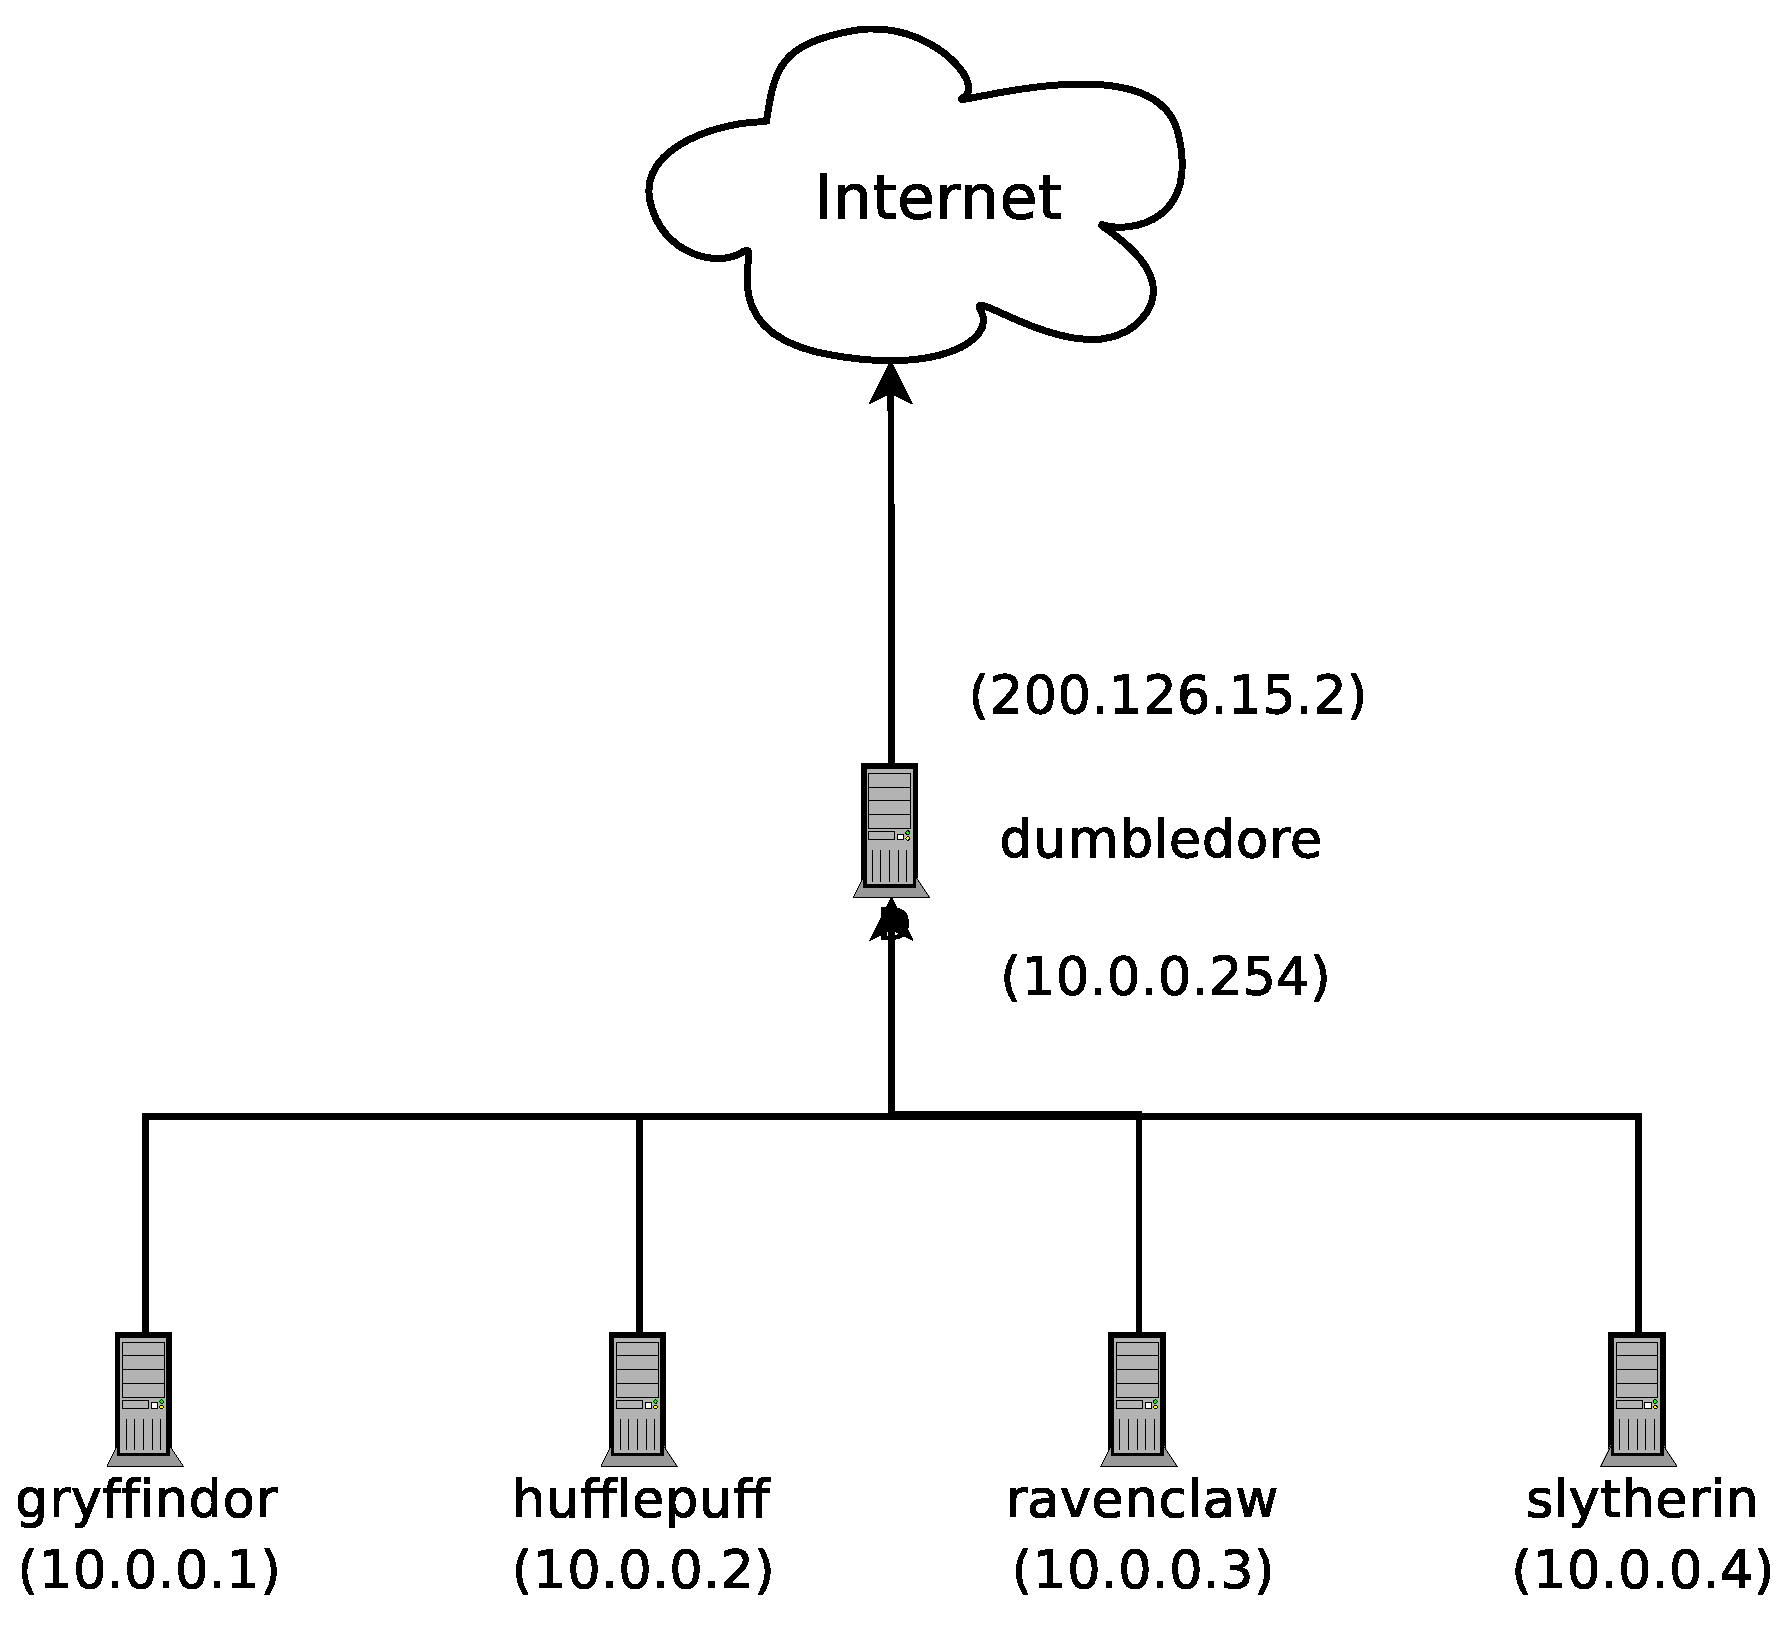
\includegraphics[scale=.5]{HogwartsNet}
\caption{Rede exemplo \texttt{hogwarts}}
\label{fig:nethogwarts}
\end{figure}

No caso, imaginemos que  voc� est� configurando inicialmente a m�quina
\texttt{hufflepuff}.  Como  \texttt{root},   voc�  dever�  utilizar  o
comando:

\begin{center}
\begin{verbatim}
ifconfig eth0 10.0.0.2 netmask 255.0.0.0 broadcast 10.0.0.255 up
\end{verbatim}
\end{center}

Perceba que falamos que ele utiliza o \emph{netmask} padr�o para a sua
Classe IP. Al�m  disso, em geral o \emph{broadcast}  pode ser definido
conforme a necessidade pelo \texttt{ifconifg}. Nesse caso, se desejar,
voc� pode definir a interface com o seguinte comando.

\begin{center}
\begin{verbatim}
ifconfig eth0 10.0.0.2 up
\end{verbatim}
\end{center}

Al�m   disso   normalmente    o   \texttt{ifconfig}   j�   conseguiria
automaticamente  estabelecer um  roteamento  de rede  normal. Se  voc�
preferir,  sempre  pode-se  usar  \texttt{route} para  estabelecer  um
roteamento manual,  sendo que isso � �til  principalmente para pacotes
IPs para \emph{fora} da rede  interna (por exemplo, para a Internet ou
para uma  VPN\footnote{\emph{Virtual Private Network}  -- Rede Privada
Virtual}). Por  exemplo, imaginando que queremos  estabelecer uma rota
padr�o por  \texttt{dumbledore} para \emph{todos} os  pacotes da rede,
usamos o comando:

\begin{center}
\begin{verbatim}
route add default gw 10.0.0.254
\end{verbatim}
\end{center}

O  pr�prio  \texttt{route} se  configura:  o  \emph{The Linux  Network
Administrators'   Guide,  Second  Edition},   de  \citeonline{NAG2000}
explica que o  \emph{kernel} do Linux checa a  tabela de interfaces de
rede  configuradas, de modo  a rotear  para uma  interface configurada
para mandar os pacotes de um  IP parte da mesma rede do \emph{gateway}
e define essa interface como a interface de sa�da dos dados.

\section{Arquivos de informa��es sobre redes}

Como  voc�   deve  ter  notado,  trabalhamos  muito   com  n�meros  de
IPs. Por�m, embora IPs sejam  fundamentais para o funcionamento de uma
rede, �  muito dif�cil  para uma  pessoa comum decorar  os IPs  de uma
rede, exceto por redes  pequenas e triviais, o que \emph{dificilmente}
� a  realidade de um  ambiente de redes tradicional,  onde normalmente
temos  uma grande quantidade  de IPs  para os  mais diversos  tipos de
recursos e  m�quinas, tanto \emph{hosts} quanto  terminais.  Por isso,
diversos  esquemas   de  criar-se  nomes  simples   de  m�quina  foram
desenvolvidos com o tempo. 

Embora existam  esquemas como DNS\footnote{\emph{Domain  Name Service}
  -- Servi�o de  Nomes de Dom�nio}  e DDNS\footnote{\emph{Dynamic DNS}
  -- DNS din�mico}(tamb�m conhecido como \emph{Bonjour}), em redes n�o
muito grandes, principalmente redes internas, pode-se adotar o esquema
tradicional por  arquivos do  Linux. Esse esquema  envolve basicamente
quatro    arquivos:    \texttt{/etc/hosts},    \texttt{/etc/networks},
\texttt{/etc/HOSTNAME} e \texttt{/etc/resolv.conf}.

\subsection{\texttt{/etc/HOSTNAME}}

O arquivo \texttt{/etc/HOSTNAME}  permite configurar-se o nome interno
da m�quina.  Isso  � muito �til em alguns casos,  mas nas vers�es mais
atuais do Linux o uso  do \texttt{/etc/HOSTNAME} vem caindo por terra,
na realidade o \texttt{/etc/HOSTNAME} contem apenas uma linha, como no
caso   do    Trecho   de   C�digo    \ref{fig:hostname},   na   P�gina
\pageref{fig:hostname}. O  primeiro nome � o nome  simples da m�quina,
acess�vel a todos os usu�rios da rede em quest�o, enquanto o segundo �
um FQDN\footnote{\emph{Fully Qualified Domain Name} -- Nome de Dom�nio
Totalmente  Descrito} da  m�quina em  quest�o.  Normalmente  ele seria
alguma coisa  do tipo \texttt{www.google.com},  mas, principalmente em
m�quinas  em  intranets, nada  impede  que se  adote  um  FQDN como  o
descrito anteriormente, ou seja, \texttt{hufflepuff.hogwarts}.

\begin{codigo}
\begin{center}
\begin{verbatim}
hufflepuff      hufflepuff.hogwarts
\end{verbatim}
\caption{Exemplo de \texttt{/etc/HOSTNAME}}
\label{fig:hostname}
\end{center}
\end{codigo}

Nas  vers�es  mais  atuais   do  \emph{kernel}  do  Linux,  o  arquivo
\texttt{/etc/HOSTNAME} acabou caindo  por terra, sendo substituido por
uma  combina��o  do comando  \texttt{hostname}  (para configura��o  em
\emph{runtime})  e do  arquivo \texttt{/etc/hosts}  (para configura��o
persistente). 

\subsection{\texttt{/etc/hosts}}

Na verdade, o \texttt{/etc/hosts} � o arquivo que contem as defini��es
dos nomes de \emph{hosts} de uma  rede. Sua origem remonta a origem da
Internet,   quando   um   arquivo   \emph{hosts}  era   mantido   pela
IANA\footnote{\emph{Internet Assigned Names  and Addresses} -- Nomes e
  Endere�os  distribu�dos  pela  Internet:  organiza��o que  mant�m  a
  distribui��o  dos IPs  de  uma rede}  e  redistribu�do conforme  era
atualizado na Internet. Com o tempo, esse esquema deu lugar a esquemas
como o  DNS, mas  sua utilidade  para redes de  porte pequeno  a m�dio
continuou bastante v�lida. 

O arquivo  \texttt{/etc/hosts} �  similar em funcionamento  ao arquivo
\texttt{/etc/HOSTNAME}, mas com uma linha por IP.  Al�m disso, cada IP
pode  ter,  al�m  dos  nomes  de  m�quina  e  dos  FQDN,  um  ou  mais
\emph{alias} (apelidos) para as  mesmas estabelecidos. Por exemplo, na
Trecho de C�digo  \ref{fig:hosts}, P�gina \pageref{fig:hosts}, vemos a
lista   de  \emph{hosts}   da  Figura   \ref{fig:nethogwarts},  P�gina
\pageref{fig:nethogwarts}. Al�m  isso, cada dom�nio possui  um ou mais
\emph{alias}, como  o caso, por exemplo, de  \texttt{supercomp}, que �
um \emph{alias} para \texttt{hufflepuff}.

\begin{codigo}
\begin{center}
\begin{verbatim}
127.0.0.1     localhost localhost.localdomain
10.0.0.1      gryffindor gryffindor.hogwarts security security.hogwarts
10.0.0.2      hufflepuff hufflepuff.hogwarts supercomp supercomp.hogwarts
10.0.0.3      ravenclaw ravenclaw.hogwarts data data.hogwarts
10.0.0.4      slytherin slytherin.hogwarts cert cert.hogwarts
10.0.0.254    dumbledore dumbledore.hogwarts proxy proxy.hogwarts
\end{verbatim}
\caption{Exemplo de \texttt{/etc/hosts}}
\label{fig:hosts}
\end{center}
\end{codigo}

Algumas   instala��es  ou   administradores   preferem  separar   cada
\emph{alias} e  FQDN por linha, repetindo  o IP na  primeira coluna do
arquivo.     O    Trecho    de   C�digo    \ref{fig:hosts2},    P�gina
\pageref{fig:hosts2},  apresenta  um  exemplo  de  \texttt{/etc/hosts}
dividido por linha como o exemplo do Trecho de C�digo \ref{fig:hosts},
P�gina  \pageref{fig:hosts}.  Essa  disposi��o �  heran�a  dos padr�es
antigos  do Unix\texttrademark,  e continua  sendo usado  no Microsoft
Windows\texttrademark.  A  ado��o desse padr�o nos  Unix mais modernos
no Linux  fica a crit�rio  do administrador do sistema,  conforme suas
necessidade. Pode-se  inclusive usar uma vers�o separando  os nomes de
m�quinas  e  os de  \emph{alias}  Trecho  de C�digo  \ref{fig:hosts3},
P�gina \pageref{fig:hosts3}.  O esquema  a ser adotado fica a crit�rio
do pr�prio  desenvolvedor.  De qualquer forma, uma  sugest�o � colocar
coment�rios (que come�am com \texttt{\#}) explicando seu padr�o.

\begin{codigo}
\begin{ttfamily}
127.0.0.1     localhost localhost.localdomain

10.0.0.1      gryffindor 

10.0.0.1      gryffindor.hogwarts 

10.0.0.1      security 

10.0.0.1      security.hogwarts

\vdots

10.0.0.254    dumbledore 

10.0.0.254    dumbledore.hogwarts 

10.0.0.254    proxy 

10.0.0.254    proxy.hogwarts
\end{ttfamily}
\begin{center}
\caption{Exemplo de \texttt{/etc/hosts} separado por linhas}
\label{fig:hosts2}
\end{center}
\end{codigo}

\begin{codigo}
\begin{center}
\begin{verbatim}
127.0.0.1     localhost localhost.localdomain
10.0.0.1      gryffindor gryffindor.hogwarts 
10.0.0.1      security security.hogwarts
10.0.0.2      hufflepuff hufflepuff.hogwarts
10.0.0.2      supercomp supercomp.hogwarts
10.0.0.3      ravenclaw ravenclaw.hogwarts
10.0.0.3      data data.hogwarts
10.0.0.4      slytherin slytherin.hogwarts 
10.0.0.4      cert cert.hogwarts
10.0.0.254    dumbledore dumbledore.hogwarts 
10.0.0.254    proxy proxy.hogwarts
\end{verbatim}
\caption{Exemplo de \texttt{/etc/hosts} separando nomes de m�quina e \emph{aliases}}
\label{fig:hosts3}
\end{center}
\end{codigo}

Perceba,  por  fim,  que  em  \emph{todos}  os  exemplos,  existe  uma
defini��o  para  o \emph{localhost}.  Isso  �  importante pois  alguns
servi�os,  como  a  interface  gr�fica  X,  dependem  de  uma  entrada
\emph{localhost} para localizar corretamente  os servidores e dados na
m�quina   local.   Nunca,  \emph{jamais},   apague   a  defini��o   do
\emph{localhost},  ou crie  um \texttt{/etc/hosts}  sem a  mesma, pois
isso pode resultar em problemas de comportamento do sistema. 

\subsection{\texttt{/etc/networks}}

\texttt{/etc/networks} auxilia  a administra��o  das redes �s  quais o
sistema pode acessar diretamente, assim  como ao nomeamento de redes e
equipamentos.  Seu  principal  uso   �  facilitar  o  uso  do  comando
\texttt{route}, ao desobrigar o administrador de decorar IPs de rede. 


\begin{figure}
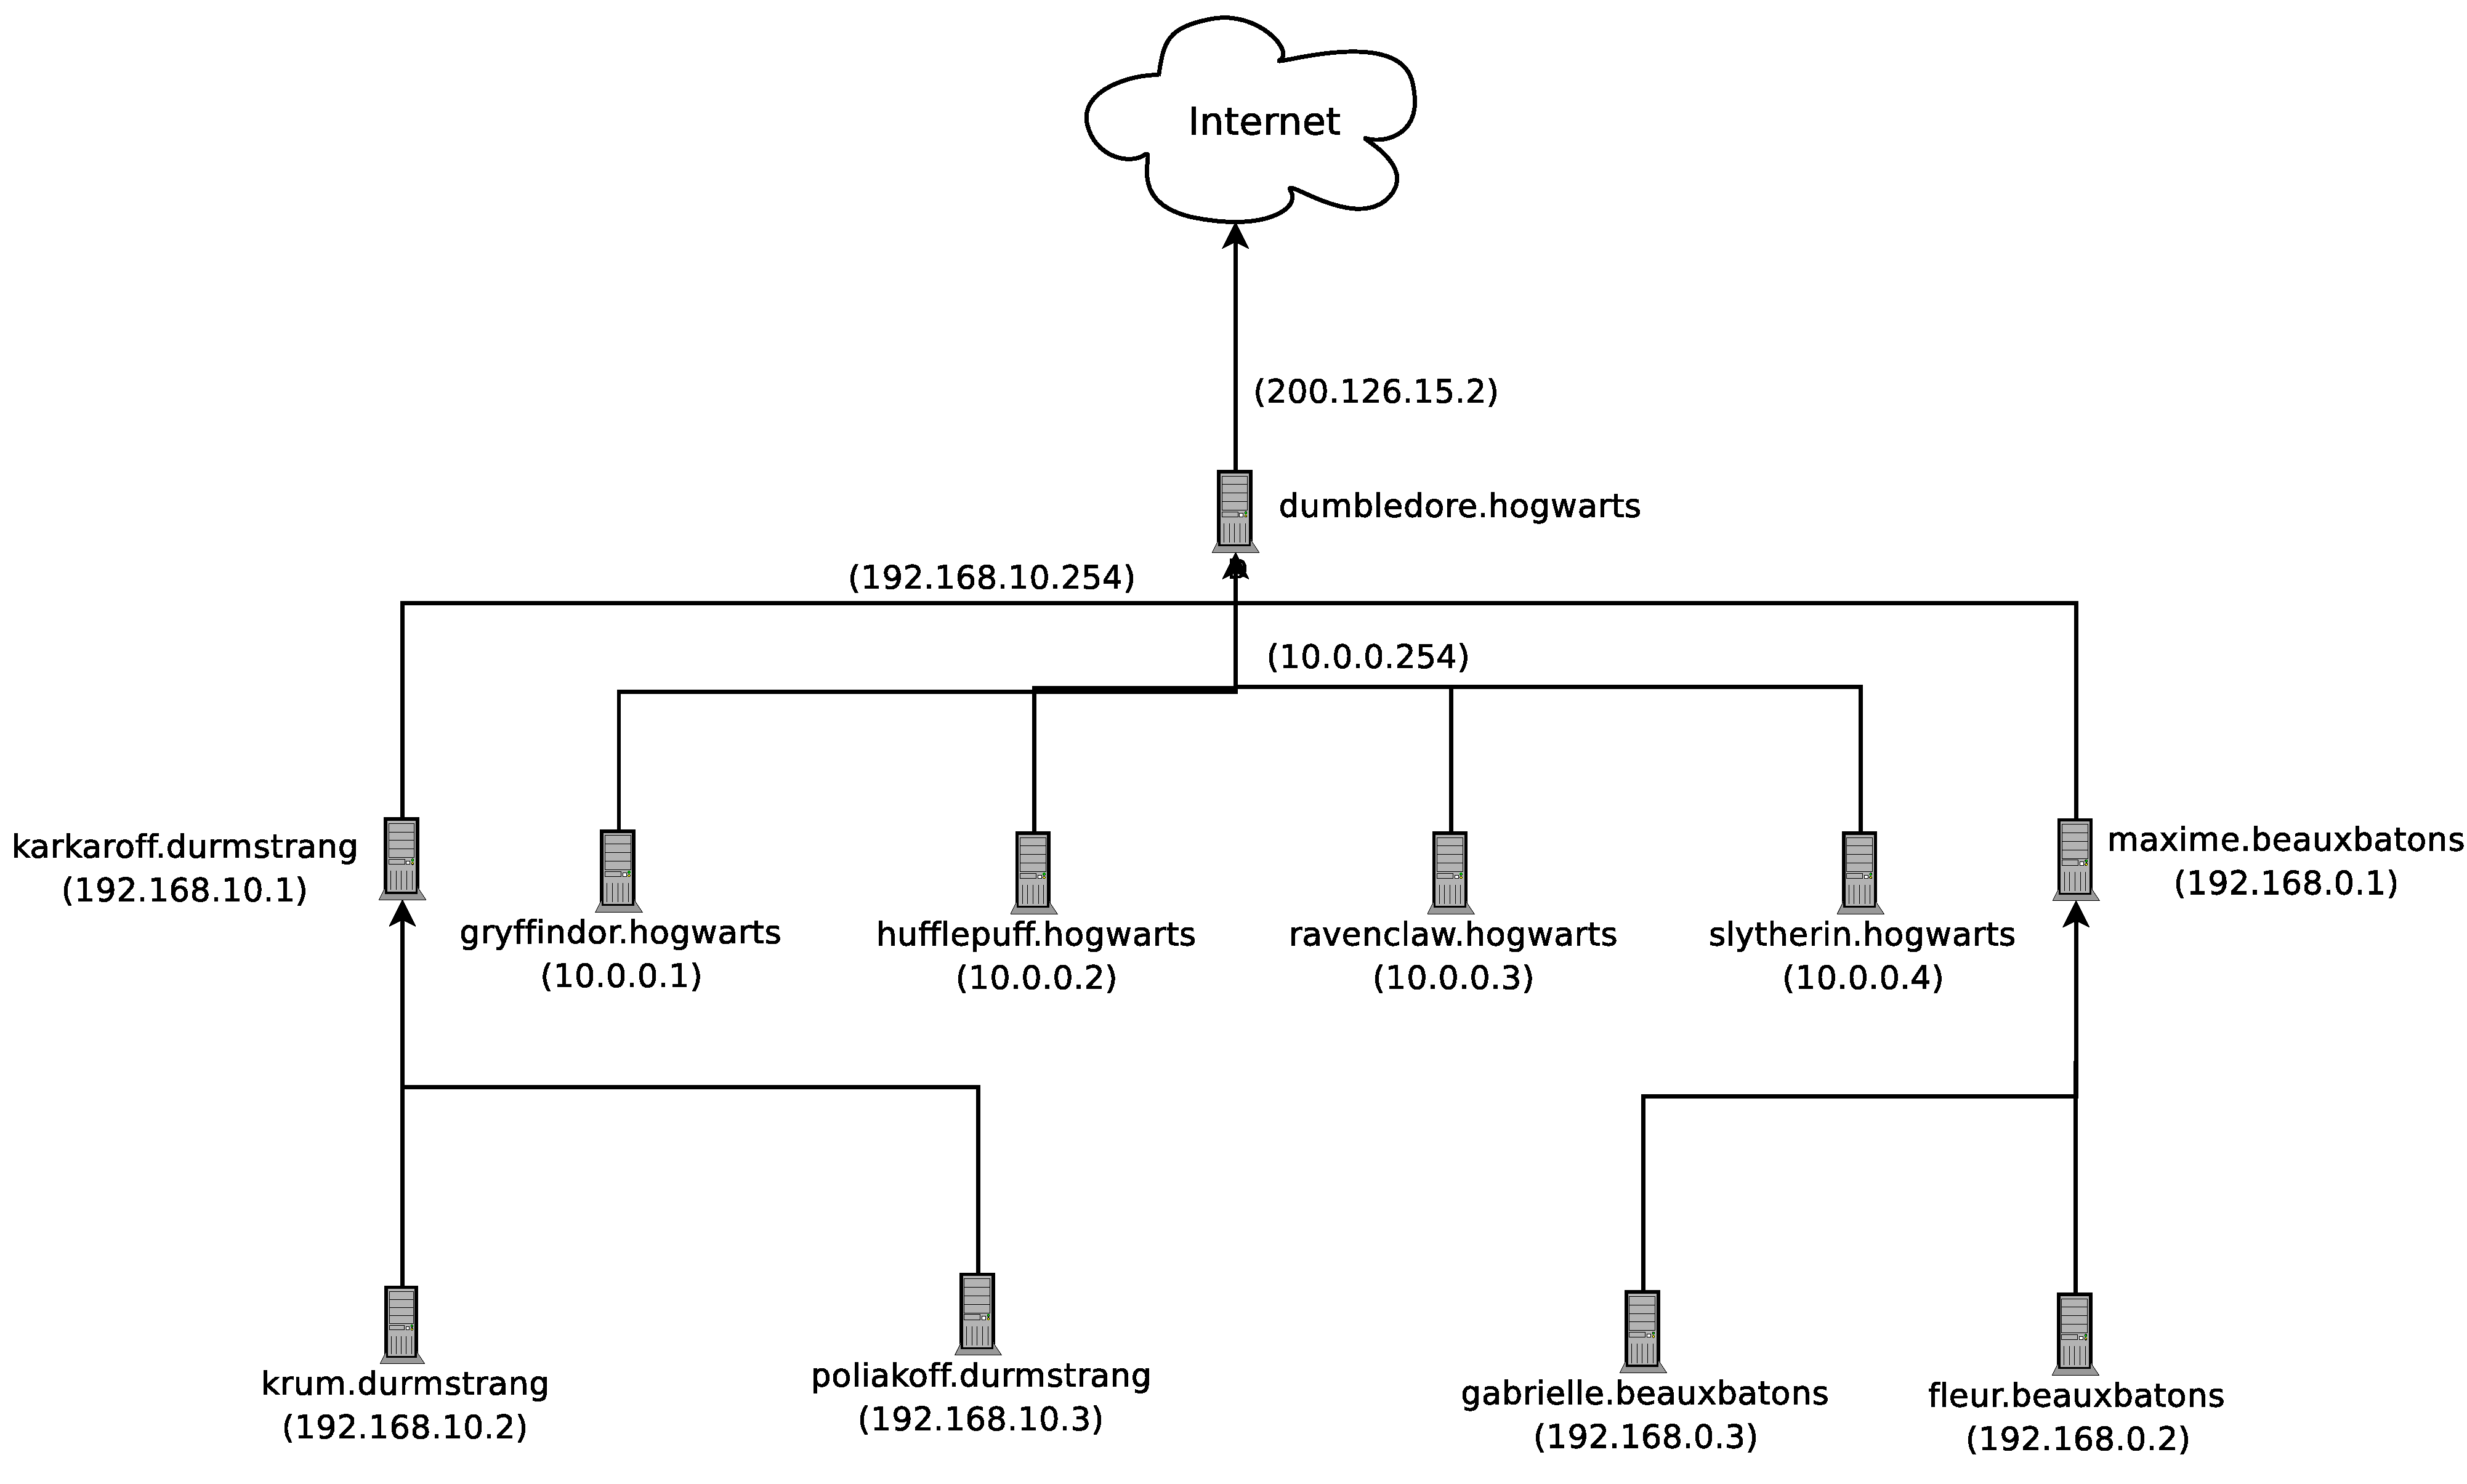
\includegraphics[angle=90,scale=.33]{HogwartsNet2}
\caption{Redes exemplo \texttt{hogwarts}, \texttt{durmstrang} e \texttt{beauxbatons}}
\label{fig:nethogwarts2}
\end{figure}

Vejamos agora um exemplo que nos auxilie a entender: imaginemos a rede
da  Figura  \ref{fig:nethogwarts} (P�gina  \pageref{fig:nethogwarts}).
Agora,  imaginemos  que  a  rede  \texttt{hogwarts}  comece  a  prover
servi�os    para   duas    outras   redes,    \texttt{beauxbatons}   e
\texttt{durmstrang},      conforme      apresentado     na      Figura
\ref{fig:nethogwarts2} (P�gina  \pageref{fig:nethogwarts2}). Como voc�
pode perceber, as  m�quinas \texttt{durmstrang} e \texttt{beauxbatons}
n�o possuem  acesso via Internet  direto, precisando passar  pela rede
\texttt{hogwarts}.   Para isso,  � necess�rio  fazer o  roteamento dos
pacotes     IPs     de    suas     redes     atrav�s    da     m�quina
\texttt{dumbledore.hogwarts}.   Para isso,  tem que  editar  o arquivo
\texttt{/etc/networks} e configurar corretamente as redes. Em todos as
esta��es   com  roteamento   (no   caso  \texttt{dumbledore.hogwarts},
\texttt{maxime.beauxbatons},  \texttt{karkaroff.durmstrang}) o arquivo
\texttt{/etc/network}  dever� ser  definido como  no Trecho  de C�digo
\ref{fig:network}, P�gina \pageref{fig:network}

\begin{codigo}
\begin{center}
\begin{verbatim}
hogwarts          10.0.0.0
beauxbatons    192.168.0.0
durmstrang    192.168.10.0
\end{verbatim}
\caption{Exemplo de \texttt{/etc/network} para a rede da Figura \ref{fig:nethogwarts2}}
\label{fig:network}
\end{center}
\end{codigo}

Bem,  voc�  deve  estar  perguntando \emph{``qual  a  diferen�a  nisso
tudo??''}.    Na    verdade,   da   mesma   forma    que   o   arquivo
\texttt{/etc/hosts},  o \texttt{/etc/network} auxilia  na configura��o
de  rede  por comandos.  No  caso,  ele  facilita a  configura��o  via
\texttt{route}.  No  caso, ambas as  redes podem ser  configuradas por
meio do comando \texttt{route add default gateway dumbledore.hogwarts}
e  \texttt{route   add  -net  beauxbatons}(por   exemplo,  na  m�quina
\texttt{fleur.beauxbatons}). 

Na verdade, existem sempre os  mecanismos de DNS que podem valer muito
mais a pena,  mas esse sistema, para redes pequenas  e m�dias deve ser
mais do que o suficiente. 

\begin{codigo}
\begin{center}
\begin{verbatim}
127.0.0.1     localhost localhost.localdomain
10.0.0.1      gryffindor gryffindor.hogwarts 
10.0.0.2      hufflepuff hufflepuff.hogwarts
10.0.0.3      ravenclaw ravenclaw.hogwarts
10.0.0.4      slytherin slytherin.hogwarts 
10.0.0.254    dumbledore dumbledore.hogwarts 
192.168.10.1  karkaroff karkaroff.durmstrang
192.168.10.2  krum krum.durmstrang
192.168.10.3  poliakoff poliakoff.durmstrang
192.168.0.1   maxime maxime.beauxbatons
192.168.0.2   fleur fleur.beauxbatons
192.168.0.3   gabrielle gabrielle.beauxbatons
\end{verbatim}
\caption{Exemplo de \texttt{/etc/hosts} para a rede da Figura \ref{fig:nethogwarts2}}
\label{fig:hosts4}
\end{center}
\end{codigo}

\begin{quotation}
  \textbf{Nota:} como  conselho, cada m�quina conectada  a um ambiente
  como  o  da  Figura  \ref{fig:nethogwarts2},  deve  ter  um  arquivo
  \texttt{/etc/hosts}  como  o do  Trecho  de C�digo  \ref{fig:hosts4}
  (P�gina  \pageref{fig:hosts4}), para que  o mesmo  consiga localizar
  corretamente todas as m�quinas.
\end{quotation}

\section{Arquivos de \emph{resolver}}

Uma parte  importante das funcionalidades  de rede do Linux  involve o
\emph{resolver}.  Esse componente  interno ao  \emph{kernel}  do Linux
permite que  o sistema resolva  os nomes de  m�quina, ou seja,  fa�a a
convers�o do nome de m�quina ou do FQDN para IPs. 

Como  foi  dito, os  nomes  de  m�quina/\emph{alias}/FQDNs s�o  apenas
formas  de tornar  ao  usu�rio mais  simples  o acesso  a m�quinas  ou
recursos  da mesma.  Para o  computador, ele  \emph{continua  usando o
  IP}.  Esse  entendimento  ajuda   a  compreender  a  import�ncia  do
\emph{resolver}.  Na pr�tica, ele  utiliza todos  os mecanismos  que o
\emph{kernel}  conhecer para \emph{resolver  o IP},  ou seja,  pegar o
nome fornecido pela aplica��o  do usu�rio, ``traduzir'' esse nome para
um valor  de IP que  o sistema possa  usar na transmiss�o via  rede, e
us�-lo para  conectar a m�quina  cliente ao \emph{host} com  o servi�o
desejado. 

Para  configurar  como o  \emph{resolver}  do  ambiente  Linux ir�  se
comportar,  s�o usados  dois arquivos,  o \texttt{/etc/host.conf}  e o
\texttt{/etc/resolv.conf}.

\subsection{O arquivo \texttt{/etc/host.conf}}

O  arquivo   \texttt{/etc/host.conf}  configura  o   comportamento  do
\emph{resolver}. Em  geral ele  vai ter apenas  algumas configura��es,
sempre linha por linha. 

A primeira op��o � \texttt{order}, que configura a seq��ncia na qual o
\emph{resolver} tentar� resolver  o nome de m�quina passado  a ele. Os
valores dele s�o:

\begin{itemize}
  \item  \texttt{bind} ---  esse par�metro  indica que  o  sistema ir�
    recorrer ao sistema de DNS para resolver o nome de m�quina;
  \item  \texttt{hosts}  --- esse  par�metro  faz  com  que o  sistema
    utilize o esquema tradicional,  que � atrav�s dos arquivos citados
    anteriormente, como \texttt{/etc/hosts} e \texttt{/etc/network};
  \item \texttt{nis} --- esse  par�metro permite que o sistema resolva
    o nome  de m�quina pelo sistema de  NIS (\emph{Network Information
    Service}   --  Servi�o   de  Informa��o   de  Rede),   um  sistema
    originalmente da  Sun Microsystems que  � muito usado  em ambiente
    exclusivamente Unix, como no caso de redes \emph{cluster}, por sua
    simplicidade e leveza comparada com outros sistemas;
\end{itemize}

Essa op��o n�o  possui valor �nico, podendo ser  inseridas todas essas
op��es sem problemas. No caso, cada op��o deve ser separada das demais
com  uma v�rgula, como  no caso  de \texttt{order  bind, hosts},  e as
op��es devem ser colocadas na seq��ncia de prioridade � qual o sistema
ir�  recorrer na  resolu��o  do  nome. Nesse  exemplo,  o sistema  ir�
recorrer  primeiro ao  DNS  e  em seguida  ao  sistema tradicional  de
arquivos do Unix.

Outra  op��o  importante  �  \texttt{multi}, aonde  o  \emph{resolver}
responde �  requisi��o do sistema recuperando  \emph{todos} os valores
IP que  ele puder  resolver para o  nome de m�quina  oferecido. Embora
isso  ocasionalmente possa  provocar conflitos,  �  muito interessante
manter em \texttt{on} permitindo, por  exemplo, que no caso de mudan�a
de IP n�o aja problemas na resolu��o de um \emph{site}. Agora, no caso
de ambientes  internos simples,  pode ser interessante  desativar essa
op��o com \texttt{off}. 

Uma op��o de seguran�a na resolu��o de IP � \texttt{nospoof}. Ativando
essa  op��o  em  \texttt{on},   o  sistema  ir�,  ap�s  uma  resolu��o
(principalmente   para   \emph{remote   shell},   \texttt{telnet},   e
\emph{secure   shell})  execut�-la  novamente.    Se  os   valores  de
\emph{ambas} as  resolu��es n�o casarem, isso  significa uma tentativa
de       \emph{spoof}      por      t�cnicas       como      \emph{DNS
poisoning}\footnote{\emph{DNS poisoning}  � uma t�cnica  que envolve a
substitui��o de  valores DNS  leg�timos por valores  falsificados, por
meio de substitui��es na seq��ncia  em que os servidores s�o chamados,
literalmente  ``envenenando''  o \emph{cache}  de  DNS  do sistema}  e
similares,  o que  o  sistema ir�  automaticamente ``cortar''.  Por�m,
saiba que isso com certeza  ir� reduzir a performance do sistema, pois
ele  dever�  realizar   \emph{duas}  resolu��es  de  nome  \textbf{por
  vez}. Portanto, use com cautela essa op��o.

A op��o anterior  pode ter seu n�vel de  seguran�a ampliado ainda mais
por meio de outra op��o, que � a op��o \texttt{spoofalert}, tamb�m com
valores \texttt{on} e \texttt{off}. No caso, se \emph{ambas} as op��es
\texttt{nospoof}    e     \texttt{spoofalert}    estiverem    ativadas
(\texttt{on}), uma mensagem de erro do \emph{resolver} ser� enviada ao
\emph{syslog}, o registro de informa��es (\emph{log}) do sistema. Para
mais   informa��es   sobre   o   \emph{syslog},   consulte   a   Se��o
\ref{sec:syslog}, na P�gina \pageref{sec:syslog}.

Isso deve  ser o suficiente sobre  \texttt{/etc/host.conf}. Um exemplo
desse   arquivo   pode   ser    encontrado   no   Trecho   de   C�digo
\ref{fig:hostsconf}, P�gina \pageref{fig:hostsconf}.

\begin{codigo}
\begin{center}
\begin{verbatim}
order hosts,bind
multi on
\end{verbatim}
\caption{Exemplo de \texttt{/etc/hosts.conf}}
\label{fig:hostsconf}
\end{center}
\end{codigo}

\subsection{O arquivo \texttt{/etc/resolv.conf}}

O  segundo  arquivo  que  podemos  dizer  que  �  de  configura��o  do
\emph{resolver}  � o  \texttt{/etc/resolv.conf}. Esse  arquivo permite
configurar corretamente o \emph{resolver} em como ele ir� se comportar
no  caso das  op��es estabelecidas  no  \texttt{/etc/hosts.conf}.  Ele
armazena  informa��es  sobre  quais  servidores de  nome  dever�o  ser
procurados  e em que  seq��ncia. Perceba  que quando  � usado  o termo
servidor   de  nome   (\emph{nameserver})  nesse   arquivo,  \emph{n�o
diferenciariamos} servidores de nome dos diversos modelos, como NIS ou
DNS.  A  responsabilidade quanto a  isso deve ser  do \emph{resolver},
baseando-se no esquema definido no arquivo \texttt{/etc/hosts.conf}.

�  importante deixar claro  que \emph{n�o  � necess�rio}  configurar o
\emph{resolver}  em uma  m�quina  que  tenha um  servidor  DNS ou  NIS
pr�prio rodando, ou que ainda  necessite apenas de informa��es de nome
de \emph{hosts} em rede vindas do \texttt{/etc/hosts}.  A configura��o
do  \emph{resolver}  s� �  necess�ria  se  o  sistema precisar  buscar
servidores  de   nome  remotos.  Se   um  servidor  de   nome  estiver
configurado,  o \emph{resolver}  poder� ser  desativado,  deixando por
conta  do servidor  de nomes  local da  m�quina a  responsabilidade de
resolver o  nome de  m�quina ao servidor  local. Isso s�  � necess�rio
quando um sistema precisar de um  servidor de nomes remoto, como em um
\emph{desktop} conectada � Internet sem nenhum servidor de nomes local
ativo.

O   \texttt{/etc/resolv.conf}  �  constru�do   de  forma   similar  ao
\texttt{/etc/hosts.conf}, ou seja, com uma op��o por linha de texto no
arquivo. Suas principais op��es s�o:

\begin{itemize}
  \item \textbf{\texttt{nameserver:}} essa  op��o permite configurar o
    IP  de uma  m�quina remota  que servir�  a resolu��o  de  nomes de
    m�quina. Perceba que \emph{n�o � necess�rio determinar qual o tipo
    de sistema de nome adotado}, NIS, DNS ou qualquer outro. Isso fica
    a cargo do pr�prio \emph{resolver} determinar;
  \item  \textbf{\texttt{domain:}} essa  op��o ajuda  a  identificar o
    dom�nio ao qual  a m�quina configurada pertence, de  maneira que o
    sistema   de  consulta   de  nome   de  dom�nio   possa  trabalhar
    adequadamente  na  resolu��o  de  nomes curtos  ou  \emph{aliases}
    passados.    Isso  �   feito  por   meio  da   expans�o   do  nome
    curto/\emph{alias} para o FQDN apropriado. Por exemplo, imaginemos
    que  a m�quina  \texttt{fleur} do  arquivo  \texttt{/etc/hosts} do
    Trecho  de C�digo  \ref{fig:hosts4}  (P�gina \pageref{fig:hosts4})
    esteja buscando o servidor \texttt{hufflepuff.hogwarts}.  Ela pode
    utilizar o  nome curto \texttt{hufflepuff},  mas o \emph{resolver}
    em sua m�quina est�  configurado para ``expandir'' os nomes curtos
    de m�quina usando \texttt{beauxbatons}  como nome curto.  No caso,
    o primeiro servidor que ela ir� procurar ser� o ``expandido'', que
    ser� determinado  como \texttt{hufflepuff.beauxbatons}.  Como essa
    m�quina n�o existe, ele tentar� localizar \texttt{hufflepuff}, sem
    nenhum nome de dom�nio. Essa  m�quina tamb�m n�o existe, o que ir�
    provocar a falha na pesquisa.

    Essa  op��o  pode  receber   at�  seis  dom�nios  diferentes  para
  ``expans�o'' dos nomes curtos e \emph{aliases} oferecidos, sendo que
    o n�mero  de caracteres nessas seis op��es  \emph{juntas} n�o pode
    superar 256 caracteres.
\end{itemize}

\begin{codigo}
\begin{center}
\begin{verbatim}
nameserver 200.167.20.5
nameserver 200.176.2.10
# nameserver 192.168.20.2

# ppp temp entry
\end{verbatim}
\caption{Exemplo de \texttt{/etc/resolv.conf}}
\label{fig:resolvconf}
\end{center}
\end{codigo}

Existem   outras  tantas   op��es,  que   podem  ser   consultadas  na
\emph{manpage}   \texttt{resolv.conf}(8).     O   Trecho   de   C�digo
\ref{fig:resolvconf}, na P�gina \pageref{fig:resolvconf}, apresenta um
exemplo de configura��o de \texttt{/etc/resolv.conf}.

\section{\sloppy{O  arquivo   \texttt{/etc/rc.d/init.d/network}  e  o  arquivo
  \texttt{/etc/sysconfig/network}}}

\fussy

Uma  pergunta que deve  estar passando  por sua  cabe�a �  ``tudo bem,
entendi tudo  isso. Mas como a  m�quina sabe qual �  a configura��o de
rede que ele deve ter?''

Na  realidade,   como  na   maioria  dos  sistemas   operacionais,  as
configura��es  no Linux  s�o \emph{transientes},  ou seja,  elas est�o
ativas enquanto  o sistema estiver no  ar. Uma vez que  o sistema seja
retirado do ar, as configura��es desaparecem. 

Isso  parece uma  tolice, mas  a realidade  � que  o  funcionamento da
maioria dos  sistemas �  esse. Por�m, assim  como outros  sistemas com
essa  caracter�stica,  o Linux  oferece  um  mecanismo  que permite  a
perman�ncia  dessas  configura��es. No  caso,  a  maioria das  distros
GNU/Linux  possuem  algum  tipo  de \emph{shell  script}  que  permite
carregar  e  configurar  as  informa��es  das interfaces  de  rede  no
\emph{boot} da  m�quina.  Nos  sistemas baseados em  System V  Unix (a
grande         maioria),        esse        arquivo         �        o
\texttt{/etc/rc.d/init.d/network}.  Em  outras  distros,  baseadas  no
modelo    BSD     (como    o    Slackware),    o     arquivo    �    o
\texttt{/etc/rc.d/rc.inet1}. Veremos  mais sobre os  v�rios modelos de
inicializa��o na Se��o \ref{cap:sysv}, P�gina \pageref{cap:sysv}. 

No caso, n�o h� muito a se  dizer sobre o arquivo em quest�o: ele � um
\emph{shell  script}  pr�-constru�do   de  f�brica,  que  permite  sua
configura��o por  outros caminhos. A t�tulo de  configura��o, o Trecho
de   C�digo  \ref{fig:rcdnetwork}  a   \ref{fig:rcdnetwork6},  P�ginas
\pageref{fig:rcdnetwork}  a   \pageref{fig:rcdnetwork6},  apresenta  o
\texttt{/etc/rc.d/init.d/network}   da  distribui��o   Mandriva  Linux
2006.0 Free. 

\begin{codigo}
\begin{center}
\begin{scriptsize}
\begin{verbatim}
#! /bin/bash
#
# network       Bring up/down networking
#
# chkconfig: 2345 10 90
# description: Activates/Deactivates all network interfaces configured to \
#              start at boot time.
# probe: false
### BEGIN INIT INFO
# Provides: $network
### END INIT INFO

# Source function library.
. /etc/init.d/functions

if [ ! -f /etc/sysconfig/network ]; then
    echo "NETWORKING=no" > /etc/sysconfig/network
    exit 0
fi

. /etc/sysconfig/network

if [ -f /etc/sysconfig/pcmcia ]; then
	. /etc/sysconfig/pcmcia
fi


# Check that networking is up.
[ "${NETWORKING}" = "no" ] && exit 0

# if the ip configuration utility isn't around we can't function.
[ -x /sbin/ip ] || exit 1

# Even if IPX is configured, without the utilities we can't do much
[ ! -x /sbin/ipx_internal_net -o ! -x /sbin/ipx_configure ] && IPX=

# Even if VLAN is configured, without the utility we can't do much
[ ! -x /sbin/vconfig ] && VLAN=

# If IPv6 is explicitly configured, make sure it's available.
if [ -n "$NETWORKING_IPV6" ]; then
    alias=`modprobe -c | awk '/^alias net-pf-10 / { print $3; exit }'`
    if [ "$NETWORKING_IPV6" = "yes" ]; then
	new_alias=ipv6
    fi
    if [ "$NETWORKING_IPV6" = "no" ]; then
	new_alias=off
    fi
    if [ -n "$new_alias" ]; then
	if [ "$alias" != "$new_alias" -a ! -f /proc/net/if_inet6 ]; then
		case "$(modprobe -V 2>/dev/null)" in
			modprobe* )
				echo "alias net-pf-10 $new_alias" >> /etc/modules.conf
			;;
			module-init-tools* )
				echo "alias net-pf-10 $new_alias" >> /etc/modprobe.conf
			;;
		esac
	fi
    fi
fi

\end{verbatim}
\end{scriptsize}
\caption{Exemplo de \texttt{/etc/rc.d/init.d/network}}
\label{fig:rcdnetwork}
\end{center}
\end{codigo}

\begin{codigo}
\begin{center}
\begin{scriptsize}
\begin{verbatim}
CWD=`pwd`
cd /etc/sysconfig/network-scripts

. network-functions

# find all the interfaces besides loopback.
# ignore aliases, alternative configurations, and editor backup files
interfaces=`ls ifcfg* | LANG=C egrep -v '(ifcfg-lo|:|rpmsave|rpmorig|rpmnew)' | \
	    LANG=C egrep -v '(~|\.bak)$' | \
            LANG=C egrep 'ifcfg-[A-Za-z0-9\._-]+$' | \
            sed 's/^ifcfg-//g' |
            sed 's/[0-9]/ &/' | LANG=C sort -k 1,1 -k 2n | sed 's/ //'`

boot=boot

# See how we were called.
case "$1" in
  start)
	# IPv6 hook (pre IPv4 start)
	if [ "$NETWORKING_IPV6" = "yes" ]; then
		if [ -x /etc/sysconfig/network-scripts/init.ipv6-global ]; then
			/etc/sysconfig/network-scripts/init.ipv6-global start pre
		fi
	fi
  
  	action "Setting network parameters: " sysctl -e -p /etc/sysctl.conf

	if [ -r /etc/ethers -a -x /sbin/arp ]; then
	    action "Storing ARP mapping" /sbin/arp -f /etc/ethers
	fi
	
	# bring up loopback interface
	action "Bringing up loopback interface: " ./ifup ifcfg-lo

	case "$IPX" in
	  yes|true)
	    /sbin/ipx_configure --auto_primary=$IPXAUTOPRIMARY \
				   --auto_interface=$IPXAUTOFRAME
	    if [ "$IPXINTERNALNETNUM" != "0" ]; then
	       /sbin/ipx_internal_net add $IPXINTERNALNETNUM $IPXINTERNALNODENUM
	    fi
	    ;;
	esac
	# depreciated but we still use it.
	if [ -f /proc/sys/net/ipv4/ip_forward ] && [[ "$FORWARD_IPV4" = "yes" || "$FORWARD_IPV4" = "true" ]]; 
	    then
		action "Enabling IPv4 packet forwarding" sysctl -n -w net.ipv4.ip_forward=1
	fi

	case "$VLAN" in
	  yes)
	    if [ -d /proc/net/vlan ] || modprobe 8021q >/dev/null 2>&1 ; then
		action "Setting 802.1Q VLAN parameters: " /sbin/vconfig set_name_type DEV_PLUS_VID_NO_PAD
	    else
		gprintf "No 802.1Q VLAN support available in kernel.\n"
	    fi
	    ;;
	esac

	vlaninterfaces=""
	cipeinterfaces=""
	xdslinterfaces=""
	bridgeinterfaces=""
\end{verbatim}
\end{scriptsize}
\caption{Exemplo de \texttt{/etc/rc.d/init.d/network}(Continua��o)}
\label{fig:rcdnetwork2}
\end{center}
\end{codigo}

\begin{codigo}
\begin{center}
\begin{scriptsize}
\begin{verbatim}
	# bring up all other interfaces configured to come up at boot time
	for i in $interfaces; do
		eval $(LANG=C fgrep "DEVICE=" ifcfg-$i)
		eval $(LANG=C fgrep "TYPE=" ifcfg-$i)
		eval $(LANG=C fgrep "SLAVE=" ifcfg-$i)
		eval $(LANG=C fgrep "BRIDGE=" ifcfg-$i)
		
		if [ -z "$DEVICE" ] ; then DEVICE="$i"; fi

		if [ "${DEVICE##cipcb}" != "$DEVICE" ] ; then
			cipeinterfaces="$cipeinterfaces $i"
			unset DEVICE TYPE SLAVE BRIDGE
			continue
		fi
		if [ "$TYPE" = "xDSL" -o "$TYPE" = "ADSL" ]; then
		        xdslinterfaces="$xdslinterfaces $i"
			unset DEVICE TYPE SLAVE BRIDGE
			continue
		fi
		
		if [ -n "$BRIDGE" ]; then
			is_available $i
		        bridgeinterfaces="$bridgeinterfaces $i"
			unset DEVICE TYPE SLAVE BRIDGE
			continue
		fi

		if [ "${DEVICE%%.*}" != "$DEVICE" ] ; then
			vlaninterfaces="$vlaninterfaces $i"
			unset DEVICE TYPE SLAVE BRIDGE
			continue
		fi
		
		if [ "$SLAVE" = "yes" ]; then
			unset DEVICE TYPE SLAVE BRIDGE
			continue
		fi
	
		if LANG=C egrep -q "^ONBOOT=['\"]?[Nn][Oo]['\"]?" ifcfg-$i; then
			continue
		fi
		# If we're in confirmation mode, get user confirmation.
		[ -f /var/run/confirm ] && 
			{ 
			    confirm $i
			    case $? in
				0)
				    :
				;;
				2)
				    CONFIRM=
				;;
				*)
				    continue
				;;
			    esac 
		}
		action "Bringing up interface %s: " $i ./ifup $DEVICE $boot
	done
\end{verbatim}
\end{scriptsize}
\caption{Exemplo de \texttt{/etc/rc.d/init.d/network}(Continua��o)}
\label{fig:rcdnetwork3}
\end{center}
\end{codigo}

\begin{codigo}
\begin{center}
\begin{scriptsize}
\begin{verbatim}
	# Bring up xDSL and CIPE interfaces
	for i in $vlaninterfaces $bridgeinterfaces $xdslinterfaces $cipeinterfaces ; do 
            if ! LANG=C egrep -q "^ONBOOT=['\"]?[Nn][Oo]['\"]?" ifcfg-$i; then
		# If we're in confirmation mode, get user confirmation.
		if [ -f /var/run/confirm ]; then
			confirm $i
			test $? = 1 && continue
		fi
		action "Bringing up interface %s: " $i ./ifup $i boot
	    fi
        done

	# Add non interface-specific static-routes.
	if [ -f /etc/sysconfig/static-routes ]; then
	   grep "^any" /etc/sysconfig/static-routes | while read ignore args ; do
              /sbin/route add -$args
	   done
	fi    

 	# IPv6 hook (post IPv4 start)
 	if [ "$NETWORKING_IPV6" = "yes" ]; then
 		if [ -x /etc/sysconfig/network-scripts/init.ipv6-global ]; then
 			/etc/sysconfig/network-scripts/init.ipv6-global start post
 		fi
 	fi
	
        touch /var/lock/subsys/network
        ;;
  stop)
  	# If this is a final shutdown/halt, check for network FS,
	# and unmount them even if the user didn't turn on netfs
	
	if [ "$RUNLEVEL" = "6" -o "$RUNLEVEL" = "0" -o "$RUNLEVEL" = "1" ]; then
		NFSMTAB=`LC_ALL=C awk '!/^#/ && $3  ~ /^nfs/ { print $2 }' /proc/mounts`
		SMBMTAB=`LC_ALL=C awk '!/^#/ && $3 == "smbfs" { print $2 }' /proc/mounts`
		NCPMTAB=`LC_ALL=C awk '!/^#/ && $3 == "ncpfs" { print $2 }' /proc/mounts`
		if [ -n "$NFSMTAB" -o -n "$SMBMTAB" -o -n "$NCPMTAB" ] ; then
			/etc/init.d/netfs stop
		fi
	fi
	
 	# IPv6 hook (pre IPv4 stop)
 	if [ "$NETWORKING_IPV6" = "yes" ]; then
 		if [ -x /etc/sysconfig/network-scripts/init.ipv6-global ]; then
 			/etc/sysconfig/network-scripts/init.ipv6-global stop pre
 		fi
 	fi
 
	vlaninterfaces=""
	cipeinterfaces=""
	xdslinterfaces=""
	bridgeinterfaces=""
	remaining=""

	# get list of bonding, cipe, and xdsl interfaces
	for i in $interfaces; do
		eval $(LANG=C fgrep "DEVICE=" ifcfg-$i)
		eval $(LANG=C fgrep "TYPE=" ifcfg-$i)
		eval $(LANG=C fgrep "BRIDGE=" ifcfg-$i)
		
		if [ -z "$DEVICE" ] ; then DEVICE="$i"; fi
\end{verbatim}
\end{scriptsize}
\caption{Exemplo de \texttt{/etc/rc.d/init.d/network}(Continua��o)}
\label{fig:rcdnetwork4}
\end{center}
\end{codigo}

\begin{codigo}
\begin{center}
\begin{scriptsize}
\begin{verbatim}
		if [ "${DEVICE##cipcb}" != "$DEVICE" ] ; then
			cipeinterfaces="$cipeinterfaces $i"
			unset DEVICE TYPE BRIDGE
			continue
		fi
		if [ -n "$BRIDGE" ]; then
		        bridgeinterfaces="$bridgeinterfaces $i"
			unset DEVICE TYPE BRIDGE
		        continue
		fi
		if [ "$TYPE" = "xDSL"  -o "$TYPE" = "ADSL" ]; then
		        xdslinterfaces="$xdslinterfaces $i"
			unset DEVICE TYPE BRIDGE
			continue
		fi

		if [ "${DEVICE%%.*}" != "$DEVICE" ] ; then
			vlaninterfaces="$vlaninterfaces $i"
			unset DEVICE TYPE SLAVE BRIDGE
			continue
		fi
		remaining="$remaining $i"
		unset DEVICE TYPE BRIDGE
	done
	
	for i in $cipeinterfaces $xdslinterfaces $bridgeinterfaces $vlaninterfaces; do
		eval $(fgrep "DEVICE=" ifcfg-$i)
		if [ -z "$DEVICE" ] ; then DEVICE="$i"; fi

		if ! check_device_down $DEVICE; then
		   action "Shutting down interface %s: " $i ./ifdown $i boot
		fi
	done
	
	# shut down all interfaces (other than loopback)
	for i in $remaining ; do
		eval $(fgrep "DEVICE=" ifcfg-$i)
		if [ -z "$DEVICE" ] ; then DEVICE="$i"; fi

		if ! check_device_down $DEVICE; then
		   action "Shutting down interface %s: " $i ./ifdown $i boot
		fi
	done

	case "$IPX" in
	  yes|true)
	    if [ "$IPXINTERNALNETNUM" != "0" ]; then
	       /sbin/ipx_internal_net del
	    fi
	    ;;
	esac
\end{verbatim}
\end{scriptsize}
\caption{Exemplo de \texttt{/etc/rc.d/init.d/network}(Continua��o)}
\label{fig:rcdnetwork5}
\end{center}
\end{codigo}

\begin{codigo}
\begin{center}
\begin{scriptsize}
\begin{verbatim}	
	action "Shutting down loopback interface: " ./ifdown ifcfg-lo

	if [ -d /proc/sys/net/ipv4 ]; then
	  if [ -f /proc/sys/net/ipv4/ip_forward ]; then
		if [ `cat /proc/sys/net/ipv4/ip_forward` != 0 ]; then
			action "Disabling IPv4 packet forwarding: " sysctl -n -w net.ipv4.ip_forward=0
		fi
	  fi
	  if [ -f /proc/sys/net/ipv4/ip_always_defrag ]; then
	        if [ `cat /proc/sys/net/ipv4/ip_always_defrag` != 0 ]; then
		        action "Disabling IPv4 automatic defragmentation: " sysctl -n -w net.ipv4.ip_always_defrag=0
		fi
	  fi
	fi
	if [ -f /proc/sys/net/ipv4/tcp_syncookies ];then
	        if [ `cat /proc/sys/net/ipv4/tcp_syncookies` != 0 ]; then
		    sysctl -n -w net.ipv4.tcp_syncookies=0
		fi
	fi

	# IPv6 hook (post IPv4 stop)
	if [ "$NETWORKING_IPV6" = "yes" ]; then
		if [ -x /etc/sysconfig/network-scripts/init.ipv6-global ]; then
			/etc/sysconfig/network-scripts/init.ipv6-global stop post
		fi
	fi

        rm -f /var/lock/subsys/network
        ;;
  status)
	gprintf "Configured devices:\n"
	echo lo $interfaces

	gprintf "Currently active devices:\n"
	echo `/sbin/ip -o link show | awk -F ": " '/UP>/ { print $2 }'`
	;;
  restart|reload)
        cd "$CWD"
	$0 stop
	interfaces="$active"
	boot=""
	$0 start
	;;
  *)
        gprintf "Usage: %s\n" "$(basename $0) {start|stop|restart|reload|status}"
        exit 1
esac

exit 0
\end{verbatim}
\end{scriptsize}
\caption{Exemplo de \texttt{/etc/rc.d/init.d/network}(Continua��o)}
\label{fig:rcdnetwork6}
\end{center}
\end{codigo}


\begin{codigo}
\begin{center}
\begin{scriptsize}
\begin{verbatim}
HOSTNAME=hufflepuff
NETWORKING=yes
GATEWAY=192.168.20.1
\end{verbatim}
\end{scriptsize}
\caption{Exemplo de \texttt{/etc/sysconfig/network}}
\label{fig:scdnetwork}
\end{center}
\end{codigo}


Como   podemos  ver,   trata-se  de   um   \emph{script}  extremamente
complicado,  sendo que  nenhuma  de suas  vertentes  s�o simples,  n�o
importa a distro.

Por isso mesmo, as distros ``isolam'' a parte de configura��o da parte
das  funcionalidades do  \emph{script} da  parte de  configura��o. Nas
distros     baseadas     em      System     V,     o     arquivo     �
\texttt{/etc/sysconfig/network},  enquanto o  arquivo para  as distros
baseadas           em            BSD           normalmente           �
\texttt{/etc/rc.d/rc.inet1.conf}. No  caso, vamos falar  do arquivo em
sua vertente System  V. As vers�es BSD costumam  se comportar da mesma
forma, com pequenas e percept�veis diferen�as. 

Da  mesma forma que  os outros  arquivos de  configura��o apresentados
anteriormente,  esse arquivo �  composto de  linhas com  par�metros de
configura��o do  sistema. O Trecho de  C�digo \ref{fig:scdnetwork}, da
P�gina  \pageref{fig:scdnetwork},  mostram  o  arquivo  na  vers�o  do
Mandriva  Linux 2006.0  Free.   Como podemos  perceber,  � um  arquivo
extremamente  simples. Cada  linha �  de  um par�metro,  sendo que  os
valores s�o  indicados adiante. N�o  vou comentar os  par�metros, pois
creio   que  s�o  extremamente   auto-explicativos.   Ent�o,   n�o  h�
necessidade  de muitas  explica��es.  Procure  apenas perceber  como o
arquivo funciona.   Os par�metros podem variar de  distro para distro,
mas em geral  s�o sempre auto-explicativos.  D� uma  boa olhada no seu
sistema  e  verifique  como  voc�   entende  eles.  Isso  deve  ser  o
suficiente.


\section{Alguns sistemas de troca de arquivos}

Existem  muitas fun��es  importantes no  uso de  servidores, inclusive
como banco de dados e servidores  de Web, mas em um ambiente ``comum''
de empresa ou de escola, uma  das maiores, sen�o a maior, utilidade de
um servidor � como um  servidor de arquivos.  Portanto, falaremos mais
sobre isso  nesse cap�tulo.  Para  aqueles interessados em  mais sobre
servidores em  ambientes Linux, o  livro ``Linux: Redes  e servidores,
Guia      Pr�tico     ---      2\textordfeminine      Edi��o'',     de
\citeonline{MORIMOTO2006}  possui  MUITA  informa��o sobre  o  assunto
servidores, e tudo de maneira bastante pr�tica, o que torna muito mais
simples para voc� aprender. 

A id�ia principal  por tr�s de um servidor de  arquivos � que monta-se
uma  estrutura centralizada  onde arquivos  importantes dentro  de uma
empresa possam ser armazenados. Isso prov� as seguintes vantagens:

\begin{enumerate}
  \item \textbf{\emph{Backup} centralizado:} com essa estrutura, todos
    os  arquivos  importantes  s�o   centralizados,  de  forma  que  �
    necess�rio fazer  o \emph{backup} de apenas  \emph{uma} ou algumas
    poucas  unidades   de  disco,  o   que  facilita  muito   tanto  o
    planejamento   quanto   a   execu��o  de   \emph{backups}   quanto
    restaura��o;
  \item   \textbf{Evitar  redund�ncia:}   como  todos   os  principais
    documentos est�o  dentro do  servidor de arquivos,  pode-se evitar
    redund�ncias  em arquivos  sens�veis, como  planilhas de  custo ou
    folhas de pagamento. Combinando  uma boa estrutura de seguran�a de
    dados,  como a  oferecida pelo  GNU/Linux, e  o uso  de aplica��es
    espec�ficos, voc�  ter� uma boa infraestrutura de  dados, segura e
    efetiva;
  \item  \textbf{Facilidade na  colabora��o:}  no caso,  o  uso de  um
    servidor centralizado de arquivos  permite que a colabora��o entre
    os funcion�rios seja muito  f�cil. Ao inv�s de transferir arquivos
    via  \emph{email} ou  mesmo  usando DPL/DPC\footnote{``Protocolo''
    usado  quando  n�o  haviam   redes  de  computadores,  chamado  de
    \emph{Disquete pra  l�/Disquete pra c�}}, voc� tem  um local aonde
    os documentos  poder�o ser  obtidos e editados  quando necess�rio,
    aumentando a colabora��o e a efici�ncia dos sistemas;
\end{enumerate}

No caso, veremos tr�s  dos principais sistemas servidores de arquivos:
o NFS (\emph{Network  FileSystem} --- Sistema de arquivos  em rede), o
FTP (\emph{File  Transfer Protocol} --- Protocolo  de Transfer�ncia de
Arquivos) e o SMB (\emph{Server  Message Block} --- Servidor de Blocos
de Mensagem),  utilizado no Windows\texttrademark{}  e implementado no
GNU/Linux  por  meio de  protocolos  do  \emph{kernel}  e pelo  SaMBa,
servidor de arquivos para Unix/Linux.

\subsection{NFS}

O NFS (\emph{Network FileSystem} --- Sistema de Arquivos em Rede) � um
servidor  que foi  criado  pela  Sun Microsystems  como  parte de  seu
sistema  NIS   (\emph{Network  Information  System}   ---  Sistema  de
Informa��es de Rede).  Embora \emph{extremamente} inseguro (possui uma
quantidade enorme de falhas  de seguran�a), possui uma grande vantagem
no  compartilhamento de  arquivos no  ambiente Unix,  que �  ser muito
r�pido  quando compartilha-se  arquivos  Unix/Unix.  O  uso de  outros
compartilhamentos, como o SaMBa,  na mesma situa��o, causa uma redu��o
violenta de \emph{performance}, embora,  por incr�vel que pare�a, seja
muito   r�pido   em   transfer�ncias   Windows\texttrademark/Linux   e
\emph{vice-versa}. 

A  estrutura do  NFS  � baseada  em  um m�dulo  de \emph{kernel}  para
cliente/servidor  NFS,  outro  para  montagem  de volumes  NFS,  e  um
servidor real,  o \texttt{portmap}, que faz a  tradu��o de requisi��es
RPC  (\emph{Remote  Procedure  Call}  ---  Chamadas  de  Procedimentos
Remotos) em  informa��es transmitidas  via Internet. Isso  � utilizado
pelo  sistema  para traduzir  os  pedidos  de  dados e  transferir  os
resultados.  Normalmente,  s�o instalados  por pacotes com  nomes como
\texttt{nfs} ou \texttt{portmap},  conforme a sua distribui��o. Cheque
a  documenta��o  de sua  distribui��o  para  maiores informa��es.   Os
servi�os NFS  s�o inicializados (ou  ``levantados'', como �  chamado o
processo  no jarg�o  do  mundo  Unix).  Veremos  um  pouco mais  sobre
inicializa��o  no  Cap�tulo \ref{cap:servicos},  na  verdade na  Se��o
\ref{sec:servicos}, na P�gina \pageref{sec:servicos}. 

\subsubsection{Configurando um \emph{share} NFS}

A  configura��o de um  compartilhamento, ou  \emph{share}, �  feita de
maneira   muito    simples,   envolvendo   apenas    um   arquivo,   o
\texttt{/etc/exports}. 

Vamos nos  pegar novamente da Figura  \ref{fig:nethogwarts}, tendo sua
estrutura  descrita na  forma  de um  \texttt{/etc/hosts} indicado  na
Figura      \ref{fig:hosts3}.      Como     visto,      o     servidor
\texttt{ravenclaw.hogwarts}   tamb�m  tem   um   \emph{alias}  chamado
\texttt{data.hogwarts}.   No caso, imaginemos  que o  administrador da
rede   libere   uma  pasta   em   \texttt{/home/arquivos}  dentro   de
\texttt{ravenclaw.hogwarts}  como um  \emph{share}  NFS acess�vel  por
todos  os   \emph{hosts}  da  rede   \texttt{hogwarts}.   Nesse  caso,
utilizamos uma linha simples no arquivo \texttt{/etc/exports}:

\begin{verbatim}
/home/arquivos 10.0.0.*(rw)
\end{verbatim}

Essa linha tamb�m poderia ser escrita assim:

\begin{verbatim}
/home/arquivos *.hogwarts(rw)
\end{verbatim}

Claro,  considerando  que   o  arquivo  \texttt{/etc/networks}  esteja
corretamente configurado. 

A  entrada  �   descrita  por  \textbf{(1)}  diret�rio  compartilhado,
\textbf{(2)} redes ou \emph{hosts} que podem acessar o \emph{share} em
quest�o e \textbf{(3)} op��es. 

Por  exemplo, imaginemos  que  a m�quina  \texttt{dumbledore.hogwarts}
deseja compartilhar  uma pasta \texttt{/etc/info}, mas  de maneira que
ningu�m escreva  no diret�rio em quest�o  por meio do  NFS. Para isso,
ele utiliza a seguinte entrada em seu \texttt{/etc/exports}:

\begin{verbatim}
/etc/info *.hogwarts(ro)
\end{verbatim}

Algumas  op��es  �teis,  sendo  que  voc� sempre  poder�  consultar  a
\emph{manpage} \texttt{exports(5)}, s�o:

\begin{itemize}
  \item \textbf{\texttt{async}}:  essa op��o  faz com que  os arquivos
    sejam transmitidos  de maneira ass�ncrona,  aproveitando melhor os
    momentos de rede ociosa, otimizando  o uso de rede, mas incorrendo
    no  risco de  corrup��o de  arquivos. \emph{Shares}  de  disco com
    apenas-leitura  (\texttt{ro}) ou em  redes de  alta confiabilidade
    s�o bons lugares para o uso de \texttt{async};
  \item \textbf{\texttt{root\_squash}}: em ambientes com acesso remoto
    via  rede,  um   dos  maiores  riscos  do  acesso   via  NFS  �  a
    caracter�stica do NFS de mapear  os acesssos de arquivo em rela��o
    ao usu�rio \emph{local},  de modo que as permiss�es  de acesso aos
    arquivos remotos  s�o baseados no usu�rio e  grupo \emph{local} do
    usu�rio.   Se voc�  imaginar uma  parti��o \emph{root}(\texttt{/})
    compartilhada  e acessada  por  um usu�rio  remoto  logado em  sua
    m�quina  local  como  \texttt{root}  d�  margem  a  todo  tipo  de
    problemas de seguran�a, como roubos de senhas, viola��es de acesso
    e   afins.     Para   esses   caso,   o   NFS    prev�   a   op��o
    \texttt{root\_squash},  que  ``transforma''  o \emph{root}  em  um
    usu�rio comum chamado \emph{anonymous}, do grupo \emph{anonymous},
    o que impede  o acesso a arquivos com  permiss�es restritas por um
    \emph{root} remoto;
  \item      \textbf{\texttt{all\_squash}}:      �      similar      a
    \texttt{root\_squash}, mas com  maior amplitude, onde \emph{todos}
    os  usu�rios remotos  que acessam  arquivos via  NFS passam  a ser
    considerados \emph{anonymous};
  \item  \textbf{\texttt{anonuid}} e  \textbf{\texttt{anongid}}: essas
    op��es  s�o  interessantes  para  os  casos de  usar  op��es  como
    \texttt{root\_squash}   e   \texttt{all\_squash},   pois   permite
    configurar   quais  s�o  os   usu�rios  \emph{locais}   que  ser�o
    utilizados  pelos usu�rios remotos  que caiam  em ambas  as op��es
    para o compartilhamento em quest�o.

Isso  pode  ser �til  para  facilitar  a  administra��o de  ambientes,
principalmente no caso de \emph{shares} para compartilhamento conjunto
de  dados.  Isso  porque  o  NFS continua  a  obedecer  as  permiss�es
definidas para  os arquivos  no acesso remoto.  Ou seja, se  o usu�rio
remoto n�o tiver acesso aos arquivos compartilhados ap�s a tradu��o de
usu�rio, ele n�o ir� acessar os arquivos. Definindo \texttt{anonuid} e
\texttt{anongid} e configurando corretamente as permiss�es de arquivo,
voc� garante que os arquivos ser�o acessados corretamente por qualquer
um no caso dos compartilhamenos p�blicos.
\end{itemize}

Uma vez tudo configurado, utilize o comando \texttt{exportfs -av} para
liberar   os    \emph{share}   definidos   sem    precisar   reiniciar
(fisicamente!!)    o   servidor   de    arquivos   ou    reiniciar   o
\texttt{portmap}.  Outro  comando  �til  � o  \texttt{showmount},  que
mostra  quais s�o  os \emph{shares}  que est�o  sendo acessados  e por
quem.  Ele   n�o  mantem  registros   hist�ricos,  mas  nada   que  um
\emph{script}  n�o resolva.

\subsubsection{Acessando um \emph{share} NFS}

Para  acessar o  \emph{share} remoto,  �  muito simples:  basta que  o
\emph{kernel}  tenha habilitado dentro  dele o  \emph{filesystem} NFS,
seja  internamente   ou  na   forma  de  m�dulo   e  usar   o  comando
\texttt{mount}, indicando  o IP do  \emph{host} que est�  oferecendo o
\emph{share} e o diret�rio do \emph{share} em quest�o. Por exemplo, se
quiseremos  acessar o \emph{share}  que foi  configurado anteriormente
em \texttt{ravenclaw.hogwarts}, podemos usar o comando:

\begin{center}
\begin{verbatim}
mount -t nfs 10.0.0.3:/home/arquivos /mnt/share_nfs
\end{verbatim}

ou 

\begin{verbatim}
mount -t nfs ravenclaw.hogwarts:/home/arquivos /mnt/share_nfs
\end{verbatim}
\end{center}

Considerando as  mesmas regras para qualquer  montagem de dispositivo,
como  ter o  diret�rio do  ponto  de montagem  criado e  que os  dados
naquele arquivo  estar�o indispon�veis enquanto  o dispositivo montado
estiver montado, sendo liberado  ap�s a desmontagem do \emph{share}. A
desmontagem � simples, usando o comando \texttt{umount}. 

Algumas  op��es  na  montagem,  como \texttt{users},  \texttt{auto}  e
\texttt{exec}  est�o  dispon�veis,  o   que  torna  o  NFS  �til  para
compartilhamento  de   sistemas  grandes,  como   \TeX{},  \LaTeX{}  e
EMACS. Algumas op��es �teis e espec�ficas para o NFS s�o:

\begin{itemize}
  \item \textbf{\texttt{soft}}: essa op��o n�o ``trava'' o programa no
    caso de um  acesso a um \emph{share} cujo  servidor esteja fora do
    ar ou com os servi�os  ``derrubados'' (n�o carregados). No caso de
    acontecer   isso  em   um   \emph{share}  montado   com  a   op��o
    \texttt{soft}, o  sistema ir� enviar mensagens  como ``arquvio n�o
    localizado'' e afins.
  \item \textbf{\texttt{rsize}}: Aumenta o \emph{buffer} de leitura do
    NFS. Essa op��o causa problemas  em \emph{shares} com NFS vers�o 2
    como  servidor,  mas  nos  \emph{shares}  com NFS  vers�o  1  pode
    aumentar a \emph{performance} do ambiente.
  \item \textbf{\texttt{wsize}}: Aumenta o \emph{buffer} de escrita do
    NFS. Essa op��o causa problemas  em \emph{shares} com NFS vers�o 2
    como  servidor,  mas  nos  \emph{shares}  com NFS  vers�o  1  pode
    aumentar a \emph{performance} do ambiente.
\end{itemize}

Aqui �  importante uma  ressalva: da mesma  forma como o  de quaisquer
dispositivos montados por meio do \texttt{mount}, as configura��es dos
\emph{shares}  pode  ser   gravado  no  \texttt{/etc/fstab},  conforme
mostrado       na        Se��o       \ref{sec:etc-fstab},       P�gina
\pageref{sec:etc-fstab}. Por exemplo,  se quisermos que o \emph{share}
de  \texttt{ravenclaw.hogwarts}   definido  anteriormente,  sendo  que
poder�  ser montado automaticamente  no \emph{boot}  e com  acesso por
usu�rios,  evitando problemas de  localiza��o de  arquivos no  caso de
queda  do servidor  NFS,  basta inserir  a  seguinte linha  de NFS  no
\texttt{/etc/fstab}:

\begin{verbatim}
10.0.0.3:/home/arquivos /mnt/share_nfs nfs users,auto,soft 0 0 
\end{verbatim}

Isso �  o suficiente  sobre NFS nesse  documento. Uma boa  pesquisa na
Internet poder� fornecer muito mais explica��es sobre o NFS.

\subsection{FTP}

O  NFS  �  um  bom  sistema  para  ambientes  Unix  quando  precisa-se
compartilhar arquivos  remotos para acesso imediato (ou  seja, tem que
estar dispon�vel de maneira autom�tica). Mas existe alguns problemas:

\begin{enumerate}
  \item   O   NFS   n�o   �   normalmente   acess�vel   via   sistemas
    Windows\texttrademark{},  sendo normalmente  exigidos  produtos de
    terceiros para  habilitar essa funcionalidade  no mesmo (ambientes
    MacOS  tamb�m sofrem  desse  problemas nas  vers�es anteriores  ao
    MacOS X);
  \item Como dito, o NFS  � \emph{muito} inseguro, al�m de ter algumas
    complexidades  na quest�o  de configura��o  dos ambientes  local e
    remoto e o acesso �s permiss�es de arquivo;
  \item  Algumas vezes,  n�o  � necess�rio  manter-se um  \emph{share}
    montado  permanentemente, principalmente no  caso de  arquivos que
    s�o copiados de/para a m�quina local para serem trabalhados;
\end{enumerate}

Para isso, existem sistemas  como o FTP (\emph{File Transfer Protocol}
--- Protocolo de Transfer�ncia de Arquivos), que permitem que arquivos
sejam  deslocados  de/para  m�quinas  remotas  antes/depois  de  serem
trabalhados na m�quina local. A  principal utilidade disso � manter um
\emph{backup}  remoto que  possa  ser acessado  quando necess�rio,  ao
mesmo  tempo sem precisar  de uma  conex�o permanente,  aproveitando a
rede o melhor poss�vel. 

Uma  vantagem  �   a  quest�o  de  que,  como   os  comandos  FTP  s�o
configur�veis,    pode-se   definir   \emph{scripts}    que   realizem
\emph{backup} de arquivos  de uma m�quina local sem  a interven��o (ou
mesmo  sem  conhecimento)   do  usu�rio,  principalmente  no  ambiente
Unix/Linux,  com   a  combina��o   de  \emph{scripts}  e   do  sistema
\texttt{cron} para execu��o de tarefas agendadas. 

Outra  vantagem �  que quase  todos os  sistemas  operacionais possuem
tanto clientes quanto servidores  FTP em suas plataformas. No Windows,
o  pr�prio  Windows  Explorer  pode  ser usado  como  um  cliente  FTP
rudimentar.  Uma  sugest�o melhor  s�o clientes especializados  como o
CuteFTP e \emph{plugins}  como o FireFTP, que transforma  o Firefox em
cliente  FTP. Para  servidor,  pode-se usar  o  FileZilla, um  projeto
\emph{free software}  que oferece um servidor simples  de configurar e
usar para o ambiente Windows\texttrademark{}.

No  caso  do  Unix/Linux,  voc�  pode  usar  como  cliente  o  comando
\texttt{ftp}, que � parte dos  comandos do padr�o POSIX (ou seja, deve
ser inclu�do em qualquer Unix ``de respeito''). Como servidor, existem
v�rios,  sendo que  no caso  iremos falar  do ProFTPD,  aproveitando o
material inclu�do em \citeonline{MORIMOTO2006}. No caso da maioria das
distribui��es,  o servidor  pode  ser implementado  usando os  pacotes
\texttt{proftpd}  inclu�dos com  elas.  Cheque a  documenta��o de  sua
distribui��o para  maiores informa��es, ou  d� uma olhada  no Cap�tulo
\ref{sec:install}, na P�gina \pageref{sec:install}. 

A maioria  das distros configura o  ambiente do ProFTPD  para rodar em
modo \emph{standalone}. Ele � considerado mais seguro, pois o servidor
fica ativo o  tempo todo. Outra op��o �  utilizar o ``super-servidor''
\texttt{inetd}, que permite que \textbf{(1)} o servidor seja carregado
apenas quando  necess�rio e  que \textbf{(2)} no  caso de  suspeita de
invas�o,  possa-se usar \emph{wrappers}  que chequem  o tipo  de dados
trafegado por meio da conex�o FTP.

A grande  desvantagem do FTP, sem sombra  de d�vidas, � o  fato de ele
ser um verdadeiro pesadelo  para a configura��o de um \emph{firewall},
uma vez que,  na verdade, o FTP mantem DUAS  conex�es abertas ao mesmo
tempo, uma conex�o chamada de \emph{conex�o de controle}, que acessa o
servidor pela porta normal, e  a outra, a \emph{conex�o de dados}, que
� negociada e estabelecida no momento em que o servidor FTP confirma a
conex�o  com  o  cliente  FTP.   Veremos  mais  sobre  isso  na  Se��o
\ref{sec:firewall},  na  P�gina  \pageref{sec:firewall}, portanto  n�o
iremos discutir isso aqui.

Outra desvantagem � que o  FTP � bastante inseguro se mal configurado.
A maioria  dos servidores roda em  um ambiente aberto,  aonde a pessoa
pode copiar  e acessar arquivos  em qualquer lugar dentro  do servidor
(desde  que ele  possua  permiss�es  normais).  Isso  n�o  � l�  muito
seguro,   principalmente  considerando-se   falhas   de  escalada   de
privil�gios\footnote{falhas  de seguran�a que  permitem que  o usu�rio
dispare comandos arbitr�rios ou consiga uma \emph{shell} de um usu�rio
privilegiado,  normalmente o  \emph{root}}. Existem  v�rias  formas de
configurar-se    um   bom   ambiente    FTP,   usando    um   ambiente
\texttt{chroot}\footnote{O  nome  deriva  do comando  \texttt{chroot},
criando  uma  estrutura  �  parte,  onde um  determinado  diret�rio  �
definido como o \emph{root}(\texttt{/}) do ambiente, sendo que no caso
do FTP apenas utilit�rios e arquivos abaixo do diret�rio definido como
\emph{root} podem ser acessados pelo  usu�rio no FTP}, mas eles exigem
alguma   prepara��o,  principalmente  quanto   a  arquivos   locais  e
espelhamento de diret�rios e n�o  iremos tratar sobre isso aqui, sendo
que  existem  muitos  tutoriais   na  Internet  sobre  isso.   Algumas
informa��es   b�sicas   podem   ser  encontrado   na   \emph{infopage}
\texttt{coreutils},   no  \emph{node}   \texttt{chroot}  (\texttt{info
coreutils chroot}). 

Bem,  esclarecido  isso,  vamos  passar  � configura��o  e  acesso  do
servidor FTP.

\subsubsection{Configurando um servidor FTP}

\sloppy
A   configura��o  do   ProFTPD  �   acessado  por   meio   do  arquivo
\texttt{/etc/proftpd.conf}.  Esse  arquivo de configura��o  � simples,
sendo    apresentado    um     exemplo    no    Trecho    de    C�digo
\ref{fig:proftpdconf},  na P�gina  \pageref{fig:proftpdconf},  sendo o
exemplo baseado em \citeonline{MORIMOTO2006}.

\fussy
\begin{codigo}
\begin{center}
\begin{verbatim}
Port                                21
MaxInstances                        30
DefaultRoot                         ~
TransferRate                RETR    8:10
<Anonymous ~ftp>
   User                             ftp
   Group                            nogroup
   UserAlias                        anonymous ftp
   DirFakeUser              on      ftp
   DirFakeGroup             on      ftp
   RequireValidShell                off
   MaxClients                       20
   DisplayLogin                     welcome.msg
   DisplayFirstChdir                .message
   <Directory *>
      <Limit WRITE>
         DenyAll
      </Limit>
   </Directory>
   <Directory incoming>
      Umask                         022  022
      <Limit READ WRITE>
         DenyAll
      </Limit>
      <Limit STOR>
         AllowAll
      </Limit>
   </Directory>
</Anonymous>
\end{verbatim}
\caption{Exemplo de \texttt{/etc/proftpd.conf}}
\label{fig:proftpdconf}
\end{center}
\end{codigo}

Vamos   analisar   o   arquivo    com   calma.   A   primeira   linha,
\textbf{\texttt{Port}},  indica a porta  que o  FTP vai  ``ouvir'' (ou
seja, atender  requisi��es). O  padr�o oficial �  21/TCP (porta  21 em
protocolo  TCP), mas  muitos  provedores de  acesso  � Internet  podem
bloquear  essas portas  para  seus  clientes, de  modo  que estes  n�o
mantenham servidores. Nesses casos, mude  a porta padr�o nessa linha e
lembre-se de a indicar na conex�o.

A  linha seguinte,  \textbf{\texttt{MaxInstances}}, permite  limitar o
n�mero  de conex�es  simult�neas ao  servidor FTP.  Em conjunto  com a
op��o \textbf{\texttt{TransferRate}}  mostrada pouco abaixo  da mesma,
permite controlar o uso de banda pelas conex�es. 

O uso da linha \textbf{\texttt{DefaultRoot}} indica que os usu�rios do
FTP s� poder�o acessar seus  diret�rios \emph{home}, de forma que esse
comando atua como um \textbf{\texttt{chroot}} bastante flex�vel, o que
impede,  al�m  de usu�rios  acessar  arquivos  sens�veis do  servidor,
que usu�rios  acessem arquivos  de outros usu�rios.  De certo  modo, a
�nica  forma de ``violar''  essa op��o  � mediante  o uso  de liga��es
\emph{hard}, mas mesmo isso deve ser evitado.

A op��o \textbf{\texttt{TransferRate}} permite que seja estabelecido o
tamanho de  banda de passagem a  ser usada por  conex�o FTP, \emph{por
usu�rio}. No exemplo em quest�o, o \textbf{\texttt{TransferRate}} � de
8 KB/s  por usu�rio, se  imaginarmos as 30 conex�es,  conseguiremos um
consumo total de banda de 240 KB/s. 

A   estrutura   \textbf{\texttt{<Anonymous   \~ftp>}}  estabelece   um
diret�rio  para  \emph{login}  FTP  an�nimo. No  caso,  optou-se  pelo
\emph{home} do  usu�rio \texttt{ftp}, o que  permite uma administra��o
facilitada.    As     linhas    abaixo,    \textbf{\texttt{User}}    e
\textbf{\texttt{Group}},  define  qual  o  usu�rio e  grupo  que  ser�
tratado a conex�o  an�nima para efeito de permiss�es  de arquivos.  No
caso,  utiliza-se \textbf{\texttt{User  ftp}}  e \textbf{\texttt{Group
nogroup}}, que s�o uma boa combina��o de usu�rio e grupo an�nimos para
efeito   de   FTP,  al�m   de   permitir   uma  f�cil   administra��o,
principalmente no quesito permiss�es de arquivo.

A linha \textbf{\texttt{UserAlias}} indica  apelidos a serem usados na
conex�o   remota  an�nima.   Na   verdade,  podemos   dizer  que   s�o
\emph{pseudos-usu�rios}  que  ser�o roteados  �  conex�o an�nima  pelo
servidor FTP. Esses pseudos-usu�rios n�o precisam estar cadastrados no
sistema. 

A  linha  \textbf{\texttt{RequireValidShell}}  obriga ou  desobriga  o
usu�rio das conex�es an�nimas (no  caso, \texttt{ftp}). No caso, com a
\textbf{\texttt{RequireValidShell  off}}  desobrigamos  o  usu�rio  em
quest�o de ter um \emph{shell} v�lido, o que � uma forma de aumentar a
seguran�a:  caso um  invasor consiga,  por algum  motivo,  ``vazar'' o
\texttt{chroot} e conseguir o arquivo  de senhas do servidor, e tentar
se conectar por outros servi�os, um \emph{shell} especial, falso, pode
ser  associado   tranquilamente  o  usu�rio   \texttt{ftp},  impedindo
potenciais ataques.

A  linha \textbf{\texttt{MaxClients}} determina  o n�mero  de conex�es
simult�neas que  o sistema pode  atender naquele tipo de  conex�o. Por
exemplo,     \textbf{\texttt{MaxClients    20}}    para     a    se��o
\textbf{\texttt{<Anonymous>}}  indica   que  no  m�ximo   20  conex�es
an�nimas  poder�o  ser  estabelecidas.   Esse  n�mero  de  conex�es  �
independente  de   \textbf{\texttt{MaxInstances}},  sendo  normalmente
menor   (at�    porque   ele    ir�   recusar   mais    conex�es   que
\textbf{\texttt{MaxInstances}},  independente  do  que aconte�a).  Uma
sugest�o � deixar algumas  conex�es extras para usu�rios n�o-an�nimos,
caso seu FTP venha a ter essa funcionalidade. 

A linha \textbf{\texttt{DisplayLogin}} indica  um arquivo de texto que
ser� exibido para  o usu�rio como mensagem de  boas vindas. Ele sempre
fica     dentro     do    diret�rio     em     quest�o    (no     caso
\textbf{\texttt{/home/ftp}})  e  seu nome  �  sempre  relativo a  esse
diret�rio.   Por  exemplo  \textbf{\texttt{DisplayLogin  welcome.msg}}
mostra o arquivo \texttt{/home/ftp/welcome.msg}.

A seguir, temos as se��es \textbf{\texttt{<Directory>}}, e dentro dele
as se��es  \textbf{\texttt{<Limit>}}. Essas se��es  permitem que sejam
configuradas  restri��es para  acesso conforme  o tipo  de  acesso. Os
tipos  em quest�o normalmente  s�o READ  (leitura), WRITE  (escrita) e
STOR (armazenagem remota).  Em geral,  as permiss�es por padr�o s�o as
mesmas  do  sistema  de   arquivos,  mas  podem  ser  modificadas  por
\textbf{\texttt{DenyAll}}    (negando    para    todos).   Na    se��o
\textbf{\texttt{<Directory  incoming>}}, por�m,  ele  j� autoriza  com
\textbf{\texttt{<Limit  STOR>}}   e  \textbf{\texttt{<AllowAll>}}  que
qualquer  um  grave  arquivos  nesse  diret�rio,  embora  ele  v�  com
permiss�o para  que apenas  o usu�rio do  FTP consiga  escrever nesses
arquivos. Esse  � um bom  esquema de \emph{backup}, permitindo  que os
usu�rios depositem  arquivos que sejam importantes  dentro do servidor
de  forma que  processos de  \emph{backup} em  fitas ou  outras m�dias
espec�ficas precisem recorrer a apenas um local para acesso. 

Essa � uma  configura��o simples e r�pida de  servidor FTP ProFTPD. Na
Internet voc�  poder� obter informa��es  mais especializadas, conforme
suas necessidades.  Al�m disso, \citeonline{MORIMOTO2006}  � uma �tima
refer�ncia para isso.

\subsubsection{Acessando um servidor FTP}

Diferentemente do  caso do  NFS e do  SaMBa, no FTP  voc� \textbf{n�o}
consegue  montar um  FTP  como um  dispositivo.  Em compensa��o,  voc�
consegue acessar o  servidor FTP com clientes dispon�veis  em todas as
plataformas  e  modo, seja  gr�fico  ou  texto.  � poss�vel  inclusive
utilizar-se o FTP  por meio de um \emph{script}  e automatizar tarefas
de \emph{backup}. 

Por  exemplo, voc�  pode  usar  o \emph{script}  do  Trecho de  C�digo
\ref{fig:ftpscript},    na   P�gina    \pageref{fig:ftpscript},   para
automatizar  o  ``upload''  de  um arquivo  de  \emph{backup}  chamado
\texttt{/usr/backup/backup.tar.bz2} no  servidor \texttt{myserver}, na
porta 2121, usando um  usu�rio gen�rico \emph{backup-client} com senha
\emph{backup}, previamente configurado. 

\begin{codigo}
\begin{center}
\begin{verbatim}
#!/bin/bash

ftp <<<ENDFTP
open myserver 2121
backup-client
backup
lcd /usr/backup
cd /backup
binary
put backup.tar.bz2
bye
ENDFTP
\end{verbatim}
\caption{Exemplo de \emph{script} com conex�o FTP}
\label{fig:ftpscript}
\end{center}
\end{codigo}

Esse tipo de \emph{backup} pode  ser configurado com facilidade, o que
ajuda bastante  a administra��o. O  \emph{script} do Trecho  de C�digo
\ref{fig:ftpscript},  na   P�gina  \pageref{fig:ftpscript},  pode  ser
facilmente corrigido para buscar arquivos de \emph{backup} previamente
gerados   por  outros   \emph{scripts}  e   enviado  ao   servidor  em
quest�o. 

Voc� tamb�m pode  recorrer a clientes como o  FireFTP, o CuteFTP (para
Windows) e o Midnight Commander,  um gerenciador de arquivos para Unix
com possibilidade de  acessos FTP. Procure se informar  conforme a sua
plataforma. Todos os clientes permitem ``subir'' e ``descer'' arquivos
para o servidor, conforme as configura��es e permiss�es do servidor. 

Por�m, o mais interessante � conectar-se via modo texto. Para isso, em
um \emph{shell} ou  Terminal (no Unix) ou em um  Prompt de Comando (no
Windows  XP\texttrademark{})  chamando  o comando  \texttt{ftp}.  Voc�
normalmente receberar um \emph{prompt} como o seguinte:

\texttt{ftp>}

Uma  vez nele,  basta utiliza  o comando  \texttt{open},  seguido pelo
servidor e  porta para  estabelecer a conex�o.   Depois, basta  dar um
\emph{login} e senha espec�fico no servidor, ou ent�o utilizar a senha
\emph{anonymous}  ou  \emph{guest} tendo  como  senha um  \emph{email}
v�lido (qualquer um) para entrar no FTP. Dentro dele, voc� poder� usar
os    comandos    da    Tabela   \ref{table:ftpcomms},    na    P�gina
\pageref{table:ftpcomms}. Esses comandos podem ser usados em quaisquer
clientes texto de FTP, e  tamb�m podem ser usados em \emph{scripts} de
automa��o  de \emph{backup}  usando FTP,  como o  do Trecho  de C�digo
\ref{fig:ftpscript}, na P�gina \pageref{fig:ftpscript}.

\begin{table}
\begin{center}
\begin{tabular}{|c|l|}
\hline
{\centering \textbf{\textsc{Comandos}}} & {\centering
  \textbf{\textsc{O que faz?}}} \\
\hline\hline
\texttt{open} & N�o � \emph{realmente} enviado ao servidor remoto, sendo na \\
            & realidade uma solicita��o para uma abertura de conex�o \\
            & ao servidor dado como par�metro e (caso passado) � \\
            & porta TCP desejada \\
\texttt{ls} & Mostra os arquivos dentro do diret�rio remoto onde a \\
            & pessoa se encontra \\
\texttt{pwd} & Informa o diret�rio onde o usu�rio se encontra no servidor \\
\texttt{cd} & Entra em um diret�rio no servidor remoto \\
\texttt{lcd} & Muda o diret�rio na m�quina local \\
\texttt{get} & Copia o arquivo da m�quina remota para a m�quina local \\
\texttt{mget} & Copia v�rios arquivos da m�quina remota  \\
\texttt{put} & Copia o arquivo da m�quina local para a m�quina remota  \\
\texttt{mput} & Copia v�rios arquivos para m�quina remota  \\
\texttt{binary} & Define o modo de tranfer�ncia bin�rio  (Importante para\\
                & garantir que o arquivo n�o seja corrompido)   \\
\texttt{ascii} & Define o modo de tranfer�ncia de texto puro (Importante\\
               &  para garantir que o arquivo n�o seja corrompido)   \\
\texttt{bye} & Desconecta-se do servidor remoto  \\
\hline
\end{tabular}
\caption{Comandos FTP}
\label{table:ftpcomms}
\end{center}
\end{table}

\subsubsection{Modos de transfer�ncia no FTP}

Existe uma pegadinha \emph{muito} s�ria no FTP: antigamente, as linhas
de transmiss�o  de dados eram  \textbf{muito} lentas, sendo  que mesmo
grandes faculdades tinham \emph{links}  dedicados de por volta de 1200
bps. Nesses casos, transferir  documentos de texto era pouco eficiente
sem uma compress�o decente. 

Para facilitar isso, o FTP  estabeleceu dois modos, o \emph{ASCII} e o
\emph{bin�rio}.   No  modo  \emph{ASCII},  o  \emph{hardware}  e/ou  o
servidor   realizam  uma   compress�o  de   dados   eliminando  alguns
\emph{bits}  normalmente n�o  importantes em  arquivos de  texto puro,
al�m de interpretar certos \emph{bits} e caracteres como de controle.

A pergunta  que voc� pode  estar se fazendo  �: \emph{``e no  que isso
pode afetar a transfer�ncia de dados?''}  Em tranfer�ncias de arquivos
ASCII que n�o possuam acentos  ou caracteres especiais, como o s�mbolo
de Euro  (chamados de ASCII  7-bit, por seus caracteres  estarem todos
inclu�dos nos primeiros 7 bits da tabela ASCII --- caracteres ASCII de
0   a  127),  na   verdade  nada,   e  aumenta   significativamente  a
transfer�ncia. 

Mas  no  caso  de dados  bin�rios  e  de  arquivos ASCII  que  possuam
caracteres  acentuados as coisas  come�am a  ficar s�rias,  pois, caso
hajam  \emph{bytes}  no  arquivo  que possam  ser  interpretados  como
caracteres  de  controle,  existe   uma  grande  chance  de  ocorrerem
situa��es   imprevis�veis   na  transfer�ncia   do   arquivo,  o   que
\emph{invariavelmente} ir� resultar em corrup��o de dados!

Nesse   caso,  se   desejar   maior  seguran�a,   antes  de   qualquer
transfer�ncias   de/para   o   servidor   FTP,   utilize   o   comando
\texttt{binary}  para definir  a transfer�ncia  como modo  bin�rio. Se
tiver certeza de estar enviando apenas arquivos de texto \emph{ASCII-7
bit}, utilize  o comando \texttt{ascii} para  acelerar a transfer�ncia
de dados. 

Se voc� tiver  d�vidas, voc� pode recorrer a  duas op��es: a primeira,
v�lida em qualquer cliente/servidor FTP, � definir o modo para bin�rio
com o comando \texttt{binary}. Voc� vai ``perder'' performance no caso
dos arquivos que  poderiam ser transmitidos com seguran�a  por meio do
modo ASCII,  mas ir�  garantir que n�o  ir� ter problemas.  A segunda,
aceita pela maioria (mas n�o  por todos) os clientes/servidores FTP, �
utilizar  um modo  autom�tico, onde  o  cliente ir�  se encarregar  de
detectar a presen�a de caracteres  estranhos e ir� ele pr�prio decidir
qual  o melhor  modo de  transfer�ncia.  Se seu  cliente possuir  essa
op��o, mantenha-a ativa, para evitar dores de cabe�a. 

Isso  deve ser  o  suficiente sobre  FTP.  Passemos a  um servidor  de
arquivos  muito  importante  no  mundo GNU/Linux,  paradoxalmente  por
permitir  a  comunica��o  com  servidores  do  mundo  propriet�rio  do
Windows: o SaMBa.

\subsection{SMB (SaMBa)}

J�  vimos  o  NFS  e  o  FTP.  Mas  uma  das  principais  solu��es  de
compartilhamento  de arquivos nos  ambientes de  rede atualmente,  � o
sistema de  compartilhamentos (\emph{shares}) Windows\texttrademark{},
at� mesmo  devido � popularidade\footnote{\textbf{N.A.:}  N�o entrarei
no m�rito  de se  a mesma �  v�lida ou  n�o, justa ou  n�o, preferindo
apenas  reconhecer  sua  popularidade.}  pela  alta  penetra��o  desse
sistema  operacional.   Esse tipo  de  compartilhamento �  normalmente
ativado em clientes Windows 9x ou melhor, al�m de clientes Windows for
Workgroups  3.11  (caso encontre  algum).   Ele  utiliza um  protocolo
conhecido como SMB (\emph{Server  Message Block} --- Servidor de Bloco
de  Mensagens), desenvolvido para  atuar em  cima do  antigo protocolo
NetBIOS. Nas  vers�es mais atuais, a  partir do Windows 9x,  o SMB foi
adaptado para  trabalhar com  o TCP/IP.  Devido  � alta  penetra��o do
SMB,  ficou  claro  que   grandes  instala��es  baseadas  em  ambiente
heterog�neo  poderiam utilizar  o  SMB como  um  protocolo comum  para
compartilhamento de arquivos nos moldes do NFS.

O protocolo SMB,  por�m, � de propriedade da  Microsoft, sendo que seu
suporte a Unix  era caro e restrito a alguns  de seus ``sabores''. Com
isso, Andrew  Tridgell desenvolveu  um pacote GPL  de suporte  ao SMB,
chamado SaMBa. Originalmente foi  desenvolvido para Solaris, sendo que
com o passar do tempo, ele  foi portado para o Linux. O SaMBa consegue
emular  perfeitamente  um servidor  Windows  para compartilhamento  de
arquivos   e  autentica��o   em  redes   Windows\texttrademark{}.  Sua
popularidade aumentou rapidamente baseado em  seu custo baixo e na sua
velocidade, em v�rios casos, maior que a dos servidores Windows reais.

Em sua vers�o mais est�vel,  o SaMBa ainda possui problemas para atuar
como     um    servidor     parte     da    estrutura     \emph{Active
Directory}\texttrademark{}.   Na   vers�o   4.0,  est�   prometida   a
possibilidade  do SaMBa  atuar  como parte  da estrutura  \emph{Active
Directory}\texttrademark{}, atrav�s  de um mini-servidor LDAP/Kerberos
capaz de emular  o servidor \emph{Active Directory}\texttrademark{} do
sistema.

\subsubsection{Configurando um \emph{share} SaMBa}

Voc� ir�  precisar de  dois pacotes, o  \texttt{samba} (ocasionalmente
chamado    de   \texttt{samba-server}),    e    o   \texttt{smbclient}
(ocasionalmente chamado de  \texttt{samba-client}). Al�m deles, outros
pacotes  �teis s�o o  \texttt{samba-doc} (documenta��o  do SaMBa)  e o
\texttt{swat},  uma ferramenta  gr�fica de  configura��o do  SaMBa via
Web.   Cheque   a  documenta��o  de  sua   distribui��o  para  maiores
informa��es, ou d� uma olhada no Cap�tulo \ref{sec:install}, na P�gina
\pageref{sec:install}.

Esses   pacotes   poder�o   for�ar   a   instala��o   de   um   pacote
\texttt{samba-common}, com arquivos e  configura��es comuns a todos os
pacotes do SaMBa.  N�o se preocupe, pois isso  � necess�rio. Voc� pode
se   interessar   pelo  \emph{Samba   Web   Administration  Tool},   o
\texttt{swat}, uma ferramenta \emph{web-based} que poder� lhe auxiliar
na   administra��o  do  SaMBa.   Procure  por   pacotes  com   o  nome
\texttt{swat}  ou  \texttt{samba-swat}.  Se  voc� tiver  sorte  e  sua
distribui��o  trazer  a  mais  nova  vers�o do  SaMBa,  n�o  precisar�
instalar manualmente o  \texttt{swat}, j� que ele faz  parte do pacote
b�sico do SaMBa em sua mais nova vers�o. 

\begin{codigo}
\begin{center}
\begin{scriptsize}
\begin{verbatim}	
[global]
   workgroup = mygroup
   netbios name = myserver
   server string = Samba Server %v
   announce as = NT Server
   message command = /usr/bin/linpopup "%f" "%m" %s; rm %s
   log file = /var/log/samba/%m.log
   max log size = 50
   map to guest = bad user
   security = user
   encrypt passwords = yes
   smb passwd file = /etc/samba/smbpasswd
   unix password sync = Yes
   pam password change = yes
   passwd chat = *New*UNIX*password* %n\n *Re*ype*new*UNIX*password* %n\n \
*passwd:*all*authentication*tokens*updated*successfully*
   username map = /etc/samba/smbusers
   socket options = TCP_NODELAY SO_RCVBUF=8192 SO_SNDBUF=8192
   dns proxy = no 
   logon drive=H:
   logon home=\\%L\%U\.profiles
   logon path=\\%L\profiles\%U
   logon script=%U.bat
[homes]
   comment = Home Directories
   browseable = no
   writable = yes
[netlogon]
   comment = Network Logon Service
   browseable = no
   path = /var/samba/netlogon
   public = no
   guest ok = no
   writeable = no
   shareable = no
   share modes = no
   availble = yes
[public]
   comment = Public Stuff
   path = /home/samba/public
   public = yes
   writable = no
   write list = @staff
[fredsdir]
   comment = Fred's Service
   path = /usr/somewhere/private
   valid users = fred
   public = no
   writable = yes
   printable = no
[myshare]
   comment = Mary's and Fred's stuff
   path = /usr/somewhere/shared
   valid users = mary fred
   public = no
   writable = yes
   printable = no
   create mask = 0765
\end{verbatim}
\end{scriptsize}
\caption{Exemplo de \texttt{/etc/samba/smb.conf}}
\label{fig:smbconf}
\end{center}
\end{codigo}

\sloppy 

Uma  vez  instalado  os  pacotes,  voc�  precisar�  editar  o  arquivo
\texttt{/etc/samba/smb.conf}.  Muitas distros  trazem um arquivo que �
parte  dos exemplos do  SaMBa, e  que tende  a ser  \textbf{muito bem}
documentado, al�m  da grande  quantidade de tutoriais  e configura��es
poss�veis  de  serem  encontradas   na  Internet  ou  em  livros  como
\citeonline{MORIMOTO2006},   inclusive  passando   para   o  SaMBa   a
possibilidade de  atuar como um PDC  (\emph{Primary Domain Controller}
--- Controlador Prim�rio de Dom�nio),  e com isso oferecer um ambiente
de \emph{login} de redes  Windows centralizado, com alta performance e
baixo custo.   Vamos portanto nos deter em  alguma configura��o b�sica
como  fizemos no  caso do  NFS.  Vamos  estudar rapidamente  o arquivo
exemplo   do   Trecho   de   C�digo   \ref{fig:smbconf},   da   P�gina
\pageref{fig:smbconf},          livremente         adaptado         de
\citeonline{MORIMOTO2006} e \citeonline{FERREIRA2003}.

\fussy A primeira  coisa a notar � que o  arquivo possui uma estrutura
similar �  dos arquivos \texttt{.ini}  do Windows, dividido  em se��es
indicadas  pelo  nome dentro  de  colchetes  (\texttt{[]}),  e que  os
valores s�o colocados linha por linha, com o nome do atributo separado
do valor por  iguais (\texttt{=}). Al�m disso, existem  duas formas de
comentar linhas nesse arquivo,  para desativar op��es ou para escrever
documenta��es  internas   no  arquivo:   a  forma  Windows,   onde  os
coment�rios s�o  marcados por ponto-e-v�rgula (\texttt{;}),  e a forma
Unix/Linux, usando  a cerquilha ou  \emph{sharp} (\texttt{\#}). Agora,
vamos   come�ar   a  analisar   o   exemplo   do   Trecho  de   C�digo
\ref{fig:smbconf}, da P�gina  \pageref{fig:smbconf}. Esse arquivo est�
\emph{sem} op��es para compartilhamento de impressoras, pois isso foge
do  assunto desse  cap�tulo.  Consulte  \citeonline{MORIMOTO2006} para
maiores  informa��es  sobre   o  compartilhamento  de  impressoras  no
Linux.  \citeonline{FERREIRA2003}  traz  tamb�m  um cap�tulo  sobre  a
configura��o do SaMBa, inclusive  com detalhes sobre como o configurar
como  PDC, BDC  (\emph{Backup  Domain Controller}  --- Controlador  de
Dom�nio Secund�rio)

\subsubsection{A se��o \texttt{[global]}}

A  primeira se��o  em  qualquer arquivo  \texttt{smb.conf}  � a  se��o
\texttt{[global]},  onde  uma  s�rie  de configura��es-padr�o  para  o
servidor SaMBa  s�o implementadas. Nessa se��o, a  primeira linha deve
ser \texttt{workgroup}, que indica o grupo de trabalho/dom�nio ao qual
o servidor  faz parte. Se um  ambiente DNS estiver  configurado e essa
linha n�o estiver presente,  o grupo de trabalho/dom�nio ser� definido
por \emph{default} no SaMBa como o  nome de dom�nio DNS do servidor em
quest�o  (por  exemplo \texttt{hogwarts},  se  imaginarmos  a rede  da
Figura \ref{fig:nethogwarts}, P�gina \pageref{fig:nethogwarts}). 

Outra op��o importante � a \texttt{netbios name}, que indica o nome da
m�quina  em quest�o  dentro do  grupo de  trabalho/dom�nio  em quest�o
(passaremos a usar o termo  grupo de trabalho ou \emph{workgroup} para
facilitar  a vida).   Essa linha  indica  como o  servidor SaMBa  ser�
conhecido  dentro  de  uma   rede  Windows.   Perceba  que  esse  nome
\textbf{pode  ser  diferente do  \emph{hostname}  da GNU/Linux}.   Por
\emph{default}, ele  passa a  ter o mesmo  nome do  \emph{hostname} da
m�quina (a parte inicial  do FQDN da m�quina, como \texttt{hufflepuff}
em  \texttt{hufflepuff.hogwarts},  se  imaginarmos  a rede  da  Figura
\ref{fig:nethogwarts}, P�gina \pageref{fig:nethogwarts}), mas pode ser
configurado  para qualquer  nome  desejado.  Isso  �  muito �til  para
migra��es onde  deseja-se que  o sistema continue  sendo ``enxergado''
normalmente ap�s migrar-se um \emph{host} Windows para o GNU/Linux com
SaMBa:  basta mudar  o \texttt{netbios  name} para  o mesmo  da antiga
m�quina. 

\begin{quotation}
  \textbf{Aten��o:}   Isso  deve   ser  feito   \emph{apenas}   com  o
  \emph{host} Windows  desconectado da rede, sen�o  haver� um conflito
  de nomes NetBIOS (nome dos servidores na rede Windows) que provocar�
  instabilidades e poder� (e provavelmente ir�) retirar a rede Windows
  (ou ao menos os servidores em quest�o) do ar.
\end{quotation}

A op��o \texttt{server string} � apenas uma descri��o que ser� exibida
sobre aquele servidor no ``Meus locais de rede'' no Windows e na lista
de  impressorars.  Pode  ser   configurada  para  qualquer  texto  sem
problemas, conforme suas necessidades,  como ``Servidor de Arquivos do
Departamento  Financeiro''  ou  ``Impressoras corporativas  de  grande
porte'' sem problema algum.

A  op��o  \texttt{announce  as}  indica  como o  servidor  SaMBa  ser�
``reconhecido''  na rede  heterog�nea. Como  conselho,  � interessante
manter essa op��o em seu padr�o, \texttt{NT Server}, e apenas utilizar
outras   op��es  se   for  adotar   a  op��o   \texttt{security}  como
\texttt{share}  (mais  sobre  isso  adiante). Nesse  caso,  voc�  pode
colocar essa op��o em \texttt{Win95} que deve ser o suficiente. Outras
op��es  s�o  \texttt{NT   Workstation}  e  \texttt{WfW}  (Windows  for
Workgroups).   Essa  op��o, se  fora  do  seu  padr�o, ir�  impedir  o
servidor SaMBa de ser enxergado como um servidor SMB.

A  linha \texttt{message  command} indica  um comando  que  dever� ser
executado  localmente quando  o  servidor receber  uma mensagem  pelas
Notifica��es do Windows (\emph{WinPopup}). Segundo a \emph{manpage} do
arquivo de configura��o  do SaMBa ele deixa claro  que \emph{o comando
dever� retornar imediatamente}, sem ``trancar terminal''. Por isso, em
comandos que  envolvam interface gr�fica,  � importante colocar  o ``E
comercial''  (\texttt{\&}). Caso contr�tio,  voc� poder�  congelar seu
sistema.  Para mais sobre  isso, a  documenta��o na  \emph{manpage} do
arquivo \texttt{/etc/smb.conf(5)} possui muitas orienta��es. 

A linha \texttt{log file} determina  o local aonde ficar�o gravadas as
informa��es de \emph{log} do sistema.  No caso, perceba que a op��o no
nosso      arquivo     de      exemplo     est�      definida     como
\texttt{/var/log/samba/\%m.log}.   O \texttt{\%m} �  ``parseado'' para
(ou  seja, equivale  ao) o  nome  da m�quina  cliente. Portanto,  cada
m�quina da rede tem um \emph{log} diferente no SaMBa. 

A op��o  \texttt{map to  guest} �  uma forma que  o SaMBa  encontra de
mapear   usu�rios   que   tenham   entrado  \emph{logins}   e   senhas
inv�lidas. Para  isso, ele utiliza uma  conta especial \texttt{guest},
com baixas  permiss�es, da  mesma forma  que no caso  do FTP.  A op��o
\emph{default} no SaMBa �  \texttt{never} (ou seja, nunca permitir que
usu�rios com \emph{login} ou  senha inv�lidos acessem os \emph{shares}
do  servidor), mas  um mapeamento  \emph{bad  user} pode  ser uma  boa
estrat�gia em servidores sem informa��es cr�ticas. Nessa op��o, caso o
usu�rio tenha um  \emph{login} ou senha inv�lidos, ele  � mapeado para
esse usu�rio  \texttt{guest}, o  que pode ser  �til para  ambientes de
recupera��o e/ou acesso p�blico. 

A  op��o seguinte,  \texttt{security}, �  \emph{a mais  importante} do
SaMBa. Ela  define como o  SaMBa ir� tratar  a seguran�a de  acesso do
sistema.  Nas   vers�es  acima  da  2.0,  o   valor  \emph{default}  �
\texttt{user}.  Nas  vers�es abaixo  da  2.0,  o  padr�o (na  verdade,
\emph{o �nico modo dispon�vel} � \texttt{share}). 

Existem basicamente 4 valores diferentes nessa op��o:

\begin{itemize}
  \item \textbf{\texttt{share}(Compartilhamento):} o \emph{login} fica
    basicamente    definido    por    senhas   especiais    em    cada
    compartilhamento, definidas na  descri��o dos \emph{share}. Embora
    tenha  ca�do em  desuso,  pode ser  �til  para \emph{shares}  cujo
    acesso p�blico,  embora restrito, possa ser �til  (por exemplo, um
    local com  instaladores e  \emph{updates} de programas  usados nas
    esta��es que possa ser acessado pelas equipes de manuten��o);
  \item   \textbf{\texttt{user}(Usu�rio):}  o  \emph{login}   �  feito
    baseando-se em usu�rios, da mesma  maneira que � feita em pequenas
    redes Windows 98  ou XP. � o  padr�o do SaMBa 3.0 e  permite que o
    SaMBa possa atuar como um PDC  ou BDC.  Uma nota importante aqui �
    que cada usu�rio do SaMBa  deve ter um usu�rio no GNU/Linux.  Esse
    usu�rio,  por�m, \emph{poder�  ter senha  travada} para  impedir o
    \emph{login} remotos via terminais,  se necess�rio, uma vez que as
    senhas do SaMBa  ficam em outro arquivo. Isso  apenas � necess�rio
    porque  o SaMBa  utiliza  a  estrutura de  acesso  de arquivos  do
    Unix/Linux. Isso  vale para \textbf{todos} os modos,  mesmo para o
    modo \texttt{share};
  \item  \textbf{\texttt{domain}(Dom�nio):}   nesse  padr�o,  o  SaMBa
    torna-se de certa forma dependente  de um PDC, atuando apenas como
    servidor  de arquivos  e  repassando as  autentica��es de  usu�rio
    (parte do processo de acesso a arquivos do SaMBa) para o PDC;
  \item   \textbf{\texttt{server}(Servidor):}  Ele  mistura   os  dois
    modelos de  seguran�a anterior: primeiro,  ele verifica se  um PDC
    est�  ativo na  rede  Windows.  Se tiver,  ele  ir� utilizar  esse
    servidor para realizar a  autentica��o do usu�rio. Caso contr�rio,
    ele assume a responsabilidade de fazer a autentica��o de rede;
\end{itemize}

A op��o seguinte, \texttt{encrypt  passwords} � usada quando desejamos
que as senhas do SaMBa circulem encriptadas pela rede. 

Aqui  est� umas  das maiores  dificuldades na  configura��o  do SaMBa:
esta��es e servidores  Windows NT 4.0 com \emph{Service  Pack} 2 (SP2)
ou melhor,  assim como esta��es  Windows 98 ou  melhor, \emph{esperam}
por  \emph{default} que  as  senhas sejam  encriptadas.  Por sua  vez,
esta��es   abaixo  dessas  trabalham   com  o   envio  de   senhas  em
\emph{clear  text}\footnote{\textbf{Texto  claro:}  �  o  termo  usado
quando dados s�o enviados de/para o servidor sem que o mesmo recorra a
nenhum tipo de criptografia.}

O  grande problema  aqui �  que no  caso de  ambos, uma  vez  que eles
definam um  \emph{default}, � necess�rio ativar uma  chave de Registro
nas  esta��es  de  modo a  garantir  que  o  padr�o do  servidor  ser�
aceito.   Essas   configura��es    est�o   dispon�veis   em   arquivos
\texttt{.reg} distribu�dos com o SaMBa. Por seguran�a, opte por ativar
a  chave nas  m�quinas que  pedem senhas  \emph{clear  text} (esta��es
Windows 95 ou  Windows for Workgroups 3.11) e  mantenham essa chave de
configura��o no padr�o (\texttt{encrypted passwords=yes})

A op��o  \texttt{smb passwd  file} indica aonde  o SaMBa ir�  buscar e
armazenar as entradas de senha para as esta��es e usu�rios do SaMBa. A
configura��o do SaMBa � bastante  complexa quanto a usu�rios e senhas,
mas o que voc� precisa saber \emph{de imediato} �:

\begin{enumerate}
  \item Cada usu�rio e m�quina  deve ter um \emph{login} no sistema do
    Linux.   Esse   \emph{login}  \textbf{PODE}  estar   bloqueado  ou
    desabilitado no GNU/Linux, o que pode ser �til no caso de usu�rios
    que  n�o dever�o ter  acesso ao  ambiente GNU/Linux  via terminal,
    Telnet ou \emph{Secur Shell} SSH. Isso pois o SaMBa ir� utilizar a
    estrutura  de permiss�es  de acesso  do GNU/Linux  para  liberar o
    acesso aos arquivos, sem criar uma estrutura pr�pria. Portanto, os
    usu�rios  precisar�o ``existir''  para o  sistema de  permiss�o de
    arquivos  do   GNU/Linux.  Se  eles  s�o  v�lidos   ou  n�o  pouco
    interessar�: basta que eles existam;
  \item As senhas de acesso ao SaMBa \emph{n�o precisam ser as mesmas}
    do ambiente  GNU/Linux. Se voc� desejar, pode  habilitar uma senha
    para um usu�rio no servidor GNU/Linux e uma senha diferente para o
    SaMBa. Para habilitar uma m�quina/usu�rio no SaMBa, devemos usar o
    utilit�rio  \texttt{smbpasswd},  inclu�do  no  SaMBa.   Trataremos
    disso     na      Se��o     \ref{sec:sambauser},     na     P�gina
    \pageref{sec:sambauser}. Esse utilit�rio deve ser configurado para
    manipular  esse arquivo,  de modo  que as  senhas do  SaMBa fiquem
    corretas;
\end{enumerate}

O  padr�o  do   SaMBa  �  \texttt{/etc/samba/smbpasswd},  podendo  ser
definido para qualquer valor que voc� desejar. 

A op��o \texttt{unix password sync} define se o SaMBa ir� atualizar as
senhas entre seu pr�prio ambiente de  senhas e as senhas do Unix. Isso
pode ser �til em alguns  casos espec�ficos, como no caso de servidores
que  possam ser  usados para  desenvolvimento ou  ambientes envolvendo
CVS\footnote{\textbf{\emph{Concurrent  Version System} ---  Sistema de
Vers�es  Concorrentes:} um sistema  de SCM  (\textbf{\emph{Source Code
Management}  ---  Gerenciamento de  C�digo  Fonte})  muito popular  em
projetos \emph{open source}} ou Subversion\footnote{outro sistema SCM,
este mais novo e com mais  recursos em rela��o ao CVS}, onde as senhas
podem ser atualizadas para  sincronizar com o SaMBa, principalmente no
caso  do   CVS  se  este  estiver  preparado   para  \emph{login}  via
RSH\footnote{\emph{Remote Shell}  --- Shell Remoto} ou  SSH. Por�m, se
esse n�o for  o caso, n�o � aconselh�vel manter  essa op��o ativa, uma
vez  que   isso  n�o  afetar�   a  atualiza��o  das  senhas   para  os
\emph{shares},    servidores   e    impressoras,    al�m   de    poder
(potencialmente) provocar  falhas s�rias de  seguran�a, principalmente
se  o  administrador  liberar   \emph{shells}  locais  para  todos  os
usu�rios.    Veremos    mais    sobre    esse   assunto    na    Se��o
\ref{sec:sambauser}, na P�gina \pageref{sec:sambauser}.

\texttt{pam  password  change} �  uma  op��o  muito  �til no  caso  de
ambientes     GNU/Linux    onde     esteja    ativa     a    estrutura
PAM\footnote{\textbf{\emph{Pluggable   Authentication   Modules}   ---
M�dulos Anex�veis de Autentica��o:}.  PAM � uma biblioteca para o Unix
que permite ao administrador definir  como o sistema ir� trabalhar com
a  autentica��o  de usu�rio.   O  efeito  real  disso �  permitir  que
diversos sistemas  que exijam autentica��o � que  sejam compat�veis ou
com  o PAM  ou com  ferramentas  de autentica��o  suportadas pelo  PAM
trabalhem com uma senha �nica.  Um exemplo seria uma estrutura baseada
em  LDAP (\textbf{\emph{Lightweight Directory  Autentication Protocol}
--- Protocolo de  Autentica��o em Diret�rio  Level}) que, por  meio do
PAM,  permitisse uma  senha �nica  para acesso  SSH, Telnet,  HTTP via
Apache e \emph{login} local}, pois  permite que o SaMBa procure usar a
estrutura de senhas definida pelo  PAM (por exemplo, um servidor LDAP)
como  autentica��o. Por�m,  essa  op��o  � anulada  no  caso da  op��o
\texttt{encrypt passwords} estar ativa, pois o PAM n�o � (ainda) capaz
de obedecer ao mecanismo de desafio e resposta exigido na autentica��o
de servidores  Windows. Na maioria  dos casos, deixar  em \texttt{yes}
essa  op��o n�o  ir� fazer  a  menor diferen�a,  uma vez  que ele  ir�
ignorar os  controles de  acesso do PAM,  portanto mudar essa  op��o �
irrelevante na vers�o atual do SaMBa.

\begin{quotation}
  \textbf{Aten��o:} para a vers�o  4.0 do SaMBa existe a possibilidade
    de  compatibilidade  do  SaMBa  com  o  PAM,  principalmente  para
    permitir  o  uso do  OpenLDAP,  um  servidor  aberto de  LDAP,  em
    combina��o  com  o  PAM  para  oferecer uma  estrutura  de  acesso
    compat�vel        com       a        tecnologia       \emph{Active
    Directory}\texttrademark{}.  Por�m,  o  autor  n�o pode  checar  a
    validade  dessa informa��o,  uma vez  que,  na �poca  em que  esse
    documento foi  escrito, o SaMBa 4.0 ainda  encontrava-se em vers�o
    \emph{beta}.
\end{quotation}

A  op��o seguinte  �  muito importante,  principalmente por  \emph{n�o
dever ser  manipulada}. A  op��o no caso  � \texttt{passwd  chat}. Ela
permite que  o SaMBa  consiga configurar corretamente  o que  passar e
como  passar informa��es no  caso da  troca de  senhas. Em  geral, nos
arquivos   \texttt{smb.conf}    fornecidos   com   as    distros   s�o
pr�-configurados para os utilit�rios \texttt{passwd}. Portanto, a dica
�: \emph{n�o altere essa op��o}, exceto se voc� \emph{realmente souber
o que est� sendo feito}. 

A  op��o seguinte,  \texttt{username map}  permite um  truque bastante
interessante: imagine que voc� tem uma s�rie de usu�rios, por exemplo,
um grupo  de contabilidade. Ao  inv�s de se preocupar  com desenvolver
um compartilhamento para cada um,  voc� pode recorrer a um ``truque'',
que  � colocar  uma linha  no arquivo  indicado nessa  op��o, mapeando
aqueles usu�rios para um outro usu�rio/grupo. Por exemplo, imagine que
voc� tenha um grupo UNIX \texttt{contabilidade} e voc� deseje que eles
possam acessar  algum compartilhamento cuja pasta  local (no servidor)
� de posse do  usu�rio \texttt{contabil}. Voc� ent�o precisaria apenas
adicionar uma linha com a seguinte no arquivo:

\begin{center}
\begin{verbatim}
contabil = @contabilidade
\end{verbatim}
\end{center}

Ou ent�o voc� poderia fazer diretamente isso, usu�rio a usu�rio, como
no seguinte exemplo:

\begin{center}
\begin{verbatim}
contabil = joao, maria, kim, john, hans, shurato
\end{verbatim}
\end{center}

Esse  truque tamb�m permite  traduzir nomes  Windows com  espa�os. Por
exemplo, imagine  o usu�rio Windows  ``Diretor Corporativo''. Permitir
seu acesso  sem o uso de  \texttt{username map} �  imposs�vel, uma vez
que o  Unix (e por conseq��ncia,  o GNU/Linux) n�o  aceita espa�os nos
nomes  de usu�rio.  Voc�  poderia criar  um  usu�rio \texttt{ceo}  (ou
qualquer  nome  que voc�  ache  v�lido) e  colocar  uma  linha como  a
seguinte no arquivo de mapeamento:

\begin{center}
\begin{verbatim}
ceo = "Diretor Corporativo"
\end{verbatim}
\end{center}

O �ltimo  truque interessante com  o \texttt{username map} �  criar um
mapeamento gen�rico para diversos  usu�rios. Isso pode garantir um bom
n�vel de seguran�a, quando combinado com outras solu��es, ``cercando''
usu�rios visitantes  � sua  rede. Para isso,  crie uma  conta qualquer
(\texttt{guest}  costuma ser  um bom  nome  nesse caso)  e coloque  um
asterisco (\texttt{*}) (um atalho  para \emph{todos os usu�rios}) ap�s
uma linha com \texttt{guest} no arquivo de mapeamento, como no exemplo
abaixo:

\begin{center}
\begin{verbatim}
guest = *
\end{verbatim}
\end{center}

Existe, por�m, uma pegadinha: o SaMBa  segue o mapeamento at� o fim do
arquivo, linha a linha, substituindo  os nomes encontrados pelo nome a
se mapeado.  Imagine que  voc� ent�o crie  um arquivo com  os exemplos
adicionados anteriormente:

\begin{center}
\begin{verbatim}
contabil = @contabilidade
contabil = joao, maria, kim, john, hans, shurato
ceo      = "Diretor Corporativo"
guest    = *
\end{verbatim}
\end{center}

O problema aqui � que o  SaMBa n�o sabe onde parar. Vamos imaginar que
nosso diretor corporativo logue-se em um servidor configurado com esse
arquivo. O problema �  que, depois de traduzir ``Diretor Corporativo''
como o usu�rio \texttt{ceo}, ele ir� continuar a ``traduzir'' nomes de
usu�rio,  at�  cair no  \texttt{*}  que  ir� traduzir  \emph{qualquer}
usu�rio  em \texttt{guest}.  Portanto,  nosso ``Diretor  Corporativo''
ser� ``enxergado'' pelo SaMBa como um usu�rio qualquer. 

Como dica, o  manual do \texttt{smb.conf(5)} sugere que  se coloque um
ponto de exclama��o no in�cio da linha. Podemos entender esse ponto de
exclama��o como um \emph{``se achar  um usu�rio Windows se logando com
um  desses  nomes, `traduza-o'  para  o  nome  de usu�rio  indicado  e
pare''}. Isso  ir� garantir o  efeito desejado no caso.  Para corrigir
nosso   arquivo,   de  modo   que   as   ``tradu��es''  sejam   feitas
corretamente, escrevemos um arquivo como o abaixo:

\begin{center}
\begin{verbatim}
!contabil = @contabilidade
!contabil = joao, maria, kim, john, hans, shurato
!ceo      = "Diretor Corporativo"
guest    = *
\end{verbatim}
\end{center}

Importante  notar  que esse  sistema  possui  ainda outros  problemas,
principalmente  quando a  op��o \texttt{security}  est�  definida para
\texttt{share}  ou   \texttt{user}:  nesses  graus   de  seguran�a,  a
``tradu��o'' do nome de usu�rio  � feita \emph{antes} da credencial do
usu�rio.  Ou  seja:  algumas  vezes  pode  ser  necess�rio  uma  senha
diferente para entrar em um \emph{share} com esse tipo de mapeamento.

O padr�o do SaMBa � n�o  trabalhar com arquivos de mapeamento, uma vez
que ele  prefere confiar explicitamente  nas permiss�es de  usu�rio do
Unix. Esse  arquivo pode ser  muito �til se  corretamente configurado,
por�m,  e pode  ser uma  �tima id�ia  para o  administrador  manter um
arquivo desse  para \emph{shares} de grupos de  usu�rios (por exemplo,
manter um \emph{share} individual do  usu�rio e um outro liberado para
todos os usu�rios da divis�o em quest�o).

As duas op��es seguintes,  \texttt{socks options} e \texttt{dns proxy}
lidam  respectivamente  com  ajustes  de \emph{performance}  e  com  a
habilita��o     do     SaMBa     como    um     \emph{resolver}     de
WINS\footnote{\textbf{\emph{Windows Internet Name Service} --- Servi�o
de  Nomes  de Internet  Windows:}  um  ``protocolo  paralelo'' ao  DNS
desenvolvido pela Microsoft como ``substituto'' ao DNS para suas redes
Windows.}   Essas s�o  op��es avan�adas  e podem  ser deixada  em seus
\emph{defaults}, ao menos em um primeiro momento.

As  op��es  seguintes,   \texttt{logon  drive},  \texttt{logon  home},
\texttt{logon path} e\texttt{logon script}, s�o usadas pelo SaMBa para
a administra��o do \emph{logon} do usu�rio e s�o �teis apenas quando o
usu�rio vai usar o SaMBa como PDC ou servidor de \emph{logon} no grupo
de  usu�rios. A primeira  delas, \texttt{logon  drive}, indica  qual o
drive a ser  mapeado pela esta��o Windows (98 ou  95) como o diret�rio
\emph{home} do usu�rio. Uma coisa  importante aqui � que o \emph{home}
do usu�rio,  exceto se houver  altera��o na se��o  \texttt{[homes]} do
arquivo  \texttt{smb.conf} (veja  a  Se��o \ref{sec:smbconfhomes},  na
P�gina  \pageref{sec:smbconfhomes}), ser�  o mesmo  indicado  na conta
Unix  do  usu�rio  (em geral,  \texttt{/home/<nome\_do\_usuario>}).  O
\emph{default} � que o Windows passe a mapear o \emph{home} do usu�rio
para \texttt{H:}.

\sloppy
Em  seguida, \texttt{logon  home},  informa realmente  o diret�rio  do
usu�rio no Windows onde  estar�o suas informa��es pessoais. No Windows
98,  por  exemplo,  encontram-se  dentro  dela  \texttt{Documents  and
Setting},  \texttt{Meus Documentos}  e \texttt{Favoritos},  usados por
diversas  aplica��es Windows para  armazenar configura��es  e arquivos
importantes.       No        caso,       colocamos       a       op��o
\verb|\\%L\%U\.profiles|,  que  ir�   mapear  o  diret�rio  do
usu�rio no  Windows para dentro do compartilhamento  do usu�rio dentro
do  servidor.  A ``pegadinha''  aqui  �  que  essa pasta  equivale  ao
\emph{home}  Unix  do  usu�rio.  A  import�ncia de  criar  o  nome  do
diret�rio  de  \emph{profile}  com o  ponto  est�  no  fato de  que  o
diret�rio passa  a se tornar ``desinteressante'', como  visto na Se��o
\ref{sec:homedir}, \pageref{sec:homedir}. Em  geral, isso prov� alguma
seguran�a  quanto a  uma exclus�o  acidental se  voc� permitir  que os
usu�rios do SaMBa acessem local ou remotamente um \emph{shell}. Se n�o
for o caso, voc� pode deixar sem o ponto mesmo.

\fussy
A seguir vem a op��o \texttt{logon path}, que cumpre a mesma fun��o de
\texttt{logon home},  mas para usu�rios  de vers�es mais  avan�adas do
Windows, como o NT e o XP. Importante ressaltar para ambos os casos:

\begin{enumerate}
  \item  O diret�rio  Unix onde  as informa��es  dos perfis  de viagem
    ser�o salvos deve ter permiss�o  de leitura para o usu�rio no qual
    o  usu�rio  Windows ser�  mapeado  (normalmente  o  mesmo nome  de
    usu�rio  dos  demais casos,  exceto  se  um \texttt{username  map}
    estiver  definido), e  tamb�m  de escrita  (ao  mesmo no  primeiro
    \emph{logon}). Se  quiser desabilitar os perfis  de viagem, defina
    tanto  \texttt{logon home} quanto  \texttt{logon path}  como ``'',
    desabilitando o mesmo;
  \item N�o user aspas nos nomes de diret�rio definidos, pois isso ir�
    romper  a capacidade  do  SaMBa de  \emph{parsing} de  diret�rios,
    provocando erros de dif�cil detec��o no ambiente SaMBa;
\end{enumerate}

A  �ltima   op��o  dessa  se��o,  \texttt{logon   script},  define  um
\emph{script}  que  ser�  executado  na  esta��o  local  assim  que  o
\emph{logon} for  executado. Esse  \emph{script} n�o �  um \emph{shell
script}  Unix,  e  sim  \emph{script} \texttt{.bat}  ou  \texttt{.cmd}
convencional, que deve respeitar  codifica��es de arquivo e formato de
arquivo DOS.   Se voc� for criar  um \emph{script} ``do  zero'' em uma
esta��o GNU/Linux, voc�  pode usar os editores de  texto \texttt{vi} e
EMACS,    descritos     no    Cap�tulo    \ref{sec:editors},    P�gina
\pageref{sec:editors}, tomando o cuidado de configurar corretamente as
codifica��es e  formatos de arquivos (para o  \texttt{vi}, verificar a
Se��o  \ref{sec:fileenconde-vi},  P�gina \pageref{sec:fileenconde-vi};
para o \texttt{EMACS},  verificar a Se��o \ref{sec:fileenconde-emacs},
P�gina  \pageref{sec:fileenconde-emacs}). Esse  \emph{script}  � muito
�til  para instala��es  de  atualiza��es ou  montagem automatizada  de
\emph{shares} SaMBa na esta��o, o que pode ser muito valioso em termos
de seguran�a e satisfa��o do usu�rio. 

Com  isso,  terminamos  a  se��o \texttt{[global]}  do  nosso  arquivo
exemplo. Ainda existe  muito a ser dito sobre  isso, mas aconselho que
voc�   pesquise  na  Internet   por  conta   pr�pria  ou   consulte  a
\emph{manpage} do \texttt{smb.conf(5)}.  Vamos continuar a explica��o,
seguindo para a se��o \texttt{[homes]}.

\subsubsection{A se��o \texttt{[homes]}}
\label{sec:smbconfhomes}

Essa  se��o   �  muito   importante,  pois  ela   trata  de   como  os
compartilhamentos \emph{home} dos usu�rios ir�o trabalhar. Perceba que
aqui  j� come�amos  a lidar  com compartilhamentos  de  arquivo, ent�o
muito    que    �    dito    sobre    compartilhamentos    na    Se��o
\ref{sec:smbconfshares},  P�gina \pageref{sec:smbconfshares}  � v�lido
aqui e vice-versa. Portanto,  vamos concentrar-nos no que for poss�vel
de  resolver apenas nesse  caso. No  caso, vamos  tratar apenas  de um
par�metro  que  n�o aparece  no  nosso  exemplo  do Trecho  de  C�digo
\ref{fig:smbconf}, P�gina \pageref{fig:smbconf}, que � \texttt{path}.

Como   dissemos  ao   explicar   as  op��es   \texttt{logon  home}   e
\texttt{logon path}, o SaMBa, por  padr�o aceita o \emph{home} Unix do
usu�rio  como  \emph{home}  do  SaMBa.  Essa op��o  permite  que  voc�
configure  um  novo diret�rio  para  que os  dados  do  usu�rio ou  do
compartilhamento sejam salvos em uma outra pasta qualquer.

\subsubsection{A se��o \texttt{[printers]} e configura��o para impress�o}

Embora   nosso  arquivo   exemplo  n�o   mostre   compartilhamento  de
impressoras usando SaMBa, vamos falar rapidamente sobre a configura��o
do SaMBa como servidor de compartilhamento de impressora.

A primeira  coisa � adicionar tr�s op��es  na se��o \texttt{[global]}:
\texttt{printing},  \texttt{printcap name}, e  \texttt{load printers}.
Essas op��es,  respectivamente, indicam  qual o servidor  de impress�o
local  (normalmente \texttt{lrpng}  ou  \texttt{cups}, no  GNU/Linux),
qual  arquivo cont�m  as informa��es  de configura��o  das impressoras
disponibilizadas   (conhecida  como  \emph{printcap},   e  normalmente
definido  em   \texttt{/etc/printcap})  e  se   todas  as  impressoras
disponibilizadas pelo  \emph{printcap} ser�o mapeadas  pelo sistema (o
padr�o � \texttt{yes}). 

Em  seguida,  temos  que  ter  uma se��o  \texttt{[printers]}  com  as
configura��es  gerais de  impressora. Nelas,  temos que  usar  a op��o
\texttt{path}, indicando o diret�rio de \emph{spools}.

\subsubsection{Configurando as se��es dos compartilhamentos}
\label{sec:smbconfshares}

\subsubsection{Habilitando um usu�rio/m�quina no SaMBa}
\label{sec:sambauser}

\subsubsection{Acessando um \emph{share} SaMBa}
\label{sec:sambaaccess}

\section{Introdu��o ao Firewall}
\label{sec:firewall}

%\include{cap6a}
\chapter{Editores de texto}
\label{sec:editors}

Uma das  principais ferramentas, n�o apenas para  a administra��o, mas
para o uso em geral, dentro do GNU/Linux � o editor de texto. No caso,
entende-se  editor  de texto  ao  programa  que  permita a  digita��o,
grava��o e  corre��o de textos  em formato ASCII  puro (diferentemente
dos processadores de texto como  o MS-Office ou o OpenOffice.org). Com
o uso  de um editor de texto  e as ferramentas corretas,  voc� pode ir
desde criar p�ginas Web e \emph{emails} at� a editar novos programas e
criar textos de alta  qualidade\footnote{No caso, com ferramentas como
  DocBook e \LaTeX{}}.

Esse  cap�tulo ser�  dedicado  a uma  introdu��o  aos dois  principais
editores de texto para Unix  e GNU/Linux: o \texttt{vi} (e clones como
\texttt{vim}  e  \texttt{elvis})  e   o  GNU  \texttt{emacs}  (e  seus
principais clones,  o \texttt{jed}, e o  \texttt{XEmacs}). Na pr�tica,
existem  muitos outros  editores,  como \texttt{pico},  \texttt{nano},
\texttt{joe} e  at� ferramentas visuais, como  \texttt{kate} e outras.
Mas esses dois s�o facilmente encontrados em qualquer distro GNU/Linux
(principalmente o  \texttt{vi})\footnote{Antes que perguntem:  o autor
prefere (e  muito) o  \texttt{emacs}, mas �  capaz sim de  operar, com
alguma dificuldade,  o \texttt{vi}.  Mas essa �  a grande  vantagem do
software livre: se n�o gosta de um, use outro e seja feliz! \emph{Live
and Let Live}!! :P}.

\section{Por que � importante manipular um editor de texto}

Nos Cap�tulos  anteriores, comentamos sobre algumas  no��es b�sicas da
administra��o do  GNU/Linux. Em  geral, essa administra��o  passa pela
edi��o  de arquivos  de configura��o.   Isso �  uma norma  em qualquer
ambiente. Em alguns, como  no Windows\texttrademark{} e na maioria das
distros  GNU/Linux,  existem   ferramentas  gr�ficas  de  configura��o
poderosas.

Mas o GNU/Linux foi ``projetado'' segundo o padr�o original do Unix, o
que  quer dizer  que  voc�  cedo ou  tarde  \emph{ir� precisar  editar
  manualmente} um arquivo de configura��o,  o que ir� querer dizer que
voc� precisar� cedo ou tarde lidar com um editor de texto.

Com a evolu��o  do GNU/Linux, clones dos principais  editores de texto
puro,  como  os  encontrados  em   IDEs  e  editores  antigos  como  o
WordStar\texttrademark{}  foram surgindo para  o GNU/Linux.  Mas, como
derivado  do mundo  Unix,  o GNU/Linux  tem  dois que  s�o os  maiores
contendores  nessa  arena:   o  \texttt{vi}(atrav�s  dos  seus  clones
\texttt{vim} e  \texttt{elvis}) e o GNU  \texttt{emacs}(junto com seus
clones  \texttt{jed} e  \texttt{XEmacs}). Ent�o  ser� nesses  dois que
iremos nos  focar, pelo fato  de ser muito f�cil  encontrar \emph{pelo
menos} um deles em qualquer instala��o GNU/Linux.

\subsection{Qual deles � o melhor?}

Dizer qual dos dois � o  melhor entre \texttt{vi} e \texttt{emacs} � o
mesmo  que perguntar  qual time  de  futebol �  o melhor:  � mais  uma
quest�o de afinidade.

Os defensores do \texttt{vi} gostam de dizer que o \texttt{vi} segue o
KISS  (\emph{Keep   It  Simple  and  Safe}  ---   Mantenha  simples  e
garantido)\footnote{Na  verdade, � \emph{Keep  It Simple,  Stupid} ---
Mantenha isso  simples, imbecil  --- mas preferi  ser mais  positivo e
politicamente  correto. :P},  o  princ�pio  do Unix  que  dita que  um
software deve fazer uma coisa s�, mas fazer ela \emph{bem}. Portanto o
\texttt{vi} seria um bom editor  de texto por fazer apenas isso.  Al�m
disso,  por ser  \emph{apenas} um  editor  de texto,  o \texttt{vi}  �
enxuto e  r�pido e  pode ser instalado  em qualquer lugar  sem maiores
problemas. Uma  grande vantagem do \texttt{vi}  � o fato de  que ele �
parte do \emph{Single  Unix Specification}\cite{SUS2006}, o que indica
que qualquer sistema baseado em Unix que queira usar o termo de alguma
forma \emph{tem} que incluir o  \texttt{vi}, ou um clone.  Isso tamb�m
inclui o uso do \texttt{vi} em testes para o LPIC\footnote{\emph{Linux
Professional  Institute Certificate}  -- Certificado  do  Instituto de
Profissionais Linux} n�vel 1.

Os defensores do  \texttt{emacs} por�m, gostam de dizer  que o mesmo �
muito  vers�til, pois  o mesmo  pode atuar  como editor  de  texto com
caracter�sticas          avan�adas,          como         \emph{syntax
  highlight}\footnote{\emph{refor�o  de  sintaxe}, uma  caracter�stica
  muito �til ao editar arquivos de configura��o e c�digos-fonte, aonde
  as   palavras  s�o  ressaltadas   conforme  o   contexto:  comandos,
  vari�veis,   \ldots},   recursos   de   formata��o   simples,   como
centraliza��o  e justifica��o,  modos espec�ficos  conforme o  tipo de
documento  e   at�  mesmo  m�dulos   extras  com  novos   recursos  (o
\texttt{emacs} traz  at� um terapeuta  freudiano com IA).  Al�m disso,
por   ter   sido   constru�do   em   LISP\footnote{\emph{\textbf{LIS}t
    \textbf{P}rocessor},  Processador   de  Listas,  uma   poderosa  e
  complexa   linguagem   de    programa��o}   ela   permite   poderosa
personaliza��o e configura��o do sistema. A vantagem do \texttt{emacs}
� o  fato de que ele �  inclu�do dentro do pacote  de utilit�rios GNU,
que atualmente � portado em quase todos os ambientes Unix.

Qual  deles  � o  melhor?  A  �nica forma  de  descobrir  � usando  os
dois\footnote{o  autor aconselha  o \texttt{emacs},  mas quem  tem que
  definir isso  n�o � ele, e  sim o leitor.  :P}, que � o  objetivo do
cap�tulo.

Um �ltimo conselho:  \emph{jamais} entre em uma discuss�o  de qual dos
dois editores � melhor. Esse  � considerado assunto religioso e motivo
at�  de \emph{flame wars}\footnote{\emph{guerra  de chamas},  a vers�o
  Internet das brigas de torcida}. \emph{Voc� foi avisado!!!!}

\section{Introdu��o ao \texttt{vi}}

Agora veremos uma  introdu��o ao \texttt{vi} que lhe  permitir� usar o
mesmo  rapidamente.   Se  quiser   mais  informa��es,  use  o  comando
\texttt{vimtutor}   na   linha   de    comando   ou   ent�o   veja   o
\texttt{vilearn},  de \citeonline{VILEARN1992}.  Outra op��o  boa  � o
Guia de Consulta R�pida ``Editor \texttt{vi}'', da Editora Novatec, do
Roberto Coelho\cite{COELHO2002}.

O    \texttt{vi}   (\emph{\textbf{vi}sual    editor})    foi   escrito
originalmente  por Evans Hall  e entre  outros mantenedores  teve Bill
Joy, que viria a ser  um importante desenvolvedor no 4.0BSD e fundador
da Sun  Microsystems\footnote{uma das maiores  empresas de inform�tica
  de todos os tempos e a  primeira grande empresa a trabalhar com Unix
  para  o mercado  de massa},  na �poca  um graduando  de  Ci�ncias da
Computa��o na  Universidade da Calif�rnia, campus  Berkeley (UCB). Ele
foi criado para o 3.3BSD em substitui��o a um outro editor de texto, o
\texttt{ed},  e tinha  um licenciamento  que  n�o era  livre, mas  era
aberto. Com  o tempo, foram criados  v�rios clones do  editor, sendo o
mais importante e mais usado o \texttt{vim}(\emph{\textbf{\texttt{vi}}
  \textbf{Im}proved} --- \texttt{vi} melhorado), desenvolvido por Bram
Moolenaar e  outros. Ele foi licenciado  pela GPL, mas  o autor tamb�m
pede que aqueles  que queiram fazer um bem para  algu�m, como ele fez,
que  doe dinheiro  para institui��es  de caridade  na Uganda,  um pa�s
castigado pela AIDS e pela  pobreza\footnote{o que n�o deixa de ser um
  bom ato}.

O \texttt{vi} �  um editor \emph{modal}, no qual  as teclas do sistema
assumem caracter�sticas e fun��es diferenciadas conforme o modo em que
o editor se  encontra. Isso � muito impoirtante,  pois certos comandos
s� podem ser dados no \texttt{vi} em um ou outro modo.

O  comando para  entrar-se no  \texttt{vi} �  \texttt{vi <nome\_arq>},
aonde \texttt{nome\_arq} representa o arquivo que deseja-se editar. Se
voc� n�o  chamar nenhum arquivo, voc�  receber� uma tela  similar � do
Trecho de C�digo \ref{code:viminit}, P�gina \pageref{code:viminit}.

\begin{codigo}[htp]   
\scriptsize
\begin{Verbatim}[frame=single]

~                                                                               
~                                                                               
~                                                                               
~                                                                               
~                              VIM - Vi IMproved                                
~                                                                               
~                                version 6.3.30                                 
~                           by Bram Moolenaar et al.                            
~                      Modified by <bugzilla@redhat.com>                        
~                 Vim is open source and freely distributable                   
~                                                                               
~                        Become a registered Vim user!                          
~                type  :help register<Enter>   for information                  
~                                                                               
~                type  :q<Enter>               to exit                          
~                type  :help<Enter>  or  <F1>  for on-line help                 
~                type  :help version6<Enter>   for version info                 
~                                                                               
~                                                                               
~                                                                               
~                                                                               
~                                                                               
                                                              0,0-1         All
\end{Verbatim}
\caption{Janela inicial do \texttt{vim}}
\label{code:viminit}
\end{codigo}

Perceba  que no  caso ir�  aparece a  janela do  \texttt{vim}.  N�o se
preocupe,  pois todos os  comandos que  veremos funcionam  em qualquer
vers�o ou clone do \texttt{vi}.

Perceba que o  \texttt{vi} mostra uma s�rie de  linhas com \texttt{\~}
no seu  come�o. Essas linhas na  verdade n�o existem.  Elas s�o apenas
para ocupar o espa�o da tela.

\begin{quotation}
  \textbf{Aten��o:}  Os comandos  do  \texttt{vi} s�o  de dois  tipos:
  \emph{teclas de  atalho} e \emph{comandos}. Os  comandos iniciam com
  \texttt{:}, enquanto as \emph{teclas  de atalho} s�o mostradas nesse
  tutorial com um desenho  de tecla (\keystroke{{}}). Chamaremos ambos
  de ``comando'' apenas para  facilitar a compreens�o do funcionamento
  do \texttt{vi}.
\end{quotation}

\subsection{Edi��o e navega��o por arquivos}

Uma coisa importante antes de  come�ar a trabalhar com o \texttt{vi} �
entender os  \emph{modos de uso}  do mesmo. O \texttt{vi}  trabalha em
dois  modos  b�sicos: \emph{comando}  e  \emph{edi��o}. O  \texttt{vi}
entra em modo de comando. Nesse modo voc� \emph{n�o pode} entrar texto
no  \emph{buffer} onde  voc�  est�  (o \emph{buffer}  �  uma c�pia  do
arquivo  que  voc�  deseja editar  que  fica  na  mem�ria, de  modo  a
preservar o arquivo).  Para editar o arquivo, voc�  deve passar para o
\emph{modo de edi��o}. Para isso, pressione a tecla \keystroke{i} ou a
tecla \Ins. Para  sair do modo de edi��o e voltar  ao modo de comando,
tecle  \Esc. O  modo  de  edi��o pode  ser  identificado pelo  s�mbolo
\verb|--  INSERT --|  ou \verb|--  REPLACE  --| que  aparece no  canto
inferior  esquerdo  da  janela,  como  mostrado no  Trecho  de  C�digo
\ref{code:vimedit}, na P�gina \pageref{code:vimedit}.

\begin{codigo}[htp]   
\scriptsize
\begin{Verbatim}[frame=single,commandchars=+//]


\subsection{Edi��o e navega��o por arquivos}

Uma coisa importante antes de come�ar a trabalhar com o \texttt{vi} � entender o
s \emph{modos de uso} do mesmo. O \texttt{vi} trabalha em dois modos b�sicos: \e
mph{comando} e \emph{edi��o}. O \texttt{vi} entra em modo de comando. Nesse modo
 voc� \emph{n�o pode} entrar texto no \emph{buffer} onde voc� est� (o \emph{buff
er} � uma c�pia do arquivo que voc� deseja editar que fica na mem�ria, de modo a
 preservar o arquivo). Para editar o arquivo, voc� deve passar para o \emph{modo
 de edi��o}. Para isso, pressione a tecla \keystroke{i} ou a tecla \Insert. Para
 sair do modo de edi��o e voltar ao modo de comando, tecle \Esc. O modo de edi��
o pode ser identificado pelo s�mbolo \verb|-- INSERT --|

\begin{codigo}[htp]
\scriptsize
\begin{Verbatim}[frame=single]

+\end{Verbatim}
\caption{Janela do \texttt{vim} em modo de edi��o}
\label{code:viminit}
\end{codigo}




\section{Introdu��o ao \texttt{emacs}}

-- INSERT --                                                  159,1         Bot
\end{Verbatim}
\caption{Janela do \texttt{vim} em modo de edi��o}
\label{code:vimedit}
\end{codigo}

\begin{quotation}
\textbf{Aten��o:} O  \texttt{vi} � \emph{case-sensitive}  em rela��o a
comandos.   Portanto,  \keystroke{i}   �  um   comando   diferente  de
\keystroke{I}.
\end{quotation}

Voc�  pode  navegar normalmente  pelo  texto  utilizando-se as  teclas
direcionais  \LArrow,\DArrow,\UArrow e \RArrow  \emph{enquanto estiver
no  modo de  edi��o}.   No modo  de  comando, voc�  utiliza as  teclas
\keystroke{h},    \keystroke{j},   \keystroke{k}    e   \keystroke{l},
respectivamente.

\begin{quotation}
\textbf{Aten��o:} Em  algumas compila��es  do \texttt{vi} para  PC, os
direcionais podem  tamb�m ser usados  no modo de comando.  Por�m, esse
\texttt{n�o �} a forma normal de navegar-se pelo documento \texttt{vi}
em modo de comando.
\end{quotation}

Em modo de comando,  pode-se usar alguns outros comandos interessantes
para navegar-se no texto:

\begin{itemize}
\item \keystroke{w}: vai para o come�o da pr�xima palavra;
\item \keystroke{e}: vai para o fim da pr�xima palavra;
\item \keystroke{b}: vai para o fim da palavra anterior;
\item \keystroke{\$} e \keystroke{\^{}}: vai  para o fim e o come�o da
  linha;
\item \keystroke{0}: vai para a coluna 0 da linha;
\item  \keystroke{\#|}: Vai  para  a coluna  de  n�mero digitado  (por
  exemplo,  digitando-se  \keystroke{23|}, vai  para  a  coluna 23  da
  linha;
\item \keystroke{f}:  procura a  pr�xima ocorr�ncia de  um determinado
  caracter na linha (que deve ser digitado em seguida);
\item \keystroke{F}:  procura a ocorr�ncia anterior  de um determinado
  caracter na linha (que deve ser digitado em seguida);
\item  \keystroke{t}:   move-se  at�   a  pr�xima  ocorr�ncia   de  um
  determinado caracter (que deve ser digitado em seguida);
\item  \keystroke{T}:   move-se  at�  a  ocorr�ncia   anterior  de  um
  determinado caracter (que deve ser digitado em seguida);
\item  \keystroke{,} e  \keystroke{;}: repete  a �ltima  dessas quatro
  opera��es   e  volta   para  o   �ltimo  resultado   de   um  deles,
  respectivamente;
\item \keystroke{m}: Marca uma determinada posi��o na tela, nomeando-o
  com um determinado caracter (que deve ser informado em seguida);
\item  \keystroke{'}: Move-se  para  uma determinada  posi��o na  tela
  nomeada  pelo   caracter  informado   em  seguida  (usar   um  outro
  \keystroke{'} devolve o usu�rio para o local anterior;
\item  \keystroke{G}: Vai  para a  �ltima  linha do  documento. Se  um
  n�mero for informado antes do \keystroke{G}, salta para aquela linha
  em quest�o;
\item \keystroke{\{} e \keystroke{\}}: Vai  para o in�cio e para o fim
  de um  par�grafo\footnote{a maioria dos editores Unix,  por causa do
    sistema de processamento de textos  \TeX{} adota a conven��o de um
    par�grafo sendo  determinado por texto  separado por uma  linha em
    branco entre si};
\item \keystroke{(} e \keystroke{)}: Vai para o in�cio e para o fim de
  uma senten�a;
\item  \keystroke{/}:  Procura por  uma  determinada \emph{string}  ou
  trecho de \emph{string}  para baixo\footnote{na verdade, realiza uma
    pesquisa por  express�es regulares, mas  isso n�o �  t�o relevante
    nesse momento};
\item \keystroke{?}: Idem a \keystroke{/}, mas para cima no texto;
\item  \keystroke{n}  e  \keystroke{N}:  Avan�a  ou  volta  na  �ltima
  pesquisa \keystroke{/} ou \keystroke{?} realizada;
\item  \Ctrl+\keystroke{U}  e   \Ctrl+\keystroke{D}:  permitem  que  o
  sistwma role a tela uma janela para cima ou para baixo;
\end{itemize}

\subsection{Abrindo e salvando arquivos}

Normalmente voc� j�  vai abrir o arquivo a partir  do comando na linha
de comando. Por�m,  algumas vezes pode ser que  voc� queira carregar o
arquivo  dentro de  uma se��o  do  \texttt{vi}. Para  isso, utilize  o
comando \texttt{:e} e  o nome do arquivo. Por  exemplo, se voc� quiser
abrir o arquivo \texttt{/etc/fstab}, use \texttt{:e /etc/fstab}.

Se  voc� tiver  editando um  arquivo, precisar�  salvar  as altera��es
antes  de  carregar  um  novo  arquivo.   Para  isso,  use  o  comando
\texttt{:w}.  Se  quiser salvar o  \emph{buffer} do arquivo  com outro
nome, digite o nome do  arquivo logo ap�s de \texttt{:w}. Por exemplo,
se voc� quiser gravar o arquivo \texttt{potionessay} que voc� abriu do
usu�rio \texttt{\~{}hgranger} no  seu diret�rio \emph{home}, utilize o
comando \texttt{:w \~{}/potionessay}.

� poss�vel  dividir a janela do  \texttt{vi} em duas  para editar dois
arquivos.   Para isso, no  modo de  comando, digite  \texttt{:spl} (de
\emph{split} ---  dividir). A  janela ser� dividida  em duas  no mesmo
\emph{buffer}.   Voc� pode  abrir outro  arquivo em  uma  das janelas,
colocando outro \emph{buffer} nela,  com o comando normal \texttt{:e}.
Para  alternar  entre  as   janelas,  utilize,  no  modo  de  comando,
\Ctrl+\keystroke{W}, e  em seguida \UArrow e  \DArrow para deslocar-se
entre  as  divis�es.   Esse  comando  tamb�m  permite  alternar  entre
\emph{buffers} do \texttt{vi}.

Para sair  de uma das divis�es,  use o comando  \texttt{:q}. Se quiser
gravar antes  as altera��es, use  o comando \texttt{:wq}.  Perceba que
aqui estou combinando os comandos \texttt{:w} e \texttt{:q}. Se quiser
ignorar as  altera��es do \emph{buffer}, use \texttt{:q!}.  O ponto de
exclama��o(\texttt{!})  indica  que  voc�  est� ignorando  alertas  do
sistema  que te impediriam  de fechar  o \emph{buffer}.  Quando houver
apenas uma  janela (ou \emph{buffer}),  o uso desse comando  encerra o
\texttt{vi}.

\subsection{Cortar, Copiar, Colar e Apagar}

Realizar  opera��es de  recortar, copiar,  colar e  apagar  trechos de
texto  �  uma  das  fun��es  mais  comuns da  edi��o  de  texto,  e  o
\texttt{vi} oferece alguns comandos.

Para deletar  um trecho de  texto, voc� utiliza o  comando \texttt{d},
seguido de um  comando de movimenta��o de texto.  Por exemplo, se voc�
quiser apagar  todo o texto  at� o final  do texto, utilize  o comando
\texttt{d\$}. Se quiser  apagar todo o texto at�  a pr�xima ocorr�ncia
de um  caracter \texttt{\&},  utilize \texttt{df\&}. A  �nica situa��o
especial  �  apagar  uma  linha  completa.  Para  esse  caso,  utilize
\texttt{dd}.  Perceba   que  esses  comandos  funcionam   no  modo  de
comando. No modo de edi��o, voc� pode recorrer a \Del e \BSpace.

Essa  dele��o funciona  como o  comando ``\emph{Cortar}''  de qualquer
editor de  texto: ele remove  o texto de  dentro do \emph{buffer}  e o
envia  para  uma  �rea especial  de  mem�ria  do  sistema, a  �rea  de
transfer�ncia (ou \emph{clipboard}). No  caso, como esse texto est� no
\emph{clipboard}, o  \texttt{vi} permite que  voc� o cole  em qualquer
posi��o do  texto. Para isso, utilize  \keystroke{p} ou \keystroke{P},
para colar o texto na �rea de transfer�ncia antes ou depois do cursor,
respectivamente.

No caso, se voc� quiser,  voc� pode recortar mais textos, colocando um
tanto  de n�meros  ap�s o  comando \texttt{d}  e antes  do  comando de
movimenta��o de texto; Por exemplo, usando \texttt{d3\{}, removemos os
tr�s pr�ximos par�grafos. 

Para  copiar, ou  \emph{yank}, voc�  faz o  mesmo tipo  de  comando da
dele��o, mas usando \texttt{y} ao inv�s de \texttt{d}. Para copiar uma
linha, use \texttt{yy}, ao inv�s de \texttt{dd}.

Tanto para  dele��o quanto  para a c�pia,  voc� pode usar  marcas. Por
exemplo, se voc� marcou um trecho do texto com a letra \texttt{k}, use
\texttt{y'k} para criar  uma c�pia de todo o texto entre  o cursor e o
ponto \texttt{k}.

\subsection{Truques de edi��o}

O \texttt{vi} permite que, ao passar  para o modo de edi��o, voc� pode
usar truques que lhe permitam escolher o modo em que se entra:

\begin{itemize}
  \item \keystroke{O} ou \keystroke{o}: abre uma linha antes ou depois
    do cursor;
  \item \keystroke{i}: insere texto antes do cursor;
  \item \keystroke{I}: insere texto no in�cio da linha;
  \item \keystroke{a}: adiciona texto ap�s o cursor;
  \item \keystroke{A}: adiciona texto no final da linha.;
\end{itemize}

O comando \keystroke{J} no modo  de comando permite emendar linhas uma
nas  outras.  Voc�  pode usar  tamb�m \keystroke{\#s}  para substituir
(deletar  e inserir)  os \texttt{\#}  caracteres  do texto  com os  do
\emph{clipboard},  e  usando  \keystroke{\#S} para  substituir  linhas
inteiras.   E voc�  pode  usar \keystroke{~}  para  fazer a  convers�o
mai�scula/min�scula do caracter atual.

Voc�  pode  desfazer  qualquer  coisa  que  voc�  fez  na  sua  linha,
\emph{exceto dele��o  total da linha  \emph{com \texttt{dd}}, enquanto
  n�o mover-se para outra linha} usando \keystroke{U}. Para defazer as
altera��es uma a uma voc� pode  usar o \keystroke{u}, e para repetir o
�ltimo comando em outra posi��o � usando \keystroke{.}.

\subsection{Mudando a codifica��o do arquivo}
\label{sec:fileenconde-vi}

Algumas  vezes, voc�  ter� que  mudar  a codifica��o  do arquivo  para
editar arquivos espec�ficos no seu GNU/Linux. Por exemplo, voc� poder�
precisar editar um  \emph{script} de \emph{logon} na rede  SaMBa ou um
arquivo em  Unicode no  seu \texttt{vi}. Se  o arquivo em  quest�o for
aberto,  n�o h�  problemas:  o \texttt{vi}  detecta automaticamente  a
codifica��o  (ou \emph{encoding}) do  arquivo. Mas  se for  um arquivo
novo, ser� um pouco mais complicado que isso.

Para modificar a codifica��o do arquivo, primeiro passe para o modo de
comando para  alterar a do \emph{buffer}.   No \texttt{vi}, precisa-se
fazer a configura��o da  codifica��o do arquivo propriamente dita.  Em
geral,   no  Brasil   usar�-se  as   codifica��es   \texttt{latin1}  e
\texttt{utf-8}.    Utilize  o   comando  \texttt{:set   encoding}  (ou
\texttt{:set enc}) para definir a ``p�gina de c�digo'' (codifica��o do
arquivo) do \emph{buffer} em  quest�o.  Use \texttt{latin1}, pois essa
op��o  ir� definir  a  codifica��o  com a  qual  o \emph{buffer}  ser�
exibido.

Em seguida,  use \texttt{:set fileencoding}  (\texttt{:set fenc}), que
definir� em que codifica��o o arquivo do \emph{buffer} em quest�o ser�
salvo. Para  o Brasil, os padr�es  normais ser�o, al�m  dos j� citados
\texttt{latin1}  e \texttt{utf-8},  o \texttt{iso-8559-1}  (apenas uma
outra forma  de definir \texttt{latin1}).   Em todos os casos,  n�o se
preocupe   com  a   tradu��o   de  codifica��es:   o  \texttt{vi}   se
responsabilizar� quanto a isso por voc�.

Ainda falta  uma op��o,  que � \texttt{:set  fileformat} (\texttt{:set
ff},  onde   voc  definir�  o  \emph{formato  de   arquivo}  quanto  a
termina��es  de linha  e  afins. Esse  valor  poder� ser  \texttt{dos}
(DOS/Windows),  \texttt{unix}  (Unix   e  derivados)  ou  \texttt{mac}
(Macintosh). Isso  deve ser feito se  precisar que o final  de linha e
outras  especifica��es  pessoais  de  cada sistema  operacional  sejam
respeitadas pelo \texttt{vi}.

\subsection{O Arquivo \texttt{~/.exrc} ou \texttt{~/.vimrc}}

Para finalizar, existe um  arquivo de configura��o para o \texttt{vi},
o \texttt{~/.exrc}  (que pode aparecer  \texttt{~/.vimrc}) tamb�m como
que   permite   que   permitre    o   ajuste   do   comportamento   do
\texttt{vi}.  Como  esse  n�o   �  o  assunto  dessa  introdu��o,  n�o
entraremos nos detalhes desse  arquivo. Basicamente, o estado atual de
configura��o   do   seu   \texttt{vi}   �   oferecido   pelo   comando
\texttt{:set}. Para listar todas as op��es de configura��o dispon�veis
em seu ambiente, use \texttt{:set all}.

Usando esse comando voc� tamb�m  pode acessar e modificar as op��es do
\texttt{vi}. Por exemplo, se  voc� quiser configurar um tamanho m�ximo
de  linha  de  72   caracteres,  configure  a  vari�vel  ambiental  do
\texttt{vi} \texttt{wm}  (\emph{Wrap Margin}  --- Margem de  quebra de
linha),  ou seja,  n�o permitir  que alguma  linha tenha  mais  que 72
caracteres,  use \texttt{:set  wm=8}\footnote{no  caso, o  \texttt{vi}
  trata a margem  como um determinado n�mero de  caracteres � esquerda
  que n�o ser�o  preenchidos com texto}. Para colocar  isso no arquivo
de configura��es,  abra o mesmo  e digite \texttt{set  wm=10}. Perceba
que \emph{n�o foram}  colocados os pontos. O mesmo  vale para qualquer
outra op��o.

Voc� tamb�m  pode utilizar  esse arquivo para  configurar abreviaturas
que ser�os substitu�das caso sejam  digitadas. Por exemplo, se voc� ao
digitar \texttt{HP} quer que apare�a \texttt{Harry Potter}, utilize em
modo de comando  \texttt{:ab HP Harry Potter}.  Nesse  caso, as teclas
dever�o ser acionadas no modo de  edi��o para que isso fa�a efeito. No
arquivo \texttt{.exrc}, utilize \texttt{ab HP Harry Potter} para que a
abreviatura funcione.

Voc�  pode tamb�m  criar mapeamentos,  que  fazem a  mesma fun��o  das
abreviaturas, mas  no modo de comando. Utilize  para isso \texttt{:map
  <caracter> <texto>},  lembrando que ele  pode ser gravado  dentro de
\texttt{.exrc}, usando \texttt{map <caracter> <texto>}.

Essa introdu��o deve ser o  suficiente para que voc� consiga editar um
arquivo  \texttt{.exrc} que  lhe  seja adequado.  Voc� pode  encontrar
farta informa��o sobre esse assunto no \emph{\texttt{vim} User Manual}
de Bram Moolenaar\cite{VIHELP2003}.

\section{Introdu��o ao \texttt{emacs}}
				   
\subsection{A Hist�ria do \texttt{emacs}}
O \texttt{emacs}(\emph{\textbf{E}diting \textbf{mac}ro\textbf{s}}) foi
criado  por Richard  Stallman (futuro  fundador  do Projeto  GNU e  da
\emph{Free  Software Foundation})  e  Guy Steele,  como  um editor  de
macros para o editor TECO (\emph{Tape Editor and Corrector} --- Editor
e Corretor  de Fitas, ou  tamb�m \emph{Text Editor and  Corrector} ---
Editor e Corretor  de Texto), que rodava em  uma plataforma de sistema
operacional   chamada   ITS   (\emph{Incompatible   TimeSharing}   ---
Compartilhamento   de  Tempo   Incompat�vel),   produzidos  ambos   no
MIT.  Depois  de algum  tempo,  o  \texttt{emacs}  acabou se  tornando
independente do \texttt{teco}, de  forma similar ao caso \texttt{vi} e
\texttt{ex}.  E,  tamb�m como  o \texttt{vi}, o  \texttt{emacs} tamb�m
gerou clones, ou melhor  dizendo, \emph{forks}\footnote{O termo vem do
  comando  \texttt{fork()}  do  C   ---  utilizado  para  gerar  novos
  processos ---  e denomina a a��o  que pode ocorrer  de, por quest�es
  t�cnicas, filos�ficas ou de encaminhamento de um projeto, alguns dos
  autores do software abandonam o  projeto original e criam uma vers�o
  do mesmo com outro encaminhamento.}:
\begin{itemize}
  \item \emph{Gosling  EMACS:} Criado por  James Gosling (que  viria a
    ser um  dos arquitetos da tecnologia  Java\texttrademark{}), foi o
    primeiro  clone  do \texttt{emacs}  a  rodar  em plataforma  Unix.
    Inicialmente era de c�digo  aberto (embora n�o livre) e constru�do
    em  LISP,  assim como  a  vers�o  original.  Em 1984,  por�m,  foi
    comprado pela  UniPress, que fechou  seu c�digo. Com o  c�digo que
    pode  aproveitar  do  \texttt{gosmacs} (apelido  do  \emph{Gosling
      EMACS} e claro partes do  \texttt{emacs} para o TECO, ele veio a
    criar o GNU \texttt{emacs}. Utilizava uma variante do LISP chamada
    \emph{Mocklisp};
  \item \emph{GNU  EMACS:} Foi o  primeiro de uma legi�o  de softwares
    produzidos pelo Projeto GNU. Criado por Richard Stallman, utilizou
    como base o \texttt{gosmacs},  mas tendo substitu�do todo o c�digo
    propriet�rio de maneira  bem r�pida.  Substituiu o \emph{mocklisp}
    por uma variante  completa do LISP, o EMACS  LISP.  Era similar ao
    \texttt{gosmacs}  e tamb�m  rodava no  Unix, mas  com o  tempo foi
    ganhando  muitas melhorias,  desde coisas  incrivelmente poderosas
    que   os  modos  relacionados   a  programa��o   com  \emph{syntax
      highlight}  e auto-identa��o,  at�  recursos realmente  bizarros
    para um  editor de  texto (mas com  certeza �teis) como  leitor de
    email, cliente  de IRC e at� mesmo  alguns \emph{plugins} baseados
    em intelig�ncia  artificial, como  jogos e um  terapeuta freudiano
    (!!!!)\footnote{baseado  na   s�rie  de  sistemas   de  IA  ELIZA,
      coincidentemente desenvolvida em LISP}.   Acabou por se tornar o
    padr�o \emph{de facto} no Unix quando o assunto � EMACS;
  \item   \emph{XEmacs:}  Anteriormente  conhecido   como  \emph{Lucid
    Emacs}, foi  um \emph{fork}  do c�digo de  uma vers�o alfa  do GNU
    EMACS  vers�o   19,  cujo   c�digo  rapidamente  divergiu   um  do
    outro. Embora utilizer o  EMACS LISP, possui algumas diferen�as no
    uso, o  que impede (ao  menos parcialmente) que pacotes  (como s�o
    chamados os \emph{plugins} do  EMACS) funcionem no XEmacs e divide
    com o GNU EMACS a ponta no uso ambiente Unix.
\end{itemize}

Existem  outros  clones do  EMACS,  como \texttt{jed},  \texttt{jove},
\texttt{freemacs},   e   afins,   mas   vamos  nos   manter   no   GNU
EMACS\footnote{\textbf{NA:} J� vou avisando que n�o darei muitas dicas
  quanto a  ao \texttt{emacs}, embora  seja f� assumido, para  n�o ser
  injusto  com o  \texttt{vi}}, pois  a maior  parte dos  comandos s�o
iguas para todas as vers�es e clones do EMACS.

Os f�s  do EMACS  o admiriam pela  sua versatilidade e  capacidades de
customiza��o, em  grande parte  oferecidas pelo EMACS  LISP (que  � um
LISP completo).  Como o GNU EMACS  � incluido como parte  do pacote de
software GNU, os seus defensores  afirmam que, se um sistema possui os
pacotes GNU (o que quase  todos possuem atualmente no mundo UNIX), ele
ter� o EMACS.

\sloppy
Seus   detratores,    por�m,   acusam   o    \texttt{emacs}   de   ser
\emph{bloatware}\footnote{Software que possui c�digo demais em rela��o
  �  quantidade de  \emph{features} ---  caracter�sticas �teis  --- do
  sistema},  usando termos  derrogativos como  ``\emph{Eight Megabytes
  And Constantly Swapping}'' (Oito  Megabytes e uma porrada de Mem�ria
Virtual),    ``\emph{Eventually   \texttt{malloc()}s    All   Computer
  Storage}''    (Ocasionalmente     aloca    todo    o     disco    do
sistema\footnote{aqui h� um pequeno erro: \texttt{malloc()} representa
  aloca��o din�mica  de mem�ria  RAM, n�o de  disco.  Mas n�o  d� para
  afirmar  que n�o  foi uma  boa tentativa})  e ``\emph{EMACS  Makes A
  Computer Slow}'' (O  EMACS deixa um computador lento)\cite{ESR2003}.
Em parte isso  � verdade, uma vez que a  distribui��o do EMACS costuma
ocupar algo em torno de 50 MB de disco em suas vers�es mais atuais.  O
principal motivo, por�m, � a grande quantidade de modos espec�ficos de
linguagem  suportados  (C/C++,  \LaTeX{},  \TeX{}  original,  Texinfo,
\texttt{diff}\footnote{utilit�rio   Unix   usado   para   mostrar   as
  diferen�as entre duas vers�es  de um determinado c�digo ou arquivo},
CVS\footnote{\emph{Concurrenty Version System}  --- Sistema de Vers�es
  Concorrentes, um sistema de  SCM --- \emph{Source Code Management}})
e pelas necessidades do EMACS LISP. De qualquer forma, seus detratores
afirmam  que  n�o  �  poss�vel   incluir  um  clone  do  EMACS  em  um
\emph{rescue disk}\footnote{disco  de recupera��o}, por  exemplo. Isso
pode  ser  desmentido  por   clones  do  EMACS  como  \texttt{jed}  ou
\texttt{jove}.

\fussy
Para entrar-se  no EMACS, digite o  comando \texttt{emacs <nome\_arq>}
na  linha de  comando (voc�  n�o precisa  obrigatoriamente  entrar com
\texttt{nome\_arq},  caso em que  voc� recebar�  uma janela
como  a mostrada no  Trecho de  C�digo \ref{code:emacswin},  na P�gina
\pageref{code:emacswin}).

\begin{codigo}[htp]   
\scriptsize
\begin{Verbatim}[frame=single]
File Edit Options Buffers Tools Help                                            
Welcome to GNU Emacs, one component of a Linux-based GNU system.

Get help           C-h  (Hold down CTRL and press h)
Undo changes       C-x u       Exit Emacs               C-x C-c
Get a tutorial     C-h t       Use Info to read docs    C-h i
Ordering manuals   C-h RET
Activate menubar   F10  or  ESC `  or   M-`
(`C-' means use the CTRL key.  `M-' means use the Meta (or Alt) key.
If you have no Meta key, you may instead type ESC followed by the character.)

GNU Emacs 21.3.2 (i386-redhat-linux-gnu)
 of 2004-10-18 on tweety.build.redhat.com
Copyright (C) 2001 Free Software Foundation, Inc.

GNU Emacs comes with ABSOLUTELY NO WARRANTY; type C-h C-w for full details.
Emacs is Free Software--Free as in Freedom--so you can redistribute copies
of Emacs and modify it; type C-h C-c to see the conditions.
Type C-h C-d for information on getting the latest version.



-uuu:---F1  *scratch*         (Lisp Interaction)--L1--All-----------------------
For information about the GNU Project and its goals, type C-h C-p.
\end{Verbatim}
\caption{Janela inicial do \texttt{emacs}}
\label{code:emacswin}
\end{codigo}

Essa janela  mostra as quatro divis�es do  EMACS: menu, \emph{buffer},
 \emph{modeline}  e  \emph{minibuffer}.   O \emph{buffer}  cont�m  uma
 \emph{c�pia}  do  arquivo  carregada  na mem�ria  (essa  diferen�a  �
 importante), al�m de alguns \emph{buffers} especiais serem poss�veis.
 Em geral,  eles s�o marcados com  \verb+*+ antes e depois  do nome do
 \emph{buffer}. Alguns deles s�o:

\begin{itemize}
  \item \texttt{scratch}:  � um local  que voc� pode usar  para editar
    arquivos  novos. Depois  veremos como  salvar tais  arquivos. Al�m
    disso,   \texttt{scratch}  pode  ser   usado  como   pr�tica  para
    aprendizado de EMACS  LISP, como se fosse um  terminal de comandos
    EMACS LISP. N�o � nossa fun��o nesse tutorial nos aprofundarmos no
    EMACS  LISP,  uma  linguagem  de  programa��o/macro  incrivelmente
    poderosa e complexa. Para  maiores informa��es sobre o EMACS LISP,
    consulte  ``\emph{An Introduction  to Programming  in  Emacs Lisp,
      Second  Edition}''\cite{EMACSLISP2006} e ``\emph{GNU  Emacs Lisp
      Reference Manual}''\cite{ELISPMANUAL2002};
  \item \texttt{Messages}:  apresenta mensagens de erro  e alertas que
    tenham sido disparados durante a opera��o do sistema. � de bom tom
    dar uma olhada nele quando houver problemas;
  \item \texttt{Completion}:  Mosta uma lista das  op��es v�lidas para
    determinados comandos.  � usado  nos modos e comandos que permitem
    \emph{completion}   (preenchimento   autom�tico)   de   op��es   e
    par�metros.
\end{itemize}

Depois dos \emph{buffers}, a linha seguinte � o \emph{modeline}. Ela �
 chamada assim pois indica que  documento estamos trabalhando e em que
 modo  est�   nosso  documento.   No  caso,   estamos  trabalhando  no
 \emph{buffer}  especial   \texttt{\*scratch\*},  no  modo  \emph{Lisp
   Interaction}  (Intera��o  LISP).  Esse  modo  permite  que  se  use
 comandos  LISP  diretamente.   Essa   parte  pode  mudar  conforme  o
 documento que se est� trabalhando.

A �ltima  linha � chamada  de \emph{minibuffer}.  Essa linha  pode ser
 usada para  lan�ar-se comandos do  EMACS diretamente, sem  recorrer a
 atalhos  de teclado.  Al�m  disso, serve  para  lan�ar par�metros  de
 comandos  e informar  sobre  erros e  mensagens  do sistema.


Da  mesma  forma que  no  caso  do  \texttt{vi}, nosso  objetivo  aqui
\emph{n�o �} ensinar  totalmente o EMACS. O EMACS  � um software muito
complexo, mais  complexo que o \texttt{vi}. Nesse  caso, sugerimos que
consulte  a documenta��o  do EMACS\cite{EMACSMANUAL2006}.  Al�m disso,
voc� pode  consultar o pr�prio tutorial  que o EMACS  traz consigo (da
mesma forma  que o \texttt{vi}  traz o \texttt{vitutor}).  Para iisso,
digite   \Ctrl  +   \keystroke{h}  e   em  seguida   digite   a  tecla
\keystroke{t}.


\subsubsection{Conven��es do \texttt{emacs}}

O \texttt{emacs}, em sua  ajuda, possui algumas conven��es. A primeira
delas  �  que  alguns  comandos  s�o  apresentados  como  \emph{v�rias
  seq��ncias} de  caracteres. Por exemplo, para acessar  o tutorial do
\texttt{emacs}  como   demonstramos  anteriormente,  a   ajuda  mostra
\texttt{C-h  t} (na verdade,  voc� pode  ver esse  tipo de  nota��o no
Trecho      de     C�digo      \ref{code:emacswin},      na     P�gina
\pageref{code:emacswin}.

Nesses  casos, o  caracter \texttt{C}  representa a  tecla \Ctrl,  e a
letra \texttt{M} representa  a tecla \keystroke{Meta}. Normalmente, na
maioria dos  ambientes GNU/Linux,  a tecla \keystroke{Meta}  � mapeada
para  a tecla \Alt.  Caso isso  n�o aconte�a,  outra tecla  usada como
\keystroke{Meta} � \Esc  (isso por causa da op��o  de passar-se para o
\emph{minibuffer}  com M-x  --- \keystroke{Meta}  +  \keystroke{X} ---
isso acabou sendo tratado como uma esp�cie de semi-compatibilidade com
o  \texttt{vi}).   No  caso,  quando  o EMACS  pede  que  pressione-se
\texttt{C-x C-f}, primeiro digite  \Ctrl + \keystroke{X} e em seguida,
digite \Ctrl  + \keystroke{f}. Se  for pedido para  usar \texttt{M-x},
tecle \Alt + \keystroke{X} (ou \Esc+\keystroke{x}).

Quando duas sequ�ncias est�o separadas  por espa�o, deve-se usar uma e
em seguida a outra. Por  exemplo, citamos a j� citada \texttt{C-x C-f}
(\Ctrl + \keystroke{x} e depois \Ctrl + \keystroke{f}).

Quando  o  \texttt{emacs} menciona  arquivos,  ele  costuma chamar  de
\emph{buffers}. O motivo  disso � que � poss�vel  salvar-se o conte�do
de  \emph{buffers}   em  arquivos.  Uma   das  vantagens  do   uso  de
\emph{buffers}  � que,  caso haja  uma queda  de energia,  o  risco de
corrup��o de dados �m�nimo pois os dados s�o manipulados na mem�ria.

� importante  que voc� se  acostume com os  nomes de regi�es  da tela,
pois muitas vezes voc� ter�  que visualizar ou fazer refer�ncia a cada
uma dessas se��es.

\subsection{Edi��o e navega��o por arquivos}

Normalmente, ao entrar no \texttt{emacs} voc� ir� para um\emph{buffer}
 (um   arquivo   que   voc�    tenha   aberto   ou   o   \emph{buffer}
 \texttt{\*scratch\*}.   Para editar  um texto,  basta  sair digitando
 naturalmente com o teclado.

Para  navegar   no  texto,  voc�  ir�  usar   as  teclas  \texttt{C-p}
(\Ctrl+\keystroke{P}),       \texttt{C-n}       (\Ctrl+\keystroke{N}),
\texttt{C-b}        (\Ctrl+\keystroke{B})        e        \texttt{C-f}
(\Ctrl+\keystroke{F}).   Voc�   tamb�m  pode  utilizar-se   das  setas
direcionais   para   se  deslocar   pelo   texto.  Diferentemente   do
\texttt{vi}, voc� pode se  deslocar, editar texto e realizar opera��es
tudo ao  mesmo tempo. A �nica  situa��o adversa � no  caso de comandos
complexos  que  n�o  possuam  atalhos  de  teclado:  estes  devem  ser
utilizados no \emph{minibuffer}, portanto fora do \emph{buffer} normal
de edi��o.

Para  navegar   atrav�s  de  palavras,   voc�  pode  usar   as  teclas
\texttt{M-b}(\Meta+\keystroke{B})  e \texttt{M-f}(\Meta+\keystroke{F})
para  ir  a   palavra  anterior  ou  seguinte.  Nesse   caso,  como  o
\texttt{vi}, o \texttt{emacs} n�o permite  o uso dos direcionais com o
\Ctrl  como  nos   editores  do  ambiente  Windows\texttrademark{},  por
padr�o. Por�m, o \texttt{emacs} oferece um modo de compatibilidade com
o  sistema  Windows\texttrademark{}.  Veremos  mais  sobre  isso  quando
falarmos  do  arquivo  de  configura��o do  \texttt{emacs},  na  Se��o
\ref{sec:.emacs}, P�gina \pageref{sec:.emacs}.

Para  ir  ao   come�o  e  ao  fim  de   uma  linha,  use  \texttt{C-a}
(\Ctrl+\keystroke{A}) e \texttt{C-e}  (\Ctrl+\keystroke{E}), e para ir
ao  in�cio   e  ao  final   de  uma  senten�a,   utilize  \texttt{M-a}
(\Meta+\keystroke{A}) e  \texttt{M-e} (\Meta+\keystroke{E}). Voc� pode
ir ao  come�o do  arquivo usando \texttt{M-<}  (\Meta+\keystroke{<}) e
\texttt{M->}(\Meta+\keystroke{>}).  Perceba  que  voc� precisar�  usar
\Shift nesse  caso, pois se voc�  tentar digitar (\Meta+\keystroke{<})
sem    usar    \Shift,    voc�    estar�    na    verdade    digitando
(\Meta+\keystroke{,}).

Um recurso muito legal do \texttt{emacs} (presente no \texttt{vi}) � a
repeti��o  do   comando.   Para  isso,  voc�   ir�  usar  \texttt{C-u}
(\Ctrl+\keystroke{U}) e digitar no \emph{minibuffer} o n�mero de vezes
que o comando dever� ser repetido. Por exemplo, se voc� quiser avan�ar
10    palavras   dentro   do    seu   texto,    utilize   \texttt{C-u}
(\Ctrl+\keystroke{U}), digite em  seguida o n�mero 10 e  logo depois o
comando \texttt{M-f} (\Meta+\keystroke{F}).

\subsection{Abrindo e salvando arquivos}

Para carregar um arquivo dentro de um \emph{buffer} do \texttt{emacs},
utilize \texttt{C-x  C-f} (\Ctrl+\keystroke{X} e \Ctrl+\keystroke{F}).
Ele vai levar voc� at�  o \emph{minibuffer} e perguntar qual o arquivo
a  ser aberto.  Escolha  o arquivo  desejado normalmente.   Um recurso
�timo � que ele aceita \emph{completion}, ou seja, ele vai completando
o nome do arquivo aonde n�o houver peda�os diferentes e ir� parar caso
haja outras op��es.  Para  chamar o \emph{completion}, utilize a tecla
\Tab. Se v�rios arquivos possuir um nome parecido, o \emph{completion}
ir�  preencher  todo o  trecho  de  nome  comum a  todos.   Pressionar
novamente   \Tab   ir�   exibir   no  \emph{minibuffer}   a   mensagem
\texttt{\[Complete, but not unique\]} (\emph{Completo, mas n�o �nico}.
Pressionar  uma  terceira vez  \Tab  ir� fazer  com  que  a tela  seja
divididas em duas se��es e  que os arquivos que tenham nomes similares
apare�am na se��o  debaixo, no \emph{buffer} \texttt{\*Completions\*}.
V� digitando trechos que eliminem  as ambig�idades at� obter o arquivo
desejado. Conseguindo isso, tecle \Return.

Ele ir� carregar um \emph{buffer} com o arquivo em quest�o.  Em geral,
o  modo  apresentado  ser�  \texttt{Text}, mas  outros  modos  poder�o
aparecer  conforme o tipo  de documento.  Um exemplo  de EMACS  com um
\emph{buffer}  de   arquivo  pode  ser  visto  no   Trecho  de  C�digo
\ref{code:emacsopen}, P�gina \pageref{code:emacsopen}.

\begin{codigo}[htp]   
\scriptsize
\begin{Verbatim}[frame=single]
File Edit Options Buffers Tools TeX Help                                        
% www.cenapad.unicamp.br/servicos/treinamentos/tutorial_unix
% http://proaluno.if.usp.br/minicursos/mini03/mini03/mini03.html

\chapter{Editores de texto}

Uma das  principais ferramentas, n�o apenas para  a administra��o, mas
para o uso em geral, dentro do GNU/Linux � o editor de texto. No caso,
entende-se  editor  de texto  ao  programa  que  permita a  digita��o,
grava��o e  corre��o de textos  em formato ASCII  puro (diferentemente
dos processadores de texto como  o MS-Office ou o OpenOffice.org). Com
o uso  de um editor de texto  e as ferramentas corretas,  voc� pode ir
desde criar p�ginas Web e \emph{emails} at� a editar novos programas e
criar textos de alta  qualidade\footnote{No caso, com ferramentas como
  DocBook e \LaTeX{}}.

Esse  cap�tulo ser�  dedicado  a uma  introdu��o  aos dois  principais
editores de texto para Unix  e GNU/Linux: o \texttt{vi} (e clones como
\texttt{vim} e \texttt{elvis}) e o GNU \texttt{emacs} (e seu principal
clone, o  \texttt{jed}). Na  pr�tica, existem muitos  outros editores,
como  \texttt{pico},  \texttt{nano},  \texttt{joe} e  at�  ferramentas
visuais, como  \texttt{kate} e outras.  Mas esses dois  s�o facilmente
-uu1(DOS)---F1  cap7.tex          (LaTeX)--L1--Top------------------------------
Loading tex-mode...done
\end{Verbatim}
\caption{Janela do \texttt{emacs} com \emph{buffer}}
\label{code:emacsopen}
\end{codigo}

Uma dica  � que  voc� sempre pode  sair do \emph{minibuffer}  usando o
atalho  \texttt{C-g}  (\Ctrl+\keystroke{G}).  Al�m  disso,  voc�  pode
passar do \emph{minibuffer} para o \emph{buffer} usando \texttt{C-x o}
(\Ctrl+\keystroke{X} e em seguida  \texttt{O}). Voc� pode abrir v�rios
\emph{buffers}   de   uma    se��o   do   \texttt{emacs}.   Na   Se��o
\ref{sec:emacstricks},  na  P�gina \pageref{sec:emacstricks},  veremos
mais sobre  como trabalhar com v�rios \emph{buffers}  abertos ao mesmo
tempo. 

Para   salvar  um   arquivo,  utilize   o  comando   \texttt{C-x  C-s}
(\Ctrl+\keystroke{X}  e \Ctrl+\keystroke{S}).  Se  o \emph{buffer}  em
quest�o for  de um  arquivo, ele  ir� salvar no  arquivo em  quest�o o
conte�do do  \emph{buffer}. Caso contr�rio,  ele ir� pedir um  nome de
arquivo ao qual salvar o conte�do do \emph{buffer}. 

�  poss�vel  salvar  v�rios   \emph{buffers}  de  uma  vez,  usando-se
\texttt{C-x s} (\Ctrl+\keystroke{X}  e \keystroke{S}). Ele ir� mostrar
uma mensagem como a seguinte:

\begin{center}
\begin{Verbatim}
Save file /mnt/CursoGNU/Linux/cap7.tex? (y, n, !, ., q, C-r, d or C-h)
\end{Verbatim}
\end{center}

Onde:

\begin{itemize}
\item  Pressionar  \Spacebar ou  \keystroke{Y}  salva o  \emph{buffer}
 atual;
\item Pressionar \Del ou \keystroke{N} pula o \emph{buffer} atual (n�o
 salva o \emph{buffer});
\item  \keystroke{Q} abandona  o  restante dos  buffers (\emph{n�o  os
  salva});
\item \texttt{C-g}  (\Ctrl + \keystroke{G}) cancela o  comando como um
 todo, embora n�o volte atr�s nos arquivos que j� tenham sido salvos;
\item \keystroke{!} salva todos os \emph{buffers} ainda n�o salvos;
\item \texttt{C-r}  (\Ctrl +  \keystroke{R}) mostra o  \emph{buffer} a
 ser salvo;
\item \texttt{d} (\keystroke{d}) gera  um \emph{diff} entre a vers�o a
 ser salva e a �ltima vers�o salva;
\item \texttt{.}  (\keystroke{.}) salva o \emph{buffer} a  ser salvo e
 sai do comando;
\end{itemize}

Para salvar um \emph{buffer}  em outro arquivo, utilize \texttt{C-x w}
 (\Ctrl +  \keystroke{X} e \keystroke{W}). Esse comando  ir� lhe pedir
 um nome de arquivo no  qual o \emph{buffer} ser� salvo, podendo pedir
 uma  confirma��o de sobrescrita  caso venha  a ser  necess�rio. Nesse
 caso,     responda    \texttt{yes}     (digite     \texttt{yes}    no
 \emph{minibuffer})    caso    deseje    que   esse    arquivo    seja
 sobrescrito. Caso contr�rio, responda \texttt{no}.

Para  fechar  um  \emph{buffer},   utilize  \texttt{C-x  k}  (\Ctrl  +
 \keystroke{X} e \keystroke{K}).  Esse comando ir� fechar \emph{apenas
   o buffer}.  Se o \emph{buffer}  tiver sido alterado, ele  ir� pedir
 uma  confirma��o similar  � mostrada  nos casos  anteriores. Responda
 \texttt{y} ou \texttt{n} conforme seu desejo.

Para alternar entre \emph{buffers},  voc� pode utilizar \texttt{C-x b}
 (\Ctrl  + \keystroke{X}  e \keystroke{B}).  Ele ir�  pedir o  nome do
 \emph{buffer}   para  o   qual   voc�  deseja   ir,  aceitando   como
 \emph{default}   o   �ltimo    \emph{buffer}   para   o   qual   voc�
 alternou. Nesse caso, basta pressionar \Return. De outro modo, digite
 o  nome do  arquivo  (sem  caminho) que  deseja  visualizar e  aperte
 \Return. Voc� pode utilizar \Tab e \emph{completions} normalmente. Se
 quiser antes confirmar o \emph{buffer} para o qual deseja ir, utilize
 \texttt{C-x C-b} (\Ctrl + \keystroke{X} e \Ctrl + \keystroke{B}) para
 exibir   a   lista  de   \emph{buffers}   atualmente  carregados   no
 \texttt{emacs}.   Nesse  caso,  utilize   \texttt{C-x  1}   (\Ctrl  +
 \keystroke{X}  e  \Ctrl  +  \keystroke{1})  para fechar  a  lista  de
 \emph{buffers}.

Para  sair  do  \texttt{emacs},  utilize  \texttt{C-x  C-c}  (\Ctrl  +
 \keystroke{X}  e  \Ctrl +  \keystroke{C}).   Ele  ir�  lhe pedir  uma
 confirma��o   similar  �   do   comando  \texttt{C-x   s}  (\Ctrl   +
 \keystroke{X}  e  \keystroke{S}),  mas  com uma  diferen�a:  se  voc�
 escolher alguma  das op��es de sa�da, como  \texttt{!} ou \texttt{Q},
 ele realiza  a opera��o  e sai do  \texttt{emacs}.  A �nica  forma de
 impedir essa sa�da � com \texttt{C-q} (\Ctrl + \keystroke{Q}).

Para  desfazer  qualquer  altera��o,  utilize \texttt{C+\_}  (\Ctrl  +
\keystroke{\_}).   \emph{N�o  utilize o  atalho  normal de  desfazer,}
\Ctrl+\keystroke{Z}. Esse  comando �  usado para minimizar  janelas no
X-Windows.

\subsection{Pesquisa e substitui��o}

Para pesquisar  um determinado trecho de  informa��o, use \texttt{C-s}
(\Ctrl  +   \keystroke{S}).  Vai  aparecer   no  \emph{minibuffer}  um
\emph{prompt}   \texttt{I-search:}.   Em   seguida  digite   o   texto
digitado. Ele  ir� ressaltar o  conte�do que foi pesquisado  dentro do
\texttt{I-search:}.   Para   seguir   pesquisando,   tecle   novamente
\texttt{C-s}  (\Ctrl  +   \keystroke{S}),  at�  localizar  o  conte�do
desejado. Nesse caso, tecle \Return.

Para   pesquisar   e    substituir,   use   \texttt{M-\%}   (\Ctrl   +
\keystroke{\%}).  Aparece  no \emph{framebuffer} o  prompt \emph{Query
  string:}. Digite  o texto a ser  substituido e em seguida  o texto a
ser colocado no lugar.  Todas as entradas que ``casem'' com o crit�rio
desejado ir�o  ser ressaltadas.  Elas  ser�o selecionadas uma a  uma e
ser�  perguntado se  deseja  alterar os  dados.   Para alterar-se  uma
entrada, digite \texttt{y}, sen�o utilize \texttt{n}. Para cancelar as
altera��es, utilize \texttt{C-g} (\Ctrl + \keystroke{G}).

\subsection{Cortar, Copiar, Colar e Apagar}

Da mesma forma que o \texttt{vi}, a sele��o do texto no \texttt{emacs}
 n�o    lembra    em    nada    a   forma    de    selecionar-se    no
 Windows\texttrademark{}. Mas ela ainda assim  � um tanto melhor que o
 padr�o adotado por programas  mais antigos. Para come�ar a selecionar
 um texto, aperte \texttt{C-Espa�o} (\Ctrl + \Spacebar) no local aonde
 ele ir� come�ar a copiar.  O \emph{minibuffer} ir� mostrar a mensagem
 ``\texttt{Mark  set}''. V� se  movendo at�  o final  do trecho  a ser
copiado (em algumas  vers�es do EMACS, a sele��o tem  sua cor de fundo
alterada,  mas  n�o  s�o  todas).  Use  ent�o  \texttt{C-w}  (\Ctrl  +
\keystroke{w})  para   recortar  o  texto  e   \texttt{M-w}  (\Meta  +
\keystroke{w}) para copiar o texto.

Ap�s isso,  v� para a posi��o  no seu \emph{buffer} atual  ou em outro
\emph{buffer}  no \texttt{emacs}, e  em alguns  casos at�  para outros
programas no ambiente operacional  aonde o \texttt{emacs} est� rodando
(como o  X-Windows). No  caso do \texttt{emacs},  para colar  o texto,
basta usar  \texttt{C-x y}(\Ctrl  + \keystroke{X} e  \keystroke{Y}) no
ponto aonde deseja-se colar o texto.

Para apagar um texto, voc� pode usar a sele��o normalmente, e utilizar
\Del para apagar a sele��o.

\subsection{Truques de edi��o}
\label{sec:emacstricks}

O \texttt{emacs}  � extremamente poderoso, t�o poderoso  que alguns de
seus maiores defensores j� n�o o consideram apenas um editor de texto,
mas  quase um \emph{ambiente  operacional}\footnote{Pode-se considerar
  um ambiente  operacional como o  local aonde uma pessoa  trabalha no
  computador.   Nessa   defini��o,  uma   interface   gr�fica  ou   um
  \emph{shell}  s�o considerados  ambientes operacionais}.  A poderosa
linguagem EMACS  LISP ofereceu muitas coisas  interessantes, como GNUS
(Cliente  de  News),  ERC  (Cliente IRC)  e  Emacs/W3(Navegador  HTTP)
embutidos  no  EMACS. Se  o  leitor  desejar  saber mais  sobre  esses
pacotes, a Internet est� repleta de documenta��o sobre eles.

Vamos trabalhar com truques a n�vel de uso do EMACS.

O  primeiro truque  interessante �  dividir a  janela. Voc�  pode usar
\texttt{C-x   2}  (\Ctrl   +  \keystroke{X}   e   \keystroke{2})  para
``fracionar'' a janela e, com isso, poder trabalhar dois documentos em
paralelo. Ao dividir a janela, normalmente ela fica as duas ``partes''
da  janela  no  mesmo  \emph{buffer},  mas  voc�  pode  alternar  elas
independentemente  uma da  outra.  Para  alternar entre  ``partes'' da
janela, use  \texttt {C-x o} (\Ctrl +  \keystroke{X} e \keystroke{O}).
Nesse caso,  voc� perceber� que  as janelas divididas s�o  destacada e
cada uma possui seu pr�prio \emph{modeline}. Pode-se dividir uma mesma
janela v�rias  vezes, e  tamb�m pode-se dividir  a janela  na vertical
(\texttt{C-x  3} ---  \Ctrl +  \keystroke{X} e  \keystroke{3}). Quando
voc�  n�o quiser  mais as  divis�es,  digite \texttt{C-x  1} (\Ctrl  +
\keystroke{X} e \keystroke{1}) para desfazer as divis�es. 

\begin{quotation}
  \textbf{Aten��o:} Quando voc�  desfizer as divis�es, \emph{todas} as
  divis�es  ser�o  desfeitas.  \emph{N�o  �  poss�vel} escolher  quais
  divis�es a serem desfeitas.
\end{quotation}

Outro truque bastante interessante s�o os ``comandos longos''.

Como  j� foi dito,  o EMACS  utiliza uma  linguagem de  programa��o de
\emph{macros} muito poderosa, o EMACS LISP. Na pr�tica, quase todos os
comandos do  EMACS s�o tamb�m  comandos EMACS LISP. Para  usar-se tais
comandos, utilize o \emph{minibuffer}. Um  exemplo de comando �til � o
\texttt{comment-region}.   Selecione  um  trecho  de texto  (no  EMACS
chamado  de  \emph{region} ---  regi�o)  e  chame o  \emph{minibuffer}
usando \texttt{M-x}  (\Meta +  \keystroke{X}). Nele, digite  o comando
\texttt{comment-region}.  Ele ir�  comentar o  texto  selecionado para
voc�.

Importante   notar  que   pode-se   usar  o   \emph{minibuffer}  e   o
\emph{completion} para  obter-se uma  listagem de todos  os ``comandos
longos'' dentro do EMACS. Basta, no \emph{minibuffer}, pressionar \Tab
duas vezes, o que ir� chamar o \emph{completion}.

\subsection{Mudando a codifica��o do arquivo}
\label{sec:fileenconde-emacs}

Algumas  vezes, voc�  ter� que  mudar  a codifica��o  do arquivo  para
editar arquivos espec�ficos no seu GNU/Linux. Por exemplo, voc� poder�
precisar editar um  \emph{script} de \emph{logon} na rede  SaMBa ou um
arquivo em Unicode  no seu EMACS. Se o arquivo  em quest�o for aberto,
n�o h�  problemas: o EMACS  detecta automaticamente a  codifica��o (ou
\emph{encoding}) do arquivo. Mas se for um arquivo novo, ser� um pouco
mais complicado que isso. 

Para  modificar  a  codifica��o  do  arquivo,  primeiro  altere  a  do
\emph{buffer}       em      quest�o,       usando       o      comando
\texttt{set-buffer-file-coding-system} no  \emph{minibuffer}, ou ent�o
use o atalho de teclado  \texttt{C-x RET f} (\Ctrl + \keystroke{X}, em
seguida \Return  e por  fim \keystroke{F}).  No  \emph{minibuffer} ir�
aparecer a  mensagem \texttt{Coding system for  visited file (default,
nil):}. Voc� pode usar o \emph{completion} para procurar a codifica��o
desejada.   Em    geral,   no   Brasil    usar�-se   as   codifica��es
\texttt{iso-latin-1} e  \texttt{utf-8}. Em  ambos os casos,  voc� pode
adicionar  �  codifica��o  os  termos \texttt{dos},  \texttt{unix}  ou
\texttt{mac} se precisar que o  final de linha e outras especifica��es
pessoais de cada sistema operacional sejam respeitadas pelo EMACS.

\subsection{O arquivo \texttt{.emacs}}
\label{sec:.emacs}

O arquivo \texttt{~{}/.emacs} � o arquivo de configura��o do EMACS. Na
pr�tica, ele  � um  \emph{script} em EMACS  LISP que permite  que voc�
ative  recursos   padr�es  ou  n�o.   Um  exemplo  de  c�digo   de  um
\texttt{~{}/.emacs}   pode    ser   visto   no    Trecho   de   C�digo
\ref{code:.emacs}, na P�gina \pageref{code:.emacs}

\begin{codigo}[htp]   
\scriptsize
\begin{Verbatim}[frame=single,commandchars=\@<>]

; Add this to your .emacs or .xemacs/init.el file.
@ldots
(autoload 'ruby-mode "ruby-mode" "Ruby editing mode." t)
(add-to-list 'auto-mode-alist '("\.rb$" . ruby-mode))
(add-to-list 'interpreter-mode-alist '("ruby" . ruby-mode))
(set-default-font "-misc-fixed-medium-r-normal--15-140-75-75-c-90-iso8859-1")
(defun ruby-eval-buffer () (interactive)
   "Evaluate the buffer with ruby."
   (shell-command-on-region (point-min) (point-max) "ruby"))
@ldots
(require 'pc-select)
(require 'delsel)
@ldots
(delete-selection-mode +1)
(pc-selection-mode)
(setq frame-title-format "Emacs/Linux por F�bio Costa - %b")
@ldots
(define-key global-map [end] 'end-of-line)
(define-key global-map [home] 'beginning-of-line)
(define-key global-map [C-end] 'end-of-buffer)
(define-key global-map [C-home] 'beginning-of-buffer)
(define-key global-map [backspace] 'delete-backward-char)
(define-key global-map [delete] 'delete-char)
(global-unset-key "\352")
(global-unset-key "\343")
(global-unset-key "\C-j")
(global-unset-key "\M-f")
(global-unset-key "\M-r")
(global-unset-key "\M-s\M-s")
(global-set-key "\C-l" (quote downcase-word))
(global-set-key "\M-l" (quote downcase-region))
(global-set-key "\M-u" (quote upcase-region))
(global-set-key "\352" (quote set-justification-full))
(global-set-key "\343" (quote center-line))
(global-set-key "\C-j" (quote justify-current-line))
(global-set-key "\M-f" (quote search-forward-regexp))
(global-set-key "\M-r" (quote replace-regexp))
(global-set-key "\C-x\M-b" (quote center-block-text))
(global-set-key "\C-x\C-u" (quote capitalize-word))
(global-set-key [C-tab] (indent-according-to-mode))
(tool-bar-mode 1)
(set-frame-height (selected-frame) 27)
(set-frame-width (selected-frame) 80)
(setq w32-use-w32-font-dialog nil)
(setq line-number-mode t)
(setq column-number-mode t)
(setq inhibit-startup-message t)
(setq comint-completion-addsuffix t)
(setq kill-emacs-query-functions
      (cons (lambda () (yes-or-no-p "Deseja Realmente Sair do EMACS? "))
            kill-emacs-query-functions))
@ldots
\end{Verbatim}
\caption{Exemplo de arquivo \texttt{~/.emacs}}
\label{code:.emacs}
\end{codigo}

Na pr�tica, existem dois tipos b�sicos de configura��es: \emph{modos} e
\emph{vari�veis do ambiente}.

A primeira configura��o ativa conjuntos de \emph{modos} espec�ficos. No
EMACS, um modo determina o comportamento que o EMACS ir� assumir conforme
o tipo de arquivo em uso. Determina, entre outras coisas, caracter�sticas
de realce de sintaxe (\emph{sintax highlight}), tabula��o, configura��es
para menus e outras coisas mais.

Normalmente, para ativar um m�dulo, voc� invoca o modo como um comando
LISP, cercado por par�nteses (\texttt{()}). Por exemplo, existe um m�dulo
muito �til no EMACS, principalmente para aqueles acostumados com o uso da
sele��o como no Windows\texttrademark{}, que � o
\texttt{pc-selection-mode} (modo de sele��o estilo PC). Para ativar esse
m�dulo, utilize tanto no \emph{framebuffer} quando no arquivo
\texttt{~{}/.emacs} o comando citado. No arquivo \texttt{~{}/.emacs},
utilize \texttt{(pc-selection-mode)}.

Algumas vezes, os comandos de modo, principalmente nos chamados
\emph{modos menores} (\emph{minor modes}) (m�dulos que ``apenas'' oferecem
recursos extras aos modos sem serem elas pr�prias m�dulos) podem exigir
que o modo receba par�metros. Em EMACS LISP um par�metro � qualquer coisa
que n�o seja um comando e que n�o esteja cercada por par�nteses, o que
determina uma \emph{lista}. Par�metros \emph{string} podem ser cercados
por aspas duplas{``''} normalmente. 

Por exemplo, voc� pode definir um tamanho padr�o para a janela em opera��o
usando os comandos \texttt{set-frame-height} e \texttt{set-frame-width},
colocando como par�metro uma lista como os \emph{frames} (janelas)
desejados (ou \texttt{(selected-frame)} para usar a janela selecionada) e
um tamanho em n�mero de caracteres, como no exemplo abaixo:
 
\begin{center}
\begin{Verbatim}
(set-frame-height (selected-frame) 27)
(set-frame-width (selected-frame) 80)
\end{Verbatim}
\end{center}.

J� as \emph{v�riaveis de ambiente} s�o definidas usando \texttt{setq}
recebendo como par�metros a vari�vel e seu valor. Por exemplo, o EMACS
normalmente n�o mostra, em modo gr�fico, um nome de janela muito
interativo (mostra alguma coisa como \verb|emacs@hufflepuff|). Para
melhorar, voc� pode utilizar a vari�vel do ambiente
\texttt{frame-title-format}, como demonstrado abaixo.
 
\begin{center}
\begin{Verbatim}
(setq frame-title-format "Emacs/Linux por F�bio Costa - %b")
\end{Verbatim}
\end{center}
 
Essas foram apenas introdu��es ao uso de editores de texto que permitam ao
leitor trabalhar confortavelmente em qualquer um deles conforme suas
necessidades e prefer�ncias. O leitor deve, portanto, verificar qual dos
dois � o que mais se adapta a seu gosto e pesquisar mais profundamente
sobre eles.

De qualquer modo, creio que nosso objetivo aqui est� cumprido. Vamos agora
abandonar um pouco o modo texto e ver como funciona a Interface Gr�fica no
GNU/Linux.

\chapter{Interfaces Gr�ficas}
\label{sec:wm}

\section{O que � o X-Windows}
\section{Configurando o X-Windows}
\section{O arquivo \texttt{/etc/X11R6/Xorgconf}}
\section{O arquivo \texttt{.Xresources}}
\section{Algumas interfaces interessantes}
\subsection{KDE}
\subsection{GNOME}
\subsection{WindowMaker}
\subsection{IceWM}
\subsection{Blackbox}

\chapter{Instalando Programas}
\label{sec:install}
\section{Programas em GNU/Linux}
\section{Compilando do Fonte}
\subsection{Seq��ncia m�gica}
\subsection{O utilit�rio \texttt{make}}
\subsection{Porque no \texttt{/usr/local} e n�o no \texttt{/usr}}
\subsection{Dificuldades de compilar no fonte}
\section{Sistemas de empacotamento}
\subsection{RPM - RedHat Package Manager}
\subsection{DEB}
\subsection{TGZ}
\section{Atualiza��o via Internet}
\subsection{\texttt{apt}}
\subsection{\texttt{smart}}

\chapter{Servi�os e inicializa��o}
\label{cap:servicos}
\section{O que s�o ``servi�os''}
\label{sec:servicos}
\subsection{Como ``levantar'' servi�os}
\section{Um pouco sobre a inicializa��o do GNU/Linux}
\subsection{O arquivo \texttt{/etc/inittab}}
\subsection{Inicializa��o System V e BSD}
\label{cap:sysv}
\subsection{\emph{Runlevels}}
\subsection{\emph{Login} e \texttt{tty}s}

\chapter{Ajuda}

\section{Como proceder com ajuda?}

\section{Porque tomar nota?}

\section{O diret�rio \texttt{/var/log}}

\section{Os comandos \texttt{uname} e \texttt{dmesg}}

\section{O log do sistema (\emph{syslog})}
\label{sec:syslog}

\section{Fontes de ajuda:}

\subsection{Sites de suporte t�cnico}

\subsection{F�runs}

\subsection{Listas de discuss�o}

\subsubsection{Um pouco sobre Netiqueta}

\section{Suporte telef�nico}

\section{Documenta��es online}

\chapter{Mantendo-se atualizado}
\section{Sites de informa��o}
\section{Newsletters}


\appendix

\include{licenca}

\bibliographystyle{abnt-alf}

\bibliography{curso}

\end{document}
